% !TeX document-id = {f194c271-35cd-4912-8193-fe5787052428}
% !BIB TS-program = biber

\documentclass{report}
\usepackage[paperheight=\paperheight,paperwidth=\paperwidth,textwidth=15cm,bottom=3.5cm,top=3cm]{geometry}

\usepackage[cache=false,outputdir=build]{minted}
%\usepackage{packages}
\usepackage[spanish]{babel}
\usepackage{lipsum}
\usepackage{mwe}
\usepackage{amsmath,amsfonts}
\usepackage{listings}
\usepackage[spanish,linesnumbered,ruled,vlined]{algorithm2e}
\usepackage{algorithmic}
\usepackage{tikz}
\usepackage{multirow}
\usepackage{graphicx}
\usepackage{subcaption}

\usepackage{fancyhdr}
\usepackage{lastpage}

\lstset{
	columns=fullflexible,
	frame=single,
	breaklines=true,
	postbreak=\mbox{\textcolor{red}{$\hookrightarrow$}\space},
}

\usepackage[backend=biber,bibstyle=ieee,citestyle=numeric-comp,urldate=short,sorting=none]{biblatex}

\addbibresource{references/references.bib}

\author{Martin Nicolas Menendez}
 
\newcommand{\SWITCH}[1]{\STATE \textbf{Switch} (#1)}
\newcommand{\OUTPUT}{\STATE \textbf{Return} }
\newcommand{\ENDSWITCH}{\STATE \textbf{End switch}}
\newcommand{\CASE}[1]{\STATE \textbf{Case} #1\textbf{:} \begin{ALC@g}}
\newcommand{\ENDCASE}{\end{ALC@g}}
\newcommand{\CASELINE}[1]{\STATE \textbf{Case} #1\textbf{:} }
\newcommand{\DEFAULT}{\STATE \textbf{default:} \begin{ALC@g}}
\newcommand{\ENDDEFAULT}{\end{ALC@g}}
\newcommand{\DEFAULTLINE}[1]{\STATE \textbf{default:} }

\renewcommand{\spanishtablename}{Tabla}

\renewcommand{\lstlistingname}{Código}

\renewcommand{\footrulewidth}{0.4pt}% default is 0pt

\lstset{aboveskip=\baselineskip,belowskip=\baselineskip,basicstyle=\ttfamily}


% Define the background image properties
\def\backgroundimage{caratula/FIUBA.png} % Replace 'example-image' with the name of your background image file
\def\backgroundopacity{0.9} % Adjust the opacity of the background image (0 to 1)

    \definecolor{maroon}{rgb}{0.5,0,0}
    \definecolor{darkgreen}{rgb}{0,0.5,0}
    \lstdefinelanguage{XML}
    {
      basicstyle=\small \ttfamily,
      morestring=[s]{"}{"},
      morecomment=[s]{?}{?},
      morecomment=[s]{!--}{--},
      numbers = left,
      tabsize = 4,
      commentstyle=\color{darkgreen},
      moredelim=[s][\color{black}]{>}{<},
      moredelim=[s][\color{red}]{\ }{=},
      stringstyle=\color{blue},
      breaklines = true, %% enable line breaking
      numberstyle = \tiny,
      frame = trBL,
      identifierstyle=\color{maroon}
    }

    

\setcounter{secnumdepth}{4} % para que ponga 1.1.1.1 en subsubsecciones
\setcounter{tocdepth}{4} % para que ponga subsubsecciones en el indice
\begin{document}
\pagenumbering{Roman}
%\LRCornerWallPaper{1}{caratula/FIUBA.png}

%\vspace{100cm}

%\begin{titlepage}

\begin{titlepage}
    \begin{tikzpicture}[remember picture,overlay]
        % Background image
        \node[anchor=center, opacity=\backgroundopacity] at (current page.center) {\includegraphics[width=\paperwidth,height=\paperheight]{\backgroundimage}};
        % Text bottom and right centered
        \node[align=right, text width=1.25\textwidth] at (7,-7) {\fontsize{30}{30}\fontseries{b}\selectfont Modelado e implementación};
        \node[align=right, text width=1.25\textwidth] at (7,-8) {\fontsize{30}{30}\fontseries{b}\selectfont de sistemas críticos de};
        \node[align=right, text width=1.25\textwidth] at (7,-9) {\fontsize{30}{30}\fontseries{b}\selectfont enclavamiento ferroviario};
        \node[align=right, text width=1.25\textwidth] at (7,-10) {\fontsize{30}{30}\fontseries{b}\selectfont basados en arreglos de FPGAs};
        \node[align=right, text width=1\textwidth] at (8.5,-12.5) {\fontsize{20}{18}\selectfont Mg. Ing. Martín Nicolás Menéndez};
        \node[align=right, text width=1\textwidth] at (8.5,-13.75) {\fontsize{15}{13}\selectfont Tesis doctoral};
        \node[align=right, text width=1\textwidth] at (8.35,-15.75) {\fontsize{11}{9}\selectfont Director:};
        \node[align=right, text width=1\textwidth] at (8.35,-16.25) {\fontsize{11}{9}\selectfont Dr. Ing. Ariel Lutenberg (FIUBA-CONICET)};
        \node[align=right, text width=1\textwidth] at (8.35,-17.5) {\fontsize{11}{9}\selectfont Jurados:};
        \node[align=right, text width=1\textwidth] at (8.35,-18) {\fontsize{11}{9}\selectfont JURADO NUMERO1 (FILIACION)};
        \node[align=right, text width=1\textwidth] at (8.35,-18.5) {\fontsize{11}{9}\selectfont JURADO NUMERO2 (FILIACION)};
        \node[align=right, text width=1\textwidth] at (8.35,-19) {\fontsize{11}{9}\selectfont JURADO NUMERO3 (FILIACION)};
        \node[align=right, text width=1.4\textwidth] at (6,-21.15) {\fontsize{10}{30}\selectfont \textit{Este trabajo fue realizado en la Ciudad Autónoma de Buenos Aires, entre Julio de 2020 y Julio de 2024}};
    \end{tikzpicture}
\end{titlepage}

%\end{titlepage}

%\thispagestyle{empty}

%\vspace{50cm}

%\begin{center}
%\vspace{50cm}
%\huge{\textsc{Trabajo Profesional de Ingeniería Electrónica}} \\
%\vspace{20pt}
%\huge{\textsc{\textbf{Equipo de monitorización de la condición de sistemas de carga por %vacío}}} \\
%\end{center}

%\vspace{30pt}

%Puse el mismo formato que el de Tirapegui
%\begin{center}
%Autores:\\
%Santiago Ruiz \\
%Emanuel Damián Túrtula \\
%\end{center}%

% \vspace{5pt}
% \begin{center}
%  Directores:\\
%Dr. Ing. Ariel Lutenberg  \\
%Mg. Ing. Martín Nicolás Menéndez \\
% \end{center}

 
%\end{titlepage}

\newpage

%Blank page
\thispagestyle{empty}
\
\newpage


\setcounter{page}{1}
\thispagestyle{plain}

\centerline{\begin{minipage}{10cm}

\vspace{70pt}
\begin{center}
    {\huge\textit{Resumen}}
    
    \vspace{30pt}
    
    Los sistemas ferroviarios de enclavamientos controlan el señalamiento de forma tal de garantizar que las formaciones se desplacen de forma segura, sin colisiones ni descarrilamientos. El señalamiento incluye los semáforos (o señales) que otorgan autoridad a los maquinistas para transitar por las vías, en función del estado de la infraestructura ferroviaria implicada, como pasos a nivel, desvíos, etc. El diseño del señalamiento es un proceso complejo que involucra el análisis de la red ferroviaria, la detección de zonas riesgosas y la correcta ubicación de las señales. La generación automática de la señalización es valiosa y útil cuando se desarrolla una nueva red ferroviaria o cuando se reactiva una red ferroviaria abandonada.

    \vspace{5pt}
    
    En este contexto, se diseñó un conjunto de herramientas que, a partir del trazado ferroviario, realizan de forma automática el diseño e implementación del señalamiento utilizando un lenguaje de descripción de hardware. La etapa encargada del diseño del señalamiento ferroviario es el Analizador de Redes Ferroviarias (RNA, por sus siglas en inglés). En tanto que de la implementación en VHDL se encarga el Generador Automático de Código (ACG, por sus siglas en inglés). Ambas herramientas intercambian información entre sí y con los usuarios, mediante el estándar abierto de intercambio de datos de infraestructura ferroviaria railML.

    \vspace{5pt}
    
    El señalamiento generado incluye el número de señales necesarias, su posición y orientación, además de la tabla de enclavamiento. La tabla de enclavamientos, el cumplimiento de los principios de diseño ferroviario y la sintáxis del archivo railML generado son validados por el mismo RNA. El archivo railML generado junto con el modelo de comportamiento dinámico, definido en redes de Petri, es utilizado por el ACG para implementar el sistema de enclavamiento. %En este artículo presentamos un caso real de aplicación del RNA a la estación belgrano C de la línea Mitre, comparando el señalamiento original y el generada por el RNA.
    
\end{center}
\end{minipage}}
\newpage
\thispagestyle{plain}

\centerline{\begin{minipage}{10cm}

\vspace{70pt}
\begin{center}
    {\huge\textit{Abstract}}
    
    \vspace{30pt}
    
    \lipsum[1]
    
    \vspace{5pt}
    
    \lipsum[1]
\end{center}
\end{minipage}}
\newpage

%Blank page
\thispagestyle{empty}
\
\newpage

\thispagestyle{plain}

\centerline{\begin{minipage}{10cm}
\
\vspace{70pt}
\begin{center}

{\huge\textit{Agradecimientos}}

\vspace{30pt}

A lo largo de mi vida he conocido muchas personas que me apoyaron, guiaron, influenciaron e inspiraron. No me alcanzan las palabras para agradecerles a todos ellos, pero trataré de, por medio de esta dedicatoria, darles su merecido reconocimiento.

\vspace{5pt}

A mis padres, Roberto y Silvina, por su infinito amor, su apoyo y su confianza en mi. A mis hermanos, Agustín y Sofía, por su cariño, por su amistad y por ser los mejores hermanos. A mis sobrinas, Valentina y Belén, por sus sonrisas, que deseo que siempre tengan. A mis abuelos, por motivarme a leer, aprender, construir, romper, inventar. A mi gata Mishu, por acompañarme desde el primer circuito.

\vspace{5pt}

A mi director y mentor, Ariel Lutenberg, el mejor docente que tuve la suerte de encontrar en la FIUBA, por todas las oportunidades brindadas, por ayudarme a cumplir este sueño. A mis pasados directores y profesores que me acompañaron a lo largo de este proyecto: Pablo Gómez, Facundo Larosa y Nicolás Álvarez. A mi compañero de laboratorio, Santiago Germino, que siempre me aconseja cómo mejorar en cada artículo. A cada miembro de GICSAFe por todo el trabajo realizado a lo largo de los años. A cada maestro que tuve en la escuela desde el jardín de infantes hasta el secundario, cada uno contribuyó con su granito de arena a mi amor por las matemáticas, la ciencia, la investigación y por incentivar mi curiosidad. Especialmente a mis maestras de primaria Leticia y Zulma, y a mi profesora de matemáticas Marisa Taller.

\vspace{5pt}

Es mi deseo que esta investigación contribuya a la ingeniería, a la ciencia, y a que nuestra sociedad tenga un sistema ferroviario mas robusto y seguro.

\end{center}
\end{minipage}}
\newpage
%\setcounter{tocdepth}{2}
%\setlength{\cftfignumwidth}{3em}
\renewcommand{\listfigurename}{Índice de Figuras}
\renewcommand{\listtablename}{Índice de Tablas}

\tableofcontents
\pagebreak
\listoffigures
\pagebreak
\listoftables
\newpage


\pagenumbering{arabic}
\setcounter{page}{1}

\pagestyle{fancy}
\fancyhead{}
\fancyhead[LE]{\nouppercase{\rightmark\hfill\leftmark}}
\fancyhead[RO]{\nouppercase{\leftmark\hfill\rightmark}}


\fancyfoot{}
\fancyfoot[L]{Tesis doctoral}
\fancyfoot[C]{\nouppercase{Mg. Ing. Martín Nicolás Menéndez}}
\fancyfoot[R]{Página \thepage \hspace{1pt} de \pageref{LastPage}}


\chapter{Introducción}

    El diseño de los sistemas de señalamiento es un proceso complejo que involucra, principalmente, tres etapas: el análisis de la red ferroviaria, la detección de zonas de mayor probabilidad de descarrilamientos y colisiones, y la óptima localización de las señales correctas para cada función [REF]. La generación automática del señalamiento es de gran importancia y utilidad para el desarrollo de redes ferroviarias nuevas o para revitalizar redes ferroviarias abandonadas o en desuso. Es relevante incluso en redes ferroviarias que son alteradas debido a la adición, modificación o eliminación de elementos ferroviarios tales como pasos a nivel o plataformas, lo cual implica que el señalamiento debo actualizarse en consecuencia.
    
    En este trabajo presentamos una herramienta capaz de automatizar el diseño del señalamiento y la implementación del sistema de enclavamiento ferroviario para cualquier locación, dado únicamente el diseño de su traza ferroviaria. Se discutirán los detalles del diseño de la herramienta, su arquitectura, casos de uso y aplicaciones en locaciones teóricas y reales.

\section{Topologías ferroviarias}
    \label{sec:topologias}
    Las redes ferroviarias presentan dos piezas fundamentales en su infraestructura: su topología y los elementos ferroviarios que la componen. La topología es el entramado de vías férreas, cuyo diseño busca cumplir una función particular, interconectando diversos elementos ferroviarios. Los elementos ferroviarios pueden ser para determinar la ubicación del tren, para delimitar la circulación de vehículos en cruces ferroviarios, permitir el ascenso y descenso de pasajeros, o para modificar dinámicamente los caminos por los que los trenes circulan, entre otras funciones \cite{Paper_4,Paper_13,Paper_17,Paper_175}

    Muchos de los elementos ferroviarios inciden en la circulación del tren, por lo que el conductor debe ser informado de su estado. Es tarea del señalamiento ferroviario alertar a los conductores ferroviarios de cualquier elemento que pueda representar un peligro, evitando así colisiones con otras formaciones o descarrilamientos en zonas críticas \cite{Paper_168,Paper_176,Paper_202,Paper_203}. 
    
    El señalamiento ferroviario incluye un elemento fundamental: los semáforos ferroviarios, de ahora en adelante denominados "señales". Las señales informan al conductor de la habilitación o denegación de uso de las vías posteriores mediante su color, denominado aspecto. Cada señal puede presentar un único aspecto por vez de un conjunto posible que varía según el país o la región. Los aspectos utilizados en Argentina son el verde (permitido avanzar), amarillo (atención) y rojo (detenerse) \cite{RITO}. Algunas señales pueden no tener el aspecto verde (señales de maniobras de dos aspectos) o incorporar un aspecto extra entre el rojo y el amarillo (señales de cuatro aspectos que incluyen el doble amarillo).
    
    Dos señales consecutivas con la misma dirección y sentido constituyen una ruta ferroviaria \cite{RITO,INTERLOCKING_BASIC,IRSE}. Los operarios ferroviarios solicitan al sistema de enclavamientos las rutas que necesitan de acuerdo con la logística deseada. El sistema de enclavamientos habilitará o denegará las rutas solicitadas en función del estado de los elementos ferroviarios cercanos y de las demás rutas activas. Esta función es vital para el sistema ferroviario y su fin último es permitir la circulación de trenes de forma segura o, de no ser posible, no permitir circulación alguna \cite{Paper_175,Paper_176,INTERLOCKING_BASIC,IRSE}.

	En las siguientes subsecciones, se describen algunas de las topologías ferroviarias más ampliamente utilizadas.
	
    \subsection{Derivación ferroviaria}

Cuando es necesario interconectar dos puntos separados por una distancia de decenas o cientos de kilómetros donde hay poco tráfico ferroviario, resulta económicamente poco conveniente construir vías en ambos sentidos. No obstante, construir una sola vía bidireccional presenta inconvenientes logísticos notorios: una formación que circule entre los puntos A y B excluye a cualquier formación que quiera circular de B a A sin colisionar. %No sería posible utilizar la infraestructura en el sentido opuesto mientras se encuentre ocupada.

La solución mas utilizada emplea islas de enclavamiento a modo de bypass cada cierta cantidad de kilómetros, como se ilustra en la Figura \ref{fig:bypass_1}. Estas islas permiten que las formaciones puedan cruzarse sin riesgo de colisión. La primer formación en llegar a la isla de enclavamientos accede al bypass por la vía superior y espera a que la formación en sentido contrario circule por la vía inferior. Una vez despejado el camino que resta por recorrer, la formación reingresa a la vía principal y retoma su marcha.

    \begin{figure}[h]
        \centering
        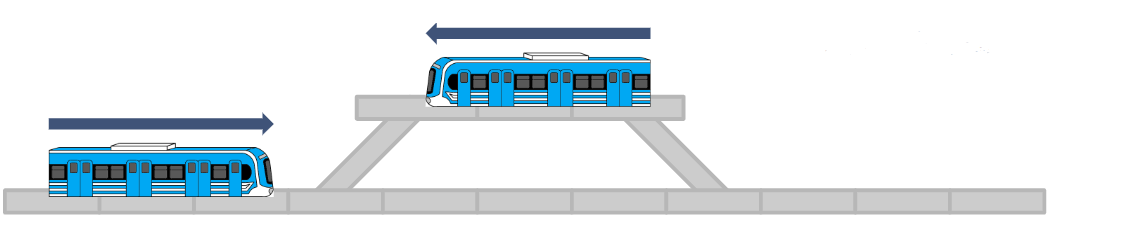
\includegraphics[width=1\textwidth]{Figuras/bypass}
        \centering\caption{Topología de derivación ferroviaria.}
        \label{fig:bypass_1}
    \end{figure}
    
Las topologías de derivación ferroviaria se utilizan principalmente para transportar materias primas entre locaciones rurales a grandes distancias de los puestos. Es deseable tanto una logística óptima, para transportar mas bienes y mas rápido, cómo un sistema seguro que garantice que los bienes lleguen a destino.
    \subsection{Simple}

En entornos urbanos donde las estaciones ferroviarias se encuentran separadas entre sí por unos pocos kilómetros es necesaria una interconectividad mayor. El sistema ferroviario debe satisfacer la demanda de una población mayor y a la vez coexistir con un trazado vehicular mucho mas denso que cruza al trazado ferroviario en varios puntos. En este contexto, una topología simple como la presentada en la Figura \ref{fig:simple_1} es una solución óptima al problema planteado.

    \begin{figure}[h]
        \centering
        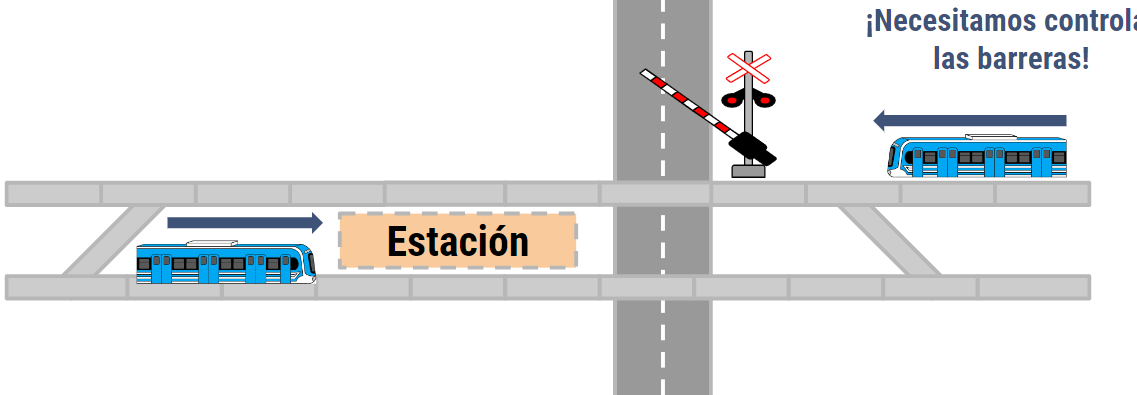
\includegraphics[width=1\textwidth]{Figuras/simple}
        \centering\caption{Topología simple.}
        \label{fig:simple_1}
    \end{figure}

El cruce entre el trazado ferroviario y el trazado vehicular se denomina paso a nivel. El sistema de enclavamientos deberá garantizar que el paso a nivel se encuentre despejado de vehículos y peatones antes de permitir la circulación de trenes sobre el mismo. Esto se logra mediante el uso de una barrera ferroviaria, un mecanismo que mantiene la barrera en alto mientras no se detecten formaciones en las proximidades del paso a nivel.

Las topologías simples suelen contar con dos vías unidireccionales en sentido ascendente y descendente. 
Las vías ascendentes son aquellas por las que las formaciones circulan en la dirección del kilometraje creciente. Mientras que las vías descendentes son aquellas por las que circulan en la dirección del kilometraje decreciente [REF]. El kilómetro cero es la estación principal de la línea ferroviaria, como por ejemplo: Plaza Constitución (Línea Roca), Once de Septiembre (Línea Sarmiento) o Retiro (Línea Mitre y Linea San Martín). Las formaciones pueden cambiar de vía ascendente a descendente, o viceversa, utilizando un cambio ferroviario.
    \subsection{Hub}

A medida que mas líneas ferroviarias coexisten en la misma red se vuelve inevitable que varias líneas compartan la misma estación utilizando diferentes plataformas en paralelo. Con una logística mas flexible, las diferentes líneas incluso pueden utilizar de forma alternada las mismas plataformas y, por lo tanto, las mismas vías principales. Además, es necesario contar con mecanismos para retirar trenes de la red para su mantenimiento y volver a inyectarlos a la red cuando la demanda aumente. Esto se logra por medio de talleres ferroviarios en las inmediaciones de las estaciones que actúan como un hub ferroviario. La topología de hub ferroviario se ilustra en la Figura \ref{fig:hub_1}.

    \begin{figure}[h]
        \centering
        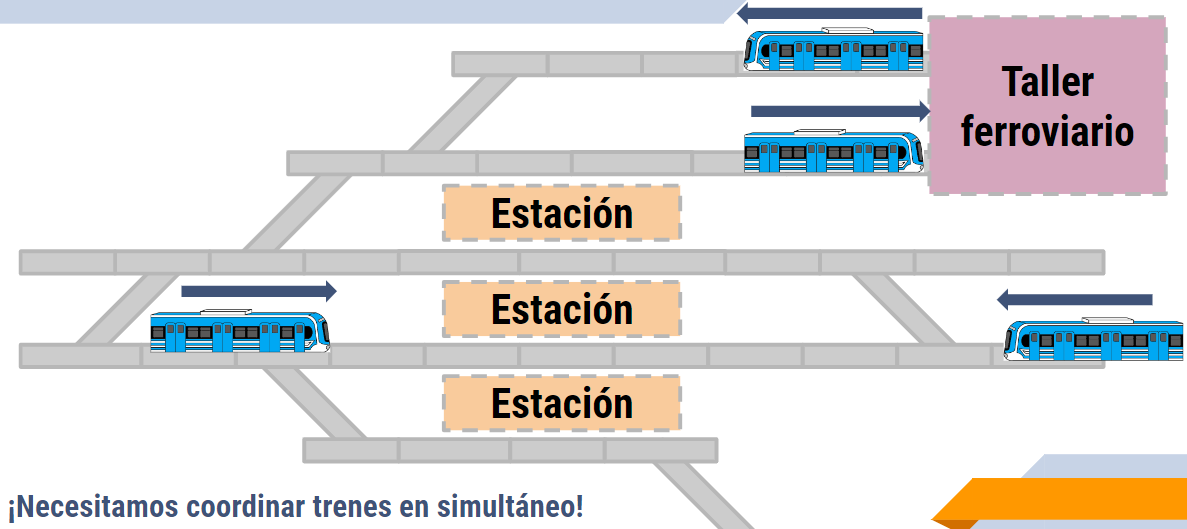
\includegraphics[width=1\textwidth]{Figuras/hub}
        \centering\caption{Topología hub.}
        \label{fig:hub_1}
    \end{figure}
    
Las tareas del sistema de enclavamientos van aumentando en complejidad a medida que se suman nuevos actores. Debe coordinar diversas formaciones de distintas líneas, accediendo a diferentes plataformas, cumpliendo diferentes horarios de arribo y partida. A su vez, debe asegurarse de que las formaciones circulen con seguridad pero sin descuidar la puntualidad. Adicionalmente, debido a que la demanda varía a lo largo del día, deberá tener flexibilidad para inyectar nuevas formaciones a la red o remover las que presenten desperfectos técnicos. Todas estas acciones deben realizarse en simultáneo y en un entorno de alto dinamismo.
    \subsection{Estación Terminal}

Las estaciones terminales presentan una gran cantidad de vías principales y plataformas en paralelo, en las cuales confluyen una o varias líneas ferroviarias. A diferencia de estaciones de tipo hub que pueden presentar finales de vía relativos, las estaciones terminales poseen finales de vía absolutos. Es decir, las formaciones que circulan por la vía descendente deberán detener su marcha completamente antes de llegar al fía de vía, para luego retomar su marcha en sentido contrario, por la vía ascendente. Esta operación puede realizarse de manera inmediata en formaciones con locomotras eléctricas en ambos extremos del tren o con locomotoras diesel luego de varias maniobras que requieren el uso de diversos cambios de vías. En la Figura \ref{fig:terminal_1} se ilustra un ejemplo de una estación terminal.

    \begin{figure}[h]
        \centering
        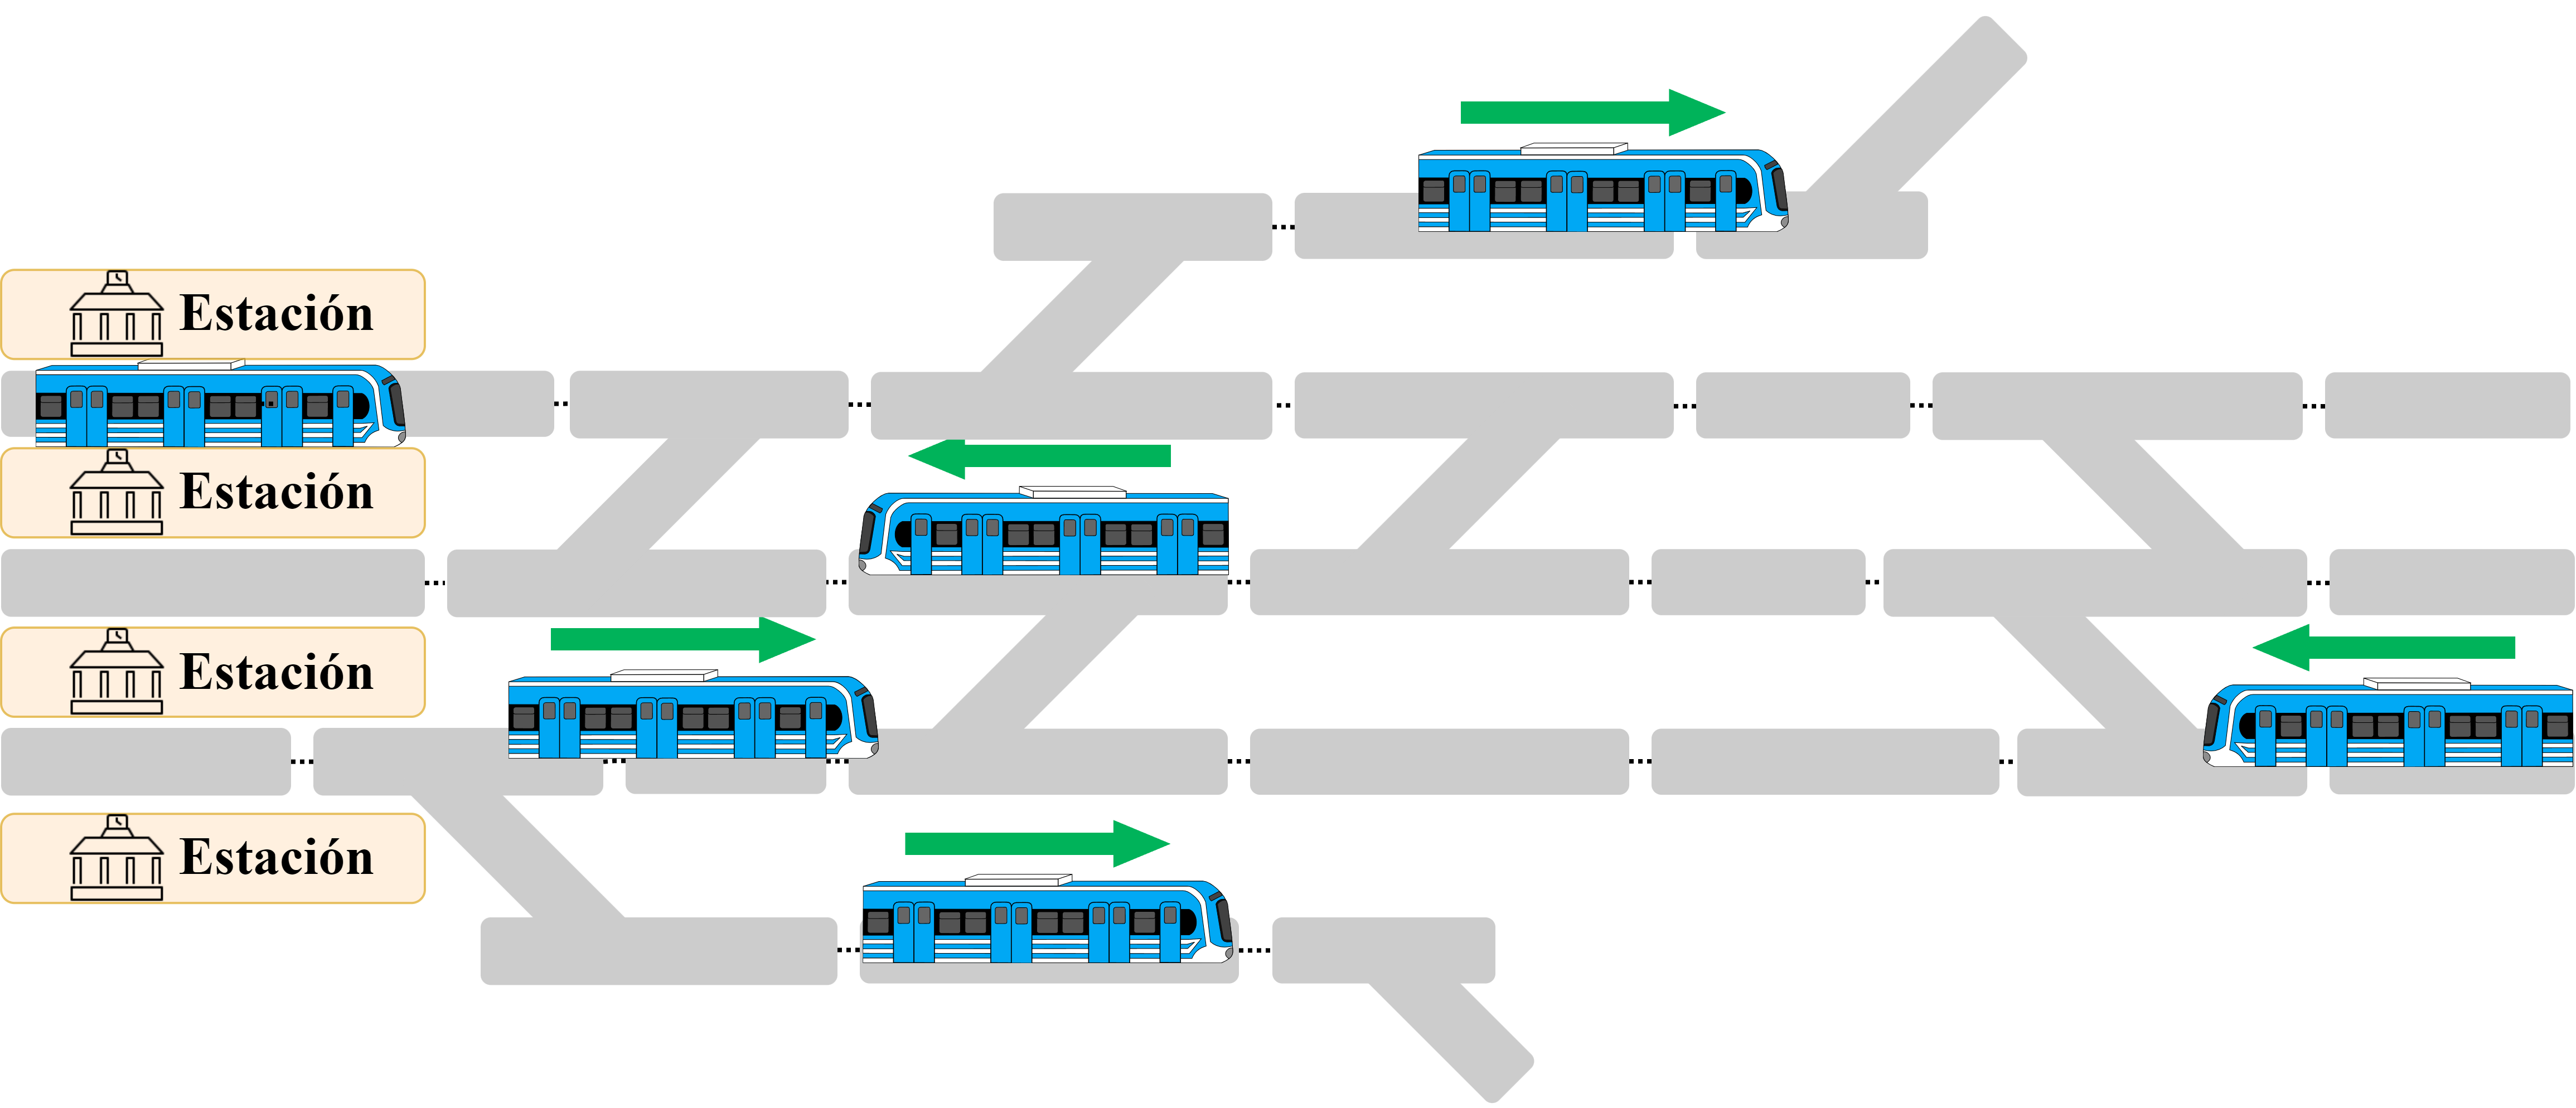
\includegraphics[width=1\textwidth]{Figuras/terminal}
        \centering\caption{Topología terminal.}
        \label{fig:terminal_1}
    \end{figure}

En las estaciones terminales suelen confluir la información en tiempo real de la terminal y las estaciones mas próximas de la línea, o incluso la información en tiempo real de la totalidad de la línea. Esta característica, además de ser la estación de mayor tamaño de la línea, les otorga una jerarquía tal que suelen concentrar parcial o totalmente el control del señalamiento de la red. Las decisiones tomadas en una estación terminal tienen un gran impacto en el sistema de transporte de toda la línea, directa o indirectamente. Estas operaciones deben considerar cientos o miles de estados en simultáneo, por lo que ejecutarlas de forma manual es muy complejo o incluso imposible. Un sistema de enclavamientos moderno, robusto, que pueda garantizar una altísima disponibilidad, mantenibilidad y seguridad es indispensable para llevar a cabo estas tareas.
\section{Estado del arte}

\lipsum[1]

\subsection{Empresas del sector ferroviario}

\lipsum[1]
\subsection{Herramientas existentes}

\lipsum[1]
\subsection{Estudios realizados}

\lipsum[1]
\subsection{Enfoque funcional vs enfoque geografico}

\lipsum[1]

\subsection{RailTopoModel}

\lipsum[1]

\input{introduccion/estado-del-arte/railTopoModel/grafos}
\input{introduccion/estado-del-arte/railTopoModel/niveles}
\subsection{RailML}
    \label{sec:railML}
    
    railML [REF] (del inglés, Railway Markup Language) es un estándar abierto de comunicación de datos entre herramientas ferroviarias desarrollado por las principales empresas de la industria ferroviaria a partir del año 2002. Las primeras dos versiones del estándar se diseñaron en base al enfoque funcional, pero en 2017 se lanzó railML 3.0, basado en RailTopoModel y, por lo tanto, adoptando un enfoque puramente geográfico.

\input{introduccion/estado-del-arte/railML/railML3}
\input{introduccion/estado-del-arte/railML/Industria}
\section{Impacto economico}

\lipsum[1]
\includegraphics{example-image}
\lipsum[1]
\newpage
\chapter{Railway Network Analyzer (RNA)}
\label{sec:RNA}

\section{Elementos ferroviarios}

El sistema ferroviario consta de diversos elementos que incluyen la infraestructura (tendido ferroviario, plataformas, cruces de vía), sensores (circuitos de vía, contadores de eje), actuadores (barreras ferroviarias, máquinas de cambios) e interfaces visuales con los conductores (semáforos ferroviarios). Todos estos elementos se interrelacionan y funcionan en conjunto dentro del sistema de señalamiento y el sistema de enclavamiento. Cada uno de estos elementos será descripto en la sucesivas secciones, en orden tal de integrar los conceptos anteriores de la forma mas clara posible.

\subsection{Vías}

Las vías férreas son el elemento ferroviario mas esencial, son la columna vertebral de la infraestructura ferroviaria. Estas constituyen el sitio por el cual se desplazan los trenes, definiendo no solo la dirección del desplazamiento, sino también restringiendo el dominio del tren. Esto lo diferencia de otros medios de transporte como el automóvil que no necesitan un camino para circular y, aún teniendo una carretera, puede moverse libremente por fuera de esta.

Las vías se encuentran separadas por una distancia fija que se mide desde sus caras internas, denominada trocha (Figura \ref{fig:vias_1}). Solamente las formaciones compatibles con ese parámetro de trocha pueden circular por el tendido ferroviario. El valor de la trocha puede variar entre las denominadas trocha angosta (600 a 1372 mm, estándar imperial británico) y trocha ancha (1520 a 3000 mm, estándar ruso, indio, ibérico, irlandés). Se estableció el valor intermedio de 1425 mm como valor de trocha internacional, usado ampliamente en Europa, Norteamérica y Oceanía.

    \begin{figure}[!h]
        \centering
        
\includegraphics[width=1\textwidth]{Figuras/trocha.png}
        \centering\caption{Vías ferroviarias y trocha.}
        \label{fig:vias_1}
    \end{figure}
    
Existen limitaciones logísticas y físicas por las cuales el tendido ferroviario no puede ser un continuo rígido. En primer lugar, las vías deben ser de un tamaño acotado, tal que puedan transportarse a la locación donde serán instaladas en tramos rectos o curvos. En segundo lugar, la dilatación y contracción de las vías debido a los cambios de temperatura añaden una restricción respecto a la distancia mínima que deben tener entre las mismas. De lo contrario, la dilatación del material puede provocar daños irreparables a la infraestructura y estos, a su vez, ser motivo de descarrilamientos, como ya ha ocurrido en los comienzos de la industria ferroviaria [REF]. 
    
Cada vía puede ser clasificada en dos grupos: vías ascendentes o vías descendentes (\ref{fig:vias_2}). Las ascendentes son aquellas por las cuales los trenes circulan únicamente en la dirección del kilometraje en sentido creciente. Las descendentes son aquellas por las cuales los trenes circulan únicamente en la dirección del kilometraje en sentido decreciente [REF]. 

    \begin{figure}[!h]
        \centering
        \includegraphics[width=1\textwidth]{example-image}
        \centering\caption{Vías ascendentes y descendentes.}
        \label{fig:vias_2}
    \end{figure}

El kilómetro 0 es la estación principal de la línea ferroviaria, como pueden ser las terminales de Plaza Constitución (para la línea Roca), Once de septiembre (para la línea Sarmiento) y Retiro (para las líneas Mitre y San Martín).  Existen vías de maniobra que pueden ser tanto ascendentes como descendentes. Estas vinculan, mediante un cambio de vías, una sección ascendente con otra descendente, en la cual los trenes deben circular a una velocidad reducida. 

Las vías se agrupan en secciones que, por cuestiones de seguridad y logística, se establece que solo pueden ser utilizadas por un tren a la vez. Estas secciones pueden ser de varios kilómetros en zonas rurales o unos pocos cientos de metros en zonas urbanas, donde la red necesita una mayor granularidad debido a la densidad del tráfico ferroviario en las grandes urbes.
\subsection{Fin de vía y transiciones}

El tendido ferroviario no puede continuar de forma indefinida, ni tampoco interrumpirse de forma abrupta. Como se puede visualizar en la Figura \ref{fig:frontera_1}, existen dos formas de definir el fin de vía: de forma relativa y de forma absoluta.

Un fin de vía relativo es todo aquel límite que define el alcance del sistema de señalamiento, pero no necesariamente es el final de la red. Es decir, el sistema podrá recibir información de cualquier sensor dentro de estos límites, o incluso de algunos sensores en la frontera exterior, pero solo podrá comandar los actuadores dentro de la zona. Esto es de vital importancia a la hora de reducir la complejidad de la red, al realizar el procesamiento de forma distribuida, sin depender de un decisión centralizada.

Un fin de vía absoluto es todo aquel límite que define el final físico del tendido ferroviario, luego del cual ya no se tiene infraestructura. Podemos encontrar estos límites en los talleres ferroviarios, en las terminales principales de cada red o en vías utilizadas para estacionar los trenes por fuera de la rama principal en uso. Estos límites deben estar adecuadamente protegidos y señalizados.

    \begin{figure}[!h]
        \centering
        \includegraphics[width=1\textwidth]{example-image}
        \centering\caption{Topología de ejemplo con finales de vía relativos y absolutos.}
        \label{fig:frontera_1}
    \end{figure}
    
En la Figura \ref{fig:frontera_1} encontramos varios casos de ambos elementos. Un ejemplo de fin de vía relativo sería la frontera entre las estaciones A y B. Las vías continúan a la derecha de A, pero no son parte del alcance del sistema que controla los elementos ferroviarios en las inmediaciones de A. En tanto que un fin de vía absoluto sería todo final literal de la red ferroviaria, tales como terminales, talleres y vías secundarias sin retorno.
\subsection{Sistemas de detección de formaciones ferroviarias}

Es de vital importancia que el sistema pueda determinar la posición de un tren dentro del tendido ferroviario. De esta manera, poder habilitar la circulación en secciones donde no exista peligro de colisión con otros formaciones o, por el contrario, detener la marcha de las formaciones anteriores para evitar accidentes. Existen diversas maneras de detectar la posición de un tren, entre ellas el uso de circuitos de vía y contadores de ejes. 

Los circuitos de vía (Figura \ref{fig:deteccion_1}) son dispositivos electrónicos que aplican una diferencia de potencial finita entre los rieles. Cuando una formación ingresa a la sección, sus ruedas metálicas cortocircuitan ambos rieles. El cortocircuito es detectado por el relé y este, a su vez, reporta el estado al resto del sistema. 

    \begin{figure}[!h]
        \centering
        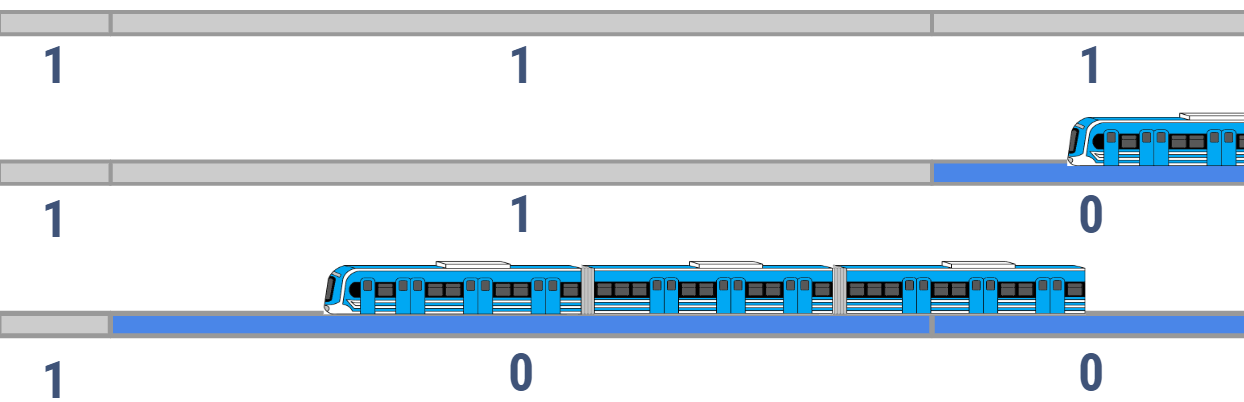
\includegraphics[width=1\textwidth]{Figuras/circuito_via}
        \centering\caption{Circuito de vía libre y ocupado.}
        \label{fig:deteccion_1}
    \end{figure}

En caso de que la alimentación se interrumpa, el cableado sufra alguna falla, vandalismo, inundación, o que efectivamente una formación ocupe la sección, el circuito de vía reportará que la sección se encuentra ocupada. De esta manera, solo es posible recibir un reporte de sección desocupada cuando la sección efectivamente se encuentre desocupada. A este principio se le denomina fail-safe [REF]. Es decir, si por alguna razón algo falla, el sistema adopta la condición más restrictiva, mitigando la posibilidad de una situación peligrosa

Los sistemas contadores de ejes (Figura \ref{fig:deteccion_2}) consisten en sensores pasivos instalados en la cara interna de unos de los rieles y un sistema externo de procesamiento de datos. Estos sistemas no dependen de la aplicación de tensiones en la vía. Además, no solo permiten detectar la presencia de una formación, sino que también pueden usarse para medir la integridad de la formación, sabiendo el largo esperado de la misma. 

    \begin{figure}[!h]
        \centering
        \includegraphics[width=1\textwidth]{example-image}
        \centering\caption{Contadores de ejes.}
        \label{fig:deteccion_2}
    \end{figure}

Al igual que los circuitos de vía, los sistemas contadores de eje siguen el principio de fail-safe, adoptando la condición mas restrictiva en caso de falla. Ambos sistemas pueden utilizarse en simultáneo, de ser requerido.
\subsection{Automatic Train Stop (ATS)}

\lipsum[1]

    \begin{figure}[!h]
        \centering
        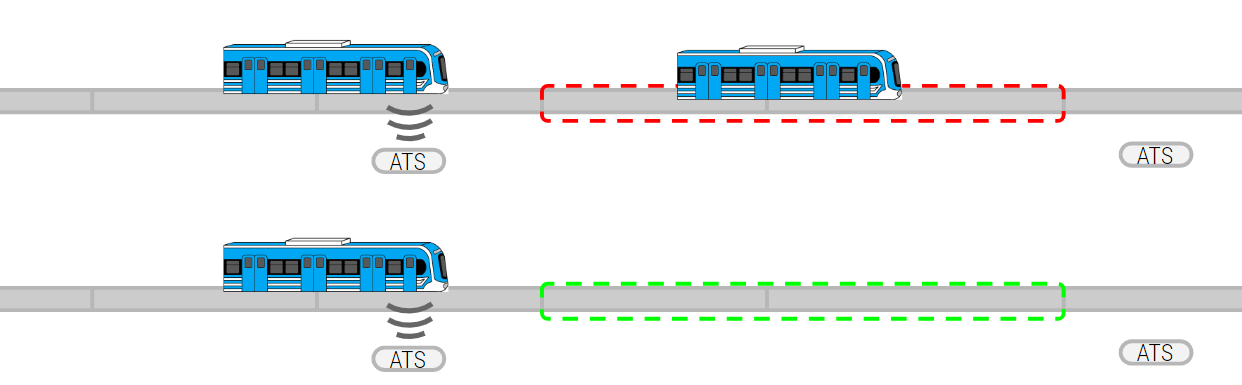
\includegraphics[width=1\textwidth]{Figuras/ATS}
        \centering\caption{ATS.}
        \label{fig:ATS_1}
    \end{figure}

\lipsum[1]
\subsection{Estaciones ferroviarias}

Las estaciones ferroviarias son las zonas donde las formaciones pueden detenerse para que los pasajeros puedan descender y nuevos pasajeros puedan abordar. En función del tamaño de las formaciones y la geografía del lugar, las plataformas desde donde ascienden y descienden los pasajeros pueden estar elevadas con respecto al suelo o a ras del mismo. El largo de las plataformas también depende de la cantidad de coches de las formaciones.

Como puede verse en la Figura \ref{fig:estacion_1}, las estaciones ferroviarias incluyen no solo a las plataformas, sino que también pueden centralizar el control de varias operaciones logísticas como la asignación de rutas. No obstante, en este trabajo nos referiremos a las estaciones como plataformas indistintamente.

    \begin{figure}[!h]
        \centering
        \includegraphics[width=1\textwidth]{example-image}
        \centering\caption{XXXXX.}
        \label{fig:estacion_1}
    \end{figure}

Las estaciones de mayor complejidad o de mayor convergencia de ramales suelen concentrar el control de la estación donde se encuentran y varias estaciones vecinas. Las estaciones terminales, a menudo, pueden incluso tener control total de varios ramales completos.
\subsection{Cruces ferroviarios}

Los cruces ferroviarios son la intersección entre la vía ferroviaria y una ruta vehicular o peatonal. Estos cruces pueden ser bajo nivel (túnel por debajo de la vía), sobre nivel (puente vehicular por sobre la vía) o a nivel. Un paso a nivel es una zona muy crítica del sistema ferroviario, ya que, a diferencia de un paso sobre nivel o bajo nivel, conviven simultáneamente la formación y el transito vehicular y peatonal. En la Figura \ref{fig:cruce_1} se ilustra la intersección entre el tendido ferroviario, un cruce vehicular y un cruce peatonal.

    \begin{figure}[!h]
        \centering
        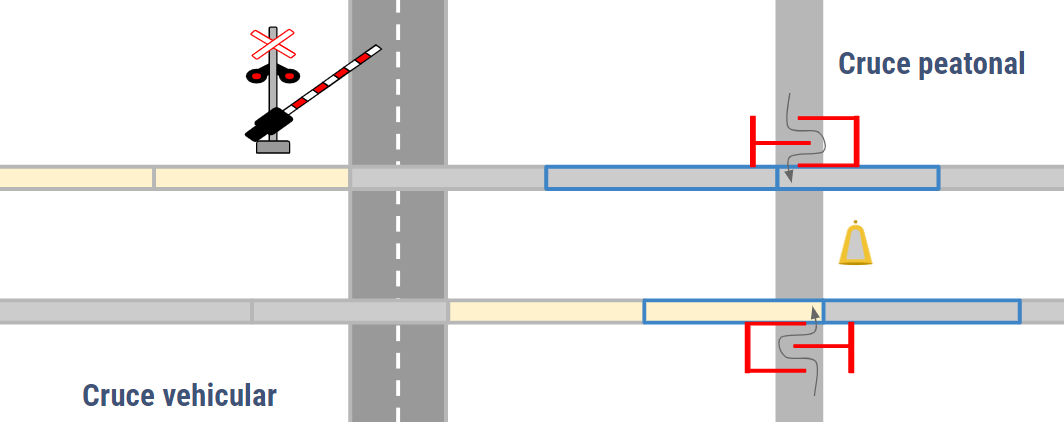
\includegraphics[width=1\textwidth]{Figuras/cruce}
        \centering\caption{XXXXX.}
        \label{fig:cruce_1}
    \end{figure}
    
Los pasos a nivel peatonales incluyen un pequeño laberinto zigzagueante para forzar al peatón a aminorar su marcha y ver a ambos lados antes de cruzar las vías. A menudo suelen estar acompañados de indicaciones lumínicas y sonoras que se accionan tan pronto el tren se encuentre dentro de un rango de varios metros cercano al paso a nivel.

Los pasos a nivel vehiculares añaden barreras ferroviarias para detener el tráfico vehicular cuando un tren se encuentra dentro de un rango de seguridad definido.  El sistema de control de la barrera mantiene el brazo de esta en alto para permitir la circulación vehicular. Si un tren es detectado cerca del paso a nivel, se desenergiza la barrera y comienza a descender el brazo por efecto de la gravedad. Solo cuando la barrera baja, el tren tiene permitido avanzar sobre el cruce, siendo el paso a nivel un sector de altísimo riesgo. Al desocuparse las secciones próximas al paso a nivel, la barrera vuelve a energizarse y se sitúa en estado alto nuevamente, a la espera de otro tren para reiniciar el proceso. 

Se debe destacar que el mismo proceso de descenso de la barrera ocurrirá si esta se desenergiza por una falla electricomecánica y/o pérdida de alimentación. Es decir, el sistema asumirá el estado más seguro ante cualquiera de los mencionados fallos, siguiendo el principio de falla segura.
\subsection{Máquina de cambios}

    Una máquina de cambios (Figura \ref{fig:cambios_1}) es un mecanismo utilizado para permitir el paso de las formaciones de una vía a una ramificación del recorrido principal. Esto se realiza mediante el movimiento de la aguja del cambio (riel móvil) hacia su respectiva contraaguja (riel fijo) hasta obtener un adecuado acoplamiento que permita la circulación de la formación.

    \begin{figure}[!h]
        \centering
        \includegraphics[width=1\textwidth]{example-image}
        \centering\caption{XXXXX.}
        \label{fig:cambios_1}
    \end{figure}

    En la Figura \ref{fig:cambios_2} se muestra el cambio de vía de la estación Matheu de la Línea Mitre. Se observa que según sea la posición de la máquina de cambios, el tren puede continuar en la misma vía o hacer el cambio a la otra vía.

    \begin{figure}[!h]
        \centering
        \includegraphics[width=1\textwidth]{example-image}
        \centering\caption{XXXXX.}
        \label{fig:cambios_2}
    \end{figure}

    En la Figura \ref{fig:cambios_3} se muestran las posiciones que puede adoptar el cambio. En la posición normal, los trenes pueden circular de forma directa, en paralelo, por la vía principal en sentidos opuestos. En la posición reversa, en cambio, se permite el intercambio de trenes de una rama principal a otra en sentido opuesto o a una ramificación secundaria de la red.

    \begin{figure}[!h]
        \centering
        \includegraphics[width=1\textwidth]{example-image}
        \centering\caption{XXXXX.}
        \label{fig:cambios_3}
    \end{figure}

    Hablar de comando, correspondencia y accion. Figura \ref{fig:cambios_4}

    \lipsum[1]
    
    \begin{figure}[!h]
        \centering
        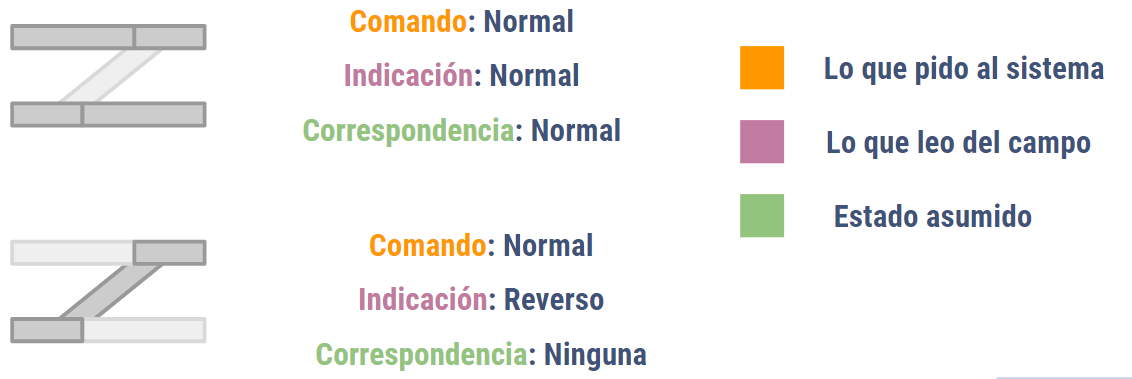
\includegraphics[width=1\textwidth]{Figuras/cambios}
        \centering\caption{XXXXX.}
        \label{fig:cambios_4}
    \end{figure}

EXPLICAR MAS DE CAMBIOS
\subsection{Señales ferroviarias}

El sistema de señalamiento utiliza los semáforos ferroviarios (en adelante denominados señales) para indicarle al conductor del tren si tiene autoridad de tránsito en al próximo tramo de vías y a qué velocidad se le permite circular; esto, por medio del color del semáforo, denominado aspecto. A diferencia de los semáforos vehiculares, en los que cada color es alternado por otro de la secuencia rojo-amarillo-verde en función del tiempo, los semáforos ferroviarios cambian su aspecto en función de los eventos de los tramos siguientes. En la Figura \ref{fig:signal_1} se presenta un esquema de señales de tres aspectos, que es el tipo de semáforo que se utiliza en la gran mayoría de las líneas ferroviarias.

    \begin{figure}[!h]
        \centering
        \includegraphics[width=1\textwidth]{example-image}
        \centering\caption{XXXXX.}
        \label{fig:signal_1}
    \end{figure}

Otra diferencia fundamental es que no todos los semáforos ferroviarios poseen tres aspectos. Los semáforos de maniobras constan de solo dos, amarillo (precaución) y rojo (prohibido avanzar), y algunas líneas, como la Línea Roca, utilizan semáforos de cuatro aspectos. En la Figura \ref{fig:signal_2} se visualizan los semáforos de dos aspectos. Se utilizan en cambios de vías donde, por su peligrosidad, solo se podrían permitir aspectos rojos y amarillos.

    \begin{figure}[!h]
        \centering
        \includegraphics[width=1\textwidth]{example-image}
        \centering\caption{XXXXX.}
        \label{fig:signal_2}
    \end{figure}

Los semáforos de cuatro aspectos son utilizados en la Línea Roca y poseen un doble amarillo antes del amarillo simple, para permitir así tramos de vías más cortos de forma segura. Como no son objeto de estudio del presente trabajo, no serán explicados aquí. (EDITAR)

    \begin{figure}[!h]
        \centering
        \includegraphics[width=1\textwidth]{example-image}
        \centering\caption{XXXXX.}
        \label{fig:signal_3}
    \end{figure}

EXPLICAR MAS LOS SEMAFOROS.

\section{Biblioteca RailML}

    El primer paso en el desarrollo del RNA es contar con una librería que permita generar un objeto equivalente uno a uno con el estándar railML y luego exportar un nuevo archivo railML. Como ya se mencionó en la Sección \ref{sec:railML}, el estándar railML define cinco clases de objetos principales: Common, Infraestructure, Interlocking, RollingStock y Timetable. 

    La clase Common incluye 109 subclases, todas ellas utilizadas para definir características generales e invariantes para la red. Por ejemplo, podemos encontrar la clase Concessionaire que define quien tiene la concesión de la red, la clase tBrakeType que define el tipo de frenos aceptados en esa red, la clase tVoltage que define la tensión de la red o la clase PublicHolidayPeriodRule que define el período de vacaciones de los operarios de la red, entre otros factores. Esta clase es obligatoria para todos los archivos en formato railML, por lo tanto es necesaria para el funcionamiento del RNA, aunque no se extraigan datos importantes de la misma.

    La clase Infraestructure incluye  231 subclases, todas ellas enfocadas en definir las características estáticas de cada elemento ferroviario, como su posición, dimensiones y demás parámetros invariantes en el tiempo.  Entre ellas podemos encontrar la clase Borders (ver Sección XX), BufferStops (ver Sección XX), LevelCrossingsIS (ver Sección XX), Platforms (ver Sección XX), SignalsIS (ver Sección XX), SwitchesIS (ver Sección XX) y Tracks (ver Sección XX), entre otras. Adicionalmente incluye dos clases fundamentales para el análisis de redes de grafos: netElement y netRelation, ambas discutidas en la Sección XX. En el caso de hacer análisis a nivel meso y macroscópico se tienen, además, las clases Line, OperationalPoint y Network, no cubiertas en este análisis.

    La clase Interlocking incluye 156 subclases, todas ellas enfocadas en definir las características dinámicas de los elementos ferroviarios que las posean. Entre ellas podemos encontrar LevelCrossingsIL (ver Sección XX), SignalsIL (ver Sección XX), SwitchesIL (ver Sección XX), entre otras. Adicionalmente, se encuentras las subclases relacionadas a la tabla de enclavamientos y las rutas, como Routes, CombinedRoutes, ConflictingRoutes, RoutesRelations y muchas otras referidas explícitamente a rutas (ver Sección XX). 
    
    El RNA solamente necesita de las clases Common, Infraestructure e Interlocking para funcionar, por lo que no fue necesario implementar las clases RollingStock ni Timetable. En total se han implementado 524 clases, considerando 28 clases nativas de RailTopoModel necesarias para que railML pueda interpretar los tipos de datos definidos. Todas las clases y subclases mencionadas son opcionales en el estándar, salvo que se indique lo contrario, es decir, no son obligatorias para que el archivo railML se considere válido.

    En las siguientes secciones se detallaran las subclases mas importantes implementadas, tal que se pueda comprender que atributos son procesados para poder generar el señalamiento. Se comenzará con las clases relativas a la topología de la red, eje central análisis del RNA y se proseguirá con las clases asociadas a elementos ferroviarios materiales. Simultáneamente, se profundizará en los conceptos mas destacados de cada elemento ferroviario correspondiente a esa clase, destacando cual es el señalamiento asociado al mismo para protegerlo en base a los principios ferroviarios expuestos.

    % COMMON
    \subsection{Campo de metadatos}
    \label{sec:metadata}

    Aunque no es una clase de railML, el campo metadata es fundamental para que el archivo en formato railML sea válido. Se presenta el Código \ref{lst:metadata} para ilustrar los elementos presentes en la sección de metadatos.
    
    \begin{lstlisting}[language = XML, caption = Campo de metadatos, label = {lst:metadata}]
<metadata>
    <dc:title>Example_9.railml</dc:title>
    <dc:date>2023-10-04T10:51:21Z</dc:date>
    <dc:creator>Trenes_Argentinos</dc:creator>
    <dc:source>RaIL-AiD</dc:source>
    <dc:identifier>1</dc:identifier>
    <dc:subject>railML.org</dc:subject>
    <dc:format>0.9.5</dc:format>
    <dc:description>Ejemplo_real</dc:description>
    <dc:publisher>RaIL-AiD framework</dc:publisher>
</metadata>
    \end{lstlisting}

    Ninguno de estos campos es esencial para el funcionamiento del RNA, por lo que son copiados sin cambios al nuevo archivo generado. No obstante, la ausencia de alguno de estos campos o que el campo sea nulo provoca que tanto el RNA como cualquier herramienta compatible con railML considere al archivo como incompleto o corrupto.
    \subsection{Clase common}
    \label{sec:common}

    La clase Common define todos los parámetros que son invariantes a toda la red. Esta clase puede ser definida solo una vez o no definirse. Sus subclases son:

    \begin{itemize}
        \item ElectrificationSystems: define la tensión y frecuencia de la red eléctrica.
        \item OrganizationalUnits: define quien administra la infraestructura, quien fabrica y opera el material rodante, quien es el cliente final, quien es el contratista y quien posee la concesión del servicio. 
        \item SpeedProfiles: define el perfil de aceleración, velocidades y frenado.
        \item Positioning: define los sistemas de posicionamiento geométrico, linear y referido a la pantalla del editor.
    \end{itemize}

    Cada uno de sus campos internos es único, pero también son opcionales. A modo de ejemplo se muestra el Código \ref{lst:common}, donde se ilustra como no todas las subclases han sido definidos.
    
    \begin{lstlisting}[language = XML, caption = Clase Common , label = {lst:common}]
<common id="co_01">
    <organizationalUnits>
        <infrastructureManager id="im_01"/>
    </organizationalUnits>
    <positioning>
        <geometricPositioningSystems>
            <geometricPositioningSystem id="gps01">
                <isValid from="2023-07-26" to="2024-07-26"/>
                <name name="Example_9.railml" language="en"/>
            </geometricPositioningSystem>
        </geometricPositioningSystems>
        <linearPositioningSystems>
            <linearPositioningSystem linearReferencingMethod="absolute" 
            startMeasure="0" endMeasure="0" units="Km" id="loc-1">
                <isValid from="2023-07-26" to="2024-07-26"/>
                <name name="Loc-1" language="en"/>
            </linearPositioningSystem>
        </linearPositioningSystems>
    </positioning>
</common>
    \end{lstlisting}

    Solamente los subclases OrganizationalUnits y Positioning fueron definidas, pero tanto el RNA como el estándar railML en el que el RNA se basa consideran válido a este fragmento de código. Los vectores son definidos en plural, como en el caso de geometricPositioningSystems cuyo primer, y único elemento en este caso, es geometricPositioningSystem con id="gps01". Es habitual ver estos vectores a lo largo de todo el archivo y será esencial poder determinar su dimensión.

    
    % GRAFOS
    \subsection{Infraestructura y redes de grafos}
    \label{sec:grafos}

    La clase Infraestructure define todos los elementos ferroviarios con características físicas, materiales y estáticas. Las clases que contiene son:

    \begin{itemize}
        \item Topology: define la topología de la red mediante las clases netElements y netRelationships. Incluye también la clase Network para cumplir con el estándar de RailTopoModel.
        \item Geometry: define el sistema geométrico utilizado entre las clases HorizontalCurve (en base al largo y el ángulo formado), GradientCurves (en base al largo y al gradiente ded la curva) y GeometryPoints (en base a una combinación de las dos clases anteriores).
        \item FunctionalInfrastructure: define todos los elementos ferroviarios que el RNA analizará.
        \item PhysicalFacilities: actualmente el estándar lo define vacío, sin ninguna clase interna salvo la clase Any que puede ser utilizada como comodín.
        \item InfrastructureVisualizations: define las coordenadas y estructura del elemento ferroviario en base a sus clases tRef (para indicar a que elemento afecta), SpotProjection (coordenada del elemento), LinearProjection (en caso de ser un elemento lineal) y AreaProjection (en caso de ser un elemento bidimensional).
        \item InfrastructureStates: define la validez de los datos referidos a cada elemento ferroviario.
    \end{itemize}

    Para realizar el análisis de la red, el RNA debe centrarse en tres de estas clases: Topology (para conocer cómo es la red), FunctionalInfrastructure (para conocer qué elementos tiene la red) y InfrastructureVisualizations (para conocer dónde está cada elemento ferroviario).

    Empezando por la clase Topology, existen dos clases esenciales para este análisis: la clase netElements y la clase netRelationships. Ambas son clases vectores, constituidas por clases mas pequeñas: netElement y netRelationship. Un ejemplo de la clase netElement se puede ver en el Código \ref{lst:netElement}.
    
    \begin{lstlisting}[language = XML, caption = Clase netElement , label = {lst:netElement}]
<netElement id="ne3">
    <associatedPositioningSystem id="ne3_aps01">
        <intrinsicCoordinate intrinsicCoord="0" id="ne3_aps01_ic01">
            <geometricCoordinate x="9384.050" y="0.000" positioningSystemRef="gps01"/>
        </intrinsicCoordinate>
        <intrinsicCoordinate intrinsicCoord="1" id="ne3_aps01_ic02">
            <geometricCoordinate x="7584.770" y="0.000" positioningSystemRef="gps01"/>
        </intrinsicCoordinate>
    </associatedPositioningSystem>
    <relation ref="nr_ne3ne46_swi77"/>
    <relation ref="nr_ne3ne53_swi77"/>
</netElement>
    \end{lstlisting}
    
    Los elementos mas importantes a destacar en el Código \ref{lst:netElement} son el id, el geometricCoordinate y el relation. De estos parametros podemos saber que el netElement es referido como "ne3", comienza en la coordenada (9384.050 ; 0.000) y termina en la coordenada (7584.770 ; 0.000). Además, ne3 se encuentra relacionado a los netElement ne46 y ne53 mediante un elemento referido como swi77, que mas adelante veremos que se trata de una máquina de cambios.

    Los netElement son los nodos de la red de grafos, pero estos no son puntuales, sino que son bidimensionales. Debido a que la componente x de la coordenada de inicio de ne3 es mayor que la componente x de la coordenada final de ne3, podemos deducir que ne3 se encuentra definido de derecha a izquierda. Conocer la orientación del netElement será importante a la hora de definir la circulación, información necesaria para generar las rutas.

    La clase netRelation son las aristas de la red de grafos que relacionan dos netElements entre sí. En el Código \ref{lst:netRelation} se muestra un ejemplo de los netRelation que vinculan a los netElement ne3, ne46 y ne53.    
    
    \begin{lstlisting}[language = XML, caption = Clase netRelation , label = {lst:netRelation}]
<netRelation navigability="Both" positionOnA="1" positionOnB="1" id="nr_ne3ne46_swi77">
    <elementA ref="ne3"/>
    <elementB ref="ne46"/>
</netRelation>
<netRelation navigability="Both" positionOnA="1" positionOnB="1" id="nr_ne3ne53_swi77">
    <elementA ref="ne3"/>
    <elementB ref="ne53"/>
</netRelation>
<netRelation navigability="None" positionOnA="1" positionOnB="1" id="nr_ne46ne53_swi77">
    <elementA ref="ne46"/>
    <elementB ref="ne53"/>
</netRelation>
    \end{lstlisting}
    
    La primer netRelation es entre el netElement ne3 y el ne46, la segunda netRelation es entre el netElement ne3 y el ne53. Esto es consistente con los parámetros de relation que tenía el netElement ne3 en el Código \ref{lst:netElement}. Sin embargo, en el tercer netRelation vemos que existe una relación entre los netElement ne46 y ne53 pero, en este caso, el parámetro navigability es "None", a diferencia de los primeros dos que era "both". La navegabilidad es el parámetro que hace que una red de grafos tenga sentido como red ferroviaria: que exista una conexión no implica que sea físicamente utilizable por un tren, tal como se explicó en la Sección \ref{sec:RTM}.
    
    % Explicar analisis de red de grafos
    La secuencia de análisis de la red de grafos se describe en el Algoritmo \ref{alg:graph_network}. Tanto el Algoritmo \ref{alg:graph_network} como todos los algoritmos pertenecientes al RNA y el ACG fueron diseñados e implementados durante el transcurso del presente doctorado. Estos algoritmos no son parte de ningún estándar ni trabajo previo ajeno a este desarrollo, por lo que son una pieza fundamental y original de esta tesis.    
    
    El primer paso es procesar la clase netElements para obtener un diccionario de todos los nodos de la red. Ordenar este diccionario es importante para agilizar la búsqueda de rutas más adelante. El criterio de ordenamiento fue por coordenadas, de menor a mayor, priorizando la coordenada x por sobre la y, pero cualquier otro criterio sería válido. Con el diccionario de nodos y analizando la clase netRelations es posible construir un diccionario de netPaths. Este diccionario utiliza cada nodo del grafo como índice y contiene un diccionario con todos los nodos que son vecinos anteriores y posteriores (considerando el criterio de ordenamiento, algunos nodos estarán antes o después).
    
        \begin{algorithm}\captionsetup{labelfont={sc,bf}, labelsep=newline}
            \caption{Análisis de la red de grafos}
            \label{alg:graph_network}
            \begin{algorithmic}
                \STATE \{nodes\} $\gets$ get\_nodes(netElements)
                \STATE  order\_nodes(\{nodes\})
                \STATE \{netPaths\} $\gets$ get\_relations(\{nodes\},netRelations)
                \STATE \{neighbours\} $\gets$ get\_neighbours(\{netPaths\})
                \STATE \{switches\} $\gets$ get\_switches(\{nodes\},\{neighbours\})
                \STATE \{limits\} $\gets$ get\_limits(\{nodes\})
                \STATE analyze\_connectedness(\{netPaths\})
            \end{algorithmic}
        \end{algorithm}

    La cantidad de vecinos de cada nodo es fundamental para poder clasificarlos. Los nodos que poseen un solo vecino serán nodos que se encuentren en el límite de la red (límite relativo o absoluto). Aquellos con dos vecinos, uno anterior y otro posterior, son nodos normales. En cambio, si tienen dos vecinos y ambos son anteriores o ambos son posteriores entonces son nodos que con toda seguridad tienen una máquina de cambios. Por ejemplo, el nodo ne3 del Código \ref{lst:netRelation} posee una máquina de cambios ya que los nodos ne46 y ne53 son anteriores a ne3.

    A continuación, es necesario determinar la conexidad de la red. Una red de grafos puede ser como alguna de las ilustradas en la Figura \ref{fig:conexidad}. Las redes de grafos que tengan nodos aislados o una cantidad de vecinos tales que ese nodo no represente a ninguna máquina de cambios existente no podrán ser consideradas una red ferroviaria. La red no tiene que ser totalmente conexa, se admiten redes ferroviarias disjuntas, siempre que cada red funcione de manera independiente, con una cantidad mínima de nodos en cada una.   

    \begin{figure}[!h]
        \centering
        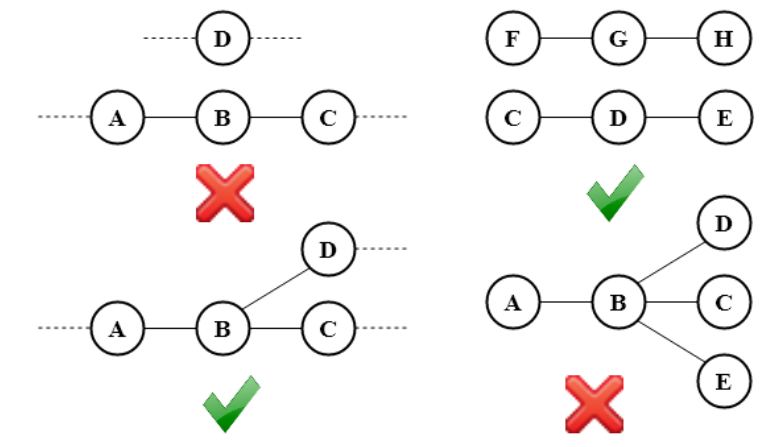
\includegraphics[width=1\textwidth]{Figuras/conexo.PNG}
        \centering\caption{Distintos tipos de redes de grafos.}
        \label{fig:conexidad}
    \end{figure}

    Para determinar si la red es conexa, se siguen los pasos del Algoritmo \ref{alg:connectedness}. Añadiendo nodos a una lista de zonas siempre que el nodo tenga un vecino en esa lista. Si un nodo posee un vecino en ambas listas, las listas se combinan, creando una nueva zona. Si la cantidad de zonas es uno entonces la red es fuertemente conexa. Una red ferroviaria disconexa puede resolverse mas rápido que una fuertemente conexa ya que no haría falta iterar entre todos los elementos para analizarlos sino solo los pertenecientes a dicho subgrafo.
        
    \begin{algorithm}\captionsetup{labelfont={sc,bf}, labelsep=newline}
        \label{alg:connectedness}
        \caption{Algoritmo de conexidad}
        \begin{algorithmic}
            \STATE \{zones\} $\gets \{ \}$
            \STATE ADD first node in \{zones\}
            \FOR {node in \{nodes\}}
                \FOR {zone in \{zones\}}
                    \IF {node not in zones[zone]}
                        \IF {neighbours(node) in zones[zone]}
                            \STATE zones[zone] ADD node
                        \ELSE
                            \STATE Define new\_zone
                            \STATE zones[new\_zone] ADD node
                        \ENDIF
                    \ENDIF
                \ENDFOR
            \ENDFOR 
            \OUTPUT \{zones\}   
        \end{algorithmic}
    \end{algorithm}
        
    En las siguientes subsecciones se analizaran en conjunto los elementos ferroviario descriptos en las clases FunctionalInfrastructure y InfrastructureVisualizations.
    
     % ELEMENTOS
    \subsection{Vías}
	\label{sec:tracks}
	
    Las vías férreas son el elemento ferroviario mas esencial, son la columna vertebral de la infraestructura ferroviaria. Estas constituyen el sitio por el cual se desplazan los trenes, definiendo no solo la dirección del desplazamiento, sino también restringiendo el dominio del tren. Esto lo diferencia de otros medios de transporte como el automóvil que, aún teniendo una carretera, puede moverse por fuera de esta.

    Las vías se encuentran separadas por una distancia fija que se mide desde sus caras internas, denominada trocha (Figura \ref{fig:vias_1}). Solamente las formaciones compatibles con ese parámetro de trocha pueden circular por el tendido ferroviario. El valor de la trocha puede variar entre las denominadas trocha angosta (600 a 1372 mm, estándar imperial británico) y trocha ancha (1520 a 2140 mm, estándar ruso, indio, ibérico, irlandés). Se estableció el valor intermedio de 1435 mm como valor de trocha internacional, usado ampliamente en Europa, Norteamérica y Oceanía.

    \begin{figure}[H]
        \centering
        
\includegraphics[width=1\textwidth]{Figuras/trocha.png}
        \centering\caption{Vías ferroviarias y trocha.}
        \label{fig:vias_1}
    \end{figure}
    
    Existen limitaciones logísticas y físicas por las cuales el tendido ferroviario no puede ser un continuo rígido. En primer lugar, las vías deben ser de un tamaño acotado, tal que puedan transportarse a la locación donde serán instaladas en tramos rectos o curvos. En segundo lugar, la dilatación y contracción de las vías debido a los cambios de temperatura añaden una restricción respecto a la distancia mínima que deben tener entre las mismas. De lo contrario, la dilatación del material puede provocar daños irreparables a la infraestructura y estos, a su vez, ser motivo de descarrilamientos, como ya ha ocurrido en los comienzos de la industria ferroviaria \cite{ACCIDENTE}. 
    
    Cada vía puede ser clasificada en dos grupos: vías ascendentes o vías descendentes (ver Figura \ref{fig:vias_2}). Las ascendentes son aquellas por las cuales los trenes circulan únicamente en la dirección del kilometraje en sentido creciente. Las descendentes son aquellas por las cuales los trenes circulan únicamente en la dirección del kilometraje en sentido decreciente \cite{RITO}. 

    \begin{figure}[H]
        \centering
        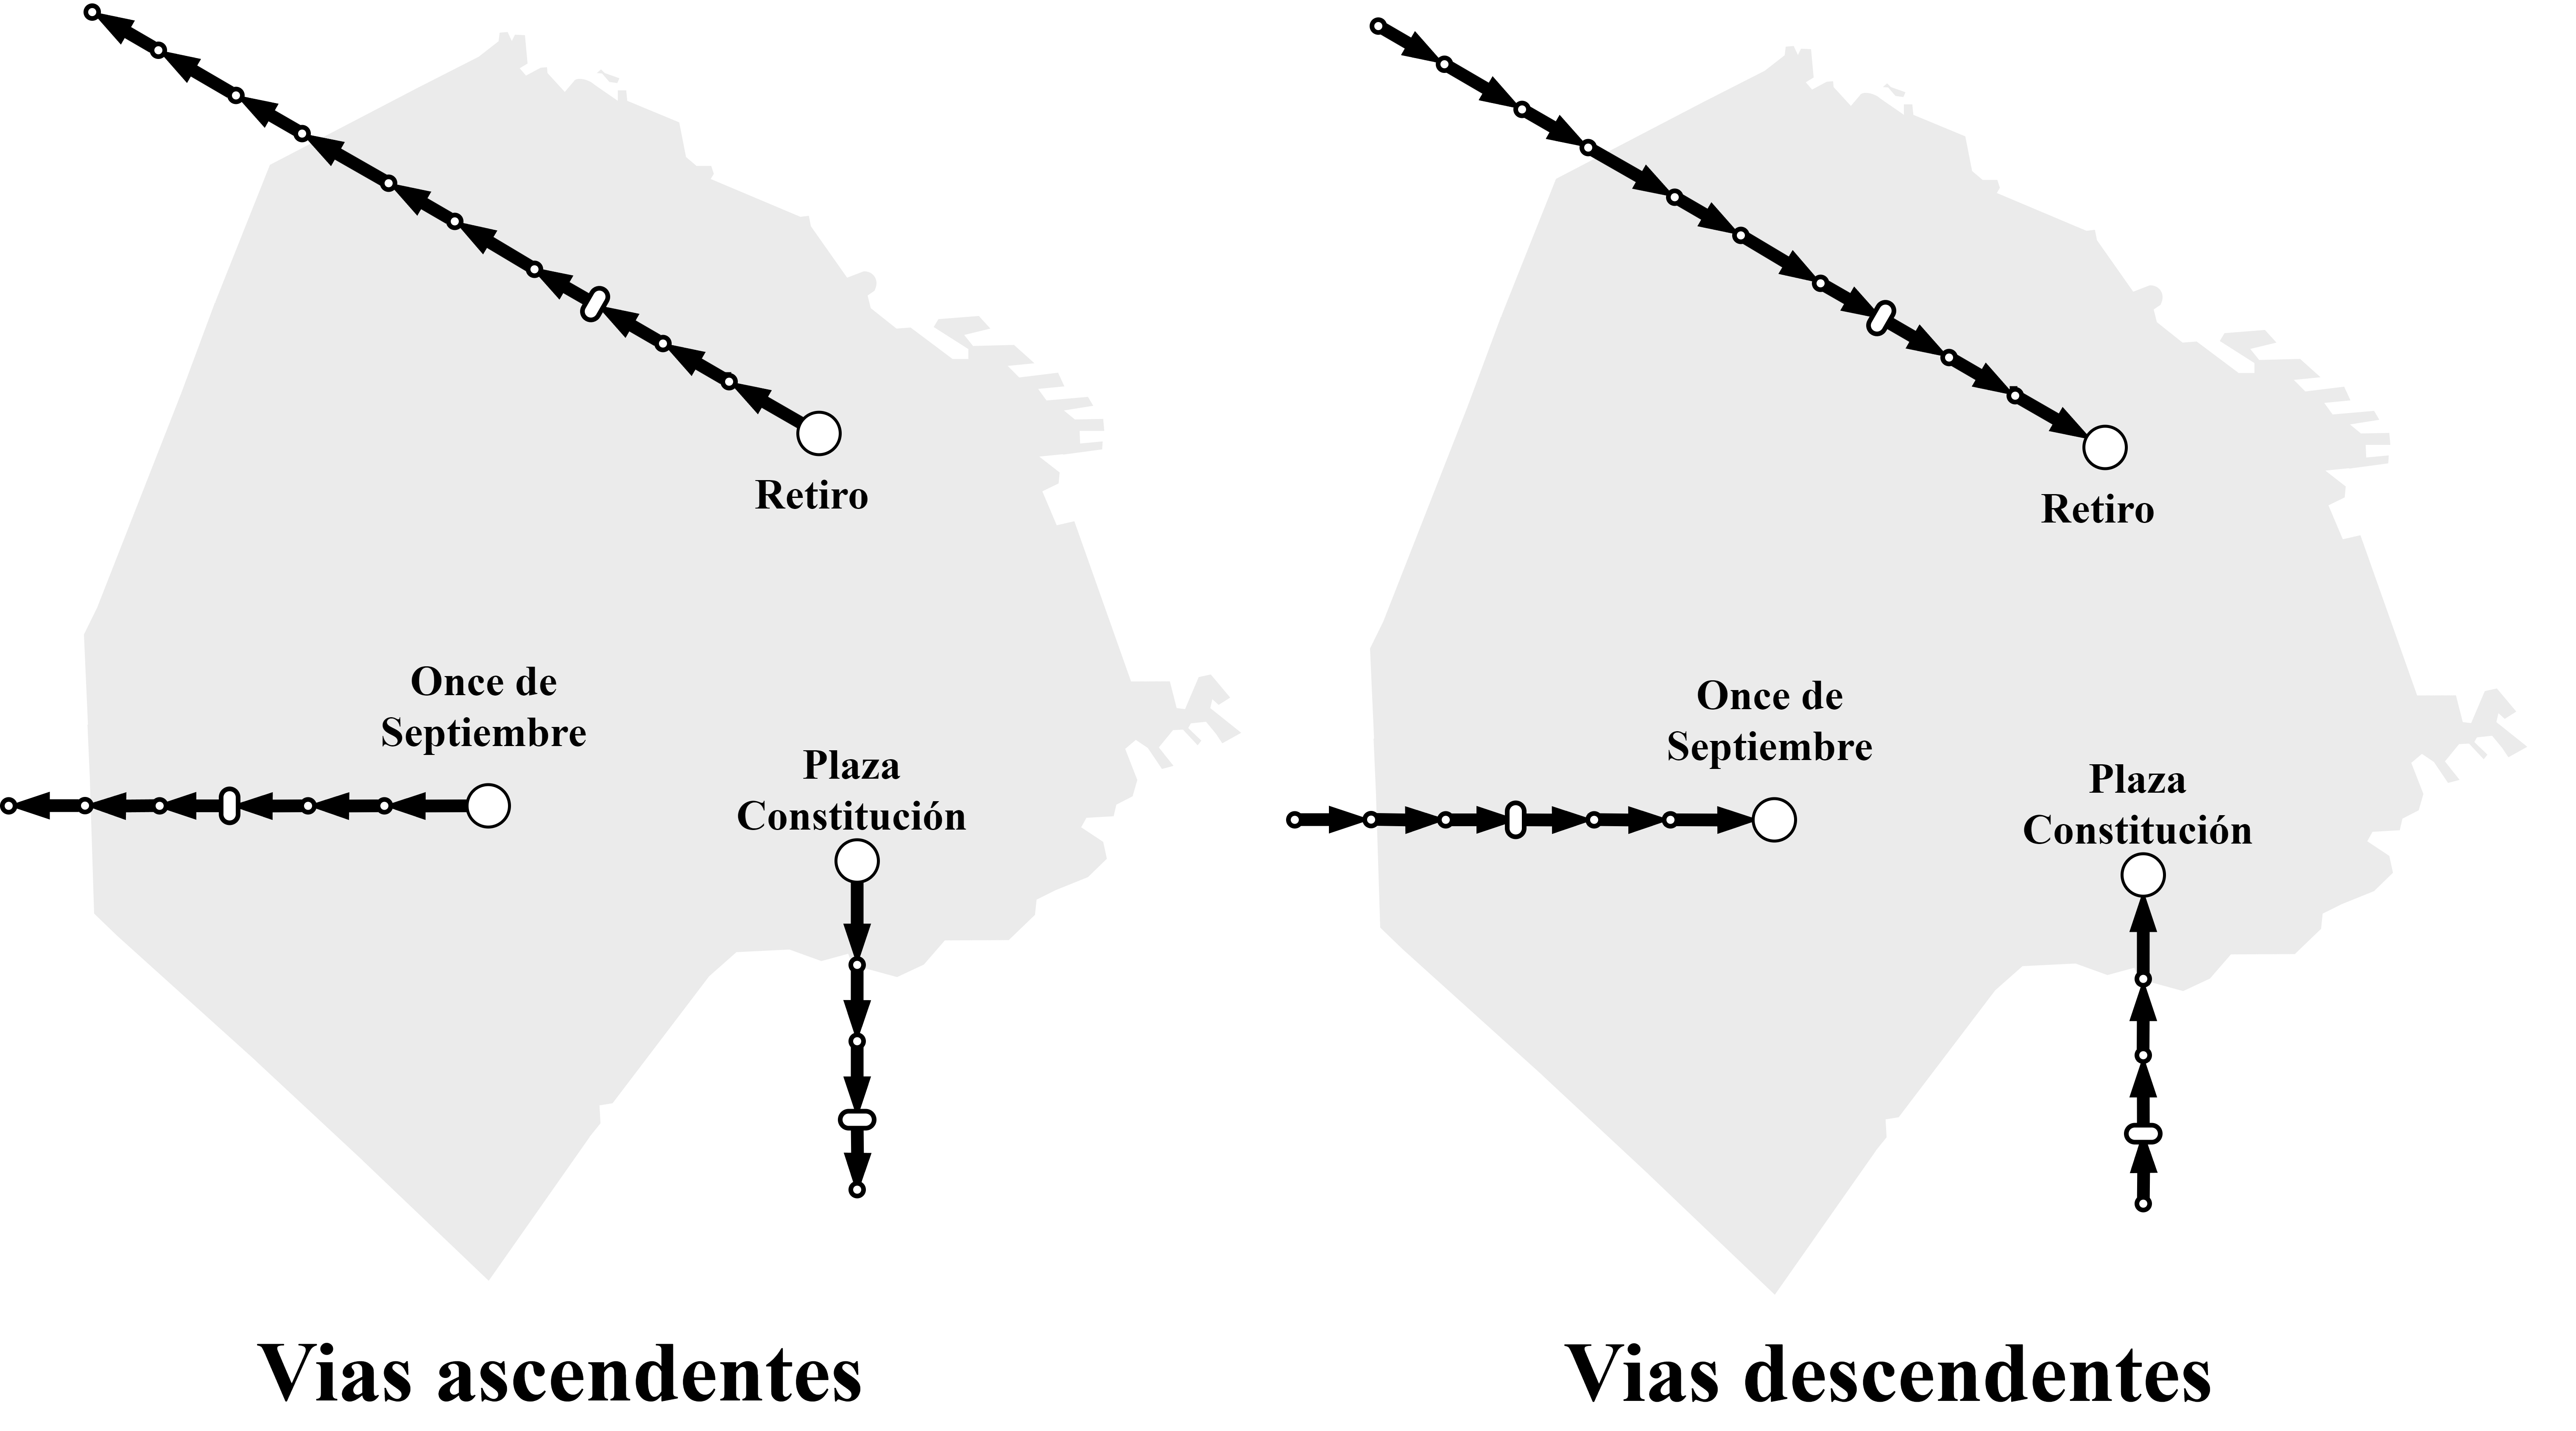
\includegraphics[width=1\textwidth]{Figuras/ascDesc.png}
        \centering\caption{Vías ascendentes y descendentes.}
        \label{fig:vias_2}
    \end{figure}

    El kilómetro cero es la estación principal de la línea ferroviaria, como pueden ser las terminales de Plaza Constitución (para la línea Roca), Once de septiembre (para la línea Sarmiento) y Retiro (para las líneas Mitre y San Martín).  Existen vías de maniobra que pueden ser tanto ascendentes como descendentes. Estas vinculan, mediante un cambio de vías, una sección ascendente con otra descendente, en la cual los trenes deben circular a una velocidad reducida. 

    Las vías se agrupan en secciones que, por cuestiones de seguridad y logística, se establece que solo pueden ser utilizadas por un tren a la vez. Estas secciones pueden ser de varios kilómetros en zonas rurales o unos pocos cientos de metros en zonas urbanas, donde la red necesita una mayor granularidad debido a la densidad del tráfico ferroviario en las grandes urbes.

    En railML las vías son elementos ferroviarios físicos, representados por la clase \textit{track}, ilustrada en el Código \ref{lst:track}. Esta clase se encuentra definida dentro del vector de clases \textit{tracks}, dentro de la clase \textit{functionalInfrastructure}, dentro de la clase \textit{infrastructure}.

    \begin{lstlisting}[language = XML, caption = Clase \textit{Track} , label = {lst:track}]
    <track type="mainTrack" infrastructureManagerRef="im_01" mainDirection="both" id="trk2">
        <trackBegin ref="bus5"/>
        <trackEnd ref="swi77"/>
        <length value="1799.28" type="physical"/>
        <designator register="Example" entry="TRACK track2"/>
        <linearLocation applicationDirection="both" id="trk2_lloc01">
            <associatedNetElement netElementRef="ne3" keepsOrientation="true"/>
        </linearLocation>
        <name name="track2" language="en"/>
    </track>
    \end{lstlisting}
    
    Las vías en railML se definen entre dos elementos ferroviarios físicos. En este caso, la vía indicada como trk2 se encuentra definida entre el \textit{BufferStop} bus5 (ver Sección \ref{sec:bufferstop}) y el cambio de vías swi77 (ver Sección \ref{sec:switches}). Esta clase define, además, el largo de la vía y el \textit{netElement} al cual están asociadas, en este caso, el \textit{netElement} ne3. Es natural confundirse \textit{tracks} y \textit{netElements}, porque son términos casi equivalentes, pero un track representa un elemento físico y un \textit{netElement} engloba de manera abstracta una porción del trazado de vías. Es decir, una vía puede dividirse en varios \textit{netElements}, pero un \textit{netElement} solo se asocia a una vía.
    \subsection{Fin de vía y transiciones}
    \label{sec:bufferstop}

    El tendido ferroviario no puede continuar de forma indefinida, ni tampoco interrumpirse de forma abrupta. Como se puede visualizar en la Figura \ref{fig:frontera_1}, existen dos formas de definir el fin de vía: de forma relativa y de forma absoluta.

    \begin{figure}[H]
        \centering
        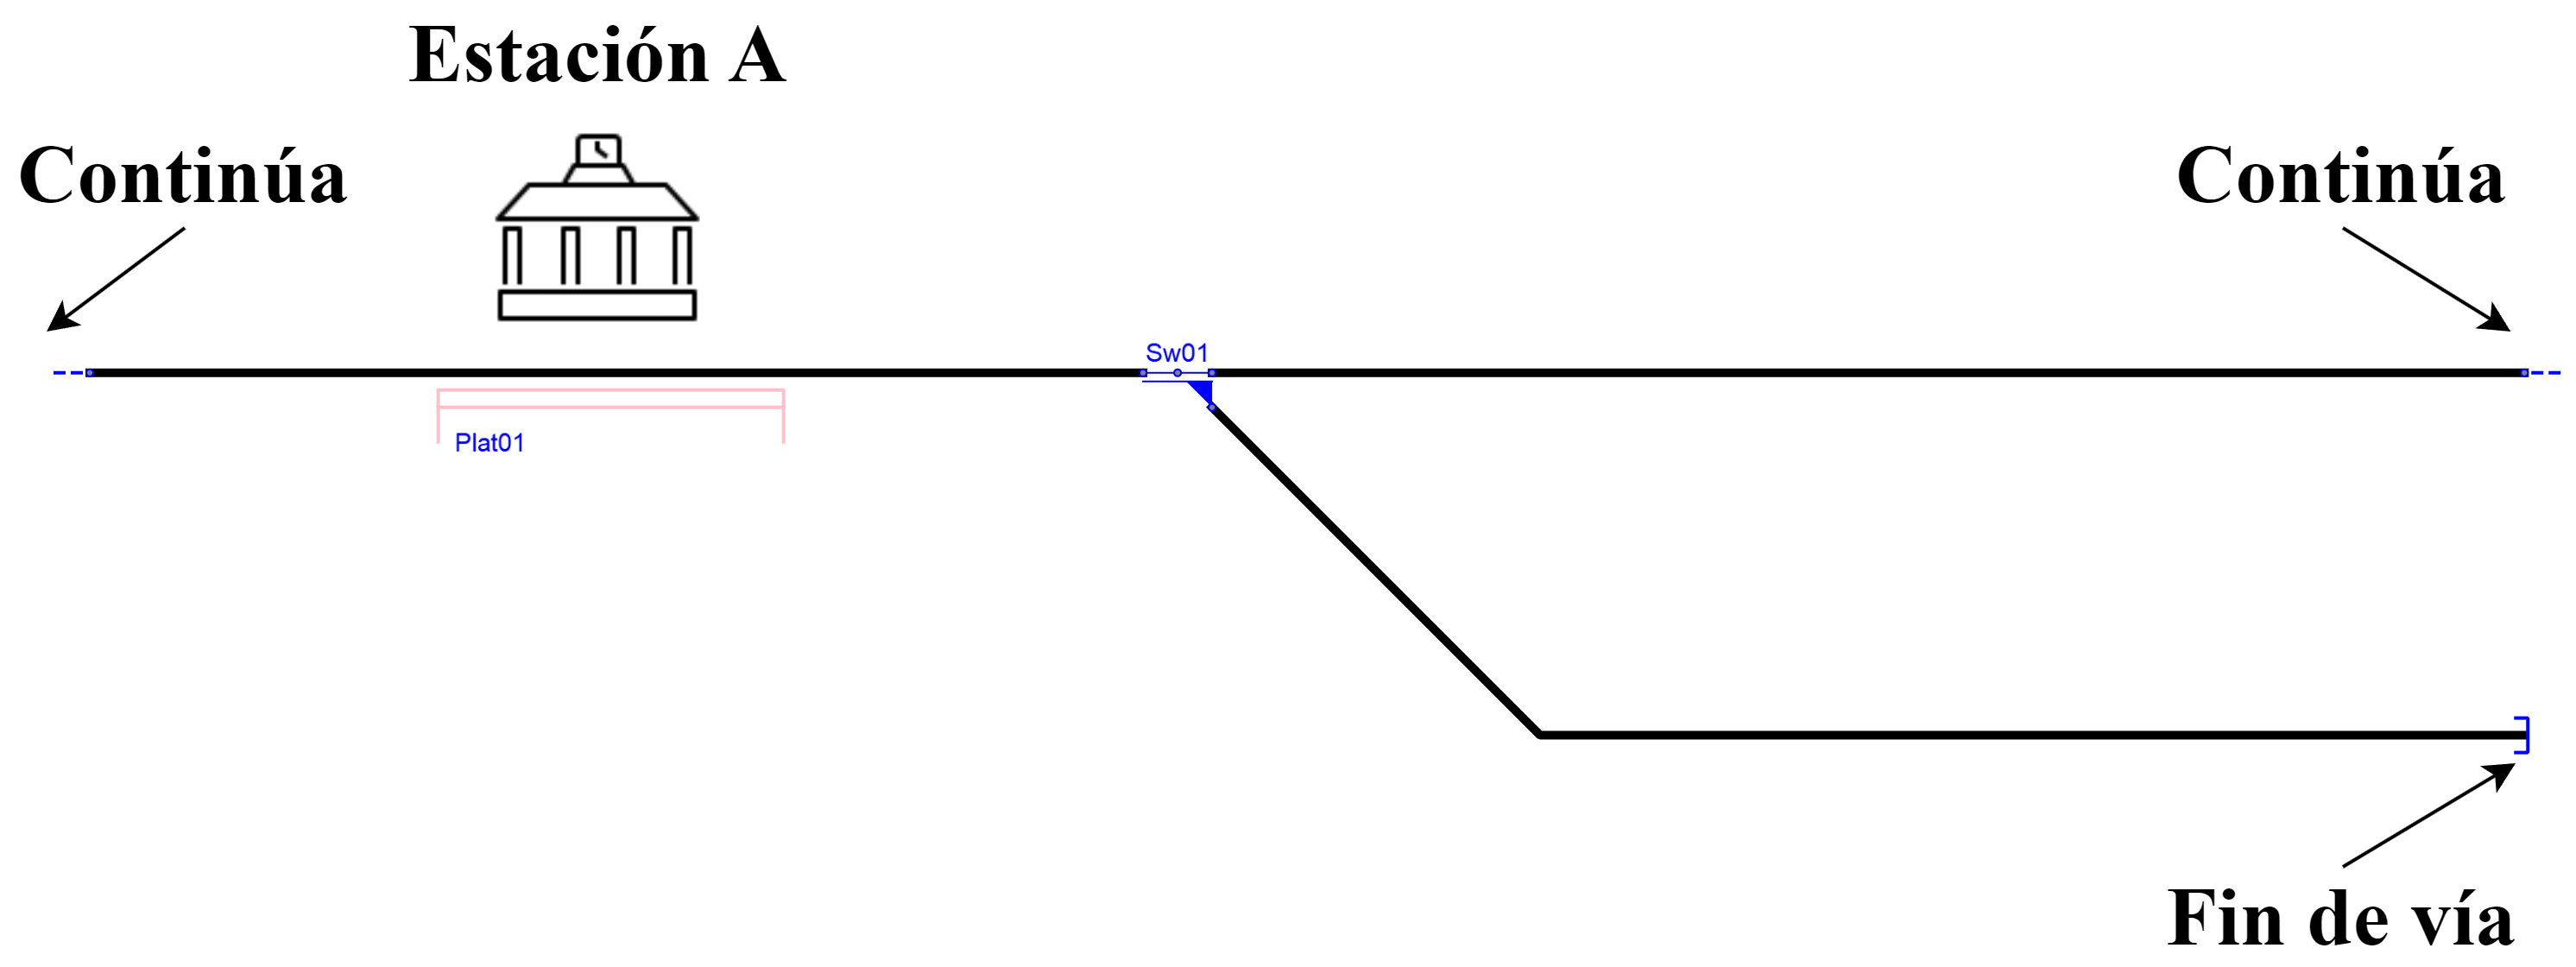
\includegraphics[width=0.9\textwidth]{Figuras/Border.png}
        \centering\caption{Topología de ejemplo con finales de vía relativos y absolutos.}
        \label{fig:frontera_1}
    \end{figure}

    Un ejemplo de fin de vía relativo sería la frontera entre las estaciones A y B. Las vías continúan a la derecha de A, pero no son parte del alcance del sistema que controla los elementos ferroviarios en las inmediaciones de A. En tanto que un fin de vía absoluto sería todo final literal de la red ferroviaria, tales como terminales, talleres y vías secundarias sin retorno, como la ramificación saliente de la vía principal.
    
    Un fin de vía relativo es todo aquel límite que define el alcance del sistema de señalamiento, pero no necesariamente es el final de la red. Es decir, el sistema podrá recibir información de cualquier sensor dentro de estos límites, o incluso de algunos sensores en la frontera exterior, pero solo podrá comandar los actuadores dentro de la zona. Esto es de vital importancia a la hora de reducir la complejidad de la red, al realizar el procesamiento de forma distribuida, sin depender de un decisión centralizada.

    Este elemento ferroviario es modelo por la clase border, cuyo ejemplo se visualiza en el Código \ref{lst:lineBorder}. Siempre se definen referido a un único netElement, en este caso el netElement ne114 y a una coordenada intrínseca que puede ser 0 si se encuentra al principio del netElement, o de 1 si se encuentra al final.

    \begin{lstlisting}[language = XML, caption = Clase border , label = {lst:lineBorder}]
    <border isOpenEnd="false" externalRef="" type="station" id="sb540">
        <designator register="_Example" entry="BORDER SB05"/>
        <spotLocation netElementRef="ne114" intrinsicCoord="0.0000" applicationDirection="reverse" id="sb540_sloc01"/>
        <name name="SB05" language="en"/>
    </border>
    \end{lstlisting}

    Un fin de vía absoluto es todo aquel límite que define el final físico del tendido ferroviario, luego del cual ya no se tiene infraestructura. Podemos encontrar estos límites en los talleres ferroviarios, en las terminales principales de cada red o en vías utilizadas para estacionar los trenes por fuera de la rama principal en uso. Estos límites deben estar adecuadamente protegidos y señalizados.

    Este elemento ferroviario es modelo por la clase bufferStop, cuyo ejemplo se visualiza en el Código \ref{lst:bufferStop}. Al igual que la clase border, se definen referido a un único netElement, en este caso el netElement ne3 y a una coordenada intrínseca que puede ser 0 si se encuentra al principio del netElement, o de 1 si se encuentra al final.
    
    \begin{lstlisting}[language = XML, caption = Clase bufferStop , label = {lst:bufferStop}]
    <bufferStop type="fixedBufferStop" id="bus5">
        <designator register="_Example" entry="BUFFERSTOP Buf05"/>
        <spotLocation netElementRef="ne3" intrinsicCoord="0.0000" applicationDirection="reverse" id="bus5_sloc01"/>
        <name name="Buf05" language="en"/>
    </bufferStop>
    \end{lstlisting}
    \subsection{Sistemas de detección de formaciones ferroviarias}
    \label{sec:detectors}
    
    Es de vital importancia que el sistema pueda determinar la posición de un tren dentro del tendido ferroviario. De esta manera, poder habilitar la circulación en secciones donde no exista peligro de colisión con otros formaciones o, por el contrario, detener la marcha de las formaciones anteriores para evitar accidentes. Existen diversas maneras de detectar la posición de un tren, entre ellas el uso de circuitos de vía y contadores de ejes (Figura \ref{fig:deteccion_1}). 

    \begin{figure}[H]
        \centering
        \includegraphics[width=1\textwidth]{Figuras/detector}
        \centering\caption{Circuito de vía (01) y contador de ejes (AxC01).}
        \label{fig:deteccion_1}
    \end{figure}

    Los circuitos de vía (Figura \ref{fig:deteccion_2}) son dispositivos eléctricos que aplican una diferencia de potencial entre los rieles. Cuando una formación ingresa a la sección, sus ruedas metálicas cortocircuitan ambos rieles. El cortocircuito es detectado por el relé, que a su vez, reporta el estado al resto del sistema. 

    \begin{figure}[H]
        \centering
        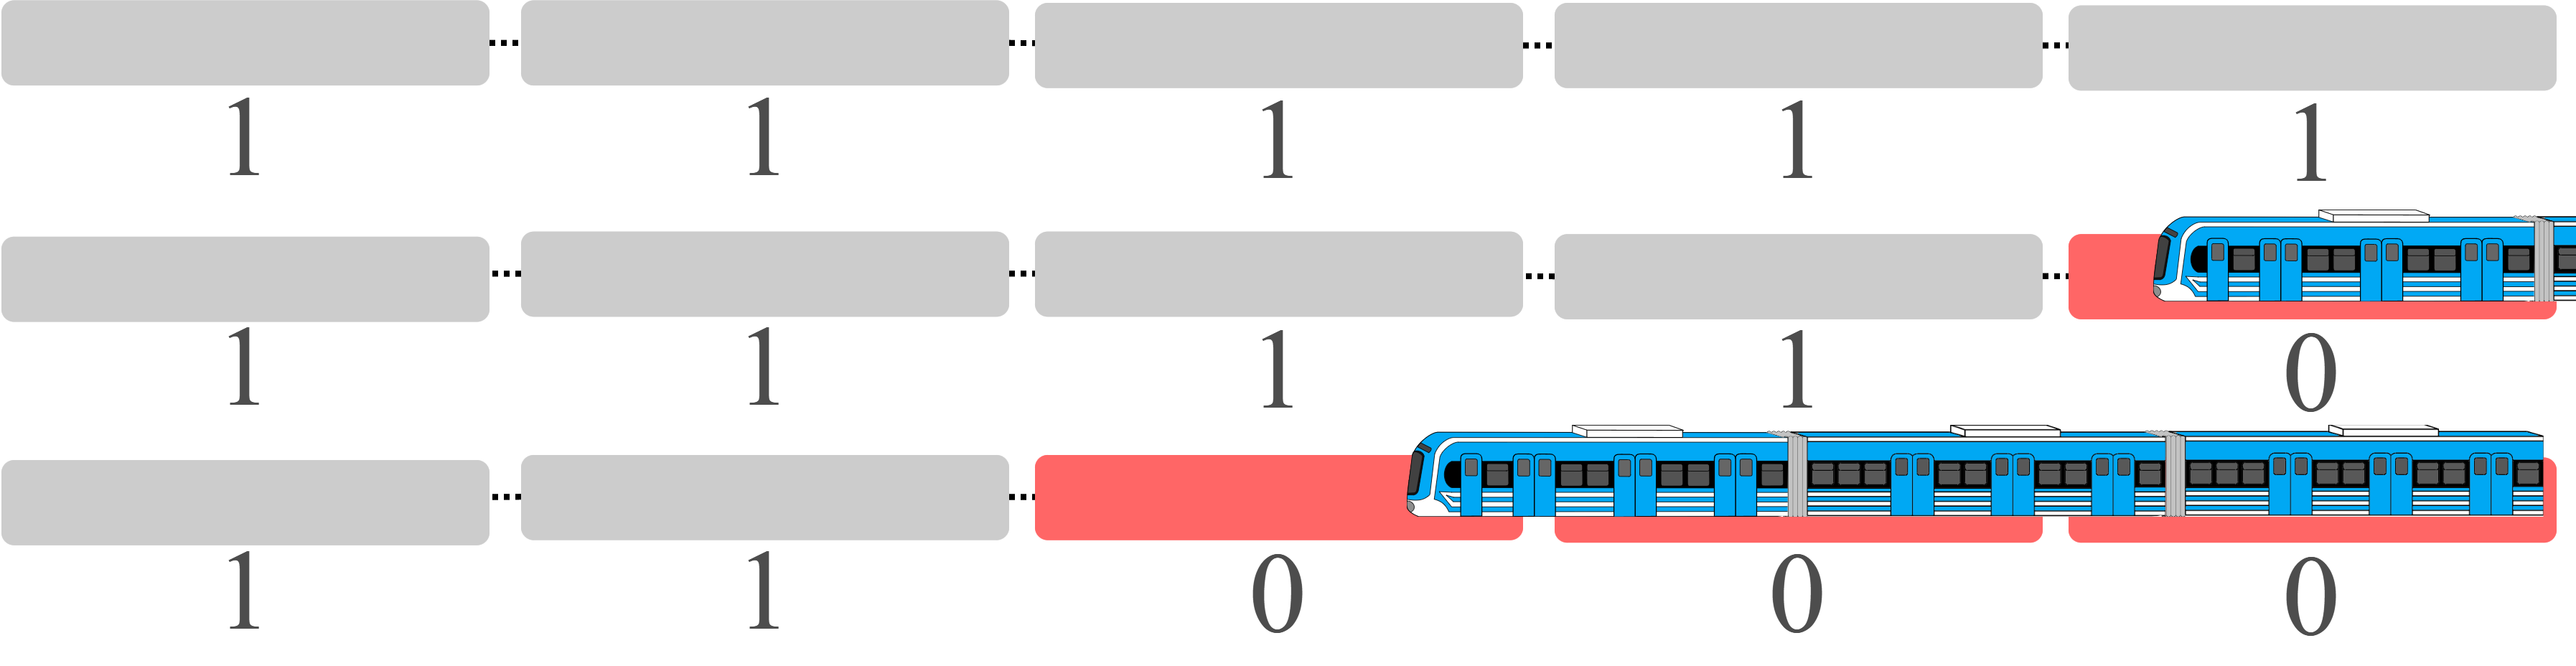
\includegraphics[width=1\textwidth]{Figuras/circuitoVia}
        \centering\caption{Circuito de vía libre y ocupado.}
        \label{fig:deteccion_2}
    \end{figure}

    En caso de que la alimentación se interrumpa, el cableado sufra alguna falla, vandalismo, inundación, o que efectivamente una formación ocupe la sección, el circuito de vía reportará que la sección se encuentra ocupada. De esta manera, solo es posible recibir un reporte de sección desocupada cuando la sección efectivamente se encuentre desocupada. A este principio se le denomina fail-safe \cite{Paper_5,Paper_94,Paper_95,Paper_96}. Es decir, si por alguna razón algo falla, el sistema adopta la condición más restrictiva, mitigando la posibilidad de una situación peligrosa. 
    
    Existe una discontinuidad entre los rieles denominado juntura, que permite la expansión de los mismos al ser sometidos a altas temperaturas sin que los rieles se doblen y provoquen daños a la infraestructura. Los circuitos de vía, se relacionan directamente a las junturas entre las vías, modelados por la clase \textit{railJoint} en railML.  Esta discontinuidad eléctrica es lo que limita la acción del circuito de vía a la región entre dos junturas.

    En el código \ref{lst:trackCircuit} podemos ver un ejemplo de la clase \textit{tvdSection} dentro de la clase \textit{interlocking}, que incluye a la clase \textit{assetsForIL} y estos, a su vez, a la clase vector de \textit{tvdSections}. Esta clase posee un id (tvd7), la tecnología utilizada (en este caso \textit{trackCircuit}, circuito de vía) y los límites donde el circuito de vía es válido: los \textit{bufferStop} bus1 y bus2.

    \begin{lstlisting}[language = XML, caption = Clase \textit{TrackCircuit} , label = {lst:trackCircuit}]
    <tvdSection id="tvd7" partialRouteReleaseDelay="PT4S" residualRouteCancellationDelay="PT90S" technology="trackCircuit" isBerthingTrack="false">
        <designator register="Example" entry="01"/>
        <hasDemarcatingBufferstop ref="bus2"/>
        <hasDemarcatingBufferstop ref="bus1"/>
    </tvdSection>
    \end{lstlisting}

    Los sistemas contadores de ejes (Figura \ref{fig:deteccion_2}) consisten en sensores pasivos instalados en la cara interna de unos de los rieles y un sistema externo de procesamiento de datos. Estos sistemas no dependen de la aplicación de tensiones en la vía. Además, no solo permiten detectar la presencia de una formación, sino que también pueden usarse para medir la integridad de la formación, si se conoce a priori la cantidad de ejes de la misma. 

    \begin{figure}[H]
        \centering
        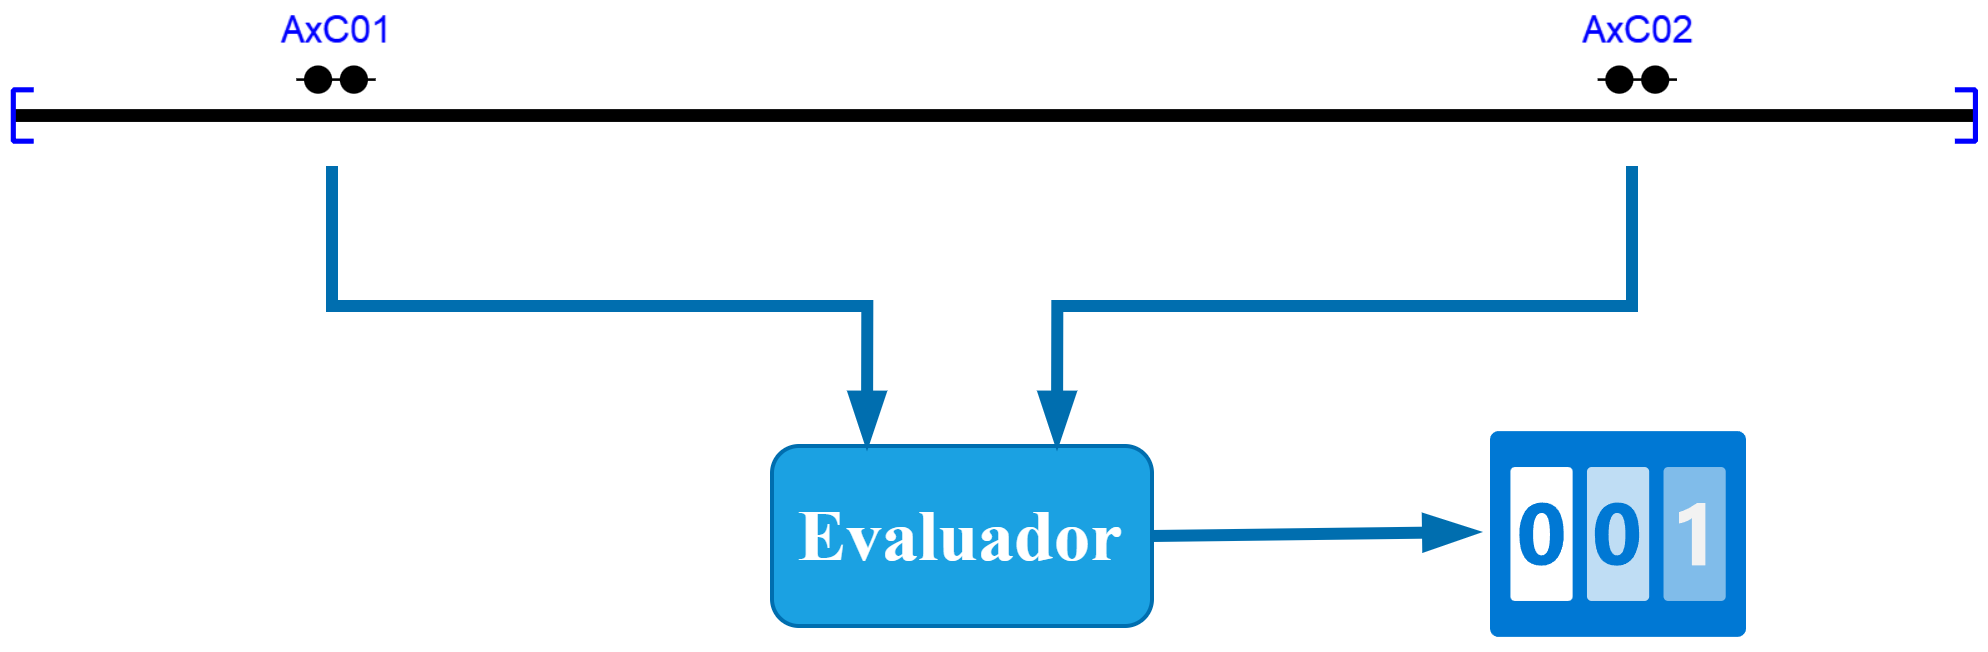
\includegraphics[width=1\textwidth]{Figuras/contador}
        \centering\caption{Contadores de ejes.}
        \label{fig:deteccion_2}
    \end{figure}

    Al igual que los circuitos de vía, los sistemas contadores de eje siguen el principio de fail-safe, adoptando la condición mas restrictiva en caso de falla. Ambos sistemas pueden utilizarse en simultáneo, de ser requerido. En el código \ref{lst:axleCounter} podemos ver un ejemplo de la clase \textit{trainDetectionElement}, dentro de la clase \textit{functionalInfrastructure}, dentro de la clase \textit{infrastructure}. En este ejemplo la bclase fue definida como tipo \textit{axleCounter} (contador de eje) y se le asigna el nombre AxC01 que vemos en la Figura \ref{fig:deteccion_1}, referido al \textit{netElement} ne1. También podemos ver que este contador de ejes se activa en ambos sentidos (applicationDirection = both) y su coordenada intrínseca dentro del \textit{netElement} ne1, dentro de los dos tercios de la sección.

    \begin{lstlisting}[language = XML, caption = Clase \textit{TrainDetectionElement} , label = {lst:axleCounter}]
    <trainDetectionElement id="ac6" type="axleCounter">
        <name name="AxC01" language="en"/>
        <spotLocation id="ac6_sloc01" netElementRef="ne1" applicationDirection="both" intrinsicCoord="0.6710"/>
        <designator register="Example" entry="TRAIN DETECTION ELEMENT AxC01"/>
    </trainDetectionElement>
    \end{lstlisting}
    \subsection{Automatic Train Stop (ATS)}

\lipsum[1]

    \begin{figure}[!h]
        \centering
        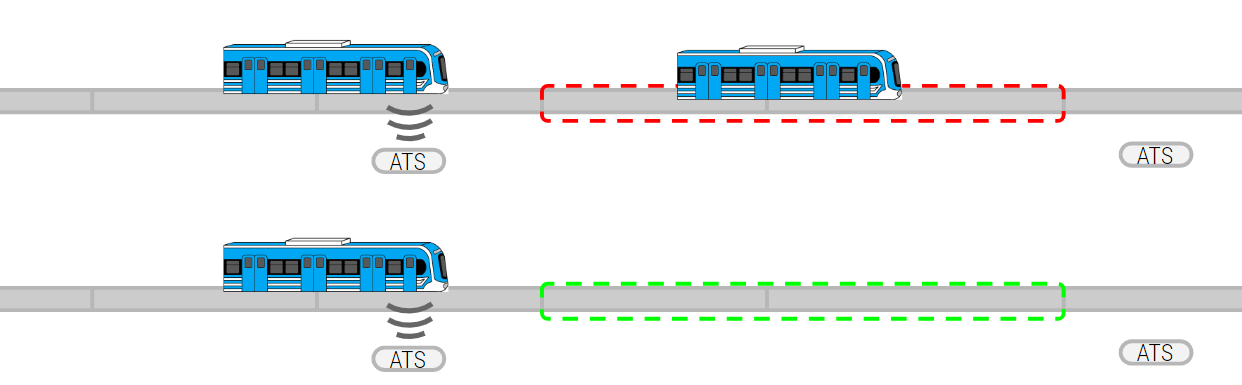
\includegraphics[width=1\textwidth]{Figuras/ATS}
        \centering\caption{ATS.}
        \label{fig:ATS_1}
    \end{figure}

\lipsum[1]
    \subsection{Estaciones ferroviarias}
    \label{sec:platform}
    
    Las estaciones ferroviarias son las zonas donde las formaciones pueden detenerse para que los pasajeros puedan descender y nuevos pasajeros puedan abordar. En función del tamaño de las formaciones y la geografía del lugar, las plataformas desde donde ascienden y descienden los pasajeros pueden estar elevadas con respecto al suelo o a ras del mismo. El largo de las plataformas también depende de la cantidad de coches de las formaciones.
    
    Como puede verse en la Figura \ref{fig:estacion_1}, las estaciones ferroviarias incluyen no solo a las plataformas, sino que también pueden centralizar el control de varias operaciones logísticas como la asignación de rutas. No obstante, en este trabajo nos referiremos a las estaciones como plataformas indistintamente.
    
        \begin{figure}[H]
            \centering
            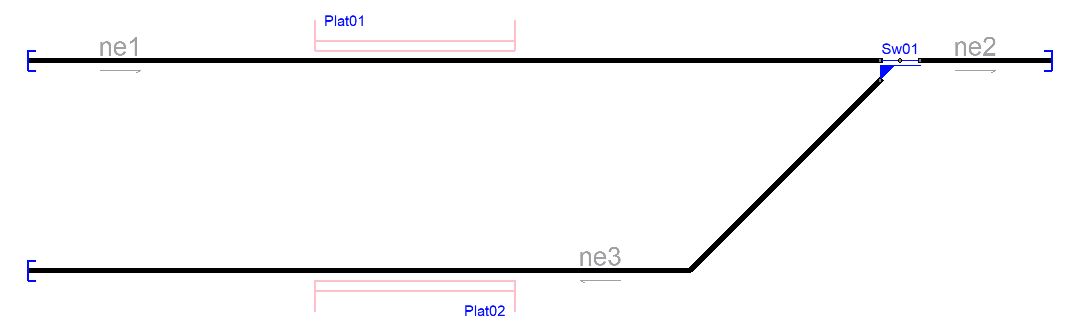
\includegraphics[width=1\textwidth]{Figuras/Platform.png}
            \centering\caption{Estación de doble plataforma.}
            \label{fig:estacion_1}
        \end{figure}
    
    Las estaciones de mayor complejidad o de mayor convergencia de ramales suelen concentrar el control de la estación donde se encuentran y varias estaciones vecinas. Las estaciones terminales, a menudo, pueden incluso tener control total de varios ramales completos.

    En el Código \ref{lst:platform_1} se pueden ver la implementación de la clase platform de las plataformas ilustradas en la Figura \ref{fig:estacion_1}. Esta clase se encuentra dentro de la clase infrastructure, que a su vez contiene a la clase functionalInfrastructure. La misma incluye atributos como la altura, el nombre asignado que se visualiza en la Figura \ref{fig:estacion_1} y el netElement al que se encuentran asociadas cada una de las plataformas.

    \begin{lstlisting}[language = XML, caption = Clase Platform , label = {lst:platform_1}]
    <platforms>
        <platform id="plf3" height="0">
            <name name="Plat01" language="en"/>
            <linearLocation id="plf3_lloc01" applicationDirection="both">
                <associatedNetElement keepsOrientation="true" netElementRef="ne1"/>
            </linearLocation>
            <designator register="_Example" entry="PLATFORM Plat01"/>
            <length type="physical" value="0" validForDirection="both"/>
        </platform>
        <platform id="plf6" height="0">
            <name name="Plat02" language="en"/>
            <linearLocation id="plf6_lloc01" applicationDirection="both">
                <associatedNetElement keepsOrientation="true" netElementRef="ne3"/>
            </linearLocation>
            <designator register="_Example" entry="PLATFORM Plat02"/>
            <length type="physical" value="0" validForDirection="both"/>
        </platform>
    </platforms>
    \end{lstlisting}

    Los datos relativos a la características físicas como el largo y el ancho la encontramos dentro de la clase visualization, dentro de la clase infrastructureVisualizations, como se puede ver en el Código \ref{lst:platform_2}.

    \begin{lstlisting}[language = XML, caption = Clase visualization , label = {lst:platform_2}]
    <spotElementProjection refersToElement="plf3" id="vis01_sep4">
        <name name="Plat01" language="en"/>
        <coordinate x="-125.455" y="-240.000"/>
    </spotElementProjection>
    <spotElementProjection refersToElement="plf6" id="vis01_sep5">
        <name name="Plat02" language="en"/>
        <coordinate x="-125.454" y="-30.000"/>
    </spotElementProjection>
    \end{lstlisting}

    Conocer las dimensiones del elemento físico que representa esta clase es fundamental a la hora de analizar el impacto de este elemento en la red y donde se deberían asignar las señales ferroviarias.
    \subsection{Cruces ferroviarios}

Los cruces ferroviarios son la intersección entre la vía ferroviaria y una ruta vehicular o peatonal. Estos cruces pueden ser bajo nivel (túnel por debajo de la vía), sobre nivel (puente vehicular por sobre la vía) o a nivel. Un paso a nivel es una zona muy crítica del sistema ferroviario, ya que, a diferencia de un paso sobre nivel o bajo nivel, conviven simultáneamente la formación y el transito vehicular y peatonal. En la Figura \ref{fig:cruce_1} se ilustra la intersección entre el tendido ferroviario, un cruce vehicular y un cruce peatonal.

    \begin{figure}[!h]
        \centering
        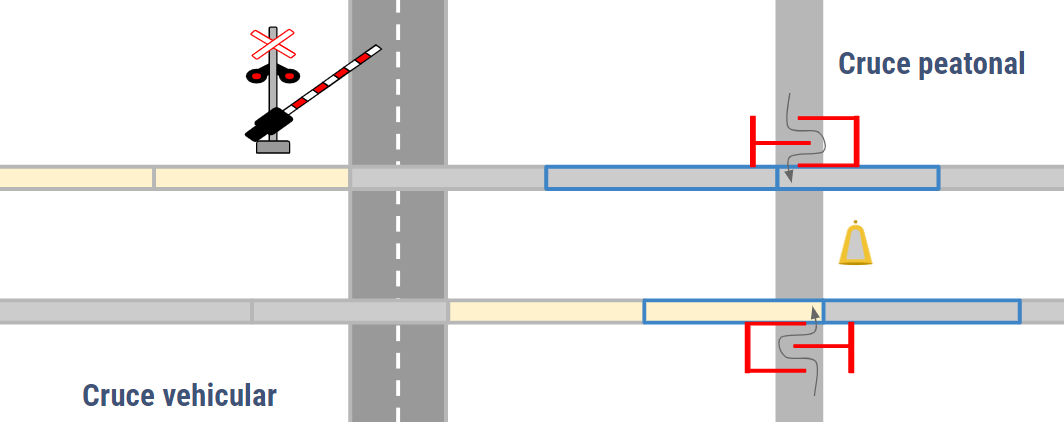
\includegraphics[width=1\textwidth]{Figuras/cruce}
        \centering\caption{XXXXX.}
        \label{fig:cruce_1}
    \end{figure}
    
Los pasos a nivel peatonales incluyen un pequeño laberinto zigzagueante para forzar al peatón a aminorar su marcha y ver a ambos lados antes de cruzar las vías. A menudo suelen estar acompañados de indicaciones lumínicas y sonoras que se accionan tan pronto el tren se encuentre dentro de un rango de varios metros cercano al paso a nivel.

Los pasos a nivel vehiculares añaden barreras ferroviarias para detener el tráfico vehicular cuando un tren se encuentra dentro de un rango de seguridad definido.  El sistema de control de la barrera mantiene el brazo de esta en alto para permitir la circulación vehicular. Si un tren es detectado cerca del paso a nivel, se desenergiza la barrera y comienza a descender el brazo por efecto de la gravedad. Solo cuando la barrera baja, el tren tiene permitido avanzar sobre el cruce, siendo el paso a nivel un sector de altísimo riesgo. Al desocuparse las secciones próximas al paso a nivel, la barrera vuelve a energizarse y se sitúa en estado alto nuevamente, a la espera de otro tren para reiniciar el proceso. 

Se debe destacar que el mismo proceso de descenso de la barrera ocurrirá si esta se desenergiza por una falla electricomecánica y/o pérdida de alimentación. Es decir, el sistema asumirá el estado más seguro ante cualquiera de los mencionados fallos, siguiendo el principio de falla segura.
    \subsection{Máquina de cambios}
    \label{sec:switches}
 
    Una máquina de cambios (Figura \ref{fig:cambios_1}) es un mecanismo utilizado para permitir el paso de las formaciones de una vía a una ramificación del recorrido principal. Esto se realiza mediante el movimiento de la aguja del cambio (riel móvil) hacia su respectiva contraaguja (riel fijo) hasta obtener un adecuado acoplamiento que permita la circulación de la formación.

    \begin{figure}[!h]
        \centering
        \includegraphics[width=0.9\textwidth]{Figuras/Cambios.jpg}
        \centering\caption{Máquina de cambios.}
        \label{fig:cambios_1}
    \end{figure}

    En la Figura \ref{fig:cambios_2} se muestra el cambio de vía de la estación Matheu de la Línea Mitre. Se observa que según sea la posición de la máquina de cambios, el tren puede continuar en la misma vía o hacer el cambio a la otra vía.

    \begin{figure}[!h]
        \centering
        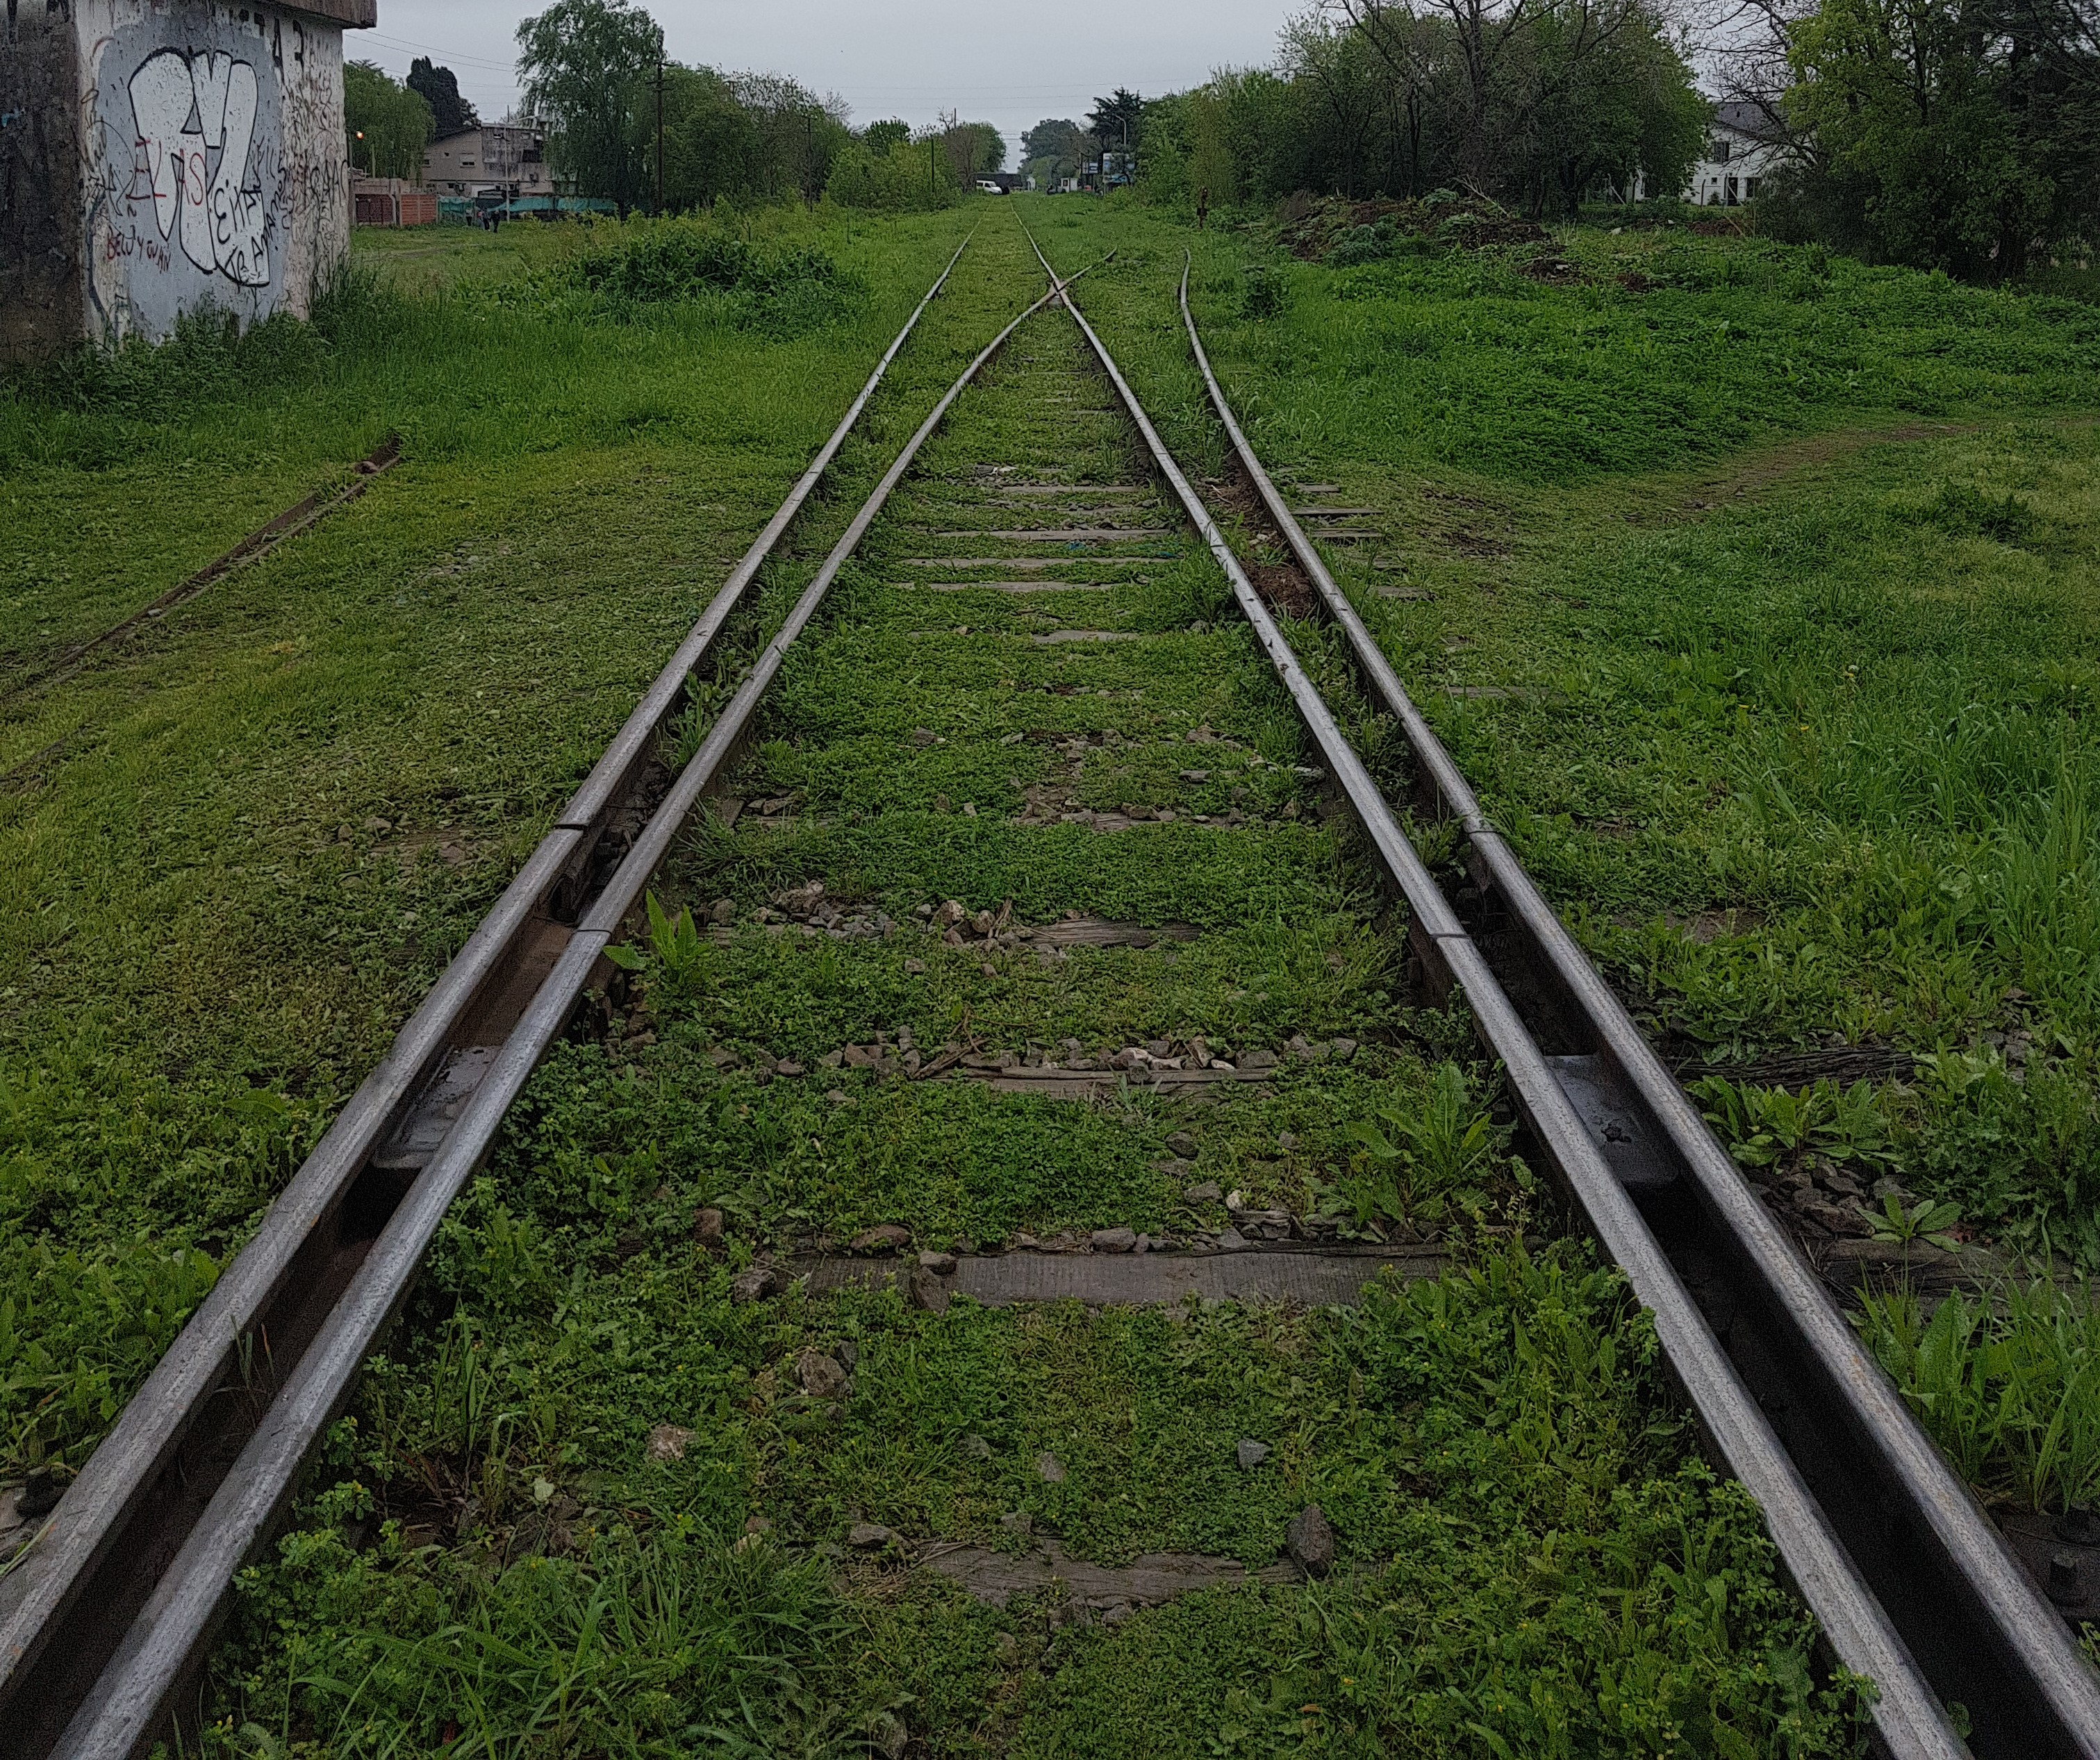
\includegraphics[width=0.9\textwidth]{Figuras/Cambios_2.jpg}
        \centering\caption{Cambio de vías de estación Matheu, Linea Mitre.}
        \label{fig:cambios_2}
    \end{figure}

    En la Figura \ref{fig:cambios_3} se muestran las posiciones que puede adoptar el cambio. En la posición normal, los trenes pueden circular de forma directa, en paralelo, por la vía principal en sentidos opuestos. En la posición reversa, en cambio, se permite el intercambio de trenes de una rama principal a otra en sentido opuesto o a una ramificación secundaria de la red.

    \begin{figure}[!h]
        \centering
        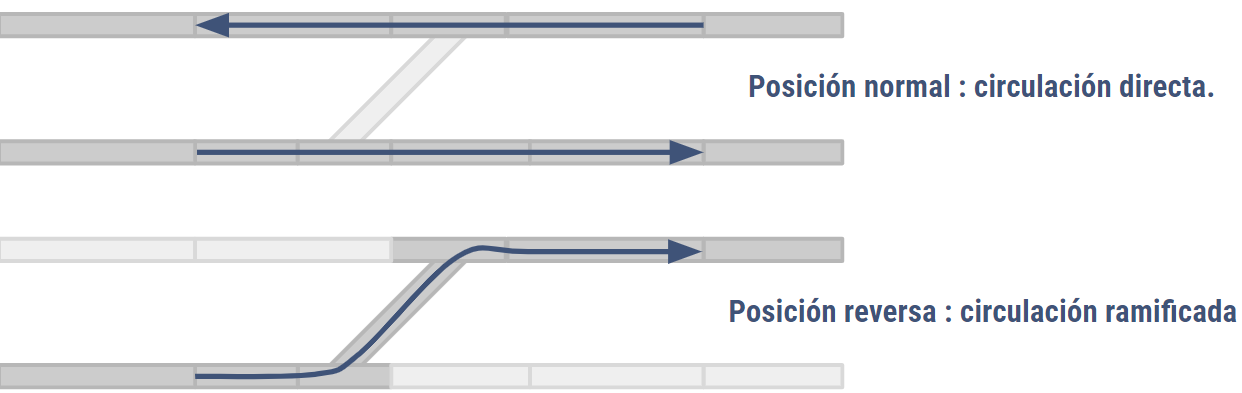
\includegraphics[width=0.9\textwidth]{Figuras/cambio_3.PNG}
        \centering\caption{Posiciones adoptadas por una máquina de cambios simple.}
        \label{fig:cambios_3}
    \end{figure}

    Las máquinas de cambios son un elemento activo de la red ferroviaria, controlados por el sistema de enclavamientos. Al ser mecanismos que necesitan tiempo para cambiar de un estado al otro, no puede asumirse que el comando es obedecido al instante. Incluso podría darse el caso que jamás llegue a cumplirse la orden debido a desperfectos mecánicos o eléctricos. Es por eso que introducimos los conceptos de comando, indicación y correspondencia, tal como se ilustran en la Figura \ref{fig:cambios_4}.

    \begin{figure}[!h]
        \centering
        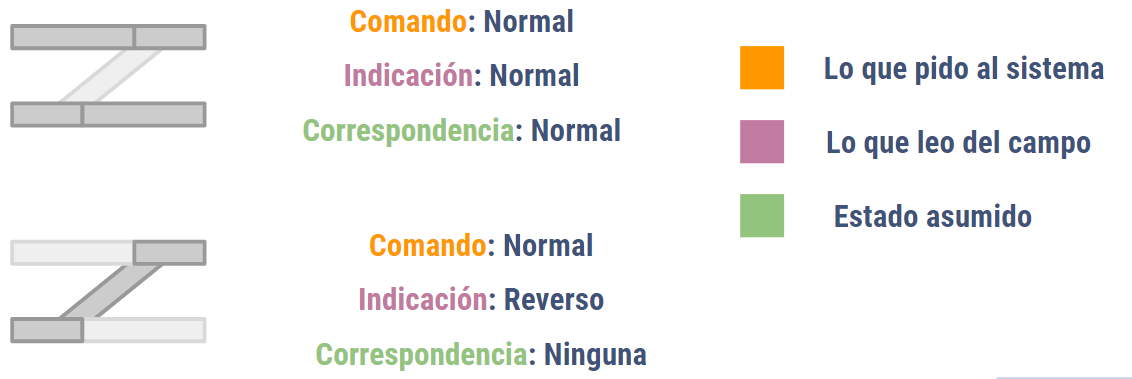
\includegraphics[width=1\textwidth]{Figuras/cambios}
        \centering\caption{Comando, indicación y correspondencia en máquinas de cambios.}
        \label{fig:cambios_4}
    \end{figure}
    
    El comando es la instrucción que el sistema de enclavamientos envía a la máquina de cambios. Esta instrucción puede ser modificar la posición de normal a reverso o de reverso a normal. La indicación es el estado que la máquina de cambios informa al sistema de enclavamientos. El sistema solo asume que el comando fue obedecido cuando tanto el comando como la indicación muestran una correspondencia. En caso contrario, el sistema de enclavamiento no puede asumir cual es el estado real del sistema, si el comando enviado o el estado reportado por la máquina de cambios. El mismo concepto puede ser aplicado en cualquier otro elemento mecánico, como por ejemplo las barreras ferroviarias.

    El RNA debe analizar diversos atributos distribuidos entre la clase switchIS (Código \ref{lst:switchIS}), la clase spotElementProjection (Código \ref{lst:switch}) y switchIL (Código \ref{lst:switchIL}). La clase switchIS se encuentra dentro del vector de clases switchesIS, dentro de functionalInfrastructure, que a su vez es parte de la clase infrastructure. La clase define el id de la máquina de cambios, el tipo (ordinario), el netElement al cual pertenece la entrada del cambio y hacia que lado se encuentra la vía de continuación y ramificación si transitamos desde el netElement del cambio hacia el cambio mismo. En este caso, si transitamos por el netElement ne16 el tren tendrá la vía de continuación en la mano derecha y la ramificación en la mano izquierda. Las máquina de cambio ordinarias siempre tienen una rama izquierda y una rama derecha definida. Además, dentro de la definición de cada rama tenemos el atributo netRelationRef, del cual se puede obtener, procesamiento mediante, los otros netElement correspondientes a las ramas: ne15 y ne14.

    \begin{lstlisting}[language = XML, caption = Clase switchIS , label = {lst:switchIS}]
    <switchIS id="swi84" continueCourse="right" branchCourse="left" type="ordinarySwitch">
        <name name="Sw01" language="en"/>
        <spotLocation id="swi84_sloc01" netElementRef="ne16" applicationDirection="reverse" intrinsicCoord="0.0000"/>
        <designator register="_Example" entry="SWITCH Sw01"/>
        <leftBranch netRelationRef="nr_ne15ne16_swi84" branchingSpeed="0" joiningSpeed="0" radius="-500"/>
        <rightBranch netRelationRef="nr_ne14ne16_swi84" branchingSpeed="0" joiningSpeed="0" radius="0"/>
    </switchIS>
    \end{lstlisting}

    La clase spotElementProjection define la ubicación en el espacio del elemento ferroviario referido. En este caso, como se puede ver en el Código \ref{lst:switch}, la posición de la máquina de cambios es la coordenada (-561 ; -450).

    \begin{lstlisting}[language = XML, caption = Clase spotElementProjection , label = {lst:switch}]
    <spotElementProjection refersToElement="swi84" id="vis01_sep16">
        <name name="Sw01" language="en"/>
        <coordinate x="-560.994" y="-450.000"/>
    </spotElementProjection>
    \end{lstlisting}

    La clase switchIL, definida dentro del vector de clases switchesIL, se encuentra dentro de la clase assetsForIL, en la clase interlocking. Contiene datos extra sobre el comportamiento dinámico de la máquina de cambios y define explícitamente los otros dos nodos, en contraposición a switchIS del cual hay que obtenerlos procesando un string. El RNA puede obtener los netElement de ambas clases y compararlos, anulando el análisis si los netElement definidos en switchIS y switchIL no son coincidentes.
    
    \begin{lstlisting}[language = XML, caption = Clase switchIL , label = {lst:switchIL}]
    <switchIL id="il_swi84" maxThrowTime="PT10S" typicalThrowTime="PT6S" isKeyLocked="false" returnsToPreferredPosition="false">
        <refersTo ref="swi84"/>
        <branchLeft ref="ne15"/>
        <branchRight ref="ne14"/>
    </switchIL>
    \end{lstlisting}
    
    El RNA utiliza el Algoritmo \ref{alg:switches} para detectar todos estos parámetros y crear un vector de máquinas de cambios (switches) indexado por el id de cada máquina de cambios (sw\_id). La existencia y ubicación de las máquinas de cambios ya se habían obtenido mediante el análisis de la red de grafos ferroviaria. El Algoritmo \ref{alg:switches} analiza la clase switchIS y confirma la existencia de la máquina de cambios, para luego la clase spotElementProjection y confirmar la ubicación de la misma. Los datos obtenidos en switches[sw\_id].LeftBranch y switches[sw\_id].RightBranch, permiten obtener los nodos de las ramificaciones que luego se conformarán analizando la clase switchIL en algoritmos posteriores.

    \begin{algorithm}\captionsetup{labelfont={sc,bf}, labelsep=newline}
            \caption{Algoritmo detector de máquinas de cambios.}
            \label{alg:switches}
            \begin{algorithmic}
                \STATE \{switches\} $\gets$ \{\}
                \IF {infrastructure.SwitchesIS != None} 
                    \FOR{i in infrastructure.SwitchesIS[0].SwitchIS}
                        \IF{i.Id not in switchesIS.keys()}
                            \STATE sw\_id $\gets$ i.Name[0].Name
                            \STATE j $\gets$ i.SpotLocation[0]
                            \STATE left\_id $\gets$ i.LeftBranch[0].NetRelationRef
                            \STATE right\_id $\gets$ i.RightBranch[0].NetRelationRef
                            \STATE switches[sw\_id] $\gets$ \{"Node":j.NetElementRef\}
                            \STATE switches[sw\_id] $\gets$ \{"Continue":i.ContinueCourse\}
                            \STATE switches[sw\_id] $\gets$ \{"Branch":i.BranchCourse\}
                            \STATE switches[sw\_id] $\gets$ \{"Dir":j.ApplicationDirection\}
                            \STATE switches[sw\_id] $\gets$ \{"LeftBranch":j.left\_id\}
                            \STATE switches[sw\_id] $\gets$ \{"RightBranch":j.right\_id\}
                        \ENDIF
                    \ENDFOR
                \ENDIF
                \STATE visual\_data $\gets$ visualization.Visualization
                \IF {visual\_data != None}
                    \FOR {i in  visual\_data[0].SpotElementProjection}
                        \STATE sw\_id $\gets$ i.Name[0].Name
                        \IF {'Sw' in sw\_id}
                            \STATE pos\_x $\gets$ int(i.Coordinate[0].X)
                            \STATE pos\_y $\gets$ int(i.Coordinate[0].Y)
                            \STATE switches[sw\_id] $\gets$ \{"Position":[pos\_x,-pos\_y]\}
                        \ENDIF 
                    \ENDFOR
                \ENDIF
            \OUTPUT switchesIS
            \end{algorithmic}
        \end{algorithm}
    
    % SEMAFOROS
    \subsection{Señales ferroviarias}

El sistema de señalamiento utiliza los semáforos ferroviarios (en adelante denominados señales) para indicarle al conductor del tren si tiene autoridad de tránsito en al próximo tramo de vías y a qué velocidad se le permite circular; esto, por medio del color del semáforo, denominado aspecto. A diferencia de los semáforos vehiculares, en los que cada color es alternado por otro de la secuencia rojo-amarillo-verde en función del tiempo, los semáforos ferroviarios cambian su aspecto en función de los eventos de los tramos siguientes. En la Figura \ref{fig:signal_1} se presenta un esquema de señales de tres aspectos, que es el tipo de semáforo que se utiliza en la gran mayoría de las líneas ferroviarias.

    \begin{figure}[!h]
        \centering
        \includegraphics[width=1\textwidth]{example-image}
        \centering\caption{XXXXX.}
        \label{fig:signal_1}
    \end{figure}

Otra diferencia fundamental es que no todos los semáforos ferroviarios poseen tres aspectos. Los semáforos de maniobras constan de solo dos, amarillo (precaución) y rojo (prohibido avanzar), y algunas líneas, como la Línea Roca, utilizan semáforos de cuatro aspectos. En la Figura \ref{fig:signal_2} se visualizan los semáforos de dos aspectos. Se utilizan en cambios de vías donde, por su peligrosidad, solo se podrían permitir aspectos rojos y amarillos.

    \begin{figure}[!h]
        \centering
        \includegraphics[width=1\textwidth]{example-image}
        \centering\caption{XXXXX.}
        \label{fig:signal_2}
    \end{figure}

Los semáforos de cuatro aspectos son utilizados en la Línea Roca y poseen un doble amarillo antes del amarillo simple, para permitir así tramos de vías más cortos de forma segura. Como no son objeto de estudio del presente trabajo, no serán explicados aquí. (EDITAR)

    \begin{figure}[!h]
        \centering
        \includegraphics[width=1\textwidth]{example-image}
        \centering\caption{XXXXX.}
        \label{fig:signal_3}
    \end{figure}

EXPLICAR MAS LOS SEMAFOROS.
\section{Algoritmos de generación de señalamiento}
    \label{sec:generacion}
\lipsum[1]

\subsection{Señalización en fin de vía y transiciones}
    
	\label{sec:sig_border}
    
    % Autoridad > derecho limitado a una porcion
    % Claridad > autoridad no ambigua
    % Anticipacion > avisar con antelacion
    % Granularidad > rutas cortas y funcionales
    % Terminalidad > avisar fin de via
    % Infraestructura > avisar de infraestructura
    % No bloqueo > circulacion fluida

    Tal como se definió en la Sección \ref{sec:bufferstop}, las redes ferroviarias presentan tanto fines de vía absolutos (modelados en railML por la clase \textit{bufferStop}) como fines de vía relativos (modelados en railML por la clase \textit{lineBorder}). El RNA detecta estos elementos y generará el señalamiento correspondiente en base a los principios de señalamiento expuestos en la Sección \ref{sec:principios}.

    En el caso de las transiciones para fines de vía relativos, por el principio de infraestructura ($P_6$), es necesario que existan señales que indiquen que la formación pueda circular por la transición de una región ferroviaria a otra. Esta señal debe otorgar autoridad a la formación de forma unívoca, por el principio de claridad ($P_2$). Adicionalmente, esa señal debe situarse con suficiente antelación a la transición, por el principio de anticipación ($P_3$). Aplicando el principio de no bloqueo ($P_7$) regulamos la circulación entre dos regiones ferroviarias para que puedan circular sin demoras ni atascos. Finalmente, el principio de granularidad ($P_4$) y autoridad ($P_1$) nos pide que el derecho de uso de la infraestructura debe ser acotado, pero funcional. Es decir, la autoridad debe aplicarse en una sección con un mínimo de largo como para que tenga sentido. 

    En el Algoritmo \ref{alg:lineBorder} aplicamos todos estos principios al solicitar que la sección donde colocamos la señal tenga un parámetro de largo mínimo. Además, al ser una transición, las señales colocadas son todas de partida, para transitar de una región a la otra, de ser permitido, o detener la formación en la frontera entre ambas regiones, de encontrarse saturada la próxima región.
    
    \begin{algorithm}[H]
        \caption{Algoritmo de generación de señalamiento para Line borders.}\label{alg:lineBorder}
        \DontPrintSemicolon
        %\SetAlgoLined
        \SetNoFillComment
        \LinesNotNumbered 
        \For { netElement WITH LineBorder }
        {
            \If { netElement.Length $>$ FIXED\_LENGTH }
            {
                \If { NOT EXIST next netElement }
                {
                    [Signals] $\gets$ ADD departure signal $\gg\gg$\;
                }
                \If { NOT EXIST prev netElement }
                {
                    [Signals] $\gets$ ADD departure signal $\ll\ll$\;
                }
            }
        }
        \KwResult{[Signals]} 
    \end{algorithm}

    En el caso de los \textit{buffer stops}, por el principio de terminalidad ($P_5$) es necesaria una señal que indique a las formaciones que deben detenerse antes de llegar al final de la vía. Además, es necesaria una señal de partida en sentido contrario para que las formaciones reanuden su marcha en el otro sentido. Esto fue implementado en el Algoritmo \ref{alg:bufferStop}. La restricción de tamaño fue removida porque el final de vía y la formación deben ser protegidos sin importar el largo de la sección.
    
    \begin{algorithm}[H]
        \caption{Algoritmo de generación de señalamiento para Buffer stops.}\label{alg:bufferStop}
        \DontPrintSemicolon
        %\SetAlgoLined
        \SetNoFillComment
        \LinesNotNumbered 
        \For { netElement WITH BufferStops }
        {
            \If { NOT EXIST next netElement }
            {
                [Signals] $\gets$ ADD stop signal $\gg\gg$\;
                [Signals] $\gets$ ADD departure signal $\ll\ll$\;
            }
            \If { NOT EXIST prev netElement }
            {
                [Signals] $\gets$ ADD stop signal $\ll\ll$\;
                [Signals] $\gets$ ADD departure signal $\gg\gg$\;
            }
        }
        \KwResult{[Signals]} 
    \end{algorithm}
    
    Aplicando el Algoritmo \ref{alg:lineBorder} y el Algoritmo \ref{alg:bufferStop} a dos vías paralelas con finales de vías relativos (vía superior) y absolutos (vía inferior) obtenemos un señalamiento como el que se visualiza en la Figura \ref{fig:signal_border}.
    
    \begin{figure}[H]
        \centering
        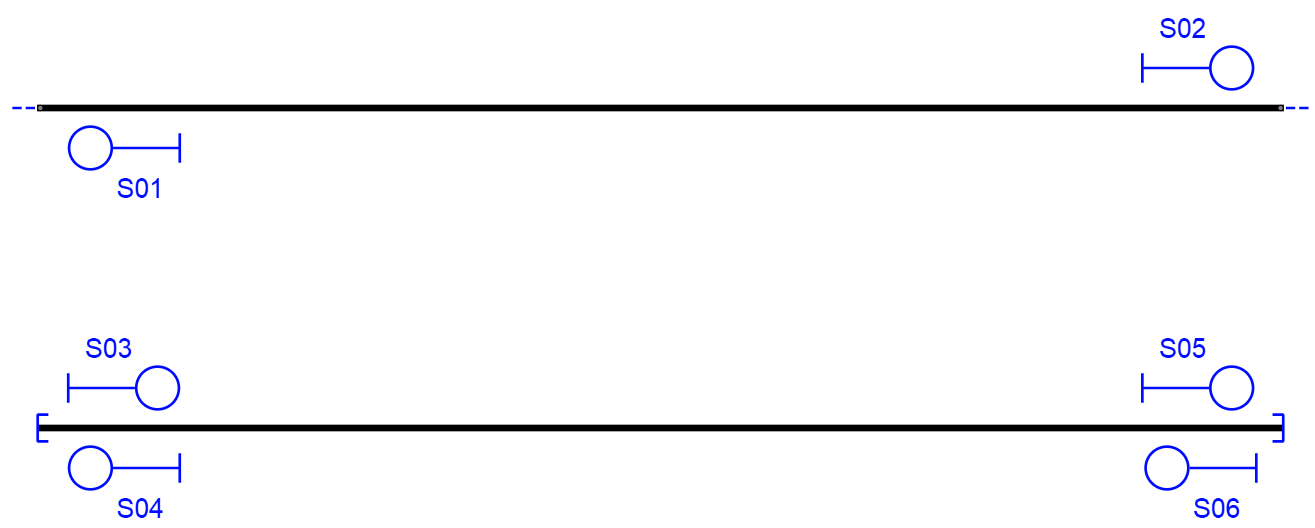
\includegraphics[width=1\textwidth]{Figuras/limites.PNG}
        \centering\caption{Señalamiento generado para finales de vía relativos y absolutos.}
        \label{fig:signal_border}
    \end{figure}
    
    El RNA detecta los \textit{line borders} en la vía superior y aplica el Algoritmo \ref{alg:lineBorder}, generando las señales de partida S01 para las formaciones que se mueven de derecha a izquierda y la señal de partida S02 para las formaciones que se mueven de izquierda a derecha, saliendo de la región mostrada en la Figura \ref{fig:signal_border}. Además, al detectar los \textit{buffer stops} en la vía inferior, el RNA aplica el Algoritmo \ref{alg:bufferStop}, generando cuatro nuevas señales. Las señales S04 y S05 son señales de parada para indicar a las formaciones que deben detenerse antes de colisionar con el final de la vía al transitar de derecha a izquierda o viceversa, respectivamente. Las señales S03 y S06 permiten a las formaciones reanudar su marcha en sentido contrario al que venían circulando, retomando su lugar en la red ferroviaria.
\subsection{Detectores}

\lipsum[1]

\begin{algorithm}[hbt!]
            \caption{Train detection elements algorithm}\label{alg:RJ}
            \DontPrintSemicolon
            %\SetAlgoLined
            \SetNoFillComment
            \LinesNotNumbered 
            \For { netElement WITH AxleCounters or RailJoints }
            {
                Track.Length = Length ( between RailJoints )\;
                \If { Track.Length $>$ FIXED\_LENGTH }
                {
                    [Signals] $\gets$ ADD circulation signal $>>>$\;
                    [Signals] $\gets$ ADD circulation signal $<<<$\;
                }
            }
            \KwResult{[Signals]} 
        \end{algorithm} 
\subsection{Plataformas ferroviarias}

    % Autoridad > derecho limitado a una porcion
    % Claridad > autoridad no ambigua
    % Anticipacion > avisar con antelacion
    % Granularidad > rutas cortas y funcionales
    % Terminalidad > avisar fin de via
    % Infraestructura > avisar de infraestructura
    % No bloqueo > circulacion fluida

    En la Sección \ref{sec:platform} definimos la clase platform que modela a las plataformas ferroviarias. Las plataformas ferroviarias son un punto del recorrido donde las formaciones pueden detenerse, algunas veces de forma opcional dependiendo el itinerario, para que los pasajeros desciendan y nuevos pasajeros puedan ascender. Claramente existe una limitación de autoridad, las formaciones necesitan un nuevo permiso para continuar circulando una vez alcanzada la plataforma. Permiso que será otorgado o negado según el estado del sistema a continuación del recorrido. Las plataformas ferroviarias suelen encontrarse en zonas pobladas, cerca de otras infraestructuras, zonas comerciales o residenciales, por lo que avisar con antelación al maquinista que debe disminuir la marcha y/o detenerse es esencial.

    Además, es posible que las formaciones convivan con otras formaciones que también hacen uso de la estación, por lo que las señales deben ser unívocas y claras. Algunas estaciones pueden contener fines de vías o ramificaciones hacia talleres u otros ramales, por lo que también se aplica el principio de terminalidad ($P_5$) y granuralidad ($P_4$). Finalmente, es importante el mantener una circulación fluida de las formaciones, de modo de no retrasar el itinerario de las formaciones que vienen detrás, por lo que se deberá aplicar el principio de no bloqueo ($P_7$).

    En el Algoritmo \ref{alg:PTF} definimos a la señal de partida como la única señal necesaria para operar una plataforma, asumiendo que la señal de ingreso de la misma será dada por otra instancia previa. De no existir otro elemento cercano por el cual se genere una señal, se puede asumir que la distancia a la plataforma es muy larga y, por lo tanto, se aplicaría el Algoritmo \ref{alg:RJ}, protegiendo a la plataforma. En el caso de que la vía sea bidireccional se añadiran señales de partida para ambos sentidos.

    \begin{algorithm}[hbt!]
        \caption{Algoritmo de generación de señalamiento para platforms.}\label{alg:PTF}
        \DontPrintSemicolon
        %\SetAlgoLined
        \SetNoFillComment
        \LinesNotNumbered 
        \For { netElement WITH Platform }
        {
            \tcc{Before leaving platform from left}
            [Signals] $\gets$ ADD departure signal $\gg\gg$\;
            \tcc{After leaving platform from right}
            [Signals] $\gets$ ADD departure signal $\ll\ll$\;
        }
        \KwResult{[Signals]} 
    \end{algorithm}

    Aplicando el Algoritmo \ref{alg:PTF} a un sistema de dos vías paralelas con plataformas pertenecientes a la misma estación obtenemos el resultado ilustrado en la Figura \ref{fig:signal_platform}.Se asumieron que ambas vías son bidireccionales, en caso contrario solo se generarían las señales S01 y S02.
    
    \begin{figure}[h!]
        \centering
        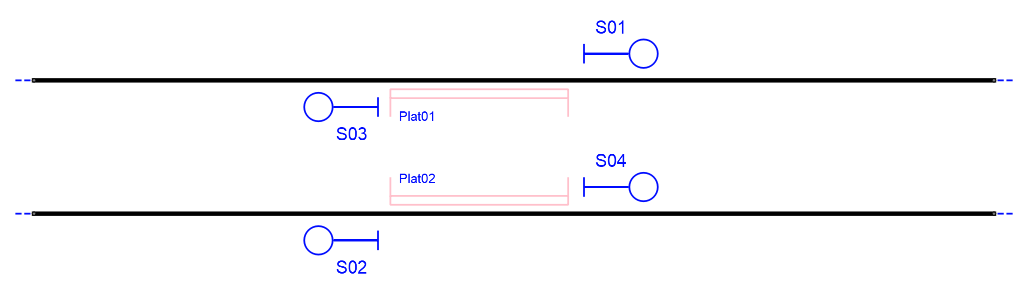
\includegraphics[width=1\textwidth]{Figuras/platforms.PNG}
        \centering\caption{Señalamiento generado para estaciones ferroviarias.}
        \label{fig:signal_platform}
    \end{figure}
    
    Una formación que circule de izquierda a derecha deberá detenerse antes de la señal S01, en caso de utilizar la vía superior, o antes de la señal S04, en caso de utilizar la vía inferior. Análogamente, las formaciones deberán detenerse antes de las señales S03 y S02 en el caso de transitar de derecha a izquierda por la vía superior o inferior respectivamente. Sólo cuando estas señales otorguen a la formación autoridad para circular podrán reanudar su marcha hasta la próxima señal disponible, fuera del alcance de lo ilustrado en la Figura \ref{fig:signal_platform}.
\subsection{Cruces de via}

\lipsum[1-2]

    \begin{algorithm}[hbt!]
        \caption{Level crossing algorithm}\label{alg:LC}
        \DontPrintSemicolon
        %\SetAlgoLined
        \SetNoFillComment
        \LinesNotNumbered 
        \For { netElement WITH LevelCrossing }
        {
            \tcc{Before reaching level crossing}
            [Signals] $\gets$ ADD circulation signal $>>>$\;
            \tcc{After leaving level crossing}
            [Signals] $\gets$ ADD circulation signal $<<<$\;
        }
        \KwResult{[Signals]} 
    \end{algorithm}

\lipsum[1]
\includegraphics{example-image}\\
\lipsum[1-2]
\subsection{Maquinas de cambios}
	\label{sec:signal_switches}
	
    % Autoridad > derecho limitado a una porcion
    % Claridad > autoridad no ambigua
    % Anticipacion > avisar con antelacion
    % Granularidad > rutas cortas y funcionales
    % Terminalidad > avisar fin de via
    % Infraestructura > avisar de infraestructura
    % No bloqueo > circulacion fluida
    
    En la Sección \ref{sec:switches} definimos la clase switches que modela a las máquinas de cambios. Las máquinas de cambios son de los elementos ferroviarios mas críticos de la red. Por lo tanto, se deberá aplicar al principio de infraestructura a cada una de sus entradas. Además, las máquinas de cambios actúan como una frontera entre las ramas principales de la red, donde se circula a mayor velocidad, y las ramas secundarias, donde se circula a una velocidad menor. Esto divide las rutas en dos o mas rutas, aplicando el principio de autoridad y granularidad. Finalmente, por el principio de no bloqueo, será necesario generar señales de diferente tipo para las ramas principales y las secundarias, priorizando las primeras. Esto puede cumplirse si otorgamos señales de circulación de tres o mas aspectos a la rama principal y señales de maniobra para utilizar una rama secundaria como salida o entrada de la red.
    
    En el Algoritmo \ref{alg:SW} definimos al punto de acceso de inicio como la vía desde la cual la trayectoria de la formación se bifurca, para lo cual se genera una señal de circulación para continuar por la rama principal y una señal de maniobra para acceder a la rama secundaria. Además, se añade una señal de circulación en la rama principal y una señal de maniobra en la rama secundaria, ambas en sentido contrario, para poder retornar al punto de inicio. 
    
    \begin{algorithm}[hbt!]
        \caption{Algoritmo de generación de señalamiento para Switches}\label{alg:SW}
        \DontPrintSemicolon
        %\SetAlgoLined
        \SetNoFillComment
        \LinesNotNumbered 
        \For { Switch in Switches }
        {
            \tcc{All signals must point to switch}
            \Switch{ Switch.Type }
            {
                \Case{Start}
                {
                    [Signals] $\gets$ ADD circulation signal\;
                    [Signals] $\gets$ ADD maneuver signal\;
                }
                \Case{Continue branch}
                {
                    [Signals] $\gets$ ADD circulation signal\;
                }
                \Case{Detour branch}
                {
                    [Signals] $\gets$ ADD maneuver signal\;
                }
            }   
        }
        \KwResult{[Signals]} 
    \end{algorithm}

    Aplicando el Algoritmo \ref{alg:SW} a un sistema de vías que se bifurcan obtenemos el resultado ilustrado en la Figura \ref{fig:signal_swithces}. Se asumieron que ambas vías son bidireccionales. En caso contrario, si el sentido de circulación es únicamente de bifurcación, las señales de retorno S02 y S03 no son necesarias. Si el sentido de circulación fuese de derecha a izquierda, las señales de inicio S01 no son necesarias.
    
    \begin{figure}[h!]
        \centering
        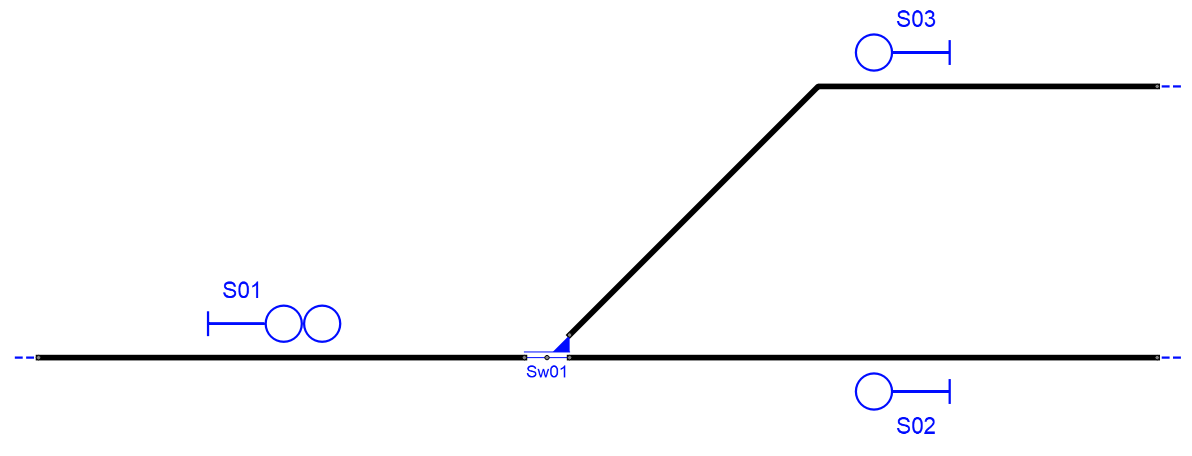
\includegraphics[width=1\textwidth]{Figuras/switches.PNG}
        \centering\caption{Señalamiento generado para cambios de vías.}
        \label{fig:signal_swithces}
    \end{figure}
    
    Una formación que circule de izquierda a derecha deberá detenerse antes de la señal S01. El aspecto mas cercano al poste de la señal S01 indicará si la formación puede circular por la vía principal, como se explicó en la Sección \ref{sec:signals}, previa confirmación por parte del sistema de enclavamiento de que el cambio Sw01 se encuentra en posición normal. De la misma forma, el sistema de enclavamiento confirmará que el cambio Sw01 se encuentra en posición reverso previo a habilitar la circulación por la vía secundaria mediante el aspecto mas alejado al poste de la señal S01.

    Una formación circulando de derecha a izquierda hará uso de las señales S02 y S03 si se encuentran en las vías principal o secundaria respectivamente. Las señales se habilitarán si el sistema de enclavamientos confirma que el cambio Sw01 se encuentra en la posición normal o reverso respectivamente y si no hay formaciones ocupando la vía de inicio donde se encuentra la señal S01, continuando su marcha hasta la próxima señal disponible, fuera del alcance de lo ilustrado en la Figura \ref{fig:signal_swithces}.    
\section{Algoritmos de simplificación de señalamiento}
    \label{sec:simplificacion}

    % Autoridad > derecho limitado a una porcion
    % Claridad > autoridad no ambigua
    % Anticipacion > avisar con antelacion
    % Granularidad > rutas cortas y funcionales
    % Terminalidad > avisar fin de via
    % Infraestructura > avisar de infraestructura
    % No bloqueo > circulacion fluida
    
    Una vez finalizada la generación de señalamiento para cada elemento ferroviario, es necesario abordar el segundo miembro de la Fórmula \ref{frm:signal_1} explicada al comienzo de la Sección \ref{sec:generacion}. El señalamiento total para un sistema de N elementos ferroviarios será la suma de las señales necesarias para proteger a esos N elementos ferroviarios. Es inevitable que algunas señales se solapen con otras espacial o funcionalmente. Incluso algunas señales podrían contradecir a otras, oponiéndose al principio de claridad. La abundancia de señales puede hacer las rutas tan cortas que la autoridad estaría limitada a pequeñas porciones de la red, haciendo inviable una circulación fluida sobre la red.

    La simplificación del señalamiento se sustenta en dos algoritmos básicos: simplificación por herencia vertical y simplificación por herencia horizontal. Los dos algoritmos pueden aplicarse en cualquier orden, aunque los algoritmos de herencia vertical solamente se pueden aplicar en redes ramificadas que tengan máquinas de cambios. 

    El proceso de simplificación finaliza con el algoritmo de limpieza, que elimina todas las señales redundantes en base a un nivel de prioridades. Estas prioridades se relacionan directamente con qué elemento ferroviario el RNA intentaba proteger con esta señal, reteniendo la señal mas importante y eliminando el resto. También se combinan señales muy próximas en una vecindad y se borran señales contradictorias o redundantes, para obtener el señalamiento definitivo.    

 	\subsection{Algoritmo de simplificación por herencia vertical}
	\label{sec:vertical}
	% Autoridad > derecho limitado a una porcion
	% Claridad > autoridad no ambigua
	% Anticipacion > avisar con antelacion
	% Granularidad > rutas cortas y funcionales
	% Terminalidad > avisar fin de via
	% Infraestructura > avisar de infraestructura
	% No bloqueo > circulacion fluida
	
	Como se explicó en la Sección \ref{sec:switches}, una máquina de cambios bifurca la vía principal en dos: una vía que continúa la rama principal y otra vía que se convierte en una rama secundaria. Tanto la vía de continuación como la vía ramificada pueden tener otra máquina de cambios que, a su vez, vuelve a dividir el trazado ferroviario en dos. Esto incrementa más y más el nivel de complejidad de la red, añadiendo caminos divergentes al principal que luego, mas adelante, podrían, o no, volver a converger utilizando mas máquinas de cambios. Cada divergencia aporta un nivel de profundidad a la red, mientras que cada convergencia reduce en uno el nivel de profundidad.
	
	Una máquina de cambios que tiene en cualquiera de sus ramas divergentes el nodo de inicio de otra máquina de cambios a una distancia pequeña es un cambio compuesto. Los cambios compuestos requieren considerar a ambas máquinas de cambios como una sola, ya que es necesario posicionar ambos mecanismos para completar un movimiento. El ejemplo de La Figura \ref{fig:signal_vertical_1} ayudará a clarificar el concepto de cambios compuestos e introducir el Algoritmo de simplificación por herencia vertical.	

	\begin{figure}[H]
		\centering
		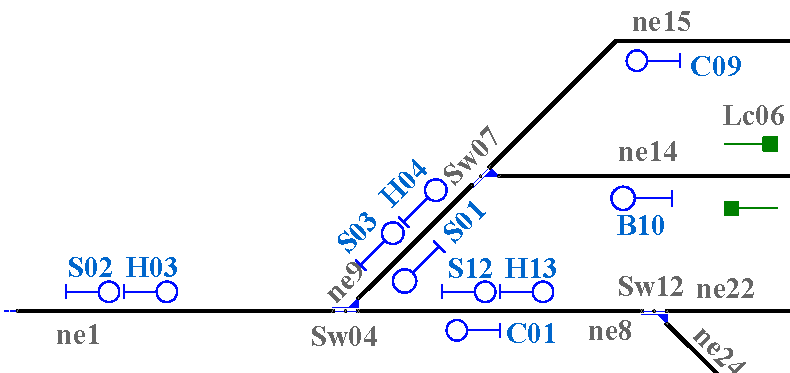
\includegraphics[width=1\textwidth]{Figuras/Figure8_Crop.pdf}
		\centering\caption{Señalamiento generado, simplificado por algoritmo de herencia vertical.}
		\label{fig:signal_vertical_1}
	\end{figure}
	
	En la Sección \ref{sec:signal_switches} se introdujo el Algoritmo \ref{alg:SW} que define la asignación de señalamiento para los cambios de vías: una señal de circulación (S) y de maniobra (H) para el nodo de inicio (S), una señal de circulación para el nodo de continuación (C) y una señal de maniobras para el nodo de desvío (B). El Algoritmo \ref{alg:SW} se aplicó de forma independiente a las máquinas de cambios Sw04, Sw07 y Sw12 y se obtuvo el señalamiento de la Figura \ref{fig:signal_vertical_1}. No obstante, el señalamiento generado no cumple con el principio de no bloqueo, al situar las señales S03, H04, B01, S12, H13 y C01 en las secciones correspondientes a los netElements ne9 y ne8. De esa manera, las formaciones podrían detenerse en esas secciones si las mencionadas señales presentasen un aspecto rojo.
	
	Una formación detenida en la sección correspondiente al \textit{netElement} ne9 no permitiría mover el cambio de vía Sw04, al tener parte de la formación aún en ne1. Tampoco permitiría accionar el cambio de vías Sw07 al no haber finalizado el movimiento. Análogamente, loa mismo ocurriría para una formación detenida en la sección correspondiente al \textit{netElement} ne8. Es necesario que el movimiento finalice, despejando las secciones y permitiendo que otras formaciones utilicen los cambios de vías Sw04 y Sw07, o cualquier combinación de mas de un cambio de vías.
	
	Para solucionar el problema expuesto, el RNA aplica el Algoritmo \ref{alg:vertical} de simplificación por herencia vertical para reposicionar las señales situadas en zonas conflictivas. A diferencia del señalamiento explicado en la Sección \ref{sec:generacion}, las señales que protegen a un cambio de vías B situado en una rama mas profunda de la red no se encuentran inmediatamente precediendo al cambio de vías B. Estas señales son movidas a ramas de menor profundidad con suficiente espacio físico para contenerlas, situándose precediendo a otro cambio de vías A que decimos que ha \emph{heredado} el señalamiento del cambio de vía B.
		
	\begin{algorithm}[H]
        \caption{Algoritmo de simplificación por herencia vertical}\label{alg:vertical}
        \DontPrintSemicolon
        %\SetAlgoLined
        \SetNoFillComment
        \LinesNotNumbered 
        \For{ each Signal protecting a Sw\_A }
        {
            \For{each Sw\_B != Sw\_A}
            {
                \tcc{Criteria \#0}
                \If{distance(Sw\_A,Sw\_B) $>$ MIN\_DISTANCE}
                {
                    Continue\;
                }
                \If{S in Sw\_A.Branch also in Sw\_B.Start} 
                {
                   \tcc{Criteria \#1}
                   \If{S points to Sw\_B.Start}
                   {
                        Move S to Sw\_A.Start\;
                   }
                   \tcc{Criteria \#2}
                   \If{S points to Sw\_A.Branch}
                   {
                        Move S to Sw\_B.Continue\;
                        Move S to Sw\_B.Branch\;
                   }
                }
                \If{S in Sw\_A.Continue also in Sw\_B.Start}
                {
                   \tcc{Criteria \#3}
                   \If{S points to Sw\_B.Start}
                   {
                        Move S to Sw\_A.Start\;
                   }
                   \tcc{Criteria \#4}
                   \If{S points to Sw\_A.Continue}
                   {
                        Move S to Sw\_B.Continue\;
                        Move S to Sw\_B.Branch\;
                   }
                }
            }
        
        }
        \KwResult{[Signals]} 
    \end{algorithm}

    Como puede apreciarse en el Algoritmo \ref{alg:vertical}, existen cinco criterios a considerar para aplicar la herencia vertical. El primer criterio es excluyente, si la distancia entre ambas máquinas de cambios supera un parámetro determinado entonces el algoritmo no se aplica, al existir suficiente distancia para situar el señalamiento sin generar obstrucciones debido a formaciones detenidas entre ambos. Cuando la distancia entre las máquinas de cambios es menor a lo esperado, se aplican los otros cuatro criterios, en función de que nodos conectan entre sí la vía que comparten.
    
    Definiendo al cambio de vías A como el cambio principal y el cambio de vías B como el cambio secundario situado en alguna de las ramificaciones del cambio de vías A, podemos diferenciar dos casos: que el señalamiento se encuentre en la rama de continuación del cambio de vías A o se encuentre en la rama de desvío. Además, este señalamiento puede estar apuntando al cambio de vías A o al cambio de vías B, protegiéndolo respectivamente. 
    
    El criterio para el desplazamiento del señalamiento busca cumplir el principio de Anticipación, el principio de Infraestructura y el principio de no bloqueo. Para eso, las señales son adelantadas, desplazándolas en sentido opuesto al que apuntan. Si el señalamiento se encuentra en la rama de desvío o continuación del cambio de vías A es indistinto, lo importante es a donde apuntan las señales. Si estas apuntan hacia el nodo de inicio del cambio de vías B, deben ser desplazadas, sin alterar su cantidad, hacia el nodo de inicio del cambio de vías A. 
    
    En el caso particular de que las señales en la zona conflictiva apunten hacia el cambio de vías A, tanto a su nodo de desvío como al nodo de continuidad, las mismas deberían moverse en sentido contrario al que apuntan. Sin embargo, en esa dirección la red se ramifica en dos debido al cambio de vías B. En este caso, las señales mueven duplicadas, a la rama de continuación y a la rama de desvío del cambio de vías B, en su totalidad.
    
    Aplicando el Algoritmo \ref{alg:vertical} de herencia vertical al ejemplo de la Figura \ref{fig:signal_vertical_1} obtenemos el señalamiento de la Figura \ref{fig:signal_vertical_2}. Las señales S03, H04, B01, S12, S13 y C01 serán adelantadas para despejar las secciones correspondientes a los netElements ne9 y ne8. Debido a esto, los tres cambios de vías se usarán de forma complementaria, creando los siguientes cambios compuestos: $Sw_{04}^R+Sw_{07}^N$, $Sw_{04}^R+Sw_{07}^R$, $Sw_{04}^N+Sw_{12}^N$ y $Sw_{04}^N+Sw_{12}^R$. Los cuales se leen, considerando el ejemplo del cambio compuesto $Sw_{04}^R+Sw_{07}^N$, de la siguiente manera: el cambio de vías Sw04 en posición normal y el cambio de vías Sw07 en posición reversa.
    
    \begin{figure}[H]
    	\centering
    	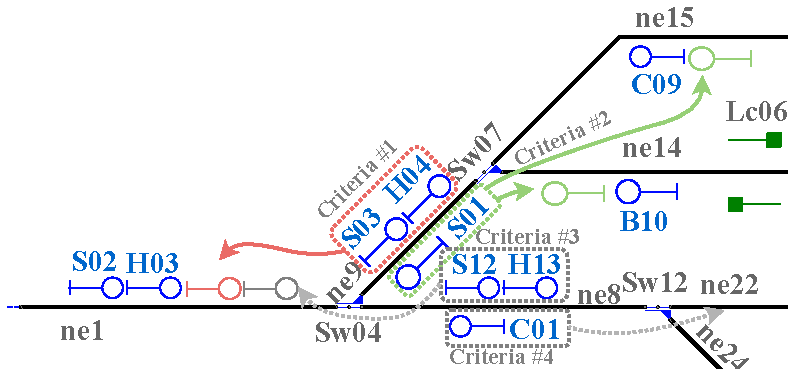
\includegraphics[width=1\textwidth]{Figuras/Figure9_Crop.pdf}
    	\centering\caption{Señalamiento generado, simplificado por algoritmo de herencia vertical.}
    	\label{fig:signal_vertical_2}
    \end{figure}
    
    En el caso de las señales S03 y H04 que apuntan al nodo de inicio del cambio de vías Sw07, son desplazadas en sentido contrario al que apuntan, aplicando el criterio \#1. Estas señales son movidas hasta el nodo de continuación del cambio de vías Sw04, correspondiente al netElement ne1, protegiendo el inicio del cambio compuesto $Sw_{04}^R+Sw_{07}^N$ y $Sw_{04}^R+Sw_{07}^R$ . A estas señales se le suman las señales S12 y H13 situadas en la sección correspondiente al netElement ne8 que, aplicando el criterio \#3, son desplazadas al nodo de inicio del cambio de vías Sw04, protegiendo el inicio del cambio compuesto $Sw_{04}^N+Sw_{12}^N$ y $Sw_{04}^N+Sw_{12}^R$.
    
    La señal B01 apunta al nodo de desvío del cambio de vías Sw04 y, por el criterio \#2, debe ser duplicada y movida. Una señal se posiciona en la sección correspondiente al netElement ne15 y la otra a la sección asociada al netElement ne14. De esta manera, la señal S01a y S01b seguirán protegiendo el nodo de desvío del cambio de vías Sw04, pero previamente tendrán que hacer uso del cambio de vías Sw07 en cualquiera de sus dos posiciones, protegiendo los nodos de cambio y continuación del cambio compuesto $Sw_{04}^R+Sw_{07}^N$ y $Sw_{04}^R+Sw_{07}^R$. De igual manera, la señal C01 es movida y duplicada a las secciones correspondientes a los netElements ne22 y ne24, debido al criterio \#4. Estas nuevas señales C01a y C01b continúan protegiendo el nodo de continuación del cambio de vías Sw04, pero ahora deberán, adicionalmente, hacer uso del cambio de vías Sw12, protegiendo los nodos de continuación y desvío del cambio compuesto $Sw_{04}^N+Sw_{12}^N$ y $Sw_{04}^N+Sw_{12}^R$.
    
    El Algoritmo \ref{alg:vertical} de herencia vertical es exitoso a la hora de despejar las zonas críticas entre cambios de vías muy cercanos. No obstante, también incrementa la cantidad de señales, como en el caso de las señales S01 y C01 al ser desplazadas en sentido divergente por los cambios de vías Sw07 y Sw12. Además, el Algoritmo \ref{alg:vertical} de herencia vertical no es aplicable solo a una dupla de cambios de vías, sino que puede ser aplicado para cualquier conjunto de cambios de vías. Esto provoca que las señales se hereden de forma iterativa hasta encontrar un cambio de vías con suficiente espacio para albergar las señales. Debido a esto, la cantidad de señales al comienzo de un cambio de vías previo a una ramificación profunda de la red tendrá una gran cantidad de señales.
    
    En el caso del ejemplo de las Figuras \ref{fig:signal_vertical_1} y \ref{fig:signal_vertical_2}, el algoritmo concluye con seis señales en el nodo de inicio de los cuatro cambios compuestos. Estas seis señales deberán habilitar cuatro caminos a transitar desde ne1: hacia ne15, hacia ne14, hacia ne22 y hacia ne24. Es claro que, teniendo mas señales que caminos a habilitar, será necesario un algoritmo de limpieza de señales duplicadas y/o que ya no tengan una utilidad en el señalamiento. El proceso de simplificación es explicado en profundidad en la Sección \ref{sec:limpieza}.
    \subsection{Algoritmo de herencia horizontal}

\lipsum[1]

\begin{algorithm}[hbt!]
        \caption{Horizontal inheritance algorithm}\label{alg:horizontal}
        \DontPrintSemicolon
        %\SetAlgoLined
        \SetNoFillComment
        \LinesNotNumbered 
        \For{ each netElement }
        {
            \For{ each object in netElement }
            {
                \If{dist(Obj\_A,Obj\_B) $<$ MIN\_DISTANCE }
                {
                    move\_signals\_between(Obj\_A,Obj\_B)
                }
            }
        }
        \KwResult{[Signals]} 
    \end{algorithm}

    \lipsum[1-3]
    \subsection{Limpieza de señales}
	\label{sec:limpieza}

	% Autoridad > derecho limitado a una porcion
	% Claridad > autoridad no ambigua
	% Anticipacion > avisar con antelacion
	% Granularidad > rutas cortas y funcionales
	% Terminalidad > avisar fin de via
	% Infraestructura > avisar de infraestructura
	% No bloqueo > circulacion fluida
	
	El Algoritmo \ref{alg:vertical} de simplificación por herencia vertical y el Algoritmo \ref{alg:horizontal} de simplificación por herencia horizontal tienen diferentes efectos en la cantidad de señales totales. El Algoritmo de herencia horizontal mueve las señales entre elementos cuando no existe suficiente espacio entre ellos. Sin embargo, el Algoritmo de herencia vertical duplica la cantidad de señales si se aplica el criterio \#2 o el \#4. Todos los algoritmos que utiliza el RNA pueden aplicarse de forma iterativa si las condiciones lo permiten, pero particularmente el Algoritmo \ref{alg:vertical} duplicará las señales por cada nivel de profundidad de la red ferroviaria. Esto llevará a tener mas señales que las necesarias en algunos netElements. Este exceso de señales deben eliminarse para mantener una proporción uno a uno entre una señal y una funcionalidad específica. El Algoritmo \ref{alg:reduction} se ocupa de la limpieza de las señales que se encuentran muy próximas entre si, eliminando siempre las que tengan menor prioridad. 

	\begin{algorithm}[H]
        \caption{Signal reduction algorithm}\label{alg:reduction}
        \DontPrintSemicolon
        %\SetAlgoLined
        \SetNoFillComment
        \LinesNotNumbered 
        Sources = $\{$ T,L,S,B,P,C,J,X $\}$\;
        \For{ Sig\_A \& Sig\_B in [Signals]}
        {
            \If{ A != B  \& Sig\_A.From == Sig\_B.From }
            {
             Signalling\_zones.Pos = detect\_next\_dangers ( Sig\_A )\;
             A.Pos,B.Pos = Sig\_A.Pos,Sig\_B\;
             Safe = zone\_between(Signalling\_zones.Pos,A.Pos,B.Pos)\;
                 \If{ NOT safe }
                 {
                    \If{ $|A.Pos,B.Pos|$ $<$ MIN\_DISTANCE }
                    {
                        \If{ Sig\_A \& Sig\_B same orientation }
                        {
                            \If{ Sig\_A \& Sig\_B same direction }
                            {
                                \If { Sig\_A \& Sig\_B type "Circ" }
                                {
                                    \If{ Sig\_A.Idx $<$ Sig\_B.Idx }
                                    {
                                        delete Sig\_B  else Sig\_A
                                    }
                                    %{
                                    %    delete( Sig\_A )
                                    %}
                                }
                            }
                        }
                        \If{ Sig\_A \& Sig\_B different source}
                        {
                            delete\_lowest\_priority( Sig\_A,Sig\_B )\;
                        }
                    }
                }
            }
        }
        \KwResult{[Signals]} 
    \end{algorithm}

	La prioridad es definida según el origen de cada señal. Como se explicó en la Sección \ref{sec:generacion}, las señales pueden tener diferentes etiquetas en función de que elemento ferroviario están protegiendo. Las señales S C B y H protegen los cambios de vías, las señales P a las plataformas, las señales J a las junturas, las señales X a los cruces de vías. Todas ellas son señales de circulación, salvo las señales B y H que son de maniobras. La prioridad mas alta fue asignada a las señales que protegen los finales de vía absolutos (T) y relativos (L) porque son las únicas señales de parada que no pueden ser reemplazadas por señales menos restrictivas. 
	
	Esto no significa que todas las señales que protegen los finales de vía (T) eliminarán todas las señales de los pasos a nivel (X), sino que de tener otra señal cercana del mismo tipo que apunte en la misma dirección y sentido, pero de mayor prioridad, será ésta quien cumpla la función de proteger al paso a nivel. Las señales pueden tener diferentes roles, como ser señales de parada, de circulación, de partida o maniobra. Las señales de parada son absolutas y se utilizan en finales de vía, mientras que las señales de partida se utilizan para reiniciar la marcha de la formación. Las primeras poseen un aspecto rojo, mientras que las segundas pueden tener hasta tres aspectos. Las señales de circulación poseen tres aspectos y permiten velocidades mas altas en las ramas principales de la red. Las señales de maniobra poseen solamente dos aspectos y son utilizadas en los desvíos, tanto en ramas divergentes como en convergentes.
	
	En el caso de que dos señales que tengan igual dirección, sentido y origen, pero no tengan una región de señalamiento entre ellas, deban ser simplificadas. En este caso, se decidió eliminar la señal con índice mas alto. Esto se debe a que, una vez generado el señalamiento para cada elemento, las señales de mayor índice serán las producidas por los Algoritmos de herencia horizontal y vertical, que tiendan a añadir señales que con mucha probabilidad deben ser eliminadas a posteriori.
	
    Es importante resaltar que la asignación de prioridades es de vital importancia para la seguridad. Por ejemplo, que las señales B tengan mayor prioridad que las señales P. Si la plataforma se encuentra lo suficientemente alejada de un cambio de vías, una señal de maniobra que protege el cambio de vías no puede reemplazar una señal de circulación que protege a una plataforma porque siempre habrá una plataforma entre ambos y, por lo tanto, una región de señalamiento. Sin embargo, si la plataforma se encuentra lo suficientemente cerca del cambio de vías, la señal de maniobras B se movería hacia la región de señalamiento donde se encuentra la señal de circulación P, debido al Algoritmo \ref{alg:horizontal} de herencia horizontal por el cual dos elementos ferroviarios muy próximos combinan sus regiones de señalamiento. Por lo tanto, la señal B de dos aspectos reemplazara a la señal P de tres aspectos, reduciendo la velocidad máxima permitida en esa zona de la red ferroviaria, incrementando la seguridad de la red.	
\section{Generacion de tablas de enclavamiento}

\lipsum[1]

\begin{algorithm}[hbt!]
        \caption{Route detection algorithm}\label{alg:routes}
        \DontPrintSemicolon
        %\SetAlgoLined
        \SetNoFillComment
        \LinesNotNumbered 
        Routes = [], route = 0\;
        \For{ start in [Signals] }
        {
            \tcc{Find manoeuvre and circulation signals}
            \If{ start != "Stop" }
            {
                dir = start\_sig.Direction\;
                \tcc{Find next signal w/ same direction}
                
                end = find\_next\_signal(start,[Signals])\;

                [paths] = find(start.node,end.node,graph)\;
                
                \For{ node in [paths] }
                {
                    \tcc{Find rail objects within path}
                    sws = find(graph[node],switches)\;
                    lc = find(graph[node],levelCrossings)\;
                    ptf = find(graph[node],platforms)\;
                    %route ++\;
                    Routes[route++] = $\{$start,end,dir,node,sws,lc,ptf$\}$\;
                }
            }
        }
        \KwResult{[Routes]} 
    \end{algorithm}
\section{Validacion de tablas de enclavamiento}

\lipsum[1]
\section{Validación de principios de señalamiento ferroviario}
	\label{sec:validar_principios}
	
	% Autoridad > todas las rutas combinadas cubren toda la traza ferroviaria.
	% Claridad > autoridad no ambigua.
	% Anticipacion > avisar con antelacion.
	% Granularidad > rutas cortas y funcionales.
	% Terminalidad > avisar fin de via.
	% Infraestructura > avisar de infraestructura.
	% No bloqueo > circulacion fluida.
				
	En esta sección se abordará el proceso de validación de cada uno de los principios ferroviarios establecidos en la Sección \ref{sec:principios}, como parte del proceso expuesto en la Sección \ref{sec:validacion}. Para ello, serán abordados de manera genérica cada uno de los principios de señalamiento junto con el algoritmo que el RNA utiliza para validarlo, previo a exportar el señalamiento generado.
	
	\subsection{Validación del principio de autoridad}
		% Autoridad > todas las rutas combinadas cubren toda la traza ferroviaria.
		
		El principio de autoridad radica en que las rutas otorgan a las formaciones un permiso de uso limitado para circular por las vías. No obstante, la combinación de todas las autoridades disponibles de ser otorgadas deben cubrir la totalidad de la traza ferroviaria. Es decir, no debe existir ninguna sección de vía que se encuentre fuera del alcance de las rutas y, por lo tanto, aislada de la red. Puede darse el caso de que una sección de vía tenga una ruta de entrada o de salida, pero no ambas. También puede darse el caso de que la sección de vía sea transitada, pero no sea ni inicio ni final de ninguna ruta.
		
		El RNA utiliza el Algoritmo \ref{alg:ppio_autoridad} para validar el principio de autoridad comparando los netElements alcanzados por las rutas disponibles, con la lista de netElements potenciales de ser alcanzados. Esta última salvedad deja fuera las secciones de vías que preceden a una señal de circulación posterior a un final de vía relativo (lineBuffer). Esto se realiza ya que estas secciones de vía son transitadas por rutas fuera de la locación bajo análisis, rutas que terminan en la señal de circulación mencionada.

		\begin{algorithm}[hbt!]
			\caption{Algoritmo de validación del principio de autoridad.}\label{alg:ppio_autoridad}
			\DontPrintSemicolon
			%\SetAlgoLined
			\SetNoFillComment
			\LinesNotNumbered 
			Validated = False\;
			$\{$Routes$\}$, $\{$netElements$\}$ without netElements with lineBuffer\; 
			\tcc{Validate that every route covers all the railway tracks.}
			\For{route in $\{$Routes$\}$}
			{
				\If{route[begin] in $\{$netElements$\}$}
				{
					Remove route[begin] from $\{$netElements$\}$\; 
				}
				\If{route[end] in $\{$netElements$\}$}
				{
					Remove route[end] from $\{$netElements$\}$\; 
				}
				\For{track in route[paths]}
				{
					\If{track in $\{$netElements$\}$}
					{
						Remove track from $\{$netElements$\}$\; 
					} 
				}
			}
			\If{$\{$netElements$\}$ is Empty}
			{
				Validated = True\; 
			} 
			\KwResult{Validated} 
		\end{algorithm}
		
		Se asume inicialmente que la validación es fallida por defecto. Si al finalizar el Algoritmo \ref{alg:ppio_autoridad} no existe ningún netElement remanente en la lista, se considera que la validación es exitosa.	
			
	\subsection{Validación del principio de claridad}
		% Claridad > autoridad no ambigua
		
		El principio de claridad radica en que el señalamiento no posee señales ambiguas. Es decir, no existen dos rutas distintas que otorguen autoridad sobre las mismas secciones de vía, en el mismo sentido, utilizando la misma infraestructura. En otras palabras, las rutas en una misma dirección y sentido no se solapan, cada una comienza donde otra ha terminado.
		
		El RNA utiliza el Algoritmo \ref{alg:ppio_claridad} para validar el principio de claridad, generando una red de grafos dirigidos. La misma se constituye utilizando todas las rutas definidas por el RNA como aristas, y a los netElements que conectan como nodos de la red. Si se detecta que existen dos rutas R$^{\prime}$ y R$^{\prime\prime}$ que conectan dos nodos A y B en el mismo sentido, utilizando la misma infraestructura, entonces se dice que las rutas son ambiguas y el principio de claridad no se cumple.
		
		\begin{algorithm}[hbt!]
			\caption{Algoritmo de validación del principio de claridad.}\label{alg:ppio_claridad}
			\DontPrintSemicolon
			%\SetAlgoLined
			\SetNoFillComment
			\LinesNotNumbered 
			Validated = False\;
			$\{$Routes$\}$\; 
			\tcc{Validate that every netElement is reached by one route only.}
			\For{route in $\{$Routes$\}$}
			{
				begin = route[begin]\;
				end = route[end]\;
				index = route[index] \;
				direction = route[direction]\;
				digraph = create\_digraph(begin,end,index,direction)\;	
			}
			\If{digraph has no redundant routes}
			{
				Validated = True\;
			}
			\KwResult{Validated} 
		\end{algorithm}
		
		Aunque el orden de validación de los principios de señalamiento es indistinto, la confirmación de que las señales son suficientes para alcanzar toda la red (Principio de autoridad) y de que no existen señales ambiguas (Principio de claridad) facilita las siguientes validaciones. Esto se debe a que, con estas dos comprobaciones, ya sabemos que contamos con la mínima cantidad de señales para recorrer la red de forma unívoca, garantizando la correcta logística de la red. Los siguientes principios son necesarios para validar la seguridad del señalamiento generado por el RNA.
		
	\subsection{Validación del principio de anticipación}
		% Anticipacion > avisar con antelacion
		
		El principio de anticipación radica en que existe una señal previo a cada peligro, situada en la zona de señalamiento. Una zona señalamiento puede estar próxima a una curva, al final de la traza ferroviaria o en las inmediaciones de un paso a nivel, una estación, un cambio de vías o cualquier infraestructura ferroviaria a ser protegida. En otras palabras, el señalamiento debe estar distribuido de tal manera que entre dos señales que constituyen una ruta exista un único peligro o situación que quiera la atención del conductor.
		
		El RNA utiliza el Algoritmo \ref{alg:ppio_anticipacion} para validar el principio de anticipación, detectando las regiones de señalamiento como zonas peligro peligrosas, producto del trazado ferroviario (curvas, finales de vía) o de la infraestructura ferroviaria (plataformas, pasos a nivel, etc.). 
		
		\begin{algorithm}[hbt!]
			\caption{Algoritmo de validación del principio de anticipación.}\label{alg:ppio_anticipacion}
			\DontPrintSemicolon
			%\SetAlgoLined
			\SetNoFillComment
			\LinesNotNumbered 
			Validated = True, $\{$Dangers$\}$ = None\;
			$\{$Routes$\}$, $\{$Track$\}$\; 
		
			\tcc{Validate that each danger is protected by the signalling.}
			
			\For{curve in $\{$Tracks$\}$}
			{
				$\{$Dangers$\}$ $\Leftarrow$ ADD curve
			}
			
			\For{element in $\{$Infraestructure$\}$}
			{
				$\{$Dangers$\}$ $\Leftarrow$ ADD element
			}
			
			\For{danger in $\{$Dangers$\}$}
			{
				
				\For{track going into danger}
				{
					\If{track has signal AND signal points to danger}
					{
						Continue\;
					}
					\Else
					{
						Validated = False\; 
						Stop iterations\;
					}
				}	
			}
			
			\KwResult{Validated} 
		\end{algorithm}
		
		A continuación, el Algoritmo \ref{alg:ppio_anticipacion} comprueba que existe una señal para cada dirección del peligro, apuntando en el sentido del mismo. Garantizando de esta forma, que previo a cada peligro inicie o finalice una ruta, en caso de que la ruta sea segura de ser transitada o no, respectivamente.
		
		Una sola región de señalamiento que tenga una de sus entradas sin proteger por una señal es suficiente para que el Algoritmo \ref{alg:ppio_anticipacion} devuelva un resultado negativo. Si todas las entradas de cada región de señalamiento están protegidas por una señal, entonces el principio de anticipación se encuentra cumplido. En el caso de que los elementos ferroviarios se encuentren muy próximos, por herencia horizontal, se consideran un único elemento y sus regiones de señalamiento se simplifican como se explicó en la Sección \ref{sec:horizontal}.
		
	\subsection{Validación del principio de granularidad}
		% Granularidad > rutas cortas y funcionales
		
		El principio de granularidad radica en que las rutas deben ser lo suficientemente cortas como para permitir una logística flexible, pero no tan cortas como para no tener ninguna funcionalidad real. Consideramos, por lo tanto, que el señalamiento debe estar distribuido de tal forma que las rutas tengan una funcionalidad básica. Entre éstas funciones tenemos el uso de un elemento ferroviario específico (o conjunto de elementos ferroviarios, si están muy próximos) o la subdivisión de rutas cuyos tramos originales eran demasiado extensos.
		
		El RNA utiliza el Algoritmo \ref{alg:ppio_granularidad} para validar el principio de granularidad, analizando que elementos ferroviarios se encuentran contenidos en cada ruta y la distancia entre las señales que conforman la misma. Se recorre el listado de rutas generadas por el RNA, que ya establece los elementos contenidos en las rutas, las señales que las definen y la posición de las mismas. En cada ruta se analiza si existen elementos ferroviarios que justifiquen la existencia de la ruta y si el largo de la misma se encuentra entre un rango mínimo y máximo estipulado. Si alguna de estas condiciones se cumple, entonces se procede a analizar la siguiente ruta. En caso contrario, el Algoritmo \ref{alg:ppio_granularidad} finaliza de forma negativa. Si todas las rutas analizadas superan el proceso, entonces el principio de granularidad ha sido validado exitosamente.
		
		\begin{algorithm}[hbt!]
			\caption{Algoritmo de validación del principio de granularidad.}\label{alg:ppio_granularidad}
			\DontPrintSemicolon
			%\SetAlgoLined
			\SetNoFillComment
			\LinesNotNumbered 
			Validated = True\;
			$\{$Routes$\}$\; 
			\tcc{Validate that each route has a purpose and a min/max length.}
			\For{route in $\{$Routes$\}$}
			{
				\If{MIN > route[length] > MAX OR route[elements] == None}
				{
					Validated = False\; 
					Stop iterations\;
				}				
			}
			\KwResult{Validated} 
		\end{algorithm}
		
		Si la ruta es demasiado pequeña o demasiado larga, la validación finaliza de forma negativa. Si la ruta tiene un tamaño adecuado pero no contiene ningún elemento relevante de ser protegido, también se rechaza la validación. En caso contrario, si todas las rutas cumplen el criterio entonces se da por validado el principio de granularidad.
		
	\subsection{Validación del principio de terminalidad}
		% Terminalidad > avisar fin de via
		
		El principio de terminalidad radica en que el señalamiento debe indicar, sin excepciones, el final de cada rama del trazado ferroviario, sin importar si es un final relativo u absoluto. Como se explicó en la Sección \ref{sec:bufferstop}, tanto los finales de vía relativos como los absolutos necesitan una señal de parada que permita habilitar la salida de la formación de la locación bajo estudio. Además, los finales de vía absolutos requieren de una señal de partida para reiniciar la marcha de la formación en la dirección contraria, retomando el recorrido dentro de la traza ferroviaria.	
		
		El RNA utiliza el Algoritmo \ref{alg:ppio_terminalidad} para validar el principio de terminalidad, recorriendo cada una de las rutas generadas y analizando aquellas que culminan o empiezan en un final de vía. Una vez detectadas las rutas que posean lineBorders o bufferStops, se procede a analizar que clase de señales poseen. Si son compatibles con las condiciones indicadas en la Sección \ref{sec:bufferstop}, entonces se continúa analizando con la siguiente ruta. Caso contrario, la validación termina de forma negativa. Si todas las rutas analizadas superan el proceso, entonces el principio de terminalidad ha sido validado exitosamente.
		
		\begin{algorithm}[hbt!]
			\caption{Algoritmo de validación del principio de terminalidad.}\label{alg:ppio_terminalidad}
			\DontPrintSemicolon
			%\SetAlgoLined
			\SetNoFillComment
			\LinesNotNumbered 
			Validated = True\;
			$\{$Routes$\}$\; 
			\tcc{Validate that each lineBorder and BufferStop have protective signals}
			\For{route in $\{$Routes$\}$}
			{
				\If{lineBorder in route[element] and route goes to lineBorder}
				{
					\If{signal is not route[end]}
					{
						Validated = False\;
					}
				}
				
				\If{bufferStop in route[element]}
				{
					\If{route goes to bufferStop and signal is not route[end]}
					{
						Validated = False\;
					}
					\If{route start from bufferStop and signal is not route[begin]}
					{
						Validated = False\;
					}
				}
			}
			
			\KwResult{Validated} 
		\end{algorithm}
		
		Este principio es el más sencillo de validar positivamente ya que, por como fue diseñado el RNA, tanto los lineBorder y los bufferStop siempre tendrán señalamiento y dichas señales tienen la máxima prioridad, por lo que no pueden simplificarse con otras señales. No obstante, si el usuario eligiendo de forma explícita no generar señales para estos elementos ferroviarios entonces este principio de señalamiento podría no cumplirse.		
				
	\subsection{Validación del principio de infraestructura}
		% Infraestructura > avisar de infraestructura
		
		El principio de infraestructura radica en que el señalamiento debe proteger, sin excepciones, toda infraestructura ferroviaria crítica, tales como las plataformas y los pasos a nivel. Con excepción de los cambios de vías, que son cubiertos por el principio de no bloqueo. La infraestructura deberá estar protegida por el señalamiento tal como se explicó en la Sección \ref{sec:platform} y la Sección \ref{sec:crossing}, permitiendo a las formaciones detenerse en las plataformas y antes de los pasos a nivel, respectivamente.

		El RNA utiliza el Algoritmo \ref{alg:ppio_infraestructura} para validar el principio de infraestructura, recorriendo cada una de las rutas generadas y analizando aquellas que atraviesan paso a nivel o que inician o finalizan en una plataforma. 
		
		\begin{algorithm}[hbt!]
			\caption{Algoritmo de validación del principio de infraestructura.}\label{alg:ppio_infraestructura}
			\DontPrintSemicolon
			%\SetAlgoLined
			\SetNoFillComment
			\LinesNotNumbered 
			Validated = True\;
			$\{$Routes$\}$\; 
			\tcc{Validate that each platform and crossing have protective signals}
			\For{route in $\{$Routes$\}$}
			{
				\If{platform in route[element]}
				{
					\If{route goes across platform and signal is not route[end]}
					{
						Validated = False\;
					}
					\If{route start from platform and signal is not route[begin]}
					{
						Validated = False\;
					}
				}
				
				\If{levelCrossing in route[element]}
				{
					\If{route goes to levelCrossing and signal is not route[end]}
					{
						Validated = False\;
					}
					\If{route start before levelCrossing and signal is not route[begin]}
					{
						Validated = False\;
					}
				}
			}
			
			\KwResult{Validated} 
		\end{algorithm}
		
		Una vez detectadas las rutas, se procede a analizar que clase de señales poseen.  Si son compatibles con las condiciones indicadas en la Sección \ref{sec:platform} y la Sección \ref{sec:crossing}, entonces se continúa analizando con la siguiente ruta. Caso contrario, la validación termina de forma negativa. Si todas las rutas analizadas superan el proceso, entonces el principio de infraestructura ha sido validado exitosamente.
		
		En el caso de que las plataformas y los pasos a nivel se encuentren muy próximos, por la simplificación de señalamiento por herencia horizontal explicada en la Sección \ref{sec:horizontal}, igualmente el Algoritmo \ref{alg:ppio_infraestructura} buscará las señales mas próximas al nuevo elemento ferroviario compuesto. De esta manera, al analizar todas las rutas exitosamente, es posible validar el señalamiento que protege a los elementos ferroviarios críticos, cumpliendo el principio de infraestructura.
		
	\subsection{Validación del principio de no bloqueo}
		% No bloqueo > circulacion fluida
		
		El principio de no bloqueo radica en que el señalamiento debe proteger los cambios de vías en sus tres direcciones: inicio,normal y desvío, como se explica en la Sección \ref{sec:switches}. A su vez, debe garantizarse que los cambios compuestos no tengan señales intermedias, para evitar que las formaciones se detengan en zonas críticas, bloqueando los cambios de vías para otras formaciones que las requieran, como se explica en la Sección \ref{sec:vertical}.
		
		El RNA utiliza el Algoritmo \ref{alg:ppio_nobloqueo} para validar el principio de no bloqueo, recorriendo la lista de máquinas de cambios. El primer paso es agrupar en tres listas distintas todos los netElements de cada cambio de vía según su dirección: inicio, normal y desvío. Luego, son removidas de las listas de inicio y normal todos los netElements que también pertenezcan a la lista de desvío. De esta manera, el algoritmo contempla a los cambios compuestos productos de la simplificación por herencia vertical (ver Sección \ref{sec:vertical}). 
		
	
		
		\begin{algorithm}[hbt!]
			\caption{Algoritmo de validación del principio de no bloqueo.}\label{alg:ppio_nobloqueo}
			\DontPrintSemicolon
			%\SetAlgoLined
			\SetNoFillComment
			\LinesNotNumbered 
			Validated = False\;
			$\{$Switches$\}$\;
			switch\_start = [], switch\_normal = [], switch\_branch = [], critical = []\;
			\tcc{Validate that each switch have protective signals}
			
			\tcc{List netElements for each side of each switch}
			
			\For{sw in $\{$Switches$\}$}
			{
				switch\_start $\leftarrow$ ADD sw[netElement] for 'Start'\;
				switch\_normal $\leftarrow$ ADD sw[netElement] for 'Normal'\;
				switch\_branch $\leftarrow$ ADD sw[netElement] for 'Branch'\;
			}	
			
			\tcc{Remove netElements that also belongs to a branch}
			\For{sw in $\{$Switches$\}$}
			{
				switch\_start $\leftarrow$ REMOVE netElement if in switch\_branch\;
				switch\_normal $\leftarrow$ REMOVE netElement if in switch\_branch\;
				critical $\leftarrow$ ADD netElement in switch\_branch AND (switch\_start OR switch\_normal)\;
			}	
			
			\tcc{Remove the netElements that have signals}
			\For{netElement that has a signal}
			{
				\If{netElement in unprotected\_switch\_start}
				{
					switch\_start $\leftarrow$ REMOVE netElement\;
				}
				
				\If{netElement in unprotected\_switch\_normal}
				{
					switch\_normal $\leftarrow$ REMOVE netElement\;
				}
			}
			
			\tcc{Final condition}
			\If{switch\_start == [ ] AND switch\_normal == [ ] AND critical has no signals}
			{
				Validated = True\;
			}
			
			\KwResult{Validated} 
		\end{algorithm}
		
		A continuación, se remueven de las listas de inicio y normal todos los netElements que tienen una señal apuntando hacia el cambio de vías. Finalmente, si ambas listas se encuentran vacías y los netElements de la lista de cambios que también perteneciesen a las listas de inicio y normal originales no tienen señales, entonces el principio de no bloqueo ha sido validado exitosamente.
		
	Una vez que todos los principios de señalamiento ferroviario han sido validados podemos afirmar que el señalamiento generado por el RNA es seguro y cumple con todos los requisitos planteados en la Sección \ref{sec:principios}. Dicho señalamiento deberá ser implementado por el Generador Automático de Códigos en VHDL (ACG), explicado en profundidad en la Sección \ref{sec:ACG}.


\newpage
\chapter{Automatic Code Generator (ACG)}
\label{sec:ACG}
    
    Una vez que el RNA finaliza el procesamiento de los elementos estáticos y dinámicos de la locación ferroviaria, se obtiene una representación de la misma tanto en formato railML como en redes de grafos. El ACG utiliza la red de grafos para implementar el sistema de enclavamiento en formato VHDL, compatible con una plataforma FPGA. En esta sección se abordarán las funcionalidades del sismtema de enclavamientos implementadas por el ACG (Sección \ref{sec:interlockingTheory}) y la arquitectura general del sistema generado (Sección \ref{sec:interlockingArch}). 
    
    Además, se profundizará en la arquitectura y modelado dinámico de los módulos de comunicación (Sección \ref{sec:UART}), detección de tramas (Sección \ref{sec:detector}), decodificación de tramas (Sección \ref{sec:decoder}), codificación de tramas (Sección \ref{sec:encoder}), impresión de resultados (Sección \ref{sec:printer}), selección de modos de funcionamiento (Sección \ref{sec:selector}) y red ferroviaria (Sección \ref{sec:network}). Dentro del módulo de red ferroviaria se hará especial énfasis en la arquitectura y las redes de Petri que modelan el comportamiento dinámico de los cruces de vía (Sección \ref{sec:ACG_lc}), cambios de vía simples (Sección 	\ref{sec:ACG_ssw}), cambios de vía dobles (Sección \ref{sec:ACG_dsw}), cambios de vía en tijeras (Sección \ref{sec:ACG_scr}), trazado ferroviario (Sección \ref{sec:ACG_net}), señales (Sección \ref{sec:ACG_sig}) y las rutas de la red (Sección \ref{sec:ACG_rts}).
    
    Finalmente, se explicarán las redundancias implementadas para robustecer el sistema de enclavamientos (Sección \ref{sec:VHDL2oo3}) y una introducción a la interfaz gráfica generada para operar el sistema de enclavamientos (Sección \ref{sec:AGG}).
    
    \section{Sistemas de enclavamiento}
	\label{sec:interlockingTheory}
	
	Tal cómo fue definido en la Sección \ref{sec:topologias}, un sistema de enclavamientos debe gestionar las rutas ferroviarias, utilizando el señalamiento para otorgarle al conductor ferroviario autoridad o no sobre ciertas secciones de la red ferroviaria. Las decisiones se toman en base al estado actual de los elementos ferroviarios que componen la red y considerando qué estado garantiza una mayor seguridad, al impedir descarrilamientos y colisiones.
	
	Existen diversas funcionalidades que complementan al sistema de enclavamientos. Algunas centradas en incrementar la seguridad general del sistema y otras en flexibilizar la logística de la asignación de rutas. En esta sección se describirán seis de las funcionalidades principales del sistema de enclavamientos implementadas por el ACG.
	
	\subsection{Bloqueo de máquina de cambios por ocupación}

	\label{sec:function_1}

	Evitar el descarrilamiento de las formaciones es una de las funciones del sistema de enclavamientos. Esto puede ocurrir principalmente en dos situaciones: formaciones circulando a alta velocidad en las curvas o conmutaciones en la máquina de cambios mientras una formación circula sobre el cambio de vías. Para evitar este último escenario, el sistema de enclavamientos implementa un bloqueo de la máquina de cambios por ocupación, tal como se ilustra en la Figura \ref{fig:ACG_ocupacion}.

    \begin{figure}[!h]
        \centering
        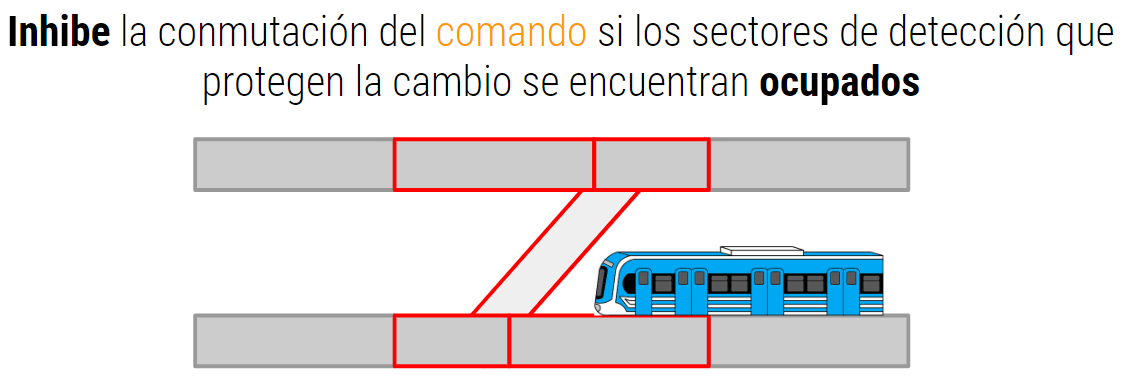
\includegraphics[width=1\textwidth]{Figuras/ocupacion}
        \centering\caption{Bloqueo de máquina de cambios por ocupación de secciones adyacentes.}
        \label{fig:ACG_ocupacion}
    \end{figure}

	La funcionalidad implementada radica en inhibir la conmutación de la máquina de cambios si alguna de las secciones de vías próximas al cambio de vías se encuentra ocupada. De esta manera, se garantiza que la posición del cambio de vías se mantendrá al detectar una formación aproximándose y no se permitirá su conmutación hasta que la formación se encuentre completamente alejada una distancia de seguridad. 
	\subsection{Requerimiento de rutas y bloqueo de cambios en ruta}

\lipsum[1]
    \begin{figure}[!h]
        \centering
        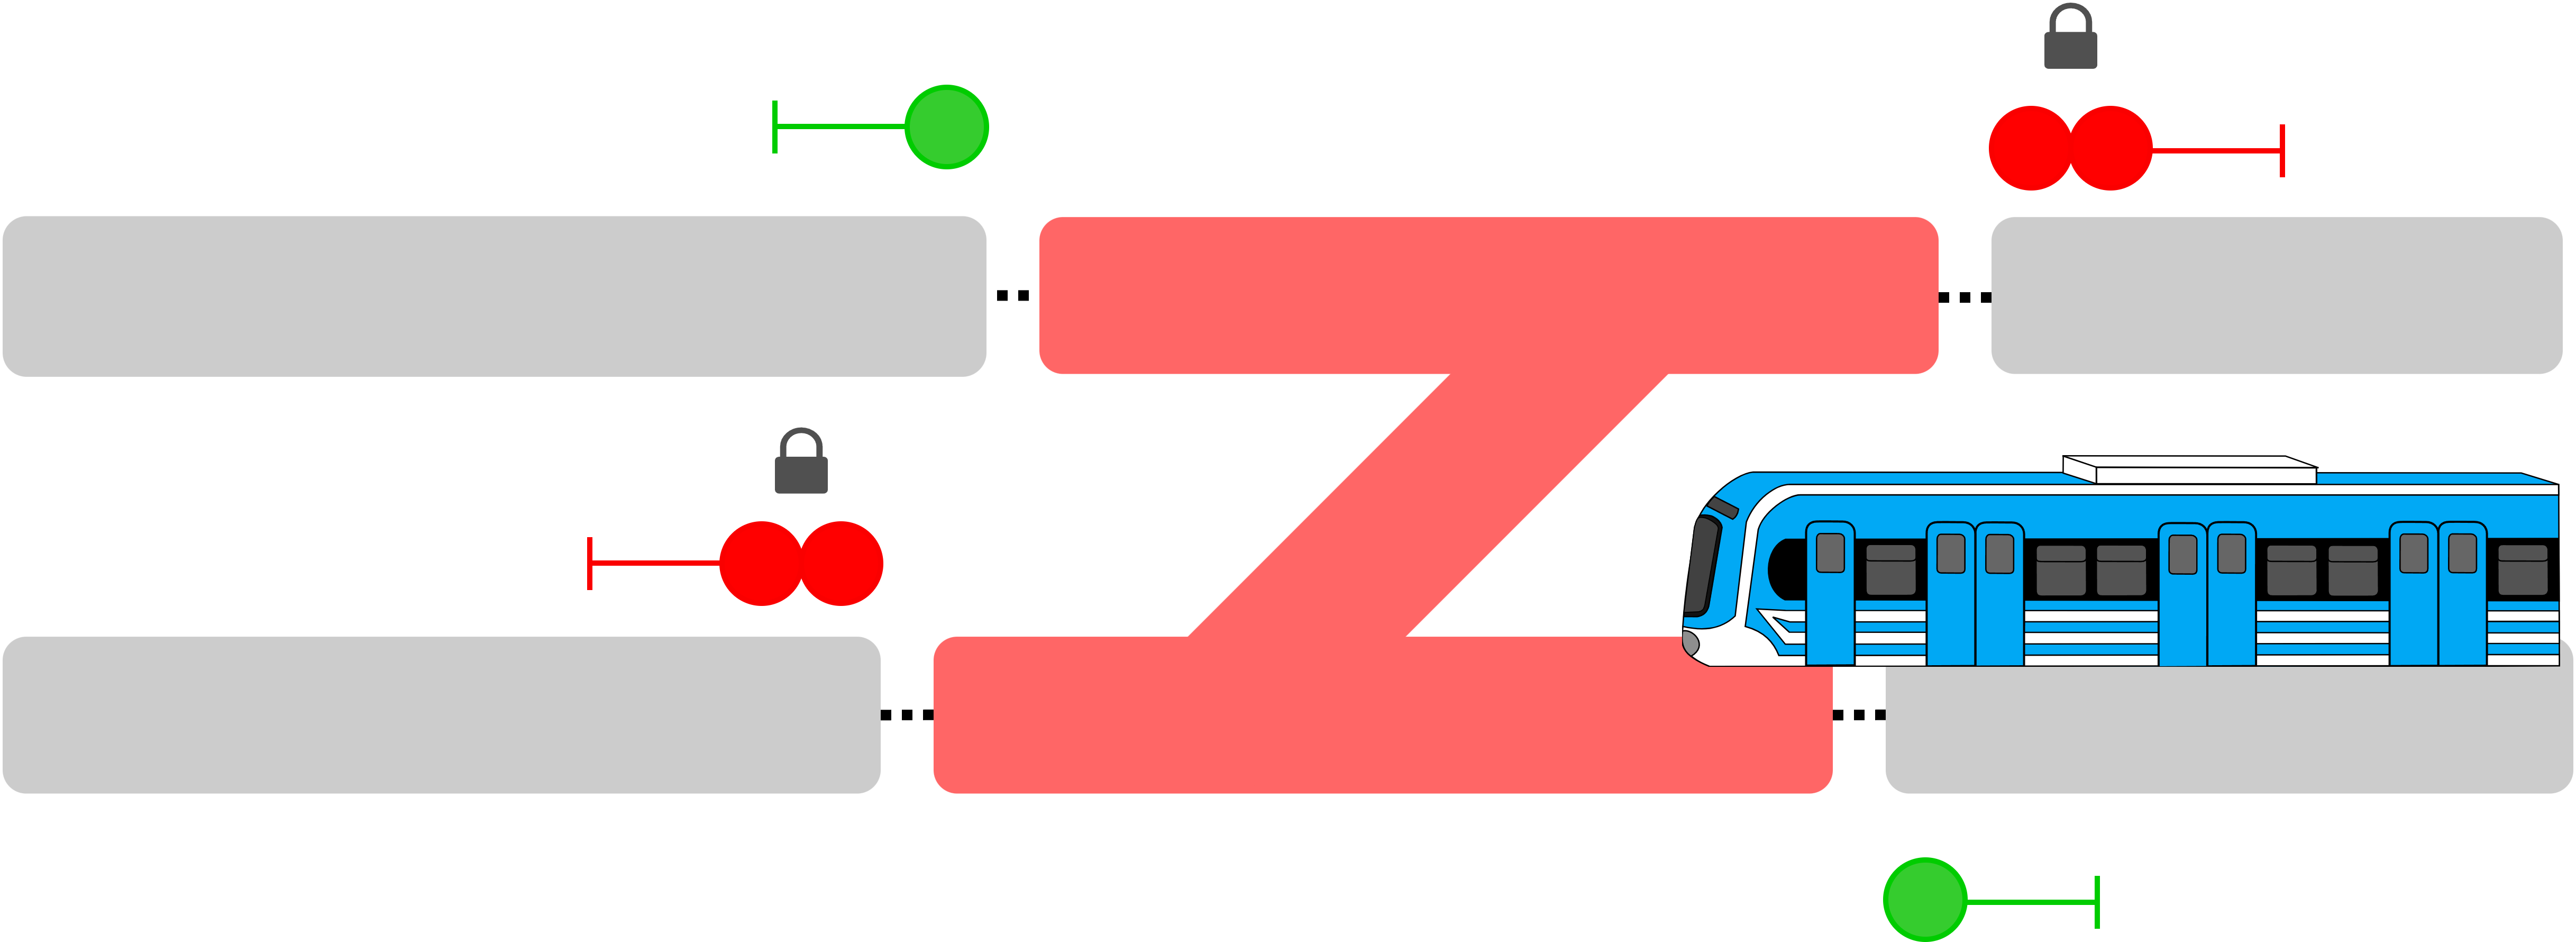
\includegraphics[width=1\textwidth]{Figuras/bloqueo_rutas}
        \centering\caption{XXXXX.}
        \label{fig:ocupacion_1}
    \end{figure}
\lipsum[1]
	\subsection{Protección por aproximación en cancelación de ruta}

	\label{sec:function_3}
	
	La distancia de frenado es un aspecto esencial a considerar cuando una ruta en curso es cancelada. La ruta en cuestión debe seguir protegida durante un tiempo de seguridad.
	
	La Figura \ref{fig:ACG_aproximacion_1} introduce el caso de una formación que tenía una ruta aprobada (aspecto verde) que comenzaba en la sección violeta y abarcaba toda la sección naranja. Por seguridad, ambos cambios de vías fueron bloqueados y sus respectivas señales contrarias fueron forzadas a aspecto rojo y bloqueadas.

    \begin{figure}[!h]
        \centering
        
\includegraphics[width=1\textwidth]{Figuras/aproximacion_1}
        \centering\caption{Formación aproximándose al inicio de la ruta.}
        \label{fig:ACG_aproximacion_1}
    \end{figure}
    
    Mientras la formación se encuentra en movimiento, el operador solicitó la cancelación de la ruta, cambiando el aspecto de la señal a rojo, tal como se visualiza en la Figura \ref{fig:ACG_aproximacion_2}. La formación quizás no tenga el tiempo ni la distancia suficiente para detenerse antes de la señal, por lo que se presentan dos escenarios. 
    
    \begin{figure}[!h]
        \centering
        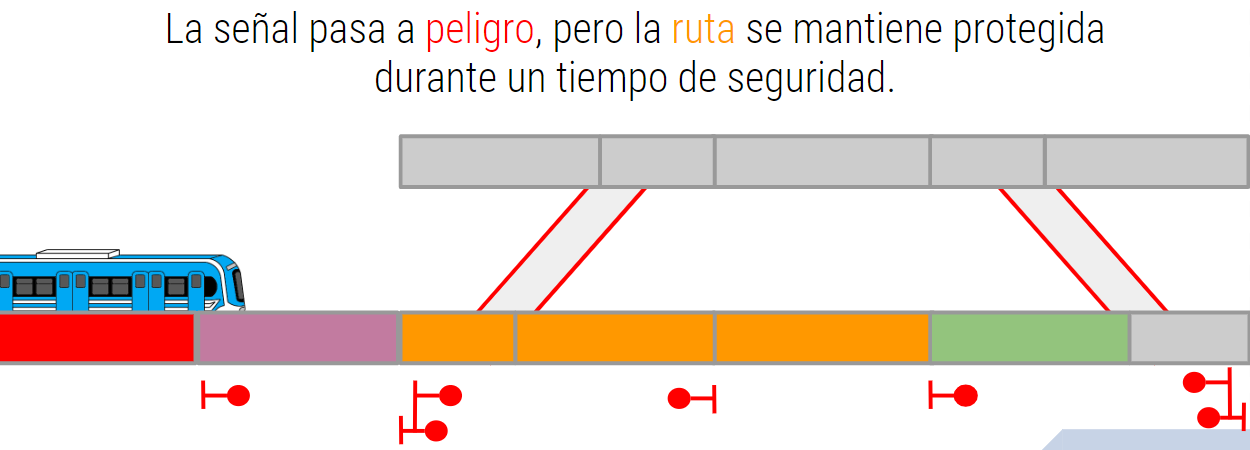
\includegraphics[width=1\textwidth]{Figuras/aproximacion_2}
        \centering\caption{La ruta es cancelada mietnras la formación se aproxima.}
        \label{fig:ACG_aproximacion_2}
    \end{figure}
    
    El primer escenario es el mas favorable: la formación se detiene previo a la señal de peligro y se inicia un contador. Al cumplirse el tiempo de seguridad, las secciones asociadas a la ruta cancelada son liberadas. Lo mismo sucede con los cambios de vías y las señales conflictivas. Este tiempo otorgado permite comprobar que la formación efectivamente se detuvo antes de proceder con la liberación de los elementos ferroviarios para que puedan ser utilizados por otra ruta.
    
    \begin{figure}[!h]
        \centering
        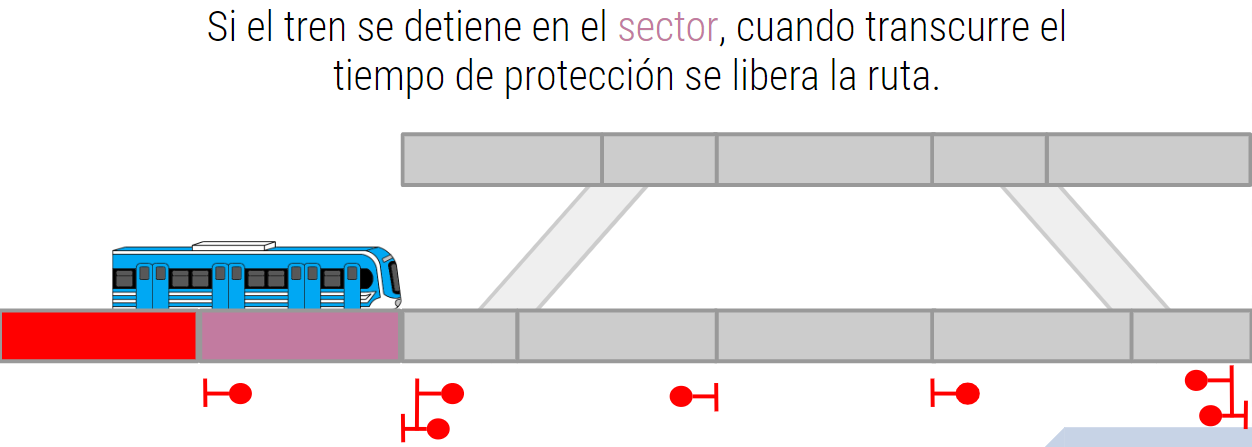
\includegraphics[width=1\textwidth]{Figuras/aproximacion_3}
        \centering\caption{La formación se detiene exitosamente previo a la señal de peligro.}
        \label{fig:ACG_aproximacion_3}
    \end{figure}
    
	En el segundo escenario, la formación no logra detenerse previo a la señal de peligro, tal como se ilustra en la Figura \ref{fig:ACG_aproximacion_4}. Entonces, el sistema de enclavamiento no solamente no libera las secciones pertenecientes a la ruta cancelada, sino que también bloquea las próximas secciones, al no poder estimar cual será la distancia final de frenado de la formación.

    \begin{figure}[!h]
        \centering
        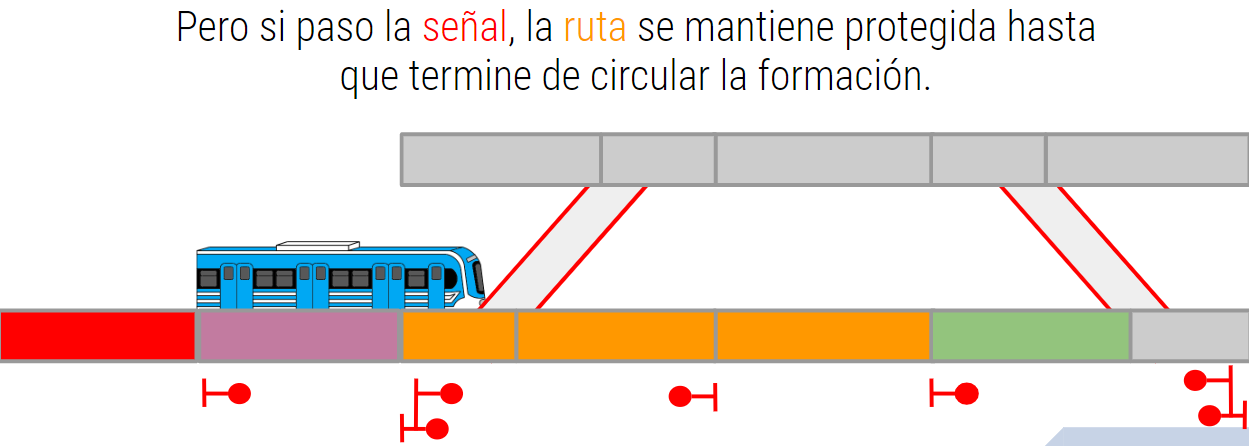
\includegraphics[width=1\textwidth]{Figuras/aproximacion_4}
        \centering\caption{La formación no se detiene previo a la señal de peligro.}
        \label{fig:ACG_aproximacion_4}
    \end{figure}
    
	Las secciones y elementos ferroviarios próximos se mantienen protegidos y enclavados hasta que la ruta se concluya, aún habiendo sido cancelada. Al finalizar la ruta, el sistema de enclavamiento liberará las secciones y elementos ferroviarios próximos al comprobarse que la formación se detuvo previo a la señal de finalización de la ruta.
	
	\subsection{Protección por solape}

	Si una formación no detiene su marcha antes de una señal de peligro, el sistema de enclavamiento debe bloquear las secciones pertenecientes a esa ruta y la próxima, junto con la infraestructura asociado. La Figura \ref{fig:ACG_solape_1} ilustra este suceso, donde una formación ingresa a la sección violeta pasando una señal a peligro, sin tener la autorización requerida. A diferencia de la protección por aproximación, donde una formación no logra detenerse antes de ingresar a una ruta cancelada con poca anticipación, la protección por solape se ocupa de proteger la infraestructura en el caso de que la formación ingrese a una ruta que jamás fue habilitada.

    \begin{figure}[!h]
        \centering
        \includegraphics[width=1\textwidth]{Figuras/solape}
        \centering\caption{Formación ignora señal a peligro y se activa la protección por solape.}
        \label{fig:ACG_solape_1}
    \end{figure}
    
    Automáticamente, las secciones de la próxima ruta (coloreadas en naranja) son bloqueadas, a la vez que los cambios de vías cercanos y todas las señales tanto consecutivas como contrarias o convergentes. El bloqueo se removerá una vez que la formación se detenga en la próxima señal a peligro, luego de un tiempo de seguridad.
	\subsection{Doble recubrimiento}
	\label{sec:function_5}
	
	Para evitar que una formación colisione con otra formación que se encuentre detenida más adelante en la misma vía o circulando a menor velocidad, el sistema de enclavamiento deberá controlar las señales entre ambas para regular la velocidad y distancia entre ellas. Tal como se explicó en la Sección \ref{sec:signals}, las señales pueden presentar diferentes aspectos. Cada aspecto determinará un rango de velocidad permitido, siendo rojo el mas restrictivo. La Figura \ref{fig:ACG_recrubrimiento_1} ilustra el comportamiento del señalamiento cuando dos formaciones circulan en el mismo sentido, separadas por una distancia de seguridad.
	
	\begin{figure}[!h]
		\centering
		\includegraphics[width=1\textwidth]{Figuras/recubrimiento}
		\centering\caption{Protección por doble recubrimiento.}
		\label{fig:ACG_recrubrimiento_1}
	\end{figure}
	
	La formación que circula por detrás (formación A en la Figura \ref{fig:ACG_recrubrimiento_1}) se encuentra frente a una señal de aspecto verde, por lo
	que puede continuar su marcha sin restricciones, siempre y cuando su velocidad sea menor a la velocidad máxima permitida en la red ferroviaria. Si la formación A reduce la distancia a la formación B, pasará a estar regida por una señal de aspecto amarillo. Si esto sucediera, la formación A deberá disminuir su velocidad para volver a situarse dentro de una sección verde. Lo mismo ocurriría si la formación A alcanzara una señal de aspecto doble amarillo, indicada mediante la señal naranja en la Figura 3.8. En este caso dado que la distancia entre formaciones es aún menor, deberá reducirse aún más la velocidad.
	
	Si la formación A continúa con una mayor velocidad que la formación B, la distancia entre ambas se reducirá y el señalamiento que la formación A tiene en su camino le impondrá velocidades más y más reducidas, hasta que la distancia entre ambas formaciones se incremente a un valor seguro.
		
	Debido al bloqueo por ocupación, todas las secciones ocupadas por una formación presentan una señal a peligro (roja). Inmediatamente detrás de cada formación se genera una secuencia de señales denominada doble recubrimiento. Si la formación avanza y cambia de sección, las señales de protección cambiarán su aspecto acorde al movimiento de la formación, de forma tal que siempre la sección donde está la formación tenga su señal de protección en rojo, la sección anterior en amarillo, la sección anterior en doble amarillo y la sección anterior en verde. Si no hay ninguna formación en la sección anterior a la que tiene su señal en verde, entonces esa sección también tendrá su señal en verde, lo mismo que todas las secciones anteriores, hasta que haya una formación que ocupe una sección, en cuyo caso esa sección estará en rojo y la secuencia de doble recubrimiento se repetirá también detrás de esa formación.
	 
	La cantidad de señales y la secuencia de aspectos variará según el operador de la red, las normas locales o nacionales. Algunos países como el Reino Unido \cite{UK} utilizan la secuencia rojo-doble amarillo-amarillo-verde (Figura \ref{fig:uk_signalling}) y esta es la secuencia de aspectos que implementa el ACG en este trabajo, aunque cabe aclarar que el ACG puede modificarse para implementar otras secuencias. 
	
	\begin{figure}[!h]
		\centering
		\includegraphics[width=0.5\textwidth]{Figuras/semaforo2}
		\centering\caption{Protección por doble recubrimiento.}
		\label{fig:uk_signalling}
	\end{figure}
	
	En las etapas iniciales del proyecto la única herramienta de visualización era Design4Rail \cite{DESIGN4RAIL}. Esta herramienta solamente puede representar señales de un aspecto y, al no tener todavía implementado el AGG, no era posible representar señales de doble aspecto amarillo. Es por esa razón que el RNA reemplazó la señal doble amarilla por una señal naranja. Este reemplazo también es realizado por el ACG al implementar las señales en VHDL. El proyecto se encontraba en estado muy avanzado cuando se diseñó el AGG, por lo que se mantuvo que todas las señales son de un único aspecto. En este trabajo, por lo tanto, siempre se representará mediante una señal naranja a una señal doble amarilla.
	
	
	%Ya que Design4Rail \cite{DESIGN4RAIL}, el software utilizado para visualizar el señalamiento al inicio del proyecto, solo puede representar señales de un aspecto, en la Figura \ref{fig:ACG_recrubrimiento_1} se reemplazó la señal doble amarilla por una señal naranja. En este trabajo siempre se representará mediante una señal naranja a una señal doble amarilla.

	
	
	\subsection{Liberación secuencial}
	\label{sec:ACG_liberacion}
	
	Esta claro que las rutas conflictivas no pueden ser habilitadas a la vez, pero existen algunas rutas que son parcialmente conflictivas solamente, que comparten una parte de la infraestructura y no toda. La implementación de la liberación secuencial aumenta la flexibilidad en la asignación y habilitación de rutas, mejorando la logística permita por el sistema de enclavamientos. En la Figura \ref{fig:ACG_secuencial_1} se ilustra una formación que iniciará una ruta ya habilitada, para lo cual ya han sido bloqueadas las secciones (coloreadas en naranja) y la infraestructura (coloreadas en rojo).
	
	 \begin{figure}[!h]
	     \centering
	     \includegraphics[width=1\textwidth]{Figuras/secuencial_1}
	     \centering\caption{Formación iniciando una ruta ferroviaria.}
	     \label{fig:ACG_secuencial_1}
	 \end{figure}
 
	Al ocupar las secciones de vías, debido al bloqueo por ocupación, la señal de inicio de la ruta pasa a peligro y se bloquea la sección consecutiva a la ruta (coloreado en naranja), debido a la protección por solape. Esto se ilustra en la Figura \ref{fig:ACG_secuencial_2}.
	
	\begin{figure}[!h]
    	 \centering
	     \includegraphics[width=1\textwidth]{Figuras/secuencial_2}
    	 \centering\caption{Formación activando el bloqueo por ocupación y el bloqueo por solape.}
    	 \label{fig:ACG_secuencial_2}
	\end{figure}
 
 	Una vez que la formación desocupa las secciones de vías asociadas al cambio de vías anterior, el sistema de enclavamientos libera inmediatamente toda la infraestructura asociada, como se ilustra en la Figura \ref{fig:ACG_secuencial_3}. A la vez, el sistema de enclavamientos debe esperar a que se cumpla el plazo de seguridad antes de liberar la infraestructura posterior al fin de la ruta. Solamente son liberadas las secciones y señales que ya no son conflictivas.
	   
	\begin{figure}[!h]
	  \centering
	  \includegraphics[width=1\textwidth]{Figuras/secuencial_3}
	  \centering\caption{Liberación secuencial de la infraestructura por detrás de la formación.}
	  \label{fig:ACG_secuencial_3}
	\end{figure}
 
 	Transcurrido el tiempo de seguridad, el sistema de enclavamientos libera las secciones, cambios de vías, señales y toda infraestructura posterior al fin de la ruta, tal como se ilustra en la Figura \ref{fig:ACG_secuencial_4}.

	 \begin{figure}[!h]
	     \centering
	     \includegraphics[width=1\textwidth]{Figuras/secuencial_4}
	     \centering\caption{Liberación secuencial de la infraestructura por delante de la formación.}
	     \label{fig:ACG_secuencial_4}
	 \end{figure}
	    
	El ACG implementa estas funcionalidades de seguridad para cada sistema de enclavamientos generado. 
	
	En las siguientes secciones se profundizará en la implementación de cada uno de los módulos del sistema y su comportamiento dinámico. 
    \section{Arquitectura del sistema}

	Cada módulo del sistema fue implementado con máquinas de estado finitas	con camino de datos (FSMD, del inglés Finite State Machine with Data path), que son máquinas de estado finitas (FSM, del inglés Finite State Machine) y circuitos
	secuenciales y combinacionales que constituyen el camino de datos. Utilizar una FSMD aporta un mayor control del diseño a bajo nivel, una mayor portabilidad y un mas eficiente uso de los recursos de la plataforma electrónica.
	
	Una FSMD, cómo la ilustrada en la Figura \ref{fig:FSMD}, posee dos partes diferenciadas: el camino de control y el camino de datos. El camino de control se compone de una FSM que, según las entradas de control y el estado interno que posee, genera señales internas que controlan los circuitos secuenciales del camino de datos. Estos, a su vez, contienen los bloques que procesan las entradas y actúan sobre las salidas.
	
	\begin{figure}[H]
		\centering
		\includegraphics[width=1\textwidth]{Figuras/FSMD.png}
		\centering\caption{Diagrama en bloques  de una FSMD genérica.}
		\label{fig:FSMD}
	\end{figure}
	
	El ACG generará automáticamente cada FSMD en función de los elementos detectados en la red de grafos. Es decir, el modelado de cada elemento será una plantilla que contemplará todos los casos posibles, con todas las entradas y salidas posibles, pero solo se implementarán las funcionalidades que cada elemento particular requieran. De esta manera, será posible optimizar los recursos a la vez que se valida cada elemento una única vez, como un objeto genérico.
	
	Los elementos ferroviarios a ser modelados por el ACG son los que denominaremos elementos dinámicos. Es decir, todo elemento ferroviario que posea algún estado susceptible de modificarse en función de algún evento o del tiempo. Estos elementos dinámicos pueden adoptar los siguientes estados:
	
	\begin{itemize}
		\item Circuitos de vía: ocupados, desocupados.
		\item Rutas: no solicitadas, solicitadas.
		\item Señales: rojo, doble amarillo, amarillo, verde
		\item Pasos a nivel: barrera baja, barrera alta.
		\item Cambios de vías simples: posición normal, posición reversa.
		\item Cambios de vías dobles: posición doble normal, posición doble reversa, posición normal reversa, posición reversa normal.
		\item Cambios de vias en tijeras: posición normal, posición reversa.
	\end{itemize}
	
	Internamente, el sistema contemplará que algunos elementos pueden admitir estados de transición. Estos estados son producto del tiempo que requiere un actuador para completar las comandos que la FPGA envía. No obstante, los estados de transición solo serán tolerados un tiempo determinado, pasado el cuál se asumirá que la orden no fue completada y se abortará la ejecución de la ruta solicitada.
	
	La arquitectura general del sistema generado por el ACG se ilustra en la Figura \ref{fig:GeneralSystem}. El módulo \textit{Detector} recibe las tramas en formato serie, comprueba su integridad y en caso de que los datos contengan solamente caracteres válidos los entrega al módulo \textit{Decoder}. El módulo \textit{Decoder} toma esos datos y los paraleliza para entregarlos al módulo \textit{Network} en la entrada que corresponda a cada dato. El módulo \textit{Network} es la implementación de la red de grafos generada por el RNA. 
	
	\begin{figure}[H]
		\centering
		\includegraphics[width=1\textwidth]{Figuras/Arq_general.png}
		\centering\caption{Arquitectura general del sistema generado por el ACG.}
		\label{fig:GeneralSystem}
	\end{figure}
	
	El módulo \textit{Encoder} toma las salidas generadas por el módulo \textit{Network}, las agrupa apropiadamente y se las suministra al módulo] \textit{Printer}. El módulo \textit{Printer} transforma cada elemento de la señal en un caracter imprimible para enviar a la UART. Finalmente, el módulo \textit{Selector} se usa exclusivamente a los fines de comprobar el correcto funcionamiento de la comunicación serie, puenteando a todos los otros módulos.
	
	La descripción del sistema se realizará desde sus módulos mas externos, que implementan la comunicación del sistema: los módulos de UART, Detector, Decoder, Encoder y Printer. De forma tal de entender en alto nivel como es el proceso de comunicación hacia y desde la FPGA, para luego abordar el núcleo del sistema de enclavamiento. cuya complejidad es mucho mayor.		
	
	\subsection{Modulo UART}
\label{sec:UART}
	Si consideramos la lista de elementos dinámicos y cada estado que pueden admitir, es claro que la cantidad de señales sobrepasaría por mucho la limitada cantidad de puertos que una FPGA pueda proveer. Por ejemplo, si se considera un sistema ferroviario como el presentado en la Figura \ref{fig:bypass_1}, que por comodidad para el lector se copia en la Figura \ref{fig:bypass_3}, seria necesario mas de 25 pines de la FPGA entre entradas y salidas, lo que implicaría que para ese sistema tan simple se requeriría utilizar una FPGA de tamaño medio o grande. Esto implica que ese enfoque dificultaría la implementación del sistema de enclavamiento de redes ferroviarias de mayor tamaño.
	
	\begin{figure}[H]
		\centering
		\includegraphics[width=1\textwidth]{Figuras/bypass}
		\centering\caption{Topología de derivación ferroviaria.}
		\label{fig:bypass_3}
	\end{figure}
	
	Es por eso que se decidió que la FPGA mediante la cual se implemente el sistema de enclavamiento debe recibir y transmitir la información a la cabina de señalamiento en formato serie. El uso de comunicación serie para la implementación del sistema es apropiado, ya que otros sistemas ferroviarios utilizan comunicación serie, como por ejemplo RS-485 o MVB en las redes de comunicación de trenes (TCN, del inglés \textit{Train Communication Network}) \cite{TCN}. La comunicación a implementar entre el sistema de enclavamiento y la cabina de señalamiento deberá ser flexible para ser utilizada en diferentes implementaciones con menor o mayor cantidad de elementos ferroviarios.
	
	En la Figura \ref{fig:GeneralCom} se presenta la propuesta de conexión de la FPGA con una computadora externa, que para el desarrollo y prueba de la solución hará las veces de la cabina de señalamiento. En la Figura \ref{fig:GeneralCom} también se representan los módulos internos de comunicación. La UART (del inglés \textit{Universal Asynchronous Receiver-Transmitter}), junto con las memorias FIFO (del inglés \textit{First-In First-Out}), se utilizan para implementar el intercambio de las tramas de datos entre la FPGA y la computadora.
	
	\begin{figure}[H]
		\centering
		\includegraphics[width=0.7\textwidth]{Figuras/UART_module.png}
		\centering\caption{Conexión entre la FPGA y una computadora externa.}
		\label{fig:GeneralCom}
	\end{figure}
	
	El módulo de recepción (UART RX), que se ilustra en la Figura \ref{fig:GeneralCom}, es el encargado de procesar cada bit recibido con un baudrate preestablecido y almacenar cada bit en la FIFO RX. Al completarse un byte de datos, será enviado al sistema de enclavamientos, junto con una serie de pulsos para indicar cuándo deben ser leídos. El sistema de enclavamientos esperará a tener la cantidad de bytes necesarios (definidos por el ACG) para empezar a procesar la trama. Luego, el sistema de enclavamientos devolverá una nueva trama de bytes a la FIFO TX. Finalmente la nueva trama será enviada al módulo de transmisión (UART TX) que enviará la información bit a bit, con el mismo baudrate que fue recibido.
	
	La implementación de los módulos de transmisión y recepción de la UART es invariante para cada locación, es decir, los recursos asignados serán los mismos, cualquiera sea el tamaño del sistema a implementar. Los módulos de memorias FIFO, en cambio, dependen de las características y del tamaño del sistema. Locaciones mas complejas tendrán valores de N y M mayores y, por lo tanto, requerirán FIFOs mas grandes. 
	
	En la Figura \ref{fig:Stream} se ilustra el formato definido para las tramas de entrada y salida. La trama tendrá un tamaño de entrada N y de salida M, con N igual que M. La cantidad de cada elemento ferroviario es definida por el RNA y el orden de los elementos es fijo y definido en el ACG. Los elementos que no existan en la locación analizada tendrán paquetes de datos de largo nulo. Además, la trama tendrá un caracter delimitador de entrada y de salida ($<$ y $>$ respectivamente). Todos los elementos de la trama serán hexadecimales en formato ASCII, para poder ser interpretados fácilmente en una terminal y ser menos susceptibles a errores por alteraciones en algún bit aleatorio.
	
	\begin{figure}[H]
		\centering
		\includegraphics[width=1\textwidth]{Figuras/Tramas.png}
		\centering\caption{Tramas de datos y paquete de datos.}
		\label{fig:Stream}
	\end{figure}
	
	El largo de la trama de entrada y de salida queda definido por la Ecuación \ref{eq:StreamLength_in}. 
	
	\begin{equation} 
		\label{eq:StreamLength_in}
		\text{N} = 1\text{byte} (\text{N}_{NET}+\text{N}_{\text{RTS}}+\text{N}_{\text{LCB}}+\text{N}_{\text{SSW}}+\text{N}_{\text{SCR}}\text{N}_{\text{SIG}}+\text{N}_{\text{DSW}})
	\end{equation}
	
	Cada elemento dinámico requiere un sólo caractér hexadecimal para definir su estado utilizando sus 4 bits. Los 2 bits menos significativos definen el estado (\textit{STATE} en Figura \ref{fig:Stream}). Por ejemplo, la posición de un cambio de vías o el aspecto de una señal. Los 2 bits mas significativos definen el enclavamiento del elemento dinámico (\textit{LOCK} en la Figura \ref{fig:Stream}). El parámetro \textit{Lock} puede tomar tres valores: '00' para elementos disponibles, '01' para elementos que han sido reservados por una ruta pero aún no han sido enclavados y '10' para elementos enclavados.
	
	En la Figura \ref{fig:Stream_ejemplo1} se ilustran dos tramas recibidas en el caso de una topología ferroviaria que será explicada en profundidad en la Sección \ref{sec:ejemplo_1}, y que a modo de referencia se presenta en la Figura \ref{fig:EJ1_2_B}. La primer trama de datos representa el estado del sistema de enclavamiento cuando no se han solicitado rutas y la segunda ilustra una ruta pedida y habilitada. Ambas tramas corresponden a la misma topología ferroviaria y cuentan con 11 netElements, 21 rutas, 23 señales, 2 pasos a nivel, 5 cambios de vías y los correspondientes tags iniciales y finales.
	
	\begin{figure}[H]
		\centering
		\includegraphics[width=1\textwidth]{Figuras/Trama_ejemplo.png}
		\centering\caption{Tramas de datos y paquete de datos.}
		\label{fig:Stream_ejemplo1}
	\end{figure}
	
	En la primer trama se pueden apreciar: 11 secciones de vías sin ocupar (todos los valores en 1), 21 rutas sin solicitar (todos los valores en 0), 23 señales de las cuales podemos destacar 14 señales rojas (valores en 0), 4 señales naranjas (valores en 1), 3 señales amarillas (valores en 2) y 2 señales verdes (valores en 3). Además, la trama describe dos pasos a nivel con el brazo de barrera en alto (todos los valores en 1) y 5 cambios de vías, 3 de ellos en posición normal (valores en 0) y 2 en posición reversa (valores en 1). Debido que no existen rutas solicitadas ni habilitadas en esta trama (todos los valores en 0), todos los elementos tienen sus valores de LOCK en '00', lo que indica que se encuentran disponibles para ser enclavados por la ruta correspondiente.

	En la segunda trama, en cambio, se puede apreciar que el primer netElement (ne1) es representado con un 8 (1000), lo cual significa que se encuentra enclavado (10) y ocupado (00). Los netElements ne9 y ne15 son representados con un 9 (1001), ya que también se encuentran enclavados (10), pero no han sido ocupados (01). Además, la ruta 12 es representada con un 7 (0111), el estado de liberación secuencial (que será explicado en la Sección \ref{sec:ACG_rts}). Los semáforos que presentan valores superiores a 4 (0100) son aquellos que se encuentran reservados y los que presentan valores superiores a 8 (1000) se encuentran enclavados. En este caso, el semáforo S22 se representa con un 7 (0111, verde y reservado) y el semáforo T05 se representa con un 8 (1000, rojo y enclavado). Finalmente, los cambios de vías pares se encuentran en posición normal y los impares en posición reversa. En el caso del cambio de vías sw04, el valor 9 representa un cambio de vías enclavado en posición reversa y el cambio de vías sw07, el valor 8 representa un cambio de vías enclavado en posición normal.
	
	\begin{figure}[H]
		\centering
		\includegraphics[width=1\textwidth]{resultados-obtenidos/ejemplo1/images/1_original.png}
		\centering\caption{Topología ferroviaria del ejemplo 1.}
		\label{fig:EJ1_2_B}
	\end{figure}
	
	
	
	
	
	
	%11111111111000000000000000000000101203210000000000120301110010
    %81191119111000000000000700000000171203210000000810120301190080
	
	
	%Con este criterio de diseño, en todos los demás casos, la FIFO de salida tendrá el mismo tamaño que la FIFO de entrada o a lo sumo será 50 \% menor, lo que representa un ahorro de 25 \% de los recursos estimados. Por ejemplo, si se necesita que la entrada tenga 15 bits y la salida 7 bits y se le asignara el mismo tamaño a ambas FIFOs; tanto la FIFO de entrada como la de salida necesitarán 16 bits cada una, dando un total de 32 bits. Pero si se aplica el criterio de tamaños desacoplados, entonces para la FIFO de salida podrían asignarse solamente 8 bits, dando un total de 24 bits, un 25 \% menos que los 32 bits que necesitaría si ambas FIFOs quedaran definidas según los datos de la entrada.
	\subsection{Módulo Detector}
	\label{sec:detector}
	
	El módulo \textit{detector} es el encargado de detectar el inicio y final de cada trama, validando que el contenido de la misma tenga N caracteres, conforme al formato de trama expuesto en la Sección \ref{sec:UART}. A medida que la validación tiene lugar, los caracteres ASCII son convertidos en valores booleanos (\textit{std\_logic}) dentro de un vector de elementos booleanos llamado \textit{packet}[N] (\textit{std\_logic\_vector} de N elementos). El diagrama de bloques de las máquinas de estado finitas con camino de datos se muestra en la Figura \ref{fig:Detector_module}.
	
	\begin{figure}[H]
		\centering
		\includegraphics[width=1\textwidth]{Figuras/Detector_module.png}
		\centering\caption{FSMD del módulo \textit{Detector}.}
		\label{fig:Detector_module}
	\end{figure}
	
	En cada pulso de reloj (\textit{clk\_i}), el módulo UART envía un caracter por medio de la señal \textit{r\_data} (8 bytes) y un pulso (\textit{r\_available}) para informar que un nuevo dato ha sido enviado. El pulso de reloj es utilizado principalmente en el módulo \textit{Counter\_0\_to\_N}, cuyo parámetro N ya ha sido calculado por el ACG previo a generar el código y es la cantidad de caracteres que serán enviados a continuación del caracter de inicio. El proceso de detección y validación de la trama recibida se describe el diagrama de estados de la Figura \ref{fig:Detector_FSMD}.
	
	\begin{figure}[H]
		\centering
		\includegraphics[width=0.8\textwidth]{Figuras/Detector_FSMD.png}
		\centering\caption{Diagrama de estados del módulo \textit{Detector}.}
		\label{fig:Detector_FSMD}
	\end{figure}
	
	El módulo \textit{Detector} inicia por detecto en el estado \textit{start}, aguardando por el caracter de inicio de trama '$<$'. Al recibir el caracter de inicio de trama, el módulo transiciona al estado \textit{reading}. En el estado \textit{reading} se recibirán solamente los caracteres ASCII '0' y '1'. Si al terminar de recibir N caracteres, el próximo caracter no es el de fin de trama '$>$' entonces se transiciona al estado \textit{error}, se reinician las variables auxiliares, la trama se descarta y se vuelve al estado \textit{start}.
	
	Si el próximo caracter luego de leer N valores ASCII '0' y '1' es el caracter de fin de trama '$>$', entonces el módulo transiciona al estado \textit{final}, donde se da por válida la trama y se habilita su envío al módulo \textit{decoder}, para volver al estado \textit{start} a la espera de un nuevl caracter de inicio de trama, reiniciando todas las variables auxiliares.
	
	Internamente se tienen diversas variables auxiliares para controlar si se han recibido los delimitadores y si la cantidad recibida es correcta. Eso cobra gran importancia al realizar los ensayos, porque se puede diferenciar rápidamente la fuente de posibles errores.
	\subsection{Módulo Decoder}
	\label{sec:decoder}
	
	El módulo \textit{Decoder} (ver Figura \ref{fig:GeneralSystem}) es el encargado de demultiplexar la trama \textit{packet}[N] ya validada por el módulo \textit{Detector}. El módulo \textit{Decoder} recibe el vector de elementos booleanos \textit{packet}[N] y la señal \textit{process} que indica cuando puede iniciar el proceso de demultiplexación. La salida serán todos los vectores de estado de los elementos ferroviarios. El diagrama de bloques de la máquinas de estado finitas con camino de datos se muestra en la Figura \ref{fig:Decoder_module}. En este caso particular, no se cuenta con una máquina de estados, ya que la demultiplexación se realiza directamente.
	
	\begin{figure}[H]
		\centering
		\includegraphics[width=1\textwidth]{Figuras/Decoder_module.png}
		\centering\caption{FSMD del módulo \textit{Decoder}.}
		\label{fig:Decoder_module}
	\end{figure}
	
	 La porción de \textit{packet}[N] correspondiente a cada vector será en función de la cantidad de elementos de cada tipo presentes en la locación. Esto ya fue calculado previamente por el ACG y explicado en la Sección \ref{sec:UART} al definir el formato de la trama. Si la cantidad de un cierto elemento ferroviario es mayor que uno, el ACG implementará el estado de ese elemento con un vector hexadecimal del tamaño adecuado. Si solo existe un elemento ferroviario de ese tipo, el ACG implementará un escalar hexadecimal. Si no existiese ningún elemento ferroviario en la locación, el ACG no implementará ninguna de las funcionalidades relativas a dicho elemento, optimizando el uso de recursos en la FPGA.
	\subsection{Módulo Encoder}
	\label{sec:encoder}
	
	El módulo \textit{Encoder} (ver Figura \ref{fig:GeneralSystem}) es el encargado de multiplexar los vectores de estado provenientes del módulo \textit{Network} y reconstruir una nueva trama, esta vez sin los valores de ocupación de vías por ser de sólo lectura. Esta nueva trama será \textit{packet}[N], junto con la señal \textit{processed} para indicar al módulo \textit{Printer} que la trama está completa y lista para ser transmitida. El diagrama de bloques de las máquinas de estado finitas con camino de datos se muestra en la Figura \ref{fig:Encoder_module}.
	
	\begin{figure}[H]
		\centering
		\includegraphics[width=1\textwidth]{Figuras/Encoder_module.png}
		\centering\caption{FSMD del módulo \textit{Encoder}.}
		\label{fig:Encoder_module}
	\end{figure}
	
	Al igual que la demultiplexación que realiza el módulo \textit{Decoder}, la multiplexación se basa en la cantidad de elementos ferroviarios de cada tipo, calculdos por el ACG al definir la trama tal cual fue explicado en la Sección \ref{sec:UART}. Los elementos inexistentes en la locación no serán tenidos en cuenta para formar la nueva trama, reduciendo el tamaño de la misma al mínimo.
	\subsection{Módulo Printer}
	\label{sec:printer}
	
	El módulo Printer (ver Figura \ref{fig:GeneralSystem}) realiza la conversión de cada elemento de un vector de M elementos hexadecimales (\textit{packet}[M], M elementos de 4 bits) en caracteres hexadecimales (1 byte). Cada elemento del vector es analizado en cada ciclo de reloj (clk\_i) y demultiplexado, de manera tal de convertir un elemento por vez, para luego enviar el byte correspondiente al módulo UART para su posterior transmisión al exterior. El diagrama de bloques de la máquina de estados finitos con camino de datos se muestra en la Figura \ref{fig:Printer_module}.
	
	\begin{figure}[H]
		\centering
		\includegraphics[width=1\textwidth]{Figuras/Printer_module.png}
		\centering\caption{FSMD del módulo \textit{Printer}.}
		\label{fig:Printer_module}
	\end{figure}
	
	En cada ciclo de reloj el módulo \textit{Printer} demultiplexa el vector \textit{packet}[M] para obtener un elemento lógico que procesar, según el valor del contador vigente, que se incrementa en cada ciclo, hasta un máximo de M-1. Si el elemento \textit{packet}[i] es un valor hexadecimal, se enviará un byte equivalente en ASCII. Por ejemplo, se enviará un byte equivalente al 'A' ASCII si el elemento \textit{packet}[i] es una 'A' hexadecimal.
	
	Cada dos ciclos de reloj el módulo \textit{Printer} genera un pulso para habilitar el envío del último byte generado. Junto con el caracter se envía la señal \textit{wr\_uart} para indicarle a la UART que ese dato debe ser guardado en la FIFO de salida y la señal \textit{processed} para indicarle al módulo \textit{Detector} que se pueden procesar nuevas tramas. El ciclo de procesamiento de la trama a transmitir se describe el diagrama de estados de la Figura \ref{fig:Printer_FSMD}.
	
	\begin{figure}[H]
		\centering
		\includegraphics[width=0.8\textwidth]{Figuras/Printer_FSMD.png}
		\centering\caption{Diagrama de estados del módulo \textit{Printer}.}
		\label{fig:Printer_FSMD}
	\end{figure}
	
	El módulo \textit{Printer} inicia por detecto en el estado \textit{restart}, a la espera de recibir la señal \textit{process} del módulo \textit{Encoder}. Se tienen dos estados (\textit{cycle\_1} y \textit{cycle\_2}) para generar el pulso de reloj necesario para mantener sincronizadas las tramas. Cuando el contador haya recorrido los M elementos de \textit{packet}[M], el módulo vuelve al estado \textit{restart}, para esperar una nueva señal \textit{process} para volver a procesar una nueva trama de datos.
	
	Si la trama recibida es incorrecta, o si ya fue impresa, entonces la señal \textit{process} será '0' y el modulo \textit{Printer} dejará de enviar datos a la UART. Si la señal \textit{process} mantiene un estado lógico positivo, el proceso de impresión continuará hasta que la UART indique que no pueda recibir mas datos o que alguna etapa previa informe de algún error en el proceso.
	\subsection{Módulo Selector}
	\label{sec:selector}
	
	Se añadió el módulo \textit{Selector} (ver Figura \ref{fig:GeneralSystem}) para poder facilitar el testeo de la comunicación serial al permitir anular la totalidad del sistema de enclavamiento. De esta manera, es posible validar la lectura, detección y escritura de tramas en bucle en forma independiente al sistema de enclavamiento. Esta funcionalidad es habilitada cambiando la posición de un switch físico de la FPGA y se desactiva invirtiendo su posición. El diagrama de bloques de la máquina de estados finitos con camino de datos diseñado para lograr este objectivo se muestra en la Figura \ref{fig:Selector_module}.
	
	\begin{figure}[H]
		\centering
		\includegraphics[width=0.55\textwidth]{Figuras/Selector_module.png}
		\centering\caption{FSMD del módulo \textit{Selector}.}
		\label{fig:Selector_module}
	\end{figure}
	\subsection{Modulo Network}

El módulo \textit{Network} es el encargado de instanciar todos los elementos ferroviarios presentes en la red de grafos generada por el RNA e interconectarlos como ésta indica. Es el módulo que mas recursos de la FPGA utiliza y donde más se hace énfasis en el uso óptimo de los recursos. Se prioriza la máxima descentralización posible de los módulos instanciados internamente, de forma tal que cada uno de ellos solo dependa de la mínima cantidad necesaria de módulos, evitando conexiones innecesarias. El diagrama de bloques de las máquinas de estado finitas con camino de datos diseñado para lograr este objetivo se muestra en la Figura \ref{fig:Network_module}.

\begin{figure}[H]
	\centering
	\includegraphics[width=1\textwidth]{Figuras/Network_module.png}
	\centering\caption{FSMD del módulo \textit{Network}.}
	\label{fig:Network_module}
\end{figure}

Los módulos de \textit{NetElements}, \textit{Routes} y \textit{Signals} son obligatorios ya que se encuentran presentes en la mínima red ferroviaria aceptada por el RNA. En cambio, los módulos de \textit{SingleSwitches}, \textit{DoubleSwitches}, \textit{ScissorCrossings} y \textit{LevelCrossings} son opcionales y dependen de que existan en la locación. Es decir, si un elemento ferroviario no existe, no solamente no serán instanciado por el ACG, sino que tampoco se generarán archivos que definan sus módulos, señales auxiliares que los interconecten a otros módulos ni tampoco entradas o salidas en otros módulos, destinados a este elemento. De esta manera, se reduce la complejidad del sistema enormemente al implementar solamente los puertos, señales, módulos y conexiones que serán utilizados por el sistema de enclavamiento.

Para garantizar la descentralización de la red, a todos los elementos ferroviarios con entidad física, es decir, todos los mencionados menos las rutas que son entidades abstractas, se les implementa la propiedad de enclavamiento. El enclavamiento de un elemento puede presentar tres estados, tal como se describe en la Tabla \ref{Tab:interlock_states}.

	\begin{table}[!h]
	{
		\caption{Estados de enclavamiento de cada elemento ferroviario.}
		\label{Tab:interlock_states}
		\centering
		\resizebox{1\textwidth}{!}{
		\begin{tabular}{ p{5cm} p{4cm} p{4cm} }
			\hline	
			Liberado & Reservado & Enclavado \\	
			\hline
			Solicitado por cualquier ruta u opera de forma automática.& 
			Operado solamente por la ruta que lo reservó.&
			Depende de sí mismo y de la ruta que lo enclavó.\\
			\hline
		\end{tabular}
		}
	}
	\end{table}

Todo elemento se encuentra por defecto en el estado liberado y puede ser solicitado por cualquier ruta. Tan pronto una ruta envía el comando de reserva al elemento, pasa a estar en estado reservado y ninguna otra ruta podrá hacer uso de este elemento. Finalmente, si la ruta ha podido reservar todos los elementos necesarios para cumplir las condiciones para ser habilitada, enviará la señal de enclavamiento a todos los elementos involucrados, evitando que puedan ser comandados por otras rutas. Esto incluye tanto a la ocupación de vías (\textit{NetElements}) como a las señales (\textit{Signals}), pasando por todos los cambios de vías (\textit{SingleSwitches}, \textit{DoubleSwitches} y \textit{ScissorCrossings}) y barreras de pasos a nivel (\textit{LevelCrossings}). De esta manera el ACG se asegura que cada elemento sea controlado por una única ruta por vez o de forma automática si ninguna ruta demanda su uso.

Para generalizar y modelizar el comportamiento dinámico del enclavamiento los elementos ferroviarios recurrimos a las redes de Petri \cite{Paper_64,Paper_65,Paper_88,Paper_94,Paper_95,Paper_123,Paper_196}. Una red de Petri es la representación gráfica de un modelo matemático de autómatas concurrente. Las mismas están formadas por lugares (el estado), las transiciones que concentran las condiciones para pasar de un lugar a otro y los arcos que conectan lugares y transiciones. Las redes de Petri puede poseer uno o mas tokens que representan en que estado se encuentra el sistema. Algunas redes de Petri admiten mas de un token por red, o incluso mas de un token por lugar. En el caso del sistema de enclavamiento se definieron solamente redes de Petri con un único token por red, siendo que el sistema solo puede adoptar un estado en cada momento. En la Figura \ref{fig:Interlocking_petri} se visualiza el modelo matemático del enclavamiento de un elemento ferroviario genérico.

\begin{figure}[H]
	\centering
	\includegraphics[width=0.7\textwidth]{Figuras/INT_petri}
	\centering\caption{Red de Petri del modelo dinámico de enclavamiento de elementos ferroviarios genéricos.}
	\label{fig:Interlocking_petri}
\end{figure}

La transición de un elemento ferroviario del estado liberado a reservado no solo puede darse por el pedido expreso de una ruta que lo solicite, sino también de facto al ocuparse los netElements cercanos al elemento, lo cual inicia lo que se denomina 'bloqueo por ocupación' (ver Sección XXX). Esto protege al sistema al impedir que otras rutas soliciten un cambio de estado de un elemento que esta siendo usado por una formación que no ha solicitado ningún permiso, reduciendo el riesgo de accidentes por descarrillamiento o colisión. La red de Petri también deja explícito la inclusión de un timeout para las reservas, con un valor por defecto de 7 segundos, configurable por el usuario. De no cumplirse que el comando y la indicación coincidan dentro del tiempo estipulado, el elemento es liberado, siempre que no se encuentren formaciones cercanas. Las transición de reserva a enclavamiento requiere que tanto el comando como la indicación coincidan y que la ruta solicite el enclavamiento al haber confirmado que todas las condiciones de ruta se han cumplido y es inminente su habilitación. El elemento ferroviario deja de estar enclavado cuando la ruta lo solicita expresamente, momento en el cuál pasa a estar liberado para que otras rutas puedan usarlo.

A diferencia de los módulos explicados en secciones anteriores, donde cada módulo era instanciado una vez, los módulos que modelan elementos ferroviarios, con entidad física o abstracta, son instanciados tantas veces como unidades de éstos existan. Es por eso que, en las siguientes secciones, hablaremos de módulos genéricos a la hora de describir cada módulo. Estos módulos genéricos presentarán todas las entradas, salidas y funcionalidades que pueden tener, de ser requeridas. 

Es trabajo del ACG determinar cuales de ellas deben ser implementadas y cuales no. Por ejemplo, si una ruta A requiere que una barrera X se encuentre baja, pero no tiene requerimientos respecto a las posiciones de los cambios porque la ruta A no los utiliza, entonces el ACG instanciará el módulo de la ruta A considerando en las entradas y salidas los estados de la barrera X y los comandos para operarla, intercontando el módulo de ruta A con el módulo de la barrera ferroviaria X. En cambio, el ACG no implementará ningún puerto destinado a los cambios de vías ni lo considerará en las funcionalidades del módulo de ruta A. De igual manera, el ACG conectará los estados de ocupación de vías correspondientes solamente a los módulos de los elementos ferroviarios que los necesitan y no la totalidad del vector de datos.

\input{ACG/arquitectura/levelCrossings}
\input{ACG/arquitectura/singlesSwitches}
\input{ACG/arquitectura/doubleSwitches}
\input{ACG/arquitectura/scissorCrossings}
\input{ACG/arquitectura/netElements}
\input{ACG/arquitectura/signals}
\input{ACG/arquitectura/routes}    
    \section{Redundancia}

\lipsum[1]

\begin{figure}[!h]
        \centering
        \includegraphics[width=1\textwidth]{Figuras/antagonica}
        \centering\caption{XXXXX.}
        \label{fig:redundancia_1}
    \end{figure}

\lipsum[1]

    \section{Validacion de la implementacion}

\lipsum[1]

\newpage
\chapter{Resultados obtenidos}
	\label{sec:resultados}
\lipsum[1]

\begin{figure}[H]
	\centering
	\includegraphics[width=1\textwidth]{example-image}
	\centering\caption{FPGA.}
	\label{fig:LABEL}
\end{figure}


\section{Ejemplo 1}

    \lipsum[1]

    \begin{figure}[h]
        \centering
        \includegraphics[width=1\textwidth]{resultados-obtenidos/ejemplo1/images/1_original.png}
        \centering\caption{Señalamiento original del ejemplo 1.}
        %\label{fig:LC_P2}
    \end{figure}

    \begin{figure}[h]
        \centering
        \includegraphics[width=1\textwidth]{resultados-obtenidos/ejemplo1/images/1_empty.png}
        \centering\caption{Topología ferroviaria del ejemplo 1 sin señalamiento.}
        %\label{fig:LC_P2}
    \end{figure}

    \begin{figure}[h]
        \centering
        \includegraphics[width=1\textwidth]{resultados-obtenidos/ejemplo1/images/1_step1.png}
        \centering\caption{Señalamiento generado por el RNA para proteger el fín de vía.}
        %\label{fig:LC_P2}
    \end{figure}

    \begin{figure}[h]
        \centering
        \includegraphics[width=1\textwidth]{resultados-obtenidos/ejemplo1/images/1_step2.png}
        \centering\caption{Señalamiento generado por el RNA para proteger las junturas.}
        %\label{fig:LC_P2}
    \end{figure}

    \begin{figure}[h]
        \centering
        \includegraphics[width=1\textwidth]{resultados-obtenidos/ejemplo1/images/1_step3.png}
        \centering\caption{Señalamiento generado por el RNA para proteger plataformas y cruces de vía.}
        %\label{fig:LC_P2}
    \end{figure}

    \begin{figure}[h]
        \centering
        \includegraphics[width=1\textwidth]{resultados-obtenidos/ejemplo1/images/1_step4.png}
        \centering\caption{Señalamiento generado por el RNA para proteger las máquinas de cambios.}
        %\label{fig:LC_P2}
    \end{figure}

    \begin{figure}[h]
        \centering
        \includegraphics[width=1\textwidth]{resultados-obtenidos/ejemplo1/images/1_RNA.png}
        \centering\caption{Señalamiento generado y simplificado por el RNA.}
        %\label{fig:LC_P2}
    \end{figure}
    
    \subsection{Señalamiento original}

    El señalamiento diseñado en forma manual por el autor de esta tesis para la topología de la Figura \ref{fig:EJ1_1} se ilustra en la Figura \ref{fig:EJ1_2}. Se observa que incluye señales de parada próximas a los finales de vías absolutos (S18, S19, S20), señales de partida en las plataformas (S04, S06, S08, S09), señales de protección antes de cada paso a nivel (S04, S05), señales de maniobras antes de converger en una vía principal (S03, S08) y señales múltiples para cambios de vías divergentes (S01, S17, S10, S07), entre varias otras señales. Estas señales permiten definir hasta un máximo de 14 rutas, todas ellas detalladas en la Tabla \ref{Tab:tabla_original_1}
    
    \begin{figure}[H]
    	\centering
    	\includegraphics[width=1\textwidth]{resultados-obtenidos/ejemplo1/images/1_original.png}
    	\centering\caption{Señalamiento original del ejemplo 1.}
    	\label{fig:EJ1_2}
    \end{figure}
    
    En una primera inspección, se puede comprobar que todos los elementos ferroviarios son alcanzados por al menos una de las rutas, en al menos una dirección. Además, todos los cambios de vías son utilizados, de forma simple o compuesta. 
    
    \begin{table}[H]
        {
        \caption{Tabla de enclavamiento original del ejemplo 1.}
        \label{Tab:tabla_original_1}
        \centering
        \resizebox{1\textwidth}{!}{
            \begin{tabular}{ c c c c c c c }
                \hline	
                    Ruta & Inicio & Final & Cambio & Plataforma & Cruce & netElement \\	
                \hline
                    R$_{01}$  & S$_{05}$ & S$_{06}$ & - & Plat$_{11}$ & Lc$_{06}$ & ne$_{14}$\\
                    R$_{02}$  & S$_{06}$ & S$_{20}$ & - & - & - & ne$_{14}$\\
                    R$_{03}$  & S$_{09}$ & S$_{18}$ & - & - & - & ne$_{13}$\\
                    R$_{04}$  & S$_{13}$ & S$_{12}$ & Sw$_{13}^{N}$ & - & - & ne$_{23}$-ne$_{12}$\\
                    R$_{05}$  & S$_{16}$ & S$_{02}$ & Sw$_{12}^{N}$ & - & - & ne$_{22}$-ne$_{08}$\\
                    R$_{06}$  & S$_{07}$ & S$_{10}$ & Sw$_{06}^{N}$ & - & - & ne$_{02}$-ne$_{12}$\\
                    R$_{07}$  & S$_{07}$ & S$_{09}$ & Sw$_{06}^{R}$ & Plat$_{13}$ & Lc$_{08}$ & ne$_{02}$-ne$_{13}$\\
                    R$_{08}$  & S$_{10}$ & S$_{14}$ & Sw$_{13}^{N}$ & - & - & ne$_{12}$-ne$_{23}$\\
                    R$_{09}$  & S$_{10}$ & S$_{02}$ & Sw$_{12}^{R}$+Sw$_{13}^{R}$ & - & - & ne$_{12}$-ne$_{24}$-ne$_{08}$\\
                    R$_{10}$  & S$_{01}$ & S$_{17}$ & Sw$_{04}^{N}$ & - & - & ne$_{01}$-ne$_{08}$\\
                    R$_{11}$  & S$_{01}$ & S$_{19}$ & Sw$_{04}^{R}$+Sw$_{07}^{N}$ & - & - & ne$_{01}$-ne$_{15}$\\
                    R$_{12}$  & S$_{01}$ & S$_{05}$ & Sw$_{04}^{R}$+Sw$_{07}^{R}$ & - & - & ne$_{01}$-ne$_{14}$\\
                    R$_{13}$  & S$_{17}$ & S$_{15}$ & Sw$_{12}^{N}$ & - & - & ne$_{08}$-ne$_{22}$\\
                    R$_{14}$  & S$_{17}$ & S$_{12}$ & Sw$_{12}^{R}$+Sw$_{13}^{R}$ & - & - & ne$_{08}$-ne$_{24}$-ne$_{12}$\\    
                \hline
            \end{tabular}
        }
     }
    \end{table}
    
    Algunas rutas abarcan mas de un \textit{netElement}, como por ejemplo la ruta R14 que comienza en la señal S17 y finaliza en la señal S12, atraviesa los \textit{netElements} ne8, ne24 y ne12, y utiliza los cambios de vías Sw12 y Sw13, ambos en posición reversa.

    \subsection{Señalamiento generado por el RNA}

    \lipsum[1]
    
    \begin{table}[!h]
        {
        \caption{Tabla de enclavamiento del ejemplo 1 generada por el RNA.}
        \label{Tab:tabla_generated_1}
        \centering
        \resizebox{1\textwidth}{!}{
            \begin{tabular}{ c c c c c c c }
                \hline	
                    Ruta & Inicio & Final & Cambio & Plataforma & Cruce & netElement \\	
                \hline
                    R$_{01}$  & T$_{02}$ & P$_{20}$ & - & Plat$_{13}$ & Lc$_{08}$ & ne$_{13}$\\
                    R$_{02}$  & T$_{04}$ & X$_{16}$ & - & Plat$_{11}$ & - & ne$_{14}$\\
                    R$_{03}$  & T$_{06}$ & C$_{29}$ & - & - & - & ne$_{15}$\\
                    R$_{04}$  & J$_{11}$ & L$_{09}$ & - & - & - & ne$_{22}$\\
                    R$_{05}$  & J$_{12}$ & C$_{21}$ & Sw$_{12}^{N}$ & - & - & ne$_{22}$-ne$_{08}$\\
                    R$_{06}$  & J$_{13}$ & C$_{25}$ & Sw$_{13}^{N}$ & - & Lc$_{08}$ & ne$_{23}$-ne$_{12}$\\
                    R$_{07}$  & X$_{15}$ & T$_{03}$ & - & Plat$_{11}$ & Lc$_{06}$ & ne$_{14}$\\
                    R$_{08}$  & X$_{16}$ & L$_{07}$ & Sw$_{04}^{R}$+Sw$_{07}^{R}$ & - & - & ne$_{14}$-ne$_{01}$\\
                    R$_{09}$  & P$_{20}$ & L$_{08}$ & Sw$_{06}^{R}$ & - & - & ne$_{13}$-ne$_{02}$\\
                    R$_{10}$  & C$_{21}$ & L$_{07}$ & Sw$_{04}^{N}$ & - & - & ne$_{08}$-ne$_{01}$\\
                    R$_{11}$  & S$_{22}$ & S$_{32}$ & Sw$_{04}^{N}$ & - & - & ne$_{01}$-ne$_{08}$\\
                    R$_{12}$  & S$_{22}$ & X$_{15}$ & Sw$_{04}^{R}$+Sw$_{07}^{R}$ & - & - & ne$_{01}$-ne$_{14}$\\
                    R$_{13}$  & S$_{22}$ & T$_{05}$ & Sw$_{04}^{R}$+Sw$_{07}^{N}$ & - & - & ne$_{01}$-ne$_{15}$\\
                    R$_{14}$  & C$_{25}$ & L$_{08}$ & Sw$_{06}^{N}$ & - & - & ne$_{12}$-ne$_{02}$\\
                    R$_{15}$  & S$_{27}$ & S$_{35}$ & Sw$_{06}^{N}$ & - & - & ne$_{02}$-ne$_{12}$\\
                    R$_{16}$  & S$_{27}$ & T$_{01}$ & Sw$_{06}^{R}$ & Plat$_{13}$ & Lc$_{08}$ & ne$_{02}$-ne$_{13}$\\
                    R$_{17}$  & C$_{29}$ & L$_{07}$ & Sw$_{04}^{R}$+Sw$_{07}^{N}$ & - & - & ne$_{15}$-ne$_{01}$\\
                    R$_{18}$  & S$_{32}$ & J$_{11}$ & Sw$_{12}^{N}$ & - & - & ne$_{08}$-ne$_{22}$\\
                    R$_{19}$  & S$_{32}$ & C$_{25}$ & Sw$_{12}^{R}$+Sw$_{13}^{R}$ & - & - & ne$_{08}$-ne$_{12}$\\
                    R$_{20}$  & S$_{35}$ & J$_{14}$ & Sw$_{13}^{N}$ & - & - & ne$_{12}$-ne$_{23}$\\
                    R$_{21}$  & S$_{35}$ & C$_{21}$ & Sw$_{12}^{R}$+Sw$_{13}^{R}$ & - & - & ne$_{12}$-ne$_{08}$\\
                \hline
            \end{tabular}
        }
     }
    \end{table}
    \subsection{Sistema generado por el ACG}
	\label{sec:EJEMPLO1_ACG}
	
	En base a la red de grafos, ilustrada en la Figura \ref{fig:EJ1_8}, el ACG determinó la cantidad de elementos ferroviarios de cada tipo, tal como puede visualizarse en el Código \ref{lst:EJ1_8}.
	
	\begin{lstlisting}[language = {}, caption = Cantidad de elementos a implementar por el ACG, label = {lst:EJ1_8}]
	n_netElements:11
	n_switch:5
	n_doubleSwitch:0
	n_borders:4
	n_buffers:3
	n_levelCrossings:2
	n_platforms:2
	n_scissorCrossings:0
	n_signals:23
	N : 62
	\end{lstlisting}
	
	El ACG genera, en el caso de este ejemplo, 80 archivos en formato VHDL, tal como se puede visualizar en la Figura \ref{fig:EJ1_ACG_1}. Podemos destacar de la Figura \ref{fig:EJ1_ACG_1} al archivo \textit{Arty\_Z7-10.XDC}, que define los pines de entrada y salida de la plataforma Arty Z7 10 y Arty Z7 20. Este archivo es provisto por Xilinx para esta familia de plataformas. En caso de utilizar otra plataforma, se deberá incluir el archivo XDC correspondiente. En ambos casos, cada desarrollador debe asignar manualmente los pines a cada puerto del sistema generado por el ACG.
	
	\begin{figure}[H]
		\centering
		\includegraphics[origin = c, width=1\textwidth]{resultados-obtenidos/ejemplo1/images/ACG_files}
		\centering\caption{Archivos generador por el ACG para el ejemplo 1.}
		\label{fig:EJ1_ACG_1}
	\end{figure}
	
	Además, podemos mencionar los archivos \textit{my\_package.VHDL} y \textit{flipFlop.VHDL}, ambos generados por el ACG. El primero es una librería que define todos los tipos de datos utilizados por el sistema, y el segundo es un flip-flop tipo D utilizado para generar la secuencia de shift registers necesarios para adaptar el clock de entrada a los diferentes dominios de clock necesarios para el timeout de cada elemento ferroviario.
	
	Los archivos restantes son archivos que definen los módulos de alto nivel explicados en la Sección \ref{sec:interlockingArch} o la representación en VHDL de cada elemento ferroviario explicado entre la Sección \ref{sec:ACG_lc} y la Sección \ref{sec:ACG_rts}. Por ejemplo, en base lo descrito en el Código \ref{lst:EJ1_8}, hay 23 señales ferroviarias y podemos visualizar en la Figura \ref{fig:EJ1_ACG_1} 23 archivos referidos a las señales ferroviarias: desde \textit{railwaySignal\_0} hasta \textit{railwaySignal\_22}.
	
	Cada ejemplo cuenta con su propia carpeta de principio a fin. Es decir, el archivo railML original, los archivos generados por el RNA y el código generado por el ACG se encuentran en carpetas individuales para cada ejemplo. Esto es una ventaja a la hora de mantener un orden pero una gran desventaja a la hora de sintetizar los proyectos en Vivado. Cada conjunto de archivos debería ser importado de manera individual, previa desvinculación de los archivos del proyecto anterior. Para solucionar este inconveniente se desarrolló el Código \ref{lst:EJ1_script}, que automatiza la importación y desvinculación de los archivos de cada ejemplo.
	
	
	\begin{lstlisting}[language = {bash}, caption = script.tcl, label = {lst:EJ1_script}]
set chosen 1

# Get a list of all design source files
set design_sources [get_files -of_objects [get_filesets sources_1]]

remove_files $design_sources

set base_folder_path "ROOT/GICSAFePhD/App/Layouts/Example_"
set folder_path "${base_folder_path}${chosen}/VHDL"

puts $folder_path

set files [glob -directory $folder_path *.vhd]

add_files -norecurse -scan_for_includes  $files

update_compile_order -fileset sources_1
update_compile_order -fileset sources_1

synth_design -rtl -rtl_skip_mlo -name rtl_1
	\end{lstlisting}
	
	El parámetro \textit{chosen} indica el número de ejemplo seleccionado, mientras que \textit{base\_folder\_path} es la ruta absoluta de los ejemplos, cuyas carpetas deben ser nombradas como \textit{Example\_}+\textit{chosen} para poder ser encontradas. El Código \ref{lst:EJ1_script} puede ser importado en Vivado desde \textit{Tools $>$ Custom Commands $>$ Customize Commands} como un archivo TCL (del inglés, Tool Command Language), que es el formato que define los comandos nativos de Vivado. Pueden importarse tantos archivos TCL como se deseen, uno por cada ejemplo a sintetizar. De esta manera, cada script aparecerá en la barra de acceso rápido de Vivado de forma independiente y se automatiza el proceso de sincronización de archivos.
	
	Una vez ejecutado el script, Vivado ordenará los archivos de forma jerárquica, como puede verse en la parte izquierda de la Figura \ref{fig:EJ1_ACG_Vivado} donde el módulo \textit{global} incluye todos los módulos que fueron detallados en la Sección \ref{sec:interlockingArch}. Podemos destacar al módulo \textit{network} que es instanciado 3 veces junto con el módulo \textit{voter}, al ser una redundancia 2oo3, tal fue explicado en la Sección \ref{sec:VHDL2oo3}. Cada una de las instancias del módulo \textit{network} contienen sus propias 62 instancias de los mismos módulos de cada elemento ferroviario ya que N, cantidad de elementos ferroviarios, es 62 en el Código \ref{lst:EJ1_8}.	
	
	\begin{figure}[H]
		\centering
		\includegraphics[origin = c, width=1\textwidth]{resultados-obtenidos/ejemplo1/images/ACG_vivado}
		\centering\caption{Interfaz del entorno de desarrollo Vivado para el ejemplo 1.}
		\label{fig:EJ1_ACG_Vivado}
	\end{figure}
	
	La parte derecha de la Figura \ref{fig:EJ1_ACG_Vivado} ilustra la representación en diagrama de bloques de uno de los módulos \textit{network} (los tres módulos tienen los mismos bloques). Puede apreciarse en esta ventana que existen 66 módulos interconectados de forma compleja utilizando 871 señales. Pero esto es solamente una porción del sistema generado por el ACG, de inspeccionar cada uno de los bloques es posible determinar que el ejemplo 1 utiliza 9517 sub módulos conectados automáticamente mediante 21899 señales, lo cual se aleja bastante de un desarrollo que pueda realizarse manualmente de forma trivial.
	
	Una vez que Vivado ha generado el diagrama de bloques ya tenemos la certeza de que el código VHDL ha pasado la prueba de sintaxis del entorno de desarrollo. A continuación, se deberá sintetizar e implementar el sistema para generar el bitstream que será utilizado para programar la FPGA. Durante el proceso de síntesis, Vivado busca la mejor forma de representar el código VHDL con compuertas lógicas, por lo que un código de mejor calidad brindará una representación en hardware lo mas fiel posible a lo buscado. Durante el proceso de implementación, en cambio, Vivado calcula si la representación con compuertas lógicas es posible de realizarse con la plataforma disponible. En este proceso influye no solamente la cantidad de compuertas disponibles sino también el tipo de compuertas. Si la plataforma no cuenta con la cantidad suficiente de compuertas A, entonces Vivado buscará la forma de reemplazar esa compuerta por otras compuertas B, C o D, que sean su equivalente lógico. Este proceso de reemplazo y/o simplificación puede llevar a que ambos procesos presenten discrepancias en la cantidad de elementos utilizados. 
	
	Los resultados de ambos procesos son detallados en la Tabla \ref{Tab:tabla_ACG_1}. Los porcentajes de uso son calculados por Vivado automáticamente, teniendo en cuenta que la plataforma Arty Z7 20 posee 53200 Look-Up-Tables (LUTs), 106400 Flip-Flops (FFs), 125 Pines de entrada y salida (IOs) y 32 Buffers (BUFGs), tal cómo se explicó en la Sección \ref{sec:AGG}. En este ejemplo, la cantidad de recursos utilizados es baja y el tiempo de síntesis e implementación es de 47 y 44 segundos, respectivamente.
	
	\begin{table}[H]
		{
			\caption{Síntesis e implementación del ejemplo 1 generado por el ACG.}
			\label{Tab:tabla_ACG_1}
			\centering
			%\small
			%\centering
			\begin{center}
				\resizebox{0.7\textwidth}{!}{
					\begin{tabular}{ c c c c }
						\hline	
						Recursos & Síntesis & Implementación & Uso \\	
						\hline
						LUT & 3457 & 3416 & 6.42/6.50\%\\
						FF & 3810 & 3813 & 3.58\%\\
						IO & 15 & 15 & 12.00\%\\
						BUFG & 3 & 3 & 9.38\%\\
						\hline
					\end{tabular}
				}
			\end{center}
		}    
	\end{table}
	
	
	
    \subsection{Validación del sistema de enclavamientos}

    Las 14 rutas del señalamiento original (Tabla \ref{Tab:tabla_original_1}) tienen 14 rutas equivalentes en el señalamiento generado por el RNA (Tabla \ref{Tab:tabla_generated_1}), tal como se puede visualizar en la Tabla \ref{Tab:tabla_validation_1}, generada automáticamente por el RNA.

    \begin{table}[H]
        {
        \caption{Equivalencias entre las rutas originales y las generadas por el RNA.}
        \label{Tab:tabla_validation_1}
        \centering
        %\small
            %\centering
            \begin{center}
            \resizebox{0.7\textwidth}{!}{
            \begin{tabular}{ c c c c }
                \hline	
                    Original & Señales & RNA & Señales \\	
                \hline
                    R$_{01}$ & S$_{05}$-S$_{06}$ & R$_{07}$ & X$_{15}$-T$_{03}$ \\
                    R$_{02}$ & S$_{06}$-S$_{20}$ & R$_{07}$ & X$_{15}$-T$_{03}$ \\
                    R$_{03}$ & S$_{09}$-S$_{18}$ & R$_{16}$ & S$_{27}$-T$_{01}$ \\
                    R$_{04}$ & S$_{13}$-S$_{12}$ & R$_{06}$ & J$_{13}$-C$_{25}$ \\
                    R$_{05}$ & S$_{16}$-S$_{02}$ & R$_{05}$ & J$_{12}$-C$_{21}$ \\
                    R$_{06}$ & S$_{07}$-S$_{10}$ & R$_{15}$ & S$_{27}$-S$_{35}$ \\
                    R$_{07}$ & S$_{07}$-S$_{09}$ & R$_{16}$ & S$_{27}$-T$_{01}$ \\
                    R$_{08}$ & S$_{10}$-S$_{14}$ & R$_{20}$ & S$_{35}$-J$_{14}$ \\
                    R$_{09}$ & S$_{10}$-S$_{02}$ & R$_{21}$ & S$_{35}$-C$_{21}$ \\
                    R$_{10}$ & S$_{01}$-S$_{17}$ & R$_{11}$ & S$_{22}$-S$_{32}$ \\
                    R$_{11}$ & S$_{01}$-S$_{19}$ & R$_{13}$ & S$_{22}$-X$_{15}$ \\
                    R$_{12}$ & S$_{01}$-S$_{05}$ & R$_{12}$ & S$_{22}$-T$_{05}$ \\
                    R$_{13}$ & S$_{17}$-S$_{15}$ & R$_{18}$ & S$_{32}$-J$_{11}$ \\
                    R$_{14}$ & S$_{17}$-S$_{12}$ & R$_{19}$ & S$_{32}$-C$_{25}$ \\   
                \hline
            \end{tabular}
            }
            \end{center}
        }    
    \end{table}
    
    Las rutas R1, R2, R3, R4, R7, R8, R9, R10, R13, R14 y R16 (Tabla \ref{Tab:tabla_generated_1}) generadas por el RNA que no tienen equivalencias en el señalamiento original (Tabla \ref{Tab:tabla_original_1}) se deben a que el RNA creó señales extras. Las señales T01, T02, T03, T04, T05 y T06 fueron creadas por el RNA para proteger los finales de vía absolutos, mientras que las señales L07, L08, L09 y L10 fueron creadas para proteger los finales de vías relativos. Estas nuevas señales constituyen nuevas rutas que permiten a las formaciones detenerse previo al final (relativo o absoluto) de la red ferroviaria, lo cual incrementa la seguridad y añade nuevas rutas en sentido contrario, mejorando la logística. Estos elementos ferroviarios no se encontraban protegidos en el señalamiento original.
    
    El señalamiento original carecía de señales protegiendo los finales de vía absolutos y relativos. No obstante, esto no se debe a un error en el diseño original, sino a que el diseño de señalamientos en la vida real se encuentra restringido por las necesidades particulares de cada locación, operador o leyes locales. Algunos operadores priorizarán tener rutas largas, dejando largas distancias sin señalamiento electrónico. Algunas normativas pueden indicar que la protección de ciertos elementos puede ser optativa. En el caso de los finales de vía pueden utilizarse señales lumínicas intermitentes que no son controladas por el señalamiento.
    
    En otros ejemplos el señalamiento original puede estar "incompleto", es decir, solo se consideraron las rutas en un sentido determinado, en base al uso que se le quería dar a ese señalamiento. El RNA, en cambio, siempre generará el señalamiento completo, que abarque la totalidad de la red ferroviaria ingresada, a menos que se seleccione la opción de señalamiento parcial, que respetará el sentido único de circulación que se defina en cada vía.    
    
    %TODO VALIDACION ALGORITMOS
    
    
    
    
    
\section{Ejemplo 2}

    \lipsum[1]
    
    \begin{figure}[h]
    	\centering
    	\includegraphics[width=1\textwidth]{Figuras/Graph_2}
    	\centering\caption{XXXX}
    	%\label{fig:LC_P2}
    \end{figure}
    
    \lipsum[1]

    \begin{figure}[h]
        \centering
        \includegraphics[width=1\textwidth]{resultados-obtenidos/ejemplo2/images/2_original.png}
        \centering\caption{Señalamiento original del ejemplo 2.}
        %\label{fig:LC_P2}
    \end{figure}

    \begin{figure}[h]
        \centering
        \includegraphics[width=1\textwidth]{resultados-obtenidos/ejemplo2/images/2_empty.png}
        \centering\caption{Topología ferroviaria del ejemplo 2 sin señalamiento.}
        %\label{fig:LC_P2}
    \end{figure}

    \begin{figure}[h]
        \centering
        \includegraphics[width=1\textwidth]{resultados-obtenidos/ejemplo2/images/2_step1.png}
        \centering\caption{Señalamiento generado por el RNA para proteger el fín de vía.}
        %\label{fig:LC_P2}
    \end{figure}

    \begin{figure}[h]
        \centering
        \includegraphics[width=1\textwidth]{resultados-obtenidos/ejemplo2/images/2_step2.png}
        \centering\caption{Señalamiento generado por el RNA para proteger las junturas.}
        %\label{fig:LC_P2}
    \end{figure}

    \begin{figure}[h]
        \centering
        \includegraphics[width=1\textwidth]{resultados-obtenidos/ejemplo2/images/2_step3.png}
        \centering\caption{Señalamiento generado por el RNA para proteger plataformas y cruces de vía.}
        %\label{fig:LC_P2}
    \end{figure}

    \begin{figure}[h]
        \centering
        \includegraphics[width=1\textwidth]{resultados-obtenidos/ejemplo2/images/2_step4.png}
        \centering\caption{Señalamiento generado por el RNA para proteger las máquinas de cambios.}
        %\label{fig:LC_P2}
    \end{figure}

    \begin{figure}[h]
        \centering
        \includegraphics[width=1\textwidth]{resultados-obtenidos/ejemplo2/images/2_RNA.png}
        \centering\caption{Señalamiento generado y simplificado por el RNA.}
        %\label{fig:LC_P2}
    \end{figure}
    
    \subsection{Señalamiento original}

    \lipsum[1]
    
    \begin{table}[H]
        {
        \caption{Tabla de enclavamiento original del ejemplo 2.}
        \label{Tab:tabla_original_2}
        \centering
        \resizebox{1\textwidth}{!}{
            \begin{tabular}{ c c c c c c c }
                \hline	
                    Ruta & Inicio & Final & Cambio & Plataforma & Cruce & netElement \\	
                \hline
                    R$_{01}$  & S$_{07}$ & S$_{11}$ & Sw$_{01}^{N}$ & - & - & ne$_{14}$-ne$_{16}$\\
                    R$_{02}$  & S$_{08}$ & S$_{11}$ & Sw$_{01}^{R}$ & - & - & ne$_{15}$-ne$_{16}$\\
                    R$_{03}$  & S$_{09}$ & S$_{12}$ & Sw$_{02}^{N}$ & - & - & ne$_{18}$-ne$_{16}$\\
                    R$_{04}$  & S$_{10}$ & S$_{13}$ & Sw$_{03}^{N}$ & - & - & ne$_{20}$-ne$_{19}$\\
                    R$_{05}$  & S$_{10}$ & S$_{12}$ & Sw$_{03}^{R}$+Sw$_{02}^{R}$ & - & - & ne$_{20}$-ne$_{17}$-ne$_{16}$\\  
                \hline
            \end{tabular}
        }
     }
    \end{table}
    \section{Señalamiento generado por el RNA}

	El RNA también exporta la misma información mostrada en el Código \ref{lst:EJ2_8} en una hoja de cálculo, similar a la que se visualiza en la Tabla \ref{Tab:tabla_generated_2}.   
    
    \begin{table}[H]
        {
        \caption{Tabla de enclavamiento del ejemplo 2 generada por el RNA.}
        \label{Tab:tabla_generated_2}
        %\centering
        \begin{center}
        \resizebox{0.8\textwidth}{!}{
            \begin{tabular}{ c c c c c c c }
                \hline	
                    Ruta & Inicio & Final & Cambio & Plataforma & Cruce & netElement \\	
                \hline
                    R$_{01}$  & T$_{02}$ & L$_{06}$ & Sw$_{03}^{N}$ & - & - & ne$_{19}$-ne$_{20}$\\
                    R$_{02}$  & C$_{13}$ & S$_{18}$ & Sw$_{01}^{N}$ & - & - & ne$_{14}$-ne$_{16}$\\
                    R$_{03}$  & B$_{14}$ & S$_{18}$ & Sw$_{01}^{R}$ & - & - & ne$_{15}$-ne$_{16}$\\
                    R$_{04}$  & S$_{15}$ & P$_{09}$ & Sw$_{01}^{N}$ & Plat$_{01}$ & Lc$_{01}$ & ne$_{16}$-ne$_{14}$\\
                    R$_{05}$  & S$_{15}$ & L$_{04}$ & Sw$_{01}^{R}$ & Plat$_{01}$ & Lc$_{01}$ & ne$_{16}$-ne$_{15}$\\
                    R$_{06}$  & C$_{17}$ & S$_{15}$ & Sw$_{02}^{N}$ & - & - & ne$_{18}$-ne$_{16}$\\
                    R$_{07}$  & S$_{18}$ & P$_{12}$ & Sw$_{02}^{N}$ & Plat$_{02}$ & Lc$_{01}$ & ne$_{16}$-ne$_{18}$\\
                    R$_{08}$  & S$_{18}$ & L$_{06}$ & Sw$_{02}^{R}$+Sw$_{03}^{R}$ & - & Lc$_{01}$ & ne$_{16}$-ne$_{20}$\\
                    R$_{09}$  & S$_{21}$ & S$_{15}$ & Sw$_{02}^{R}$+Sw$_{03}^{R}$ & - & - & ne$_{20}$-ne$_{16}$\\
                    R$_{10}$  & S$_{21}$ & T$_{01}$ & Sw$_{03}^{N}$ & - & - & ne$_{20}$-ne$_{19}$\\
                \hline
            \end{tabular}
        }
        \end{center}
     }
    \end{table}
    
    En una primera inspección podemos ver que el nuevo señalamiento tiene 10 rutas, versus las 5 rutas del señalamiento original (ver Tabla \ref{Tab:tabla_original_2}). Esto se debe a que todas las vías son consideradas de ambos sentidos por el RNA, lo cuál queda de manifiesto cuando se comprueba que todas las plataformas y cruces de vía son atravesados por al menos una ruta. 
    \subsection{Sistema generado por el ACG}

	En base a la red de grafos, ilustrada en la Figura \ref{fig:EJ2_8}, el ACG determinó la siguiente cantidad de elementos, tal puede visualizarse en el Código \ref{lst:EJ2_8}.
	
	\begin{lstlisting}[language = {}, caption = Cantidad de elementos a implementar por el ACG, label = {lst:EJ2_8}]
	n_netElements:7
	n_switch:3
	n_doubleSwitch:0
	n_borders:4
	n_buffers:1
	n_levelCrossings:1
	n_platforms:2
	n_scissorCrossings:0
	n_signals:12
	N : 45
	M : 38
	\end{lstlisting}
	
	El código VHDL generado por el ACG es importado en un proyecto de Vivado, donde es sintetizado e implementado para generar el bitstream que será utilizado para programar la FPGA. La cantidad de elementos de la FPGA utilizados por el sistema post-síntesis y post-implementación, así como el porcentaje de uso de la plataforma, son detallados en la Tabla \ref{Tab:tabla_ACG_2}.
	
	\begin{table}[H]
		{
			\caption{Síntesis e implementación del ejemplo 2 generado por el ACG.}
			\label{Tab:tabla_ACG_2}
			\centering
			%\small
			%\centering
			\begin{center}
				\resizebox{0.7\textwidth}{!}{
					\begin{tabular}{ c c c c }
						\hline	
						Recursos & Síntesis & Implementación & Uso \\	
						\hline
						LUT & 1881 & 1879 & 3.54\%\\
						FF & 2433 & 2433 & 2.29\%\\
						IO & 16 & 16 & 12.80\%\\
						BUFG & 1 & 1 & 3.13\%\\
						\hline
					\end{tabular}
				}
			\end{center}
		}    
	\end{table}
	
	En este ejemplo, la cantidad de recursos utilizados es baja y el tiempo de sintetización e implementación es de 34 y 35 segundos respectivamente.
    \subsection{Validacion del sistema}

\lipsum[1]

    \begin{table}[H]
        {
        \caption{Equivalencias entre las rutas originales y las generadas por el RNA.}
        \label{Tab:tabla_original_1}
        \centering
        %\small
            %\centering
            \begin{center}
            \resizebox{1\textwidth}{!}{
            \begin{tabular}{ c c c c }
                \hline	
                    Original & Señales & RNA & Señales \\	
                \hline
                    R$_{01}$ & S$_{07}$-S$_{11}$ & R$_{03}$ & B$_{14}$-S$_{18}$ \\
                    R$_{02}$ & S$_{08}$-S$_{11}$ & R$_{06}$ & C$_{17}$-S$_{15}$ \\
                    R$_{03}$ & S$_{09}$-S$_{12}$ & R$_{02}$ & C$_{13}$-S$_{18}$ \\
                    R$_{04}$ & S$_{10}$-S$_{13}$ & R$_{10}$ & S$_{21}$-S$_{15}$ \\
                    R$_{05}$ & S$_{10}$-S$_{12}$ & R$_{09}$ & S$_{21}$-S$_{15}$ \\
                \hline
            \end{tabular}
            }
            \end{center}
        }    
    \end{table}
    
    \lipsum[1]
\chapter{Ejemplo 3}

	\label{sec:ejemplo_3}
	
    \subsection{Topología ferroviaria original}

	El tercer ejemplo, ilustrado en la Figura \ref{fig:EJ3_1}, es una de los ejemplos provistos por railML.org llamado 'AdvancedExample'. Esta topología es de las mas complejas disponibles para analizar. Consiste en siete estaciones interconectadas por medio de variadas topologías ferroviarias que incluyen el uso de cambios de vías simples, dobles y en tijeras. También presenta varias playas de maniobras, curvas, pasos bajo nivel y sobre nivel. El objetivo de este ejemplo fue comprobar el funcionamiento del RNA con la topología mas compleja disponible, exigiendo al máximo al ACG y verificando la escalabilidad del sistema generado.
	
	\begin{figure}[h]
		\centering
		\includegraphics[width=1\textwidth]{resultados-obtenidos/ejemplo3/images/3_empty.png}
		\centering\caption{Topología ferroviaria del ejemplo 3 sin señalamiento.}
		\label{fig:EJ3_1}
	\end{figure}
	
	Debido a la alta complejidad de este ejemplo, no será posible referirse a detalles muy puntuales de la red, al ser demasiados y muy extensos. No obstante, se listarán cada una de las señales creadas en cada paso y se ilustrarán los resultados a la par del proceso. Se extraerán conclusiones generales del análisis y se dará un detalle pormenorizado de las diferencias entre el señalamiento original y el generado.

    \subsection{Señalamiento original}

    \lipsum[1]
    
    \begin{table}[H]
        {
        \caption{Tabla de enclavamiento original del ejemplo 3.}
        \label{Tab:tabla_original_3}
        \centering
        \resizebox{1\textwidth}{!}{
            \begin{tabular}{ c c c c c c c }
                \hline	
                    Ruta & Inicio & Final & Cambio & Plataforma & Cruce & netElement \\	
                \hline
                    R$_{01}$ & 68N1 & 69Va & - & - & Lc$_{01}$ & ne$_{7}$-ne$_{95}$\\
                    R$_{02}$ & 68N2 & 69Va & - & - & Lc$_{01}$ & ne$_{1}$-ne$_{95}$\\
                    R$_{03}$ & 69Va & 69A & - & - & - & ne$_{95}$-ne$_{59}$\\
                    R$_{04}$ & 69A & 69N2 & 69W$_{03}^{N}$ & Plat$_{09}$ & - & ne$_{59}$-ne$_{17}$\\
                    R$_{05}$ & 69A & 69N3 & 69W$_{03}^{R}$ & Plat$_{13}$ & - & ne$_{59}$-ne$_{77}$\\
                    R$_{06}$ & 69P2 & 68F & - & - & - & ne$_{17}$-ne$_{9}$\\
                    R$_{07}$ & 69B2 & 69P2 & Sw$_{06}^{N}$ & Plat$_{09}$ & - & ne$_{78}$-ne$_{17}$\\
                    R$_{08}$ & 69B2 & 69P3 & Sw$_{06}^{R}$+Sw$_{07}^{S}$ & Plat$_{13}$ & - & ne$_{78}$-ne$_{77}$\\
                    R$_{09}$ & 69B2 & 69P1 & Sw$_{06}^{R}$+Sw$_{07}^{T}$ & Plat$_{12}$ & - & ne$_{78}$-ne$_{21}$\\
                    R$_{10}$ & 69C & 69N1 & - & Plat$_{12}$ & - & ne$_{70}$-ne$_{21}$\\
                    R$_{11}$ & 69Vc1 & 69C & - & - & -  & ne$_{70}$-ne$_{70}$\\
                    R$_{12}$ & 69Vc & 69Vc1 & - & Plat$_{07}$ & - & ne$_{67}$-ne$_{70}$\\
                    R$_{13}$ & 70Va & 70A & - & - & -  & ne$_{103}$-ne$_{64}$\\
                    R$_{14}$ & 70N2 & 69Vc & - & - & -  & ne$_{23}$-ne$_{67}$\\
                    R$_{15}$ & 70N1 & 69Vc & - & - & - & ne$_{24}$-ne$_{67}$\\
                    R$_{16}$ & 70P1 & 72Va & - & - & - & ne$_{24}$-ne$_{44}$\\
                    R$_{17}$ & 70P2 & 72Va & - & - & - & ne$_{23}$-ne$_{44}$\\
                    R$_{18}$ & 70B & 70N2 & 70W$_{02}^{N}$ & Plat$_{05}$ & - & ne$_{26}$-ne$_{23}$\\
                    R$_{19}$ & 70B & 70N1 & 70W$_{02}^{R}$ & Plat$_{06}$ & - & ne$_{26}$-ne$_{24}$\\
                    R$_{20}$ & 70A & 70P1 & 70W$_{01}^{N}$ & Plat$_{06}$ & - & ne$_{64}$-ne$_{24}$\\
                    R$_{21}$ & 70A & 70P2 & 70W$_{01}^{R}$ & Plat$_{05}$ & - & ne$_{64}$-ne$_{23}$\\
                    R$_{22}$ & 69W04Y & 69N3 & - & Plat$_{13}$ & - & ne$_{14}$-ne$_{77}$\\
                    R$_{23}$ & 72Va & 72A & - & - & - & ne$_{44}$-ne$_{100}$\\
                    R$_{24}$ & 721 & S01 & - & - & - & ne$_{83}$-ne$_{32}$\\
                    R$_{25}$ & 723b & S01 & Sw$_{05}^{T}$ & - & - & ne$_{41}$-ne$_{32}$\\
                    R$_{26}$ & 723b & 72B & Sw$_{05}^{S}$ & - & - & ne$_{41}$-ne$_{100}$\\
                    R$_{27}$ & 722 & 72B & - & - & - & ne$_{29}$-ne$_{100}$\\
                    R$_{28}$ & S01 & 72B & - & - & - & ne$_{32}$-ne$_{100}$\\
                    R$_{29}$ & 69B1 & 69P3 & Sw$_{07}^{T}$ & Plat$_{13}$ & - & ne$_{94}$-ne$_{77}$\\
                    R$_{30}$ & 69B1 & 69P1 & Sw$_{07}^{S}$ & Plat$_{12}$ & - & ne$_{94}$-ne$_{21}$\\
                    R$_{31}$ & 72B & 70B & 71W$_{01}^{N}$ & - & - & ne$_{100}$-ne$_{26}$\\
                    R$_{32}$ & 69P3 & 68F & 69W$_{04}^{R}$ & - & - & ne$_{77}$-ne$_{9}$\\
                    R$_{33}$ & 69P1 & 70Va & - & - & - & ne$_{21}$-ne$_{103}$\\
                \hline
            \end{tabular}
        }
     }
    \end{table}
    
    \lipsum[1]
    \subsection{Generación de señalamiento paso a paso}
	
	Al ejecutar el RNA, primero detectará todos los \textit{netElements}, sus coordenadas iniciales y finales en la topología, y el sentido en el que fueron definidas. El resultado obtenido se muestra en el Cóodigo \ref{lst:EJ3_1}.
	
	\begin{lstlisting}[language = {}, tabsize=4, basicstyle=\footnotesize\ttfamily, showspaces=false, showstringspaces=false, caption = Detección de \textit{netElements} por parte del RNA , label = {lst:EJ3_1}]
	###### Starting Railway Network Analyzer #####
	Reading .railML file
	Creating railML object
	Analysing railML object
	Analysing graph
	ne1 [-2010, 300] [-300, 300] >>   
	ne4 [7083, 150] [6686, 150] <<    
	ne7 [-2010, 150] [-300, 300] >>   
	ne9 [-300, 300] [188, 300] >>     
	ne11 [2580, 300] [2730, 150] >>   
	ne14 [2730, 150] [2190, 150] <<   
	ne17 [4380, 300] [2580, 300] <<   
	ne23 [3810, -900] [2490, -1050] <<
	ne24 [3810, -900] [2490, -1050] <<
	ne26 [2490, -1050] [2138, -1050] <<
	ne29 [-996, -1050] [239, -1050] >>
	ne30 [-996, -1050] [-1373, -1050] <<
	ne32 [239, -1050] [-150, -1050] <<
	ne41 [-966, -1200] [-300, -1200] >>
	ne43 [1560, -1050] [1710, -1200] >>
	ne44 [1560, -1050] [1165, -1050] <<
	ne47 [1710, -1200] [1290, -1200] <<
	ne48 [1710, -1200] [1920, -1410] >>
	ne59 [2009, 300] [2580, 300] >>
	ne64 [4108, -782] [3810, -900] <<
	ne65 [2138, -1050] [1866, -1050] <<
	ne67 [2984, -480] [3882, -480] >>
	ne70 [2984, -480] [2910, 0] <<
	ne78 [4380, 300] [4825, 300] >>
	ne79 [4230, 150] [4380, 300] >>
	ne82 [-150, -1050] [-300, -1200] <<
	ne83 [-150, -1050] [-996, -1050] <<
	ne84 [-300, -1200] [-966, -1350] <<
	ne86 [-2013, -750] [-1673, -750] >>
	ne87 [-1673, -750] [-1523, -900] >>
	ne88 [-1673, -750] [-1323, -750] >>
	ne89 [-1373, -1050] [-2013, -1050] <<
	ne90 [-2013, -900] [-1523, -900] >>
	ne91 [-1523, -900] [-1373, -1050] >>
	ne93 [4825, 300] [5149, 300] >>
	ne94 [4826, 150] [4230, 150] <<
	ne95 [188, 300] [2009, 300] >>
	ne96 [5149, 300] [5842, 300] >>
	ne97 [5149, 150] [4826, 150] <<
	ne98 [5842, 300] [6686, 300] >>
	ne99 [5841, 150] [5149, 150] <<
	ne100 [880, -1050] [578, -1050] <<
	ne101 [1165, -1050] [880, -1050] <<
	ne102 [1866, -1050] [1560, -1050] <<
	ne103 [3882, -480] [4108, -782] >>
	ne105 [6686, 300] [7083, 300] >>
	ne106 [6686, 150] [5841, 150] <<
	ne85 [-300, -1200] [578, -1050] >>
	ne77 [4230, 150] [3045, 75] <<
	ne104 [2910, 0] [3045, 75] >>
	ne52 [2730, 150] [3045, 75] >>
	ne21 [4230, 150] [3045, 75] <<
	ne110 [578, -1050] [239, -1050] <<
	The network is connected
	\end{lstlisting}
	
	Por ejemplo, el \textit{netElement} ne110 inicia en la coordenada (578;-1050) y finaliza en la coordenada (239;-1050). El símbolo $<<$ indica que ne110 se encuentra definido de derecha a izquierda, ya que la componente x de la coordenada final es menor a la de la coordenada inicial, teniendo la misma componente y. Además, se puede comprobar que la lista obtenida en consistente con la Figura \ref{fig:EJ3_2}. Por ejemplo, ne30, ne29 y ne83 comparten la coordenada (-996;-1050), que coincide con la coordenada del cambio de vías Sw08.
	
	A continuación, el RNA detectará la infraestructura ferroviaria, las curvas peligrosas y los puntos medios de los netElements que el RNA considera demasiado largos. El resultado de este proceso se puede visualizar en el Código \ref{lst:EJ3_2} y puede leerse también en el archivo Infrastructure.RNA.
	
	\begin{lstlisting}[language = {}, tabsize=4, basicstyle=\footnotesize\ttfamily, showspaces=false, showstringspaces=false, caption = Detección de puntos críticos por parte del RNA , label = {lst:EJ3_2}]
	Analysing infrastructure --> Infrastructure.RNA
	Detecting Danger --> Safe_points.RNA
	ne1 has a Platform[plf177] @ [-1539, -300]
	ne4 has a Middle point @ [6884.5, 150]
	ne7 has a Platform[plf178] @ [-1538, -150]
	ne7 has a Curve(2 lines) @ [[-450, 150]]
	ne9 has a Middle point @ [-56.0, 300]
	ne14 has a Middle point @ [2460.0, 150]
	ne17 has a Platform[plf185] @ [3623, -300]
	ne23 has a Platform[plf181] @ [3151, 1050]
	ne23 has a Curve(2 lines) @ [[3660, -1050]]
	ne24 has a Platform[plf182] @ [3151, 900]
	ne24 has a Curve(2 lines) @ [[2640, -900]]
	ne26 has a Middle point @ [2314.0, -1050]
	ne29 has a Curve(3 lines) @ [[-846, -900], [89, -900]]
	ne30 has a Middle point @ [-1184.5, -1050]
	ne32 has a Middle point @ [44.5, -1050]
	ne41 has a Platform[plf180] @ [-653, 1200]
	ne44 has a Middle point @ [1362.5, -1050]
	ne47 has a Middle point @ [1500.0, -1200]
	ne59 has a Middle point @ [2294.5, 300]
	ne64 has a Curve(2 lines) @ [[3990, -900]]
	ne65 has a Middle point @ [2002.0, -1050]
	ne67 has a Platform[plf183] @ [3430, 480]
	ne70 has a Curve(5 lines) @ [[2670, -150], [2820, -480], [2820, 0], [2910, 0]]
	ne78 has a Middle point @ [4602.5, 300]
	ne83 has a Platform[plf179] @ [-653, 1050]
	ne84 has a Curve(2 lines) @ [[-450, -1350]]
	ne86 has a Middle point @ [-1843.0, -750]
	ne88 has a Middle point @ [-1498.0, -750]
	ne89 has a Middle point @ [-1799.7, -1050]
	ne89 has a Middle point @ [-1586.3, -1050]
	ne90 has a Middle point @ [-1768.0, -900]
	ne93 has a Middle point @ [4987.0, 300]
	ne94 has a Middle point @ [4528.0, 150]
	ne95 has a LevelCrossing[lcr176] @ [1100, -300]
	ne96 has a Platform[plf187] @ [5459, -300]
	ne97 has a Middle point @ [4987.5, 150]
	ne98 has a Middle point @ [6053.0, 300]
	ne98 has a Middle point @ [6264.0, 300]
	ne98 has a Middle point @ [6475.0, 300]
	ne99 has a Platform[plf186] @ [5459, -150]
	ne100 has a Middle point @ [729.0, -1050]
	ne101 has a Middle point @ [1022.5, -1050]
	ne102 has a Middle point @ [1713.0, -1050]
	ne103 has a Curve(4 lines) @ [[3990, -480], [4108, -782], [4140, -630]]
	ne105 has a Middle point @ [6884.5, 300]
	ne106 has a Middle point @ [6052.2, 150]
	ne106 has a Middle point @ [6263.5, 150]
	ne106 has a Middle point @ [6474.8, 150]
	ne85 has a Curve(2 lines) @ [[428, -1200]]
	ne77 has a Platform[plf322] @ [3619, 0]
	ne77 has a Curve(3 lines) @ [[3120, 0], [4080, 0]]
	ne104 has a Curve(2 lines) @ [[2970, 0]]
	ne52 has a Curve(2 lines) @ [[2970, 150]]
	ne21 has a Platform[plf321] @ [3621, -150]
	ne21 has a Curve(2 lines) @ [[3120, 150]]
	ne110 has a Middle point @ [408.5, -1050]
	\end{lstlisting}
	
	Una vez que el RNA detectó cada punto crítico de la red ferroviaria, procede a generar el señalamiento. El orden de generación no es importante, pero para poder describirlo de forma consistente se iniciará generando el señalamiento para proteger los finales de vías, las junturas entre rieles, las plataformas, los cruces de vía y los cambios de vías. Luego se procederá a mostrar el señalamiento pre y post simplificación. Las señales generadas para proteger los finales de vías relativos y absolutos son ilustradas en la Figura \ref{fig:EJ3_3}.
	
	\begin{figure}[H]
		\centering
		\includegraphics[width=1\textwidth]{resultados-obtenidos/ejemplo3/images/3_step1.png}
		\centering\caption{Señalamiento generado por el RNA para proteger el fin de vía.}
		\label{fig:EJ3_3}
	\end{figure}
	
	Los finales de vías absolutos son protegidos por las señales de parada T01, T03, T05, T07, T09, T11, T13, T15, T17, T19, T21, T23 y las señales de partida son T02, T04, T06, T08, T10, T12, T14, T16, T18, T20, T22 y T24. A su vez, al no existir finales de vías relativos, el RNA no asignó señales para su protección.
	
	La Figura \ref{fig:EJ3_4} ilustra la generación de señales destinadas a proteger las junturas entre los rieles. Las señales generadas son todas las señales comprendidas entre J43 y J49, indicadas en color rojo. De no existir junturas que proteger, el RNA salteará este paso.
	
	\begin{figure}[H]
		\centering
		\includegraphics[width=1\textwidth]{resultados-obtenidos/ejemplo3/images/3_step2.png}
		\centering\caption{Señalamiento generado por el RNA para proteger las junturas.}
		\label{fig:EJ3_4}
	\end{figure}
	
	Al generar el señalamiento para proteger la infraestructura, tal como se explicó en la Sección \ref{sec:horizontal}, el Algoritmo \ref{alg:horizontal} simplificará las señales entre dos elementos ferroviarios si no existe espacio suficiente entre ellos. El señalamiento generado para proteger las plataformas y los cruces de vía se ilustra en rojo en la Figura \ref{fig:EJ3_5}. Las señales generadas para proteger las plataformas son las señales de partida P52 a P77, mientras que las señales que protegen los cruces de vía son las señales X50 y X51, ya que los cruces de vía Ucr01 y Ocr01 son cruces bajo nivel y sobre nivel respectivamente, por lo que no interrumpen la circulación de formaciones ferroviaria.
	
	\begin{figure}[H]
		\centering
		\includegraphics[width=1\textwidth]{resultados-obtenidos/ejemplo3/images/3_step3.png}
		\centering\caption{Señalamiento generado por el RNA para proteger plataformas y cruces de vía.}
		\label{fig:EJ3_5}
	\end{figure}
	
	Al tener dos cambios de vías dobles, un cambio de vías en tijeras y quince cambios de vías simples, resulta poco práctico enumerar cada una de las setenta señales generadas para proteger estos elementos ferroviarios. Todas las señales se encuentran resaltadas en rojo en la Figura \ref{fig:EJ3_6}.
	
	\begin{figure}[H]
		\centering
		\includegraphics[width=1\textwidth]{resultados-obtenidos/ejemplo3/images/3_step4.png}
		\centering\caption{Señalamiento generado por el RNA para proteger los cambios de vías.}
		\label{fig:EJ3_6}
	\end{figure}
	
	Una vez obtenido todo el señalamiento, el RNA procede a simplificar las señales redundantes, repetidas o cuyas funciones o ubicaciones se superponen entre sí. El proceso de simplificación de señales fue explicado en la Sección \ref{sec:simplificacion}. El Algoritmo \ref{alg:vertical} de herencia vertical fue aplicado en las señales B entre los cambios de vías que compartan al menos una rama secundaria, desplazando las señales hasta convertirlas en las señales H en los nodos divergentes de cada cambio de vías. 
	
	Las señales simplificadas al aplicar el Algoritmo \ref{alg:horizontal} de herencia horizontal son demasiadas como para ser listadas manualmente. En todos los casos, se aplicó el Algoritmo \ref{alg:horizontal}, diseñado para agrupar objetos cercanos como un único objeto, generando el señalamiento acorde a los elementos contenidos en cada extremo del nuevo elemento contenedor.
	
	Finalmente, las señales son simplificadas aplicando el Algoritmo \ref{alg:reduction} de eliminación por prioridad de señales. El resultado de este proceso es detallado en el Código \ref{lst:EJ3_3}.
	
	\begin{lstlisting}[language = {}, tabsize=4, basicstyle=\footnotesize\ttfamily, showspaces=false, showstringspaces=false, caption = Reducción de señalamiento por prioridad de señales, label = {lst:EJ3_3}]
	Reducing redundant signals
	removing sig52 for sig01
	removing sig53 for sig02
	removing sig25 for sig04
	removing sig54 for sig05
	removing sig55 for sig06
	removing sig79 for sig06
	removing sig85 for sig08
	removing sig58 for sig09
	removing sig59 for sig10
	removing sig108 for sig11
	removing sig116 for sig16
	removing sig122 for sig16
	removing sig115 for sig18
	removing sig118 for sig20
	removing sig123 for sig22
	removing sig26 for sig44
	removing sig44 for sig26
	removing sig46 for sig26
	removing sig71 for sig36
	removing sig36 for sig71
	removing sig39 for sig68
	removing sig68 for sig39
	removing sig47 for sig45
	removing sig45 for sig80
	removing sig50 for sig48
	removing sig51 for sig49
	removing sig78 for sig53
	removing sig95 for sig56
	removing sig112 for sig57
	removing sig82 for sig66
	removing sig109 for sig67
	removing sig76 for sig74
	removing sig77 for sig75
	removing sig88 for sig93
	removing sig107 for sig105
	\end{lstlisting}
	
	El resultado de la simplificación del señalamiento se ilustra en la Figura \ref{fig:EJ3_7}.
	
	\begin{figure}[H]
		\centering
		\includegraphics[width=1\textwidth]{resultados-obtenidos/ejemplo3/images/3_RNA.png}
		\centering\caption{Señalamiento generado y simplificado por el RNA.}
		\label{fig:EJ3_7}
	\end{figure}
	
	Al finalizar la generación del señalamiento, el RNA debe detectar todas las posibles rutas admitidas por la red para crear la tabla de enclavamientos. El RNA exporta los resultados del análisis en los siguientes cuatro documentos: Infrastructure.RNA (Apéndice \ref{sec:infrastructureRNA}), SafePoint.RNA (Apéndice \ref{sec:safePointsRNA}), Signalling.RNA (Apéndice \ref{sec:signallingRNA}) y Routes.RNA (Apéndice \ref{sec:routesRNA}).
    \subsection{Red de grafos generada por el RNA}

	La información exportada en el Código \ref{lst:EJ3_5}, Código \ref{lst:EJ3_6} y Código \ref{lst:EJ3_7} es utilizada resumida por el RNA para una mejor interpretación. El resultado de este resumen se ilustra en el diagrama de la Figura \ref{fig:EJ3_8}.
	
	\begin{figure}[H]
		\centering
		\includegraphics[origin = c, width=\textwidth]{Figuras/Graph_3}
		\centering\caption{Red de grafos generada por el RNA para el ejemplo 3.}
		\label{fig:EJ3_8}
	\end{figure}
	
	Cada nodo del grafo de la Figura \ref{fig:EJ3_8} corresponde a un \textit{netElement}. En cada nodo se listan todos los elementos ferroviarios contenidos por en \textit{netElement}. Las aristas del grafo son las rutas que los conectan. De esta manera, es posible detectar visualmente cualquier nodo aislado de la red o nodos que solo son accedidos en un sentido. Por ejemplo, si algún entre dos nodos no existe una cantidad par de rutas, entonces solamente se puede circular entre esos nodos en un solo sentido.
    \subsection{Señalamiento generado por el RNA}

    \lipsum[1]
    
    \begin{table}[H]
        {
        \caption{Tabla de enclavamiento del ejemplo 3 generada por el RNA (Rutas 1 a 15).}
        \label{Tab:tabla_generated_3_1}
        \centering
        \resizebox{1\textwidth}{!}{
            \begin{tabular}{ c c c c c c c }
                \hline	
                    Ruta & Inicio & Final & Cambio & Plataforma & Cruce & netElement\\	
                \hline
                    R$_{01}$ & T02 & C78 & - & Plat$_{01}$ & - & ne$_{1}$-ne$_{1}$\\
                    R$_{02}$ & T06 & J43 & - & Plat$_{02}$ & - & ne$_{7}$-ne$_{7}$\\
                    R$_{03}$ & T08 & P77 & 69W$_{04}^{N}$ & Plat$_{08}$ & - & ne$_{14}$-ne$_{77}$\\
                    R$_{04}$ & T10 & C100 & Sw$_{04}^{R}$ & Plat$_{04}$ & - & ne$_{41}$-ne$_{32}$\\
                    R$_{05}$ & T10 & S105 & Sw$_{41}^{R}$ & Plat$_{04}$ & - & ne$_{41}$-ne$_{44}$\\
                    R$_{06}$ & T12 & L29 & 71W$_{02}^{R}$ & - & - & ne$_{47}$-ne$_{48}$\\
                    R$_{07}$ & T14 & C100 & Sw$_{04}^{R}$ & - & - & ne$_{84}$-ne$_{32}$\\
                    R$_{08}$ & T14 & S105 & Sw$_{41}^{R}$ & - & - & ne$_{84}$-ne$_{44}$\\
                    R$_{09}$ & T20 & S97 & Sw$_{12}^{N}$ & - & - & ne$_{89}$-ne$_{30}$\\
                    R$_{10}$ & T22 & S97 & Sw$_{12}^{R}$+Sw$_{13}^{R}$ & - & - & ne$_{90}$-ne$_{30}$\\
                    R$_{11}$ & T24 & P70 & - & Plat$_{11}$ & - & ne$_{105}$-ne$_{96}$\\
                    R$_{12}$ & L25 & L42 & - & - & - & ne$_{4}$-ne$_{106}$\\
                    R$_{13}$ & L27 & L30 & - & - & - & ne$_{26}$-ne$_{65}$\\
                    R$_{14}$ & L28 & L40 & - & - & - & ne$_{44}$-ne$_{101}$\\
                    R$_{15}$ & L30 & C104 & - & - & - & ne$_{65}$-ne$_{102}$\\
                \hline
            \end{tabular}
        }
     }
    \end{table}

	\lipsum[1]
	
    \begin{table}[H]
        {
        \caption{Tabla de enclavamiento del ejemplo 3 generada por el RNA (Rutas 16 a 30).}
        \label{Tab:tabla_generated_3_2}
        \centering
        \resizebox{1\textwidth}{!}{
            \begin{tabular}{ c c c c c c c }
                \hline	
                    Ruta & Inicio & Final & Cambio & Plataforma & Cruce & netElement\\	
                \hline
                    R$_{16}$ & L32 & P73 & Sw$_{03}^{N}$ & - & - & ne$_{70}$-ne$_{21}$\\
                    R$_{17}$ & L33 & L34 & - & - & - & ne$_{78}$-ne$_{93}$\\
                    R$_{18}$ & L34 & P71 & - & Plat$_{11}$ & - & ne$_{93}$-ne$_{96}$\\
                    R$_{19}$ & L35 & X50 & - & - & - & ne$_{95}$-ne$_{95}$\\
                    R$_{20}$ & L37 & P76 & - & Plat$_{08}$ & - & ne$_{97}$-ne$_{77}$\\
                    R$_{21}$ & L37 & P72 & - & Plat$_{12}$ & - & ne$_{97}$-ne$_{21}$\\
                    R$_{22}$ & L38 & T23 & - & - & - & ne$_{98}$-ne$_{105}$\\
                    R$_{23}$ & L40 & S126 & - & - & - & ne$_{101}$-ne$_{100}$\\
                    R$_{24}$ & L41 & S90 & - & - & - & ne$_{103}$-ne$_{64}$\\
                    R$_{25}$ & L42 & P68 & - & Plat$_{10}$ & - & ne$_{106}$-ne$_{99}$\\
                    R$_{26}$ & J43 & J46 & 68W$_{02}^{R}$ & - & - & ne$_{7}$-ne$_{9}$\\
                    R$_{27}$ & J46 & L35 & - & - & - & ne$_{9}$-ne$_{95}$\\
                    R$_{28}$ & X50 & S83 & - & - & Lc01 & ne$_{95}$-ne$_{59}$\\
                    R$_{29}$ & X51 & S80 & - & - & Lc01 & ne$_{95}$-ne$_{9}$\\
                    R$_{30}$ & P60 & L27 & 70W$_{02}^{N}$ & - & - & ne$_{23}$-ne$_{26}$\\
                \hline
            \end{tabular}
        }
     }
    \end{table}

	\lipsum[1]
	
    \begin{table}[H]
        {
        \caption{Tabla de enclavamiento del ejemplo 3 generada por el RNA (Rutas 31 a 45).}
        \label{Tab:tabla_generated_3_3}
        \centering
        \resizebox{1\textwidth}{!}{
            \begin{tabular}{ c c c c c c c }
                \hline	
                    Ruta & Inicio & Final & Cambio & Plataforma & Cruce & netElement\\	
                \hline
                    R$_{31}$ & P63 & L41 & 70W$_{01}^{N}$ & - & - & ne$_{24}$-ne$_{103}$\\
                    R$_{32}$ & P64 & L32 & - & - & - & ne$_{67}$-ne$_{70}$\\
                    R$_{33}$ & P65 & L41 & - & - & - & ne$_{67}$-ne$_{103}$\\
                    R$_{34}$ & P68 & L37 & - & - & - & ne$_{99}$-ne$_{97}$\\
                    R$_{35}$ & P69 & T03 & - & - & - & ne$_{99}$-ne$_{4}$\\
                    R$_{36}$ & P70 & S110 & - & - & - & ne$_{96}$-ne$_{78}$\\
                    R$_{37}$ & P71 & L38 & - & - & - & ne$_{96}$-ne$_{98}$\\
                    R$_{38}$ & P72 & L32 & - & - & - & ne$_{21}$-ne$_{70}$\\
                    R$_{39}$ & P73 & L33 & Sw$_{06}^{R}$ & - & - & ne$_{21}$-ne$_{78}$\\ 
                    R$_{40}$ & P73 & P69 & - & Plat$_{10}$ & - & ne$_{21}$-ne$_{99}$\\
                    R$_{41}$ & P76 & S86 & - & - & - & ne$_{77}$-ne$_{52}$\\
                    R$_{42}$ & P77 & L33 & Sw$_{06}^{R}$ & - & - & ne$_{77}$-ne$_{78}$\\
                    R$_{43}$ & P77 & P69 &  & Plat$_{10}$ & - & ne$_{77}$-ne$_{99}$\\
                    R$_{44}$ & C78 & J46 & 68W$_{02}^{N}$ & - & - & ne$_{1}$-ne$_{9}$\\
                    R$_{45}$ & S80 & T01 & 68W$_{02}^{N}$ & Plat$_{01}$ & - & ne$_{9}$-ne$_{1}$\\
                \hline
            \end{tabular}
        }
     }
    \end{table}

	\lipsum[1]
	
    \begin{table}[H]
        {
        \caption{Tabla de enclavamiento del ejemplo 3 generada por el RNA (Rutas 46 a 60).}
        \label{Tab:tabla_generated_3_4}
        \centering
        \resizebox{1\textwidth}{!}{
            \begin{tabular}{ c c c c c c c }
                \hline	
                    Ruta & Inicio & Final & Cambio & Plataforma & Cruce & netElement\\	
                \hline
                    R$_{46}$ & S80 & T05 & 68W$_{02}^{R}$ & Plat$_{02}$ & - & ne$_{9}$-ne$_{7}$\\
                    R$_{47}$ & S82 & X51 & 69W$_{03}^{N}$ & - & - & ne$_{17}$-ne$_{95}$\\
                    R$_{48}$ & S83 & P77 & 69W$_{03}^{R}$+69W$_{04}^{R}$ & Plat$_{08}$ & - & ne$_{59}$-ne$_{77}$\\
                    R$_{49}$ & S83 & S109 & 69W$_{03}^{N}$ & Plat$_{09}$ & - & ne$_{59}$-ne$_{17}$\\
                    R$_{50}$ & S86 & X51 & 69W$_{03}^{R}$+69W$_{04}^{R}$ & - & - & ne$_{52}$-ne$_{95}$\\
                    R$_{51}$ & S86 & T07 & 69W$_{04}^{N}$ & - & - & ne$_{52}$-ne$_{14}$\\
                    R$_{52}$ & B89 & L41 & 70W$_{01}^{R}$ & Plat$_{05}$ & - & ne$_{23}$-ne$_{103}$\\
                    R$_{53}$ & S90 & P60 & 70W$_{01}^{R}$ & Plat$_{05}$ & - & ne$_{64}$-ne$_{23}$\\
                    R$_{54}$ & S90 & L27 & 70W$_{01}^{R}$+70W$_{02}^{N}$ & Plat$_{05}$ & - & ne$_{64}$-ne$_{26}$\\
                    R$_{55}$ & B92 & P63 & - & - & - & ne$_{24}$-ne$_{24}$\\
                    R$_{56}$ & S93 & B89 & 70W$_{02}^{N}$ & - & - & ne$_{26}$-ne$_{23}$\\
                    R$_{57}$ & S93 & P92 & 70W$_{02}^{R}$ & Plat$_{06}$ & - & ne$_{26}$-ne$_{24}$\\
                    R$_{58}$ & S95 & S119 & Sw$_{08}^{N}$ & - & - & ne$_{83}$-ne$_{30}$\\
                    R$_{59}$ & S96 & S119 & Sw$_{08}^{R}$ & - & - & ne$_{29}$-ne$_{30}$\\
                    R$_{60}$ & S97 & C124 & Sw$_{08}^{R}$+Sw$_{09}^{R}$ & - & - & ne$_{30}$-ne$_{110}$\\
                \hline
            \end{tabular}
        }
     }
    \end{table}
    
    \lipsum[1]
    
    \begin{table}[H]
        {
        \caption{Tabla de enclavamiento del ejemplo 3 generada por el RNA (Rutas 61 a 75).}
        \label{Tab:tabla_generated_3_5}
        \centering
        \resizebox{1\textwidth}{!}{
            \begin{tabular}{ c c c c c c c }
                \hline	
                    Ruta & Inicio & Final & Cambio & Plataforma & Cruce & netElement\\	
                \hline
                    R$_{61}$ & S97 & C112 & Sw$_{08}^{N}$ & Plat$_{03}$ & - & ne$_{30}$-ne$_{83}$\\
                    R$_{62}$ & C100 & S124 & Sw$_{09}^{N}$ & - & - & ne$_{32}$-ne$_{110}$\\
                    R$_{63}$ & B101 & S96 & - & - & - & ne$_{29}$-ne$_{29}$\\
                    R$_{64}$ & S102 & S113 & Sw$_{09}^{N}$ & - & - & ne$_{110}$-ne$_{32}$\\
                    R$_{65}$ & S102 & B101 & Sw$_{09}^{R}$ & - & - & ne$_{110}$-ne$_{29}$\\
                    R$_{66}$ & C104 & L28 & 71W$_{01}^{N}$ & - & - & ne$_{102}$-ne$_{44}$\\
                    R$_{67}$ & S105 & L29 & 71W$_{01}^{R}$+71W$_{02}^{N}$ & - & - & ne$_{44}$-ne$_{48}$\\
                    R$_{68}$ & S105 & S93 & 71W$_{01}^{N}$ & - & - & ne$_{44}$-ne$_{26}$\\
                    R$_{69}$ & C109 & L33 & Sw$_{06}^{N}$ & - & - & ne$_{17}$-ne$_{78}$\\
                    R$_{70}$ & S110 & S82 & Sw$_{06}^{N}$ & Plat$_{09}$ & - & ne$_{78}$-ne$_{17}$\\
                    R$_{71}$ & S110 & P76 & Sw$_{06}^{R}$ & Plat$_{08}$ & - & ne$_{78}$-ne$_{77}$\\
                    R$_{72}$ & S110 & P72 & Sw$_{06}^{R}$ & Plat$_{12}$ & - & ne$_{78}$-ne$_{21}$\\
                    R$_{73}$ & C112 & C100 & Sw$_{04}^{N}$ & - & - & ne$_{83}$-ne$_{32}$\\
                    R$_{74}$ & S113 & C95 & Sw$_{04}^{N}$ & Plat$_{03}$ & - & ne$_{32}$-ne$_{83}$\\
                    R$_{75}$ & S113 & P58 & Sw$_{04}^{R}$ & Plat$_{04}$ & - & ne$_{32}$-ne$_{41}$\\
                \hline
            \end{tabular}
        }
     }
    \end{table}
    
    \lipsum[1]
    
    \begin{table}[H]
        {
        \caption{Tabla de enclavamiento del ejemplo 3 generada por el RNA (Rutas 75 a 87).}
        \label{Tab:tabla_generated_3_6}
        \centering
        \resizebox{1\textwidth}{!}{
            \begin{tabular}{ c c c c c c c }
                \hline	
                    Ruta & Inicio & Final & Cambio & Plataforma & Cruce & netElement\\	
                \hline
                    R$_{76}$ & S113 & S13 & Sw$_{04}^{R}$ & - & - & ne$_{32}$-ne$_{84}$\\
                    R$_{77}$ & S115 & S15 & Sw$_{11}^{N}$ & - & - & ne$_{88}$-ne$_{86}$\\
                    R$_{78}$ & S116 & S17 & Sw$_{11}^{N}$ & - & - & ne$_{86}$-ne$_{88}$\\
                    R$_{79}$ & S116 & S97 & Sw$_{11}^{R}$+Sw$_{12}^{R}$+Sw$_{13}^{N}$ & - & - & ne$_{86}$-ne$_{30}$\\
                    R$_{80}$ & S119 & S19 & Sw$_{12}^{N}$ & - & - & ne$_{30}$-ne$_{89}$\\
                    R$_{81}$ & S119 & S15 & Sw$_{11}^{R}$+Sw$_{12}^{R}$+Sw$_{13}^{N}$ & - & - & ne$_{30}$-ne$_{86}$\\
                    R$_{82}$ & S119 & S21 & Sw$_{12}^{R}$+Sw$_{13}^{R}$ & - & - & ne$_{30}$-ne$_{90}$\\
                    R$_{83}$ & S124 & S105 & Sw$_{41}^{N}$ & - & - & ne$_{110}$-ne$_{44}$\\
                    R$_{84}$ & S125 & S58 & - & Plat$_{04}$ & - & ne$_{85}$-ne$_{41}$\\
                    R$_{85}$ & S125 & S13 & - & - & - & ne$_{85}$-ne$_{84}$\\
                    R$_{86}$ & S126 & S102 & Sw$_{41}^{N}$ & - & - & ne$_{100}$-ne$_{110}$\\
                    R$_{87}$ & S126 & S125 & Sw$_{41}^{R}$ & - & - & ne$_{100}$-ne$_{85}$\\
                \hline
            \end{tabular}
        }
     }
    \end{table}
    
    \lipsum[1]
    \section{Validación del sistema}

	La validación de las rutas de la tabla de enclavamientos es realizada por el RNA aplicando el Algoritmo \ref{alg:interlocking_tables}, explicado en la Sección \ref{sec:validar_tabla}. Las 33 rutas del señalamiento original (Tabla \ref{Tab:tabla_original_3}) tienen 33 rutas equivalentes en el señalamiento generado por el RNA (Tabla \ref{Tab:tabla_generated_3_1}, \ref{Tab:tabla_generated_3_2}, \ref{Tab:tabla_generated_3_3}, \ref{Tab:tabla_generated_3_4}, \ref{Tab:tabla_generated_3_5}, \ref{Tab:tabla_generated_3_6}), tal como se puede visualizar en la Tabla \ref{Tab:tabla_validation_3_1}, generada automáticamente por el RNA. % y Tabla \ref{Tab:tabla_validation_3_2}, generada automáticamente por el RNA.

    \begin{table}[H]
        {
        \caption{Equivalencias entre las rutas originales y las generadas por el RNA.}
        \label{Tab:tabla_validation_3_1}
        \centering
        %\small
            %\centering
            \begin{center}
            \resizebox{0.9\textwidth}{!}{
            \begin{tabular}{ c c c c }
                \hline	
                    Original & Señales & RNA & Señales \\	
                \hline
                    R$_{01}$ & 68N1-69Va & R$_{23}$+R$_{24}$ & J$_{43}$-L$_{35}$\\
                    R$_{02}$ & 68N2-69Va & R$_{38}$+R$_{24}$ & C$_{78}$-L$_{35}$\\
                    R$_{03}$ & 69Va-69A & R$_{25}$ & X$_{50}$-S$_{83}$\\
                    R$_{04}$ & 69A-69N2 & R$_{43}$ & S$_{83}$-S$_{109}$\\
                    R$_{05}$ & 69A-69N3 & R$_{42}$+R$_{91}$ & S$_{83}$-B$_{145}$\\
                    R$_{06}$ & 69P2-68F & R$_{41}$+R$_{26}$ & S$_{82}$-S$_{80}$\\
                    R$_{07}$ & 69B2-69P2 & R$_{64}$ & S$_{110}$-S$_{82}$\\
                    R$_{08}$ & 69B2-69P3 & R$_{65}$ & S$_{110}$-B$_{133}$\\
                    R$_{09}$ & 69B2-69P1 & R$_{66}$ & S$_{110}$-P$_{72}$\\
                    R$_{10}$ & 69C-69N1 & R$_{14}$ & L$_{32}$-T$_{73}$\\
                    R$_{11}$ & 69Vc1-69C & R$_{88}$+R$_{87}$ & S$_{144}$-L$_{32}$\\
                    R$_{12}$ & 69Vc-69Vc1 & R$_{29}$ & P$_{64}$-L$_{32}$\\
                    R$_{13}$ & 70Va-70A & R$_{21}$ & L$_{41}$-S$_{90}$\\
                    R$_{14}$ & 70N2-69Vc & R$_{27}$ & P$_{60}$-L$_{27}$\\
                    R$_{15}$ & 70N1-69Vc & R$_{28}$ & P$_{63}$-L$_{41}$\\
                    R$_{16}$ & 70P1-72Va & R$_{28}$+R$_{21}$+R$_{48}$+R$_{11}$+R$_{13}$+R$_{60}$ & P$_{63}$-L$_{28}$\\
    %            \hline
    %        \end{tabular}
    %        }
    %        \end{center}
    %    }    
    %\end{table}

	%\lipsum[1]
	
    %\begin{table}[H]
    %    {
    %    \caption{Equivalencias entre las rutas originales y las generadas por el RNA (Rutas 17 a 33).}
    %    \label{Tab:tabla_validation_3_2}
    %    \centering
        %\small
            %\centering
   %         \begin{center}
   %         \resizebox{0.8\textwidth}{!}{
   %         \begin{tabular}{ c c c c }
   %             \hline	
   %                 Original & Señales & RNA & Señales \\	
   %             \hline
                    R$_{17}$ & 70P2-72Va & R$_{27}$+R$_{11}$+R$_{13}$+R$_{60}$ & P$_{60}$-L$_{28}$\\
                    R$_{18}$ & 70B-70N2 & R$_{50}$ & S$_{93}$-B$_{89}$\\
                    R$_{19}$ & 70B-70N1 & R$_{51}$ & S$_{93}$-P$_{92}$\\
                    R$_{20}$ & 70A-70P1 & R$_{48}$+R$_{51}$ & S$_{90}$-P$_{92}$\\
                    R$_{21}$ & 70A-70P2 & R$_{47}$ & S$_{90}$-P$_{60}$\\
                    R$_{22}$ & 69W04Y-69N3 & R$_{03}$+R$_{91}$ & T$_{08}$-B$_{145}$\\
                    R$_{23}$ & 72Va-72A & R$_{12}$+R$_{20}$ & L$_{28}$-S$_{139}$\\
                    R$_{24}$ & 721-S01 & R$_{67}$ & C$_{114}$-C$_{100}$\\
                    R$_{25}$ & 723b-S01 & R$_{77}$ & B$_{130}$-C$_{100}$\\
                    R$_{26}$ & 723b-72B & R$_{78}$+R$_{12}$+R$_{20}$ & B$_{130}$-S$_{139}$\\
                    R$_{27}$ & 722-72B & R$_{53}$+R$_{54}$+R$_{84}$+R$_{12}$+R$_{20}$ & S$_{96}$-S$_{122}$\\
                    R$_{28}$ & S01-72B & R$_{70}$+R$_{06}$+R$_{12}$+R$_{20}$ & S$_{113}$-S$_{122}$\\
                    R$_{29}$ & 69B1-69P3 & R$_{82}$ & S$_{135}$-B$_{133}$\\
                    R$_{30}$ & 69B1-69P1 & R$_{83}$ & S$_{135}$-P$_{72}$\\
                    R$_{31}$ & 72B-70B & R$_{85}$+R$_{84}$+R$_{62}$ & S$_{139}$-S$_{93}$\\
                    R$_{32}$ & 69P3-68F & R$_{81}$+R$_{44}$+R$_{26}$ &B$_{133}$-S$_{80}$\\
                    R$_{33}$ & 69P1-70Va & R$_{36}$ & P$_{73}$-L$_{33}$\\
                \hline
            \end{tabular}
            }
            \end{center}
        }    
    \end{table}
    
    Las rutas R1, R2, R5, R6, R11, R16, R17, R20, R22, R23, R26, R27, R28, R31 y R32 del señalamiento original fueron divididas en rutas mas pequeñas en el señalamiento generado por el RNA. La razón para dividir la ruta depende de cada caso, tal sea por su longitud y/o por abarcar diversos elementos ferroviarios. Por ejemplo, la ruta R32 fue dividida por ambos motivos: es muy extensa y atraviesa un cambio de vías en tijeras, dos cambios de vías simples, un cruce de vías y una plataforma. Las rutas producto de particionar R32 (R81, R44 y R26 del nuevo señalamiento) añaden paradas luego de cruzar el cambio de vías en tijeras y antes del cruce de vías, incrementando la seguridad y flexibilidad en la logística de la red. Un análisis similar puede hacerse con las demás rutas particionadas.
    
    De las 91 rutas generadas por el RNA, 29 son particiones de rutas originales, por lo que 62 de ellas están relacionadas de alguna manera a las 33 rutas originales. Las 29 rutas restantes corresponden a la protección de los 12 finales de vía absolutos y al único final de vía relativo, además de las señales añadidas para poder operar las playas de maniobras que se encontraban sin señalamiento.
    
    Para finalizar, el RNA comprueba los principios de señalamiento ferroviario explicados en la Sección \label{sec:validar_principios}, aplicando los algoritmos indicados, de los cuáles se obtuvieron los siguientes resultados:
    
    \begin{itemize}
    	\item Principio de autoridad (Algoritmo \ref{alg:ppio_autoridad}): cobertura del 100\% de los \textit{netElements}.
    	\item Principio de claridad (Algoritmo \ref{alg:ppio_claridad}): rutas 100\% independientes.
    	\item Principio de anticipación (Algoritmo \ref{alg:ppio_anticipacion}): cobertura del 100\% de los puntos críticos.
    	\item Principio de granularidad (Algoritmo \ref{alg:ppio_granularidad}): 100\% de rutas divididas a su mínima expresión.
    	\item Principio de terminalidad (Algoritmo \ref{alg:ppio_terminalidad}): 100\% de finales de vías protegidos.
    	\item Principio de infraestructura (Algoritmo \ref{alg:ppio_infraestructura}): 100\% de infraestructura protegida.
    	\item Principio de no bloqueo (Algoritmo \ref{alg:ppio_nobloqueo}): 100\% de cambios de vías protegidos.
    \end{itemize}	
    \subsection{Sistema generado por el ACG}

En base a la red de grafos, ilustrada en la Figura \ref{fig:EJ3_8}, el ACG determinó la siguiente cantidad de elementos, tal puede visualizarse en el Código \ref{lst:EJ3_8}.

\begin{lstlisting}[language = {}, caption = Cantidad de elementos a implementar por el ACG, label = {lst:EJ3_8}]
n_netElements:53
n_switch:15
n_doubleSwitch:2
n_borders:18
n_buffers:12
n_levelCrossings:1
n_platforms:13
n_scissorCrossings:1
n_signals:82
N : 329
M : 276
\end{lstlisting}

El código VHDL generado por el ACG es importado en un proyecto de Vivado, donde es sintetizado e implementado para generar el bitstream que será utilizado para programar la FPGA. La cantidad de elementos de la FPGA utilizados por el sistema post-síntesis y post-implementación, así como el porcentaje de uso de la plataforma, son detallados en la Tabla \ref{Tab:tabla_ACG_3}.

\begin{table}[H]
	{
		\caption{Síntesis e implementación del ejemplo 3 generado por el ACG.}
		\label{Tab:tabla_ACG_3}
		\centering
		%\small
		%\centering
		\begin{center}
			\resizebox{0.7\textwidth}{!}{
				\begin{tabular}{ c c c c }
					\hline	
					Recursos & Síntesis & Implementación & Uso \\	
					\hline
					LUT & 13802 & 137873 & 25.94-25.91\%\\
					FF & 17321 & 17321 & 16.28\%\\
					IO & 16 & 16 & 12.80\%\\
					BUFG & 1 & 1 & 3.13\%\\
					\hline
				\end{tabular}
			}
		\end{center}
	}    
\end{table}

En este ejemplo, la cantidad de recursos utilizados es baja y el tiempo de sintetización e implementación es de 1 minuto con 43 segundos y 1 minuto con 20 segundos respectivamente.
    
\section{Ejemplo 4}
 
    \subsection{Topología ferroviaria original}

\lipsum[2]


\begin{figure}[H]
	\centering
	\includegraphics[width=1\textwidth]{resultados-obtenidos/ejemplo4/images/4_original.png}
	\centering\caption{Señalamiento original del ejemplo 4.}
	%\label{fig:LC_P2}
\end{figure}

\lipsum[2]

\begin{figure}[H]
	\centering
	\includegraphics[width=1\textwidth]{resultados-obtenidos/ejemplo4/images/4_empty.png}
	\centering\caption{Topología ferroviaria del ejemplo 4 sin señalamiento.}
	%\label{fig:LC_P2}
\end{figure}

\lipsum[2]

    \section{Señalamiento original}

    El señalamiento original, ilustrado en la Figura \ref{fig:EJ4_2} incluye 71 señales y es demasiado extenso para describirlo en detalle. El mismo incluye señales de parada próximas a los finales de vías absolutos, señales de partida en las plataformas, señales de protección antes de cada paso a nivel  señales de maniobras antes de converger en una vía principal y señales múltiples para cambios de vías divergentes.
    
    \begin{figure}[H]
    	\centering
    	\includegraphics[width=1\textwidth]{resultados-obtenidos/ejemplo4/images/4_original.png}
    	\centering\caption{Señalamiento original del ejemplo 4.}
    	\label{fig:EJ4_2}
    \end{figure}
    
    Estas señales permiten definir hasta un máximo de 77 rutas, las cuales no pueden ser detalladas en una única tabla, por lo que serán particionadas en las Tablas \ref{Tab:tabla_original_4_1}, \ref{Tab:tabla_original_4_2}, \ref{Tab:tabla_original_4_3}, \ref{Tab:tabla_original_4_4} y \ref{Tab:tabla_original_4_5}. En una primera inspección, se puede comprobar que el señalamiento de este ejemplo no es tan complejo como el del ejemplo 3, si es el mas extenso que se analizará en este trabajo.    
    
    \begin{table}[H]
        {
        \caption{Tabla de enclavamiento original del ejemplo 4 (Rutas 1 a 15).}
        \label{Tab:tabla_original_4_1}
        \centering
        \resizebox{1\textwidth}{!}{
            \begin{tabular}{ c c c c c c c }
                \hline	
                    Ruta & Inicio & Final & Cambio & Plataforma & Cruce & netElement \\	
                \hline
                    R$_{01}$ & S$_{15}$ & S$_{24}$ & - & - & Lc$_{02}$ & ne$_{98}$-ne$_{99}$\\
                    R$_{02}$ & S$_{16}$ & S$_{67}$ & Sw$_{04}^{N}$ & - & Lc$_{02}$ & ne$_{98}$-ne$_{292}$\\
                    R$_{03}$ & S$_{16}$ & S$_{43}$ & Sw$_{04}^{R}$ & - & Lc$_{02}$ & ne$_{98}$-ne$_{297}$\\
                    R$_{04}$ & S$_{19}$ & S$_{32}$ & - & - & Lc$_{06}$ & ne$_{100}$-ne$_{101}$\\
                    R$_{05}$ & S$_{20}$ & S$_{11}$ & Sw$_{01}^{N}$ & - & Lc$_{06}$ & ne$_{100}$-ne$_{65}$\\
                    R$_{06}$ & S$_{20}$ & S$_{56}$ & Sw$_{01}^{R}$ & - & Lc$_{06}$ & ne$_{100}$-ne$_{400}$\\
                    R$_{07}$ & S$_{23}$ & S$_{16}$ & - & - & - & ne$_{63}$-ne$_{98}$\\
                    R$_{08}$ & S$_{24}$ & S$_{80}$ & D$_{05}^{N}$ & - & - & ne$_{99}$-ne$_{63}$\\
                    R$_{09}$ & S$_{24}$ & S$_{52}$ & D$_{05}^{R}$-D$_{08}^{N}$ & - & - & ne$_{99}$-ne$_{404}$\\
                    R$_{10}$ & S$_{24}$ & S$_{57}$ & D$_{05}^{R}$-D$_{08}^{R}$ & - & - & ne$_{99}$-ne$_{123}$\\
                    R$_{11}$ & S$_{27}$ & S$_{56}$ & - & - & - & ne$_{993}$-ne$_{400}$\\
                    R$_{12}$ & S$_{28}$ & S$_{04}$ & Sw$_{02}^{N}$ & - & - & ne$_{400}$-ne$_{384}$\\
                    R$_{13}$ & S$_{28}$ & S$_{19}$ & Sw$_{02}^{R}$ & - & Lc$_{05}$ & ne$_{400}$-ne$_{100}$\\
                    R$_{14}$ & S$_{31}$ & S$_{20}$ & - & - & - & ne$_{912}$-ne$_{100}$\\
                    R$_{15}$ & S$_{32}$ & S$_{91}$ & D$_{09}^{N}$ & - & - & ne$_{101}$-ne$_{912}$\\    
                \hline
            \end{tabular}
        }
     }
    \end{table}

	%\lipsum[1]
	
    \begin{table}[H]
        {
        \caption{Tabla de enclavamiento original del ejemplo 4 (Rutas 16 a 30).}
        \label{Tab:tabla_original_4_2}
        \centering
        \resizebox{1\textwidth}{!}{
            \begin{tabular}{ c c c c c c c }
                \hline	
                    Ruta & Inicio & Final & Cambio & Plataforma & Cruce & netElement \\	
                \hline
                    R$_{16}$ & S$_{32}$ & S$_{59}$ & D$_{09}^{R}$-D$_{10}^{N}$ & - & - & ne$_{101}$-ne$_{130}$\\
                    R$_{17}$ & S$_{32}$ & S$_{60}$ & D$_{09}^{R}$-D$_{10}^{R}$ & - & - & ne$_{101}$-ne$_{135}$\\
                    R$_{18}$ & S$_{35}$ & S$_{01}$ & - & - & - & ne$_{290}$-ne$_{130}$\\
                    R$_{19}$ & S$_{39}$ & S$_{43}$ & - & - & - & ne$_{995}$-ne$_{297}$\\
                    R$_{20}$ & S$_{44}$ & S$_{04}$ & - & - & - & ne$_{110}$-ne$_{384}$\\
                    R$_{21}$ & S$_{45}$ & S$_{01}$ & - & - & - & ne$_{295}$-ne$_{130}$\\
                    R$_{22}$ & S$_{46}$ & S$_{63}$ & Sw$_{02}^{N}$ & - & - & ne$_{384}$-ne$_{110}$\\
                    R$_{23}$ & S$_{46}$ & S$_{09}$ & Sw$_{02}^{R}$ & - & - & ne$_{384}$-ne$_{292}$\\
                    R$_{24}$ & S$_{47}$ & S$_{40}$ & - & - & - & ne$_{295}$-ne$_{297}$\\
                    R$_{25}$ & S$_{52}$ & S$_{28}$ & - & - & - & ne$_{404}$-ne$_{400}$\\
                    R$_{26}$ & S$_{56}$ & S$_{58}$ & D$_{07}^{N}$ & - & - & ne$_{400}$-ne$_{404}$\\
                    R$_{27}$ & S$_{56}$ & S$_{03}$ & D$_{07}^{R}$ & - & - & ne$_{400}$-ne$_{407}$\\
                    R$_{28}$ & S$_{57}$ & S$_{76}$ & - & - & - & ne$_{123}$-ne$_{407}$\\
                    R$_{29}$ & S$_{58}$ & S$_{16}$ & - & - & - & ne$_{404}$-ne$_{98}$\\
                    R$_{30}$ & S$_{59}$ & S$_{87}$ & D$_{12}^{T}$ & - & - & ne$_{130}$-ne$_{114}$\\
                \hline
            \end{tabular}
        }
     }
    \end{table}

	%\lipsum[1]
	
    \begin{table}[H]
        {
        \caption{Tabla de enclavamiento original del ejemplo 4 (Rutas 31 a 45).}
        \label{Tab:tabla_original_4_3}
        \centering
        \resizebox{1\textwidth}{!}{
            \begin{tabular}{ c c c c c c c }
                \hline	
                    Ruta & Inicio & Final & Cambio & Plataforma & Cruce & netElement \\	
                \hline
                    R$_{31}$ & S$_{59}$ & S$_{06}$ & D$_{12}^{S}$ & - & - & ne$_{130}$-ne$_{377}$\\
                    R$_{32}$ & S$_{60}$ & S$_{99}$ & - & - & - & ne$_{135}$-ne$_{127}$\\
                    R$_{33}$ & S$_{62}$ & S$_{04}$ & - & - & - & ne$_{104}$-ne$_{384}$\\
                    R$_{34}$ & S$_{63}$ & S$_{01}$ & - & - & - & ne$_{110}$-ne$_{130}$\\
                    R$_{35}$ & S$_{67}$ & S$_{09}$ & - & - & - & ne$_{292}$-ne$_{292}$\\
                    R$_{36}$ & S$_{68}$ & S$_{08}$ & - & - & - & ne$_{290}$-ne$_{290}$\\
                    R$_{37}$ & S$_{74}$ & S$_{76}$ & - & - & - & ne$_{122}$-ne$_{407}$\\
                    R$_{38}$ & S$_{75}$ & S$_{16}$ & - & - & - & ne$_{123}$-ne$_{98}$\\
                    R$_{39}$ & S$_{76}$ & S$_{28}$ & - & - & - & ne$_{407}$-ne$_{400}$\\
                    R$_{40}$ & S$_{80}$ & S$_{10}$ & - & - & - & ne$_{63}$-ne$_{63}$\\
                    R$_{41}$ & S$_{83}$ & S$_{12}$ & - & - & - & ne$_{126}$-ne$_{126}$\\
                    R$_{42}$ & S$_{84}$ & S$_{85}$ & - & - & - & ne$_{421}$-ne$_{421}$\\
                    R$_{43}$ & S$_{85}$ & S$_{05}$ & - & - & - & ne$_{421}$-ne$_{421}$\\
                    R$_{44}$ & S$_{86}$ & S$_{87}$ & - & - & - & ne$_{132}$-ne$_{114}$\\
                    R$_{45}$ & S$_{87}$ & S$_{08}$ & - & - & - & ne$_{114}$-ne$_{290}$\\
                \hline
            \end{tabular}
        }
     }
    \end{table}

	%\lipsum[1]
	
    \begin{table}[H]
        {
        \caption{Tabla de enclavamiento original del ejemplo 4 (Rutas 46 a 160).}
        \label{Tab:tabla_original_4_4}
        \centering
        \resizebox{1\textwidth}{!}{
            \begin{tabular}{ c c c c c c c }
                \hline	
                    Ruta & Inicio & Final & Cambio & Plataforma & Cruce & netElement \\	
                \hline
                    R$_{46}$ & S$_{89}$ & S$_{31}$ & - & - & - & ne$_{132}$-ne$_{912}$\\
                    R$_{47}$ & S$_{90}$ & S$_{89}$ & - & - & - & ne$_{132}$-ne$_{132}$\\
                    R$_{48}$ & S$_{91}$ & S$_{93}$ & - & - & - & ne$_{912}$-ne$_{912}$\\
                    R$_{49}$ & S$_{93}$ & S$_{86}$ & D$_{20}^{N}$ & - & - & ne$_{912}$-ne$_{132}$\\
                    R$_{50}$ & S$_{93}$ & S$_{95}$ & D$_{20}^{R}$ & - & - & ne$_{912}$-ne$_{465}$\\
                    R$_{51}$ & S$_{94}$ & S$_{13}$ & - & - & - & ne$_{133}$-ne$_{133}$\\
                    R$_{52}$ & S$_{95}$ & S$_{96}$ & - & - & - & ne$_{465}$-ne$_{465}$\\
                    R$_{53}$ & S$_{96}$ & S$_{07}$ & - & - & - & ne$_{465}$-ne$_{991}$\\
                    R$_{54}$ & S$_{97}$ & S$_{99}$ & - & - & - & ne$_{134}$-ne$_{127}$\\
                    R$_{55}$ & S$_{98}$ & S$_{20}$ & - & - & - & ne$_{135}$-ne$_{100}$\\
                    R$_{56}$ & S$_{99}$ & S$_{87}$ & D$_{12}^{S}$ & - & - & ne$_{127}$-ne$_{114}$\\
                    R$_{57}$ & S$_{99}$ & S$_{06}$ & D$_{12}^{T}$ & - & - & ne$_{127}$-ne$_{377}$\\
                    R$_{58}$ & S$_{40}$ & S$_{02}$ & Sw$_{03}^{N}$ & - & - & ne$_{297}$-ne$_{65}$\\
                    R$_{59}$ & S$_{40}$ & S$_{15}$ & Sw$_{03}^{R}$ & - & - & ne$_{297}$-ne$_{98}$\\
                    R$_{60}$ & S$_{43}$ & S$_{45}$ & D$_{04}^{N}$ &- & - & ne$_{297}$-ne$_{295}$\\
                \hline
            \end{tabular}
        }
     }
    \end{table}
    
    %\lipsum[1]
    
    \begin{table}[H]
        {
        \caption{Tabla de enclavamiento original del ejemplo 4 (Rutas 61 a 76).}
        \label{Tab:tabla_original_4_5}
        \centering
        \resizebox{1\textwidth}{!}{
            \begin{tabular}{ c c c c c c c }
                \hline	
                    Ruta & Inicio & Final & Cambio & Plataforma & Cruce & netElement \\	
                \hline
                    R$_{61}$ & S$_{43}$ & S$_{46}$ & D$_{04}^{R}$ & - & - & ne$_{297}$-ne$_{384}$\\
                    R$_{62}$ & S$_{01}$ & S$_{20}$ & - & - & - & ne$_{130}$-ne$_{100}$\\
                    R$_{63}$ & S$_{02}$ & S$_{19}$ & - & - & Lc$_{05}$ & ne$_{65}$-ne$_{100}$\\
                    R$_{64}$ & S$_{03}$ & S$_{75}$ & D$_{16}^{N}$ & - & - & ne$_{407}$-ne$_{123}$\\
                    R$_{65}$ & S$_{03}$ & S$_{11}$ & D$_{16}^{R}$ & - & - & ne$_{407}$-ne$_{65}$\\
                    R$_{66}$ & S$_{04}$ & S$_{40}$ & - & - & - & ne$_{384}$-ne$_{297}$\\
                    R$_{67}$ & S$_{06}$ & S$_{10}$ & D$_{15}^{N}$ & - & - & ne$_{377}$-ne$_{63}$\\
                    R$_{68}$ & S$_{06}$ & S$_{35}$ & D$_{15}^{R}$ & - & - & ne$_{377}$-ne$_{290}$\\
                    R$_{69}$ & S$_{07}$ & S$_{68}$ & D$_{01}^{N}$ & - & - & ne$_{991}$-ne$_{290}$\\
                    R$_{70}$ & S$_{07}$ & S$_{47}$ & D$_{01}^{R}$-D$_{03}^{N}$ & - & - & ne$_{991}$-ne$_{295}$\\
                    R$_{71}$ & S$_{07}$ & S$_{44}$ & D$_{01}^{R}$-D$_{03}^{R}$ & - & - & ne$_{991}$-ne$_{110}$\\
                    R$_{72}$ & S$_{08}$ & S$_{15}$ & D$_{14}^{N}$ & - & - & ne$_{290}$-ne$_{98}$\\
                    R$_{73}$ & S$_{08}$ & S$_{03}$ & D$_{14}^{R}$ & - & - & ne$_{290}$-ne$_{407}$\\
                    R$_{74}$ & S$_{09}$ & S$_{35}$ & - & - & - & ne$_{292}$-ne$_{290}$\\
                    R$_{75}$ & S$_{10}$ & S$_{02}$ & D$_{18}^{N}$ & - & - & ne$_{63}$-ne$_{65}$\\
                    R$_{76}$ & S$_{10}$ & S$_{84}$ & D$_{18}^{R}$ & - & - & ne$_{63}$-ne$_{421}$\\
                    R$_{77}$ & S$_{11}$ & S$_{23}$ & - & - & - & ne$_{65}$-ne$_{63}$\\
                \hline
            \end{tabular}
        }
     }
    \end{table}
    
    Algunas rutas abarcan mas de un \textit{netElement}, como por ejemplo la ruta R75 que comienza en la señal S10 y finaliza en la señal S02, atravesando los \textit{netElements} ne63 y ne65, utilizando el cambio de vías D18 en posición reversa.
    \section{Generación de señalamiento paso a paso}

Inicialmente, el RNA ejecuta el Algoritmo \ref{alg:graph_network} (ver Sección \ref{sec:grafos}) para detectar todos los \textit{netElements}, sus coordenadas iniciales y finales en la topología, y el sentido en el que fueron definidas. Al concluir el Algoritmo \ref{alg:graph_network}, el RNA ejecuta el Algoritmo \ref{alg:connectedness} (ver Sección \ref{sec:grafos}) para analizar la conexidad de la red. El resultado obtenido se muestra en el Código \ref{lst:EJ4_1}, donde se describen las coordenadas de cada \textit{netElement} y se confirma que la red es conexa.

\begin{lstlisting}[language = {}, tabsize=4, basicstyle=\footnotesize\ttfamily, showspaces=false, showstringspaces=false, caption = Detección de \textit{netElements} por parte del RNA , label = {lst:EJ4_1}]
###### Starting Railway Network Analyzer #####
Reading .railML file
Creating railML object
Analyzing railML object
Analyzing graph
ne991 [-1064, 0] [-2322, 0] <<
ne61 [4350, 0] [4804, 250] >> 
ne63 [4350, 0] [5763, 0] >>
ne65 [7444, 0] [5763, 0] <<
ne910 [11254, 0] [11822, 250] >>
ne912 [11254, 0] [13111, 0] >>
ne114 [15670, 0] [14482, 0] <<
ne288 [-1064, 0] [-741, 250] >>
ne290 [-1064, 0] [-211, 0] >>
ne292 [864, 0] [-211, 0] <<
ne295 [-741, 250] [457, 250] >>
ne297 [457, 250] [720, 250] >>
ne377 [350, -200] [-92, -200] <<
ne384 [457, 250] [-104, 450] <<
ne400 [6904, 250] [7194, 250] >>
ne404 [4804, 250] [6904, 250] >>
ne407 [6904, 250] [5855, 500] <<
ne421 [6454, -259] [5915, -259] <<
ne450 [14722, 250] [14232, 250] <<
ne465 [13772, -259] [13263, -259] <<
ne98 [1573, 0] [3687, 0] >>
ne99 [3687, 0] [4350, 0] >>
ne100 [8372, 0] [10727, 0] >>
ne101 [10727, 0] [11254, 0] >>
ne102 [15670, 0] [18172, 0] >>
ne104 [-509, 630] [-104, 450] >>
ne110 [-104, 450] [-741, 250] <<
ne111 [-211, 0] [-92, -200] >>
ne113 [-92, -200] [-749, -200] <<
ne122 [5304, 759] [5855, 500] >>
ne123 [5855, 500] [4804, 250] <<
ne124 [5763, 0] [5915, -259] >>
ne126 [5915, -259] [5354, -259] <<
ne127 [14232, 250] [13022, 500] <<
ne129 [14232, 250] [14482, 0] >>
ne130 [14232, 250] [11822, 250] <<
ne131 [13111, 0] [13263, -259] >>
ne132 [13111, 0] [14482, 0] >>
ne133 [13263, -259] [12722, -259] <<
ne134 [12452, 810] [13022, 500] >>
ne135 [13022, 500] [11822, 250] <<
ne992 [7444, 0] [8372, 0] >>
ne993 [7194, 250] [7504, 250] >>
ne994 [7444, 0] [7194, 250] <<
ne995 [720, 250] [1020, 250] >>
ne996 [864, 0] [1573, 0] >>
ne997 [720, 250] [864, 0] >>
The network is connected
\end{lstlisting}

Por ejemplo, el \textit{netElement} ne995 inicia en la coordenada (720;250) y finaliza en la coordenada (1020;250). El símbolo $>>$ indica que ne1 se encuentra definido de izquierda a derecha, ya que la componente x de la coordenada final es mayor a la de la coordenada inicial, teniendo la misma componente y. Además, se puede comprobar que la lista obtenida en consistente con la Figura \ref{fig:EJ4_2}. Por ejemplo, ne61, ne63 y ne99 comparten la coordenada (4350;0), que coincide con la coordenada del cambio de vías D05.

A continuación, el RNA detectará la infraestructura ferroviaria, las curvas peligrosas y los puntos medios de los netElements que el RNA considera demasiado largos. El análisis de la infraestructura se detalla en la Sección \ref{sec:bufferstop}, Sección \ref{sec:detectors}, Sección \ref{sec:platform} y Sección \ref{sec:crossing}, mientras que la detección de curvas y puntos medios se detalla en la Sección \ref{sec:tracks}. El RNA ejecuta el Algoritmo \ref{alg:switches_1}, Algoritmo \ref{alg:switches_2} y Algoritmo \ref{alg:switches_3} para confirmar la detección de cambios de vías simples, dobles y en tijeras. El resultado de este proceso se puede visualizar en el Código \ref{lst:EJ4_2}.

\begin{lstlisting}[language = {}, tabsize=4, basicstyle=\footnotesize\ttfamily, showspaces=false, showstringspaces=false, caption = Detección de puntos críticos por parte del RNA , label = {lst:EJ4_2}]
Detecting Danger --> Safe_points.RNA
ne991 has a Middle point @ [-2112.3, 0]
ne991 has a Middle point @ [-1902.7, 0]
ne991 has a Middle point @ [-1693.0, 0]
ne991 has a Middle point @ [-1483.3, 0]
ne991 has a Middle point @ [-1273.7, 0]
ne61 has a Curve(2 lines) @ [[4600, 250]]
ne63 has a Middle point @ [4551.9, 0]
ne63 has a Middle point @ [4753.7, 0]
ne63 has a Middle point @ [4955.6, 0]
ne63 has a Middle point @ [5157.4, 0]
ne63 has a Middle point @ [5359.3, 0]
ne63 has a Middle point @ [5561.1, 0]
ne65 has a Middle point @ [5973.1, 0]
ne65 has a Middle point @ [6183.2, 0]
ne65 has a Middle point @ [6393.4, 0]
ne65 has a Middle point @ [6603.5, 0]
ne65 has a Middle point @ [6813.6, 0]
ne65 has a Middle point @ [7023.8, 0]
ne65 has a Middle point @ [7233.9, 0]
ne910 has a Curve(2 lines) @ [[11504, 250]]
ne912 has a RailJoint[J24] @ [11867, 0]
ne114 has a RailJoint[J27] @ [15294, 0]
ne288 has a Curve(2 lines) @ [[-928, 250]]
ne290 has a RailJoint[J07] @ [-633, 0]
ne292 has a RailJoint[J05] @ [538, 0]
ne295 has a Middle point @ [-501.4, 250]
ne295 has a Middle point @ [-261.8, 250]
ne295 has a Middle point @ [-22.2, 250]
ne295 has a Middle point @ [217.4, 250]
ne297 has a Middle point @ [588.5, 250]
ne377 has a Middle point @ [129.0, -200]
ne384 has a Curve(2 lines) @ [[350, 450]]
ne400 has a Middle point @ [7049.0, 250]
ne404 has a Middle point @ [5014.0, 250]
ne404 has a Middle point @ [5224.0, 250]
ne404 has a Middle point @ [5434.0, 250]
ne404 has a Middle point @ [5644.0, 250]
ne404 has a Middle point @ [5854.0, 250]
ne404 has a Middle point @ [6064.0, 250]
ne404 has a Middle point @ [6274.0, 250]
ne404 has a Middle point @ [6484.0, 250]
ne404 has a Middle point @ [6694.0, 250]
ne407 has a Curve(2 lines) @ [[6654, 500]]
ne421 has a Middle point @ [6184.5, -259]
ne450 has a Middle point @ [14477.0, 250]
ne465 has a Middle point @ [13517.5, -259]
ne98 has a LevelCrossing[lcr495] @ [2419, 0]
ne98 has a LevelCrossing[lcr496] @ [2419, 0]
ne99 has a Middle point @ [3908.0, 0]
ne99 has a Middle point @ [4129.0, 0]
ne100 has a LevelCrossing[lcr497] @ [9346, 0]
ne100 has a LevelCrossing[lcr498] @ [10127, 0]
ne100 has a LevelCrossing[lcr499] @ [9347, 0]
ne100 has a LevelCrossing[lcr500] @ [10127, 0]
ne101 has a RailJoint[J26] @ [10914, 0]
ne102 has a Middle point @ [15878.5, 0]
ne102 has a Middle point @ [16087.0, 0]
ne102 has a Middle point @ [16295.5, 0]
ne102 has a Middle point @ [16504.0, 0]
ne102 has a Middle point @ [16712.5, 0]
ne102 has a Middle point @ [16921.0, 0]
ne102 has a Middle point @ [17129.5, 0]
ne102 has a Middle point @ [17338.0, 0]
ne102 has a Middle point @ [17546.5, 0]
ne102 has a Middle point @ [17755.0, 0]
ne102 has a Middle point @ [17963.5, 0]
ne104 has a Curve(2 lines) @ [[-209, 630]]
ne110 has a Curve(2 lines) @ [[-633, 450]]
ne113 has a Middle point @ [-530.0, -200]
ne113 has a Middle point @ [-311.0, -200]
ne122 has a Curve(2 lines) @ [[5704, 759]]
ne123 has a Curve(2 lines) @ [[5054, 500]]
ne126 has a Middle point @ [5634.5, -259]
ne127 has a Curve(2 lines) @ [[13982, 500]]
ne130 has a Middle point @ [12022.8, 250]
ne130 has a Middle point @ [12223.7, 250]
ne130 has a Middle point @ [12424.5, 250]
ne130 has a Middle point @ [12625.3, 250]
ne130 has a Middle point @ [12826.2, 250]
ne130 has a Middle point @ [13027.0, 250]
ne130 has a Middle point @ [13227.8, 250]
ne130 has a Middle point @ [13428.7, 250]
ne130 has a Middle point @ [13629.5, 250]
ne130 has a Middle point @ [13830.3, 250]
ne130 has a Middle point @ [14031.2, 250]
ne132 has a RailJoint[J21] @ [14309, 0]
ne133 has a Middle point @ [12992.5, -259]
ne134 has a Curve(2 lines) @ [[12842, 810]]
ne135 has a Curve(2 lines) @ [[12072, 500]]
ne992 has a RailJoint[J19] @ [8046, 0]
ne993 has a Middle point @ [7349.0, 250]
ne995 has a Middle point @ [870.0, 250]
ne996 has a RailJoint[J08] @ [1094, 0]
\end{lstlisting}

Esta información es exportada por el RNA, con mayor detalle, en el archivo Infrastructure.RNA (Código \ref{lst:EJ4_4}) que resume cada elemento ferroviario asociado a su respectivo \textit{netElement}.

\begin{lstlisting}[language = {}, tabsize=4, basicstyle=\footnotesize\ttfamily, showspaces=false, showstringspaces=false, caption = Infrastructure.RNA, label = {lst:EJ4_4}]
Nodes: 47|Switches: 23|Signals: 0|Detectors: 8|Ends: 19|Barriers: 2
Node ne991:
	Track = track1
	Type = BufferStop -> ['E16']
	Neighbours = 2 -> ['ne288', 'ne290']
	Switches -> D01
		ContinueCourse -> right -> ne290
		BranchCourse -> left -> ne288
Node ne61:
	Track = track17
	Neighbours = 4 -> ['ne99', 'ne63', 'ne404', 'ne123']
	Switches -> D08
		ContinueCourse -> right -> ne404
		BranchCourse -> left -> ne123
Node ne63:
	Track = track16
	Neighbours = 4 -> ['ne61', 'ne99', 'ne65', 'ne124']
	Switches -> D18
		ContinueCourse -> left -> ne65
		BranchCourse -> right -> ne124
Node ne65:
	Track = track35
	Neighbours = 4 -> ['ne63', 'ne992', 'ne994', 'ne124']
Node ne910:
	Track = track20
	Neighbours = 4 -> ['ne912', 'ne101', 'ne130', 'ne135']
	Switches -> D10
		ContinueCourse -> right -> ne130
		BranchCourse -> left -> ne135
Node ne912:
	Track = track19
	TrainDetectionElements -> tde527
		Type -> insulatedRailJoint
		Side -> left
	Neighbours = 4 -> ['ne910', 'ne101', 'ne131', 'ne132']
	Switches -> D20
		ContinueCourse -> left -> ne132
		BranchCourse -> right -> ne131
Node ne114:
	TrainDetectionElements -> tde534
	Type -> insulatedRailJoint
	Side -> left
	Neighbours = 3 -> ['ne132', 'ne129', 'ne102']
	Switches -> D23
		ContinueCourse -> left -> ne132
		BranchCourse -> right -> ne129
Node ne288:
	Track = track22
	Neighbours = 4 -> ['ne991', 'ne290', 'ne295', 'ne110']
	Switches -> D03
		ContinueCourse -> right -> ne295
		BranchCourse -> left -> ne110
Node ne290:
	Track = track21
	TrainDetectionElements -> tde502
		Type -> insulatedRailJoint
		Side -> left
	Neighbours = 4 -> ['ne991', 'ne288', 'ne292', 'ne111']
	Switches -> D14
		ContinueCourse -> left -> ne292
		BranchCourse -> right -> ne111
Node ne292:
	Track = track33
	TrainDetectionElements -> tde511
		Type -> insulatedRailJoint
		Side -> right
	Neighbours = 4 -> ['ne290', 'ne996', 'ne997', 'ne111']
Node ne295:
	Track = track23
	Neighbours = 4 -> ['ne288', 'ne297', 'ne384', 'ne110']
Node ne297:
	Track = track25
	Neighbours = 4 -> ['ne295', 'ne384', 'ne995', 'ne997']
	Switches -> D04
		ContinueCourse -> left -> ne295
		BranchCourse -> right -> ne384
	Switches -> Sw03
		ContinueCourse -> left -> ne995
		BranchCourse -> right -> ne997
Node ne377:
	Track = track3
	Type = BufferStop -> ['E305']
	Neighbours = 2 -> ['ne111', 'ne113']
	Switches -> D15
		ContinueCourse -> left -> ne113
		BranchCourse -> right -> ne111
Node ne384:
	Track = track26
	Neighbours = 4 -> ['ne295', 'ne297', 'ne104', 'ne110']
Node ne400:
	Track = track27
	Neighbours = 4 -> ['ne404', 'ne407', 'ne993', 'ne994']
	Switches -> D07
		ContinueCourse -> left -> ne404
		BranchCourse -> right -> ne407
	Switches -> Sw02
		ContinueCourse -> left -> ne993
		BranchCourse -> right -> ne994
Node ne404:
	Track = track28
	Neighbours = 4 -> ['ne61', 'ne400', 'ne407', 'ne123']
Node ne407:
	Track = track29
	Neighbours = 4 -> ['ne400', 'ne404', 'ne122', 'ne123']
	Switches -> D16
		ContinueCourse -> left -> ne123
		BranchCourse -> right -> ne122
Node ne421:
	Track = track8
	Type = BufferStop -> ['E418']
	Neighbours = 2 -> ['ne124', 'ne126']
	Switches -> D19
		ContinueCourse -> left -> ne126
		BranchCourse -> right -> ne124
Node ne450:
	Track = track12
	Type = BufferStop -> ['E478']
	Neighbours = 3 -> ['ne127', 'ne129', 'ne130']
Node ne465:
	Track = track10
	Type = BufferStop -> ['E462']
	Neighbours = 2 -> ['ne131', 'ne133']
	Switches -> D21
		ContinueCourse -> left -> ne133
		BranchCourse -> right -> ne131
Node ne98:
	Neighbours = 2 -> ['ne996', 'ne99']
	Level crossing -> Lc01
		Protection -> true | Barriers -> none | Lights -> none Acoustic -> none
		Position -> [2464, 0] | Coordinate: 0.4218
Node ne99:
	Track = track15
	Neighbours = 3 -> ['ne61', 'ne63', 'ne98']
	Switches -> D05
		ContinueCourse -> right -> ne63
		BranchCourse -> left -> ne61
Node ne100:
	Neighbours = 2 -> ['ne992', 'ne101']
	Level crossing -> Lc04
		Protection -> true | Barriers -> none | Lights -> none Acoustic -> none
		Position -> [10172, 0] | Coordinate: 0.7643
Node ne101:
	Track = track18
	TrainDetectionElements -> tde526
		Type -> insulatedRailJoint
		Side -> left
	Neighbours = 3 -> ['ne910', 'ne912', 'ne100']
	Switches -> D09
		ContinueCourse -> right -> ne912
		BranchCourse -> left -> ne910
Node ne102:
	Track = track2
	Type = BufferStop -> ['E109']
	Neighbours = 1 -> ['ne114']
Node ne104:
	Track = track13
	Type = BufferStop -> ['bus541']
	Neighbours = 2 -> ['ne384', 'ne110']
Node ne110:
	Track = track24
	Neighbours = 4 -> ['ne288', 'ne295', 'ne384', 'ne104']
Node ne111:
Track = track34
	Neighbours = 4 -> ['ne290', 'ne292', 'ne377', 'ne113']
Node ne113:
	Track = track5
	Type = BufferStop -> ['E368']
	Neighbours = 2 -> ['ne377', 'ne111']
Node ne122:
	Track = track6
	Type = BufferStop -> ['E408']
	Neighbours = 2 -> ['ne407', 'ne123']
Node ne123:
	Track = track30
	Neighbours = 4 -> ['ne61', 'ne404', 'ne407', 'ne122']
Node ne124:
	Track = track36
	Neighbours = 4 -> ['ne63', 'ne65', 'ne421', 'ne126']
Node ne126:
	Track = track9
	Type = BufferStop -> ['E422']
	Neighbours = 2 -> ['ne421', 'ne124']
Node ne127:
	Track = track39
	Neighbours = 5 -> ['ne450', 'ne129', 'ne130', 'ne135', 'ne134']
	Switches -> D12A
		ContinueCourse -> right -> ne450
		BranchCourse -> left -> ne129
	Switches -> D24
		ContinueCourse -> left -> ne135
		BranchCourse -> right -> ne134
Node ne129:
	Track = track38
	Neighbours = 5 -> ['ne114', 'ne450', 'ne127', 'ne130', 'ne132']
Node ne130:
	Track = track31
	Neighbours = 5 -> ['ne910', 'ne450', 'ne127', 'ne129', 'ne135']
	Switches -> D12B
		ContinueCourse -> right -> ne129
		BranchCourse -> left -> ne450
Node ne131:
	Track = track40
	Neighbours = 4 -> ['ne912', 'ne465', 'ne132', 'ne133']
Node ne132:
	Track = track37
	TrainDetectionElements -> tde533
		Type -> insulatedRailJoint
		Side -> right
	Neighbours = 4 -> ['ne912', 'ne114', 'ne129', 'ne131']
Node ne133:
	Track = track11
	Type = BufferStop -> ['E466']
	Neighbours = 2 -> ['ne465', 'ne131']
Node ne134:
	Track = track14
	Type = BufferStop -> ['bus570']
	Neighbours = 2 -> ['ne127', 'ne135']
Node ne135:
	Track = track32
	Neighbours = 4 -> ['ne910', 'ne127', 'ne130', 'ne134']
Node ne992:	
	TrainDetectionElements -> tde525
		Type -> insulatedRailJoint
		Side -> right
	Neighbours = 3 -> ['ne65', 'ne100', 'ne994']
	Switches -> Sw01
		ContinueCourse -> left -> ne65
		BranchCourse -> right -> ne994
Node ne993:
	Track = track7
	Type = BufferStop -> ['E412']
	Neighbours = 2 -> ['ne400', 'ne994']
Node ne994:
	Track = track41
	Neighbours = 4 -> ['ne65', 'ne400', 'ne992', 'ne993']
Node ne995:
	Track = track4
	Type = BufferStop -> ['E313']
	Neighbours = 2 -> ['ne297', 'ne997']
Node ne996:
	TrainDetectionElements -> tde514
		Type -> insulatedRailJoint
		Side -> right
	Neighbours = 3 -> ['ne292', 'ne98', 'ne997']
	Switches -> Sw04
		ContinueCourse -> left -> ne292
		BranchCourse -> right -> ne997
Node ne997:
	Track = track42
	Neighbours = 4 -> ['ne292', 'ne297', 'ne995', 'ne996']
\end{lstlisting}

	La información de la infraestructura es utilizada por el RNA para detectar los puntos críticos de la red, es decir, las zonas donde es recomendable colocar una señal, según el sentido de circulación que se desee. El resultado es exportado al archivo SafePoints.RNA (Código \ref{lst:EJ4_5}). En el caso de que un mismo \textit{netElement} tenga más de un punto crítico para el mismo sentido, el RNA tomará el más cercano al elemento a proteger. El criterio de selección de puntos críticos se aplica para cada elemento ferroviario detectado, cada curva y cada cambio de vías y fue explicado en las secciones correspondientes ya mencionadas.
	
	\begin{lstlisting}[language = {}, tabsize=4, basicstyle=\footnotesize\ttfamily, showspaces=false, showstringspaces=false, caption = SafePoints.RNA, label = {lst:EJ4_5}]
ne991:
	Next: [[-2112.3, 0], [-1902.7, 0], [-1693.0, 0], [-1483.3, 0], [-1273.7, 0]]
	Prev: [[-2112.3, 0], [-1902.7, 0], [-1693.0, 0], [-1483.3, 0], [-1273.7, 0]]
ne61:
	Prev: [[4700.0, 250]]
ne63:
	Next: [[4551.9, 0], [4753.7, 0], [4955.6, 0], [5157.4, 0], [5359.3, 0], [5561.1, 0]]
	Prev: [[4551.9, 0], [4753.7, 0], [4955.6, 0], [5157.4, 0], [5359.3, 0], [5561.1, 0]]
ne65:
	Next: [[5973.1, 0], [6183.2, 0], [6393.4, 0], [6603.5, 0], [6813.6, 0], [7023.8, 0], [7233.9, 0]]
	Prev: [[5973.1, 0], [6183.2, 0], [6393.4, 0], [6603.5, 0], [6813.6, 0], [7023.8, 0], [7233.9, 0]]
ne910:
	Prev: [[11604.0, 250]]
ne912:
	Next: [[11767.0, 0]]
	Prev: [[11967.0, 0]]
ne114:
	Next: [[15194.0, 0]]
	Prev: [[15394.0, 0]]
ne288:
	Prev: [[-828.0, 250]]
ne290:
	Next: [[-733.0, 0]]
	Prev: [[-533.0, 0]]
ne292:
	Next: [[438.0, 0]]
	Prev: [[638.0, 0]]
ne295:
	Next: [[-501.4, 250], [-261.8, 250], [-22.2, 250], [217.4, 250]]
	Prev: [[-501.4, 250], [-261.8, 250], [-22.2, 250], [217.4, 250]]
ne297:
	Next: [[588.5, 250]]
	Prev: [[588.5, 250]]
ne377:
	Next: [[129.0, -200]]
	Prev: [[129.0, -200]]
ne384:
	Next: [[250.0, 450]]
ne400:
	Next: [[7049.0, 250]]
	Prev: [[7049.0, 250]]
ne404:
	Next: [[5014.0, 250], [5224.0, 250], [5434.0, 250], [5644.0, 250], [5854.0, 250], [6064.0, 250], [6274.0, 250], [6484.0, 250], [6694.0, 250]]
	Prev: [[5014.0, 250], [5224.0, 250], [5434.0, 250], [5644.0, 250], [5854.0, 250], [6064.0, 250], [6274.0, 250], [6484.0, 250], [6694.0, 250]]
ne407:
	Next: [[6554.0, 500]]
ne421:
	Next: [[6184.5, -259]]
	Prev: [[6184.5, -259]]
ne450:
	Next: [[14477.0, 250]]
	Prev: [[14477.0, 250]]
ne465:
	Next: [[13517.5, -259]]
	Prev: [[13517.5, -259]]
ne98:
	Next: [[2219, 0]]
	Prev: [[2619, 0]]
ne99:
	Next: [[3908.0, 0], [4129.0, 0]]
	Prev: [[3908.0, 0], [4129.0, 0]]
ne100:
	Next: [[9927, 0]]
	Prev: [[10327, 0]]
ne101:
	Next: [[10814.0, 0]]
	Prev: [[11014.0, 0]]
ne102:
	Next: [[15878.5, 0], [16087.0, 0], [16295.5, 0], [16504.0, 0], [16712.5, 0], [16921.0, 0], [17129.5, 0], [17338.0, 0], [17546.5, 0], [17755.0, 0], [17963.5, 0]]
	Prev: [[15878.5, 0], [16087.0, 0], [16295.5, 0], [16504.0, 0], [16712.5, 0], [16921.0, 0], [17129.5, 0], [17338.0, 0], [17546.5, 0], [17755.0, 0], [17963.5, 0]]
ne104:
	Next: [[-309.0, 630]]
ne110:
	Prev: [[-533.0, 450]]
ne113:
	Next: [[-530.0, -200], [-311.0, -200]]
	Prev: [[-530.0, -200], [-311.0, -200]]
ne122:
	Next: [[5604.0, 759]]
ne123:
	Prev: [[5154.0, 500]]
ne126:
	Next: [[5634.5, -259]]
	Prev: [[5634.5, -259]]
ne127:
	Next: [[13882.0, 500]]
ne130:
	Next: [[12022.8, 250], [12223.7, 250], [12424.5, 250], [12625.3, 250], [12826.2, 250], [13027.0, 250], [13227.8, 250], [13428.7, 250], [13629.5, 250], [13830.3, 250], [14031.2, 250]]
	Prev: [[12022.8, 250], [12223.7, 250], [12424.5, 250], [12625.3, 250], [12826.2, 250], [13027.0, 250], [13227.8, 250], [13428.7, 250], [13629.5, 250], [13830.3, 250], [14031.2, 250]]
ne132:
	Next: [[14209.0, 0]]
	Prev: [[14409.0, 0]]
ne133:
	Next: [[12992.5, -259]]
	Prev: [[12992.5, -259]]
ne134:
	Next: [[12742.0, 810]]
ne135:
	Prev: [[12172.0, 500]]
ne992:
	Next: [[7946.0, 0]]
	Prev: [[8146.0, 0]]
ne993:
	Next: [[7349.0, 250]]
	Prev: [[7349.0, 250]]
ne995:
	Next: [[870.0, 250]]
	Prev: [[870.0, 250]]
ne996:
	Next: [[994.0, 0]]
	Prev: [[1194.0, 0]]
	\end{lstlisting}
	
	Una vez que el RNA detectó cada punto crítico de la red ferroviaria, procede a generar el señalamiento. El orden en que se procesan los elementos ferroviarios no impacta en el resultado final, pero para poder describirlo de forma ordenada se iniciará generando el señalamiento para proteger los finales de vías, las junturas entre rieles, las plataformas (explicado en la Sección \ref{sec:sig_platform}), los cruces de vía (explicado en la Sección \ref{sec:sig_levelcrossing}) y los cambios de vías (explicado en la Sección \ref{sec:signal_switches}). Luego se procederá a mostrar el señalamiento completo antes y después de la simplificación de señales (explicado en la Sección \ref{sec:simplificacion}). 
	
	Tal cómo se explicó en la Sección \ref{sec:sig_border}, el RNA aplica el Algoritmo \ref{alg:lineBorder} y el Algoritmo \ref{alg:bufferStop} para generar las señales para proteger los finales de vías relativos y absolutos. Estas señales son ilustradas en la Figura \ref{fig:EJ4_3}.
	
	\begin{figure}[H]
		\centering
		\includegraphics[width=1\textwidth]{resultados-obtenidos/ejemplo4/images/4_step1.png}
		\centering\caption{Señalamiento generado por el RNA para proteger el fin de vía.}
		\label{fig:EJ4_3}
	\end{figure}

	Los finales de vías absolutos son protegidos por las señales de parada T01, T03, T05, T07, T09, T11, T13, T15, T17, T19, T21, T23, T25 y T27; y las señales de partida son T02, T04, T06, T08, T10, T12, T14, T16, T18, T20, T22, T24, T26 y T28. A su vez, al no existir finales de vías relativos, el RNA no les asignó señales específicas.
	
	La Figura \ref{fig:EJ4_4} ilustra la generación de señales destinadas a proteger las junturas entre los rieles. Estas señales se obtuvieron al aplicar el Algoritmo \ref{alg:RJ}, tal como fue explicado en la Sección \ref{sec:sig_joint}. Las señales generadas son todas las señales entre J34 y J49, indicadas en color rojo. De no existir junturas que proteger, el RNA salteará este paso.

	\begin{figure}[H]
		\centering
		\includegraphics[width=1\textwidth]{resultados-obtenidos/ejemplo4/images/4_step2.png}
		\centering\caption{Señalamiento generado por el RNA para proteger las junturas.}
		\label{fig:EJ4_4}
	\end{figure}

	Al generar el señalamiento para proteger la infraestructura, tal como se explicó en la Sección \ref{sec:horizontal}, el Algoritmo \ref{alg:horizontal} simplificará las señales entre dos elementos ferroviarios si no existe espacio suficiente entre ellos. El señalamiento generado para proteger las plataformas y los cruces de vía, producto de aplicar el Algoritmo \ref{alg:PTF} y el Algoritmo \ref{alg:LC}, respectivamente, se ilustra en rojo en la Figura \ref{fig:EJ1_5}. No se asignaron señales para proteger las plataformas, al no existir en este ejemplo. Por otro lado, las señales que protegen los cruces de vía son las señales comprendidas entre X50 y X53.

	\begin{figure}[H]
		\centering
		\includegraphics[width=1\textwidth]{resultados-obtenidos/ejemplo4/images/4_step3.png}
		\centering\caption{Señalamiento generado por el RNA para proteger plataformas y cruces de vía.}
		\label{fig:EJ4_5}
	\end{figure}

	Al aplicar el Algoritmo \ref{alg:SW} de generación de señalamiento para cambios de vías, tal como fue explicado en la Sección \label{sec:signal_switches}, el RNA generó 75 señales para proteger cada uno de los cambio de vías. Estas señales se encuentran resaltadas en rojo en la Figura \ref{fig:EJ4_6}.

	\begin{figure}[H]
		\centering
		\includegraphics[width=1\textwidth]{resultados-obtenidos/ejemplo4/images/4_step4.png}
		\centering\caption{Señalamiento generado por el RNA para proteger los cambios de vías.}
		\label{fig:EJ4_6}
	\end{figure}

	Una vez obtenido todo el señalamiento, el RNA procede a simplificar las señales redundantes, repetidas o cuyas funciones o ubicaciones se superponen entre sí. El proceso de simplificación de señales fue explicado en la Sección \ref{sec:simplificacion}. El Algoritmo \ref{alg:vertical} de herencia vertical fue aplicado en las señales B entre los cambios de vías que comparan al menos una rama secundaria, desplazando las señales hasta convertirlas en las señales de herencia en las ramas principales. A continuación, se aplicó el Algoritmo \ref{alg:horizontal}, diseñado para agrupar objetos cercanos como un único objeto, generando el señalamiento acorde a los elementos contenidos en cada extremo del nuevo elemento contenedor.
		
	Finalmente, las señales son simplificadas aplicando el Algoritmo \ref{alg:reduction} de eliminación por prioridad de señales. El resultado de este proceso es detallado en el Código \ref{lst:EJ4_3}.

\begin{lstlisting}[language = {}, tabsize=4, basicstyle=\footnotesize\ttfamily, showspaces=false, showstringspaces=false, caption = Reducción de señalamiento por prioridad de señales, label = {lst:EJ4_3}]
	Reducing redundant signals
	removing sig97 for sig04
	removing sig98 for sig04
	removing sig106 for sig06
	removing sig107 for sig06
	removing sig115 for sig10
	removing sig116 for sig10
	removing sig96 for sig16
	removing sig100 for sig17
	removing sig105 for sig20
	removing sig114 for sig22
	removing sig118 for sig23
	removing sig90 for sig26
	removing sig124 for sig28
	removing sig32 for sig40
	removing sig33 for sig38
	removing sig34 for sig94
	removing sig70 for sig35
	removing sig127 for sig36
	removing sig93 for sig37
	removing sig39 for sig128
	removing sig41 for sig122
	removing sig42 for sig67
	removing sig44 for sig112
	removing sig66 for sig45
	removing sig108 for sig46
	removing sig111 for sig47
	removing sig49 for sig109
	removing sig50 for sig52
	removing sig51 for sig53
	removing sig54 for sig58
	removing sig55 for sig59
	removing sig56 for sig60
	removing sig57 for sig61
	removing sig99 for sig63
	removing sig64 for sig63
	removing sig65 for sig63
	removing sig117 for sig67
	removing sig68 for sig67
	removing sig69 for sig67
	removing sig72 for sig71
	removing sig73 for sig71
	removing sig80 for sig79
	removing sig83 for sig82
	removing sig92 for sig91
	removing sig95 for sig94
	removing sig104 for sig103
	removing sig110 for sig109
	removing sig113 for sig112
	removing sig120 for sig119
	removing sig123 for sig122
	removing sig126 for sig125
	removing sig129 for sig128
\end{lstlisting}

	El resultado de la simplificación del señalamiento se ilustra en la Figura \ref{fig:EJ4_7}.
	
	\begin{figure}[H]
		\centering
		\includegraphics[width=1\textwidth]{resultados-obtenidos/ejemplo4/images/4_RNA.png}
		\centering\caption{Señalamiento generado y simplificado por el RNA.}
		\label{fig:EJ4_7}
	\end{figure}
	
	Además, toda la información del señalamiento generado es exportada por el RNA en el archivo Signalling.RNA (Código \ref{lst:EJ4_6}), que incluye información detallada de la posición, orientación, sentido, coordenada, nombre y tipo de señal.
	
	\begin{lstlisting}[language = {}, tabsize=4, basicstyle=\footnotesize\ttfamily, showspaces=false, showstringspaces=false, caption = Signalling.RNA, label = {lst:EJ4_6}]
T01 [T01] <<:
	From: ne991 | To: E16_left
	Type: Stop | Direction: normal | AtTrack: left 
	Position: [-2222, 0] | Coordinate: 0.0794
T02 [T02] >>:
	From: ne991 | To: ne991_right
	Type: Stop | Direction: reverse | AtTrack: right 
	Position: [-2222, 0] | Coordinate: 0.0794
T03 [T03] >>:
	From: ne377 | To: E305_right
	Type: Stop | Direction: reverse | AtTrack: right 
	Position: [250, 200] | Coordinate: 0.7737
T04 [T04] <<:
	From: ne377 | To: ne377_left
	Type: Stop | Direction: normal | AtTrack: left 
	Position: [250, 200] | Coordinate: 0.7737
T05 [T05] >>:
	From: ne421 | To: E418_right
	Type: Stop | Direction: reverse | AtTrack: right 
	Position: [6354, 259] | Coordinate: 0.8144
T06 [T06] <<:
	From: ne421 | To: ne421_left
	Type: Stop | Direction: normal | AtTrack: left 
	Position: [6354, 259] | Coordinate: 0.8144
T07 [T07] >>:
	From: ne450 | To: E478_right
	Type: Stop | Direction: reverse | AtTrack: right 
	Position: [14622, -250] | Coordinate: 0.7959
T08 [T08] <<:
	From: ne450 | To: ne450_left
	Type: Stop | Direction: normal | AtTrack: left 
	Position: [14622, -250] | Coordinate: 0.7959
T09 [T09] >>:
	From: ne465 | To: E462_right
	Type: Stop | Direction: reverse | AtTrack: right 
	Position: [13672, 259] | Coordinate: 0.8035
T10 [T10] <<:
	From: ne465 | To: ne465_left
	Type: Stop | Direction: normal | AtTrack: left 
	Position: [13672, 259] | Coordinate: 0.8035
T11 [T11] >>:
	From: ne102 | To: E109_right
	Type: Stop | Direction: normal | AtTrack: left 
	Position: [18072, 0] | Coordinate: 0.9600
T12 [T12] <<:
	From: ne102 | To: ne102_left
	Type: Stop | Direction: reverse | AtTrack: right 
	Position: [18072, 0] | Coordinate: 0.9600
T13 [T13] <<:
	From: ne104 | To: bus541_left
	Type: Stop | Direction: reverse | AtTrack: right 
	Position: [-409, -630] | Coordinate: 0.6065
T14 [T14] >>:
	From: ne104 | To: ne104_right
	Type: Stop | Direction: normal | AtTrack: left 
	Position: [-409, -630] | Coordinate: 0.6065
T15 [T15] <<:
	From: ne113 | To: E368_left
	Type: Stop | Direction: normal | AtTrack: left 
	Position: [-649, 200] | Coordinate: 0.1522
T16 [T16] >>:
	From: ne113 | To: ne113_right
	Type: Stop | Direction: reverse | AtTrack: right 
	Position: [-649, 200] | Coordinate: 0.1522
T17 [T17] <<:
	From: ne122 | To: E408_left
	Type: Stop | Direction: reverse | AtTrack: right 
	Position: [5404, -759] | Coordinate: 0.5713
T18 [T18] >>:
	From: ne122 | To: ne122_right
	Type: Stop | Direction: normal | AtTrack: left 
	Position: [5404, -759] | Coordinate: 0.5713
T19 [T19] <<:
	From: ne126 | To: E422_left
	Type: Stop | Direction: normal | AtTrack: left 
	Position: [5454, 259] | Coordinate: 0.1782
T20 [T20] >>:
	From: ne126 | To: ne126_right
	Type: Stop | Direction: reverse | AtTrack: right 
	Position: [5454, 259] | Coordinate: 0.1782
T21 [T21] <<:
	From: ne133 | To: E466_left
	Type: Stop | Direction: normal | AtTrack: left 
	Position: [12822, 259] | Coordinate: 0.1848
T22 [T22] >>:
	From: ne133 | To: ne133_right
	Type: Stop | Direction: reverse | AtTrack: right 
	Position: [12822, 259] | Coordinate: 0.1848
T23 [T23] <<:
	From: ne134 | To: bus570_left
	Type: Stop | Direction: reverse | AtTrack: right 
	Position: [12552, -810] | Coordinate: 0.6125
T24 [T24] >>:
	From: ne134 | To: ne134_right
	Type: Stop | Direction: normal | AtTrack: left 
	Position: [12552, -810] | Coordinate: 0.6125
T25 [T25] >>:
	From: ne993 | To: E412_right
	Type: Stop | Direction: normal | AtTrack: left 
	Position: [7404, -250] | Coordinate: 0.6774
T27 [T27] >>:
	From: ne995 | To: E313_right
	Type: Stop | Direction: normal | AtTrack: left 
	Position: [920, -250] | Coordinate: 0.6666
L29 [L29] >>:
	From: ne114 | To: sb540_left
	Type: Circulation | Direction: reverse | AtTrack: right 
	Position: [14582, 0] | Coordinate: 0.0841
L30 [L30] >>:
	From: ne98 | To: sb537_left
	Type: Circulation | Direction: normal | AtTrack: left 
	Position: [1673, 0] | Coordinate: 0.0473
L31 [L31] >>:
	From: ne100 | To: sb539_left
	Type: Circulation | Direction: normal | AtTrack: left 
	Position: [8472, 0] | Coordinate: 0.0424
J35 [J35] <<:
	From: ne290 | To: ne290_left
	Type: Circulation | Direction: reverse | AtTrack: right 
	Position: [-533.0, 0] | Coordinate: 0.6225
J36 [J36] >>:
	From: ne292 | To: ne292_right
	Type: Circulation | Direction: reverse | AtTrack: right 
	Position: [438.0, 0] | Coordinate: 0.6037
J37 [J37] <<:
	From: ne292 | To: ne292_left
	Type: Circulation | Direction: normal | AtTrack: left 
	Position: [638.0, 0] | Coordinate: 0.7897
J38 [J38] >>:
	From: ne996 | To: ne996_right
	Type: Circulation | Direction: normal | AtTrack: left 
	Position: [994.0, 0] | Coordinate: 0.1833
J40 [J40] >>:
	From: ne992 | To: ne992_right
	Type: Circulation | Direction: normal | AtTrack: left 
	Position: [7946.0, 0] | Coordinate: 0.5409
J43 [J43] <<:
	From: ne101 | To: ne101_left
	Type: Circulation | Direction: reverse | AtTrack: right 
	Position: [11014.0, 0] | Coordinate: 0.5445
J45 [J45] <<:
	From: ne912 | To: ne912_left
	Type: Circulation | Direction: reverse | AtTrack: right 
	Position: [11967.0, 0] | Coordinate: 0.3839
J46 [J46] >>:
	From: ne132 | To: ne132_right
	Type: Circulation | Direction: normal | AtTrack: left 
	Position: [14209.0, 0] | Coordinate: 0.8008
J47 [J47] <<:
	From: ne132 | To: ne132_left
	Type: Circulation | Direction: reverse | AtTrack: right 
	Position: [14409.0, 0] | Coordinate: 0.9467
J48 [J48] >>:
	From: ne114 | To: ne114_right
	Type: Circulation | Direction: reverse | AtTrack: right 
	Position: [15194.0, 0] | Coordinate: 0.5993
X50 [X50] >>:
	From: ne98 | To: ne98_right
	Type: Circulation | Direction: normal | AtTrack: left 
	Position: [2219, 0] | Coordinate: 0.3055
X51 [X51] <<:
	From: ne98 | To: ne98_left
	Type: Circulation | Direction: reverse | AtTrack: right 
	Position: [2619, 0] | Coordinate: 0.4947
X52 [X52] >>:
	From: ne100 | To: ne100_right
	Type: Circulation | Direction: normal | AtTrack: left 
	Position: [9927, 0] | Coordinate: 0.6602
X53 [X53] <<:
	From: ne100 | To: ne100_left
	Type: Circulation | Direction: reverse | AtTrack: right 
	Position: [10327, 0] | Coordinate: 0.8301
C54 [C54] <<:
	From: ne63 | To: ne63_left
	Type: Circulation | Direction: reverse | AtTrack: right 
	Position: [4551.9, 0] | Coordinate: 0.1428
S55 [S55] >>:
	From: ne99 | To: ne99_right
	Type: Circulation | Direction: normal | AtTrack: left 
	Position: [4129.0, 0] | Coordinate: 0.6666
S59 [S59] >>:
	From: ne101 | To: ne101_right
	Type: Circulation | Direction: normal | AtTrack: left 
	Position: [11014.0, 0] | Coordinate: 0.5445
S64 [S64] >>:
	From: ne991 | To: ne991_right
	Type: Circulation | Direction: reverse | AtTrack: right 
	Position: [-1273.7, 0] | Coordinate: 0.8333
C67 [C67] <<:
	From: ne295 | To: ne295_left
	Type: Circulation | Direction: reverse | AtTrack: right 
	Position: [-501.4, -250] | Coordinate: 0.2
B68 [B68] >>:
	From: ne110 | To: ne110_left
	Type: Manouver | Direction: reverse | AtTrack: right 
	Position: [-533.0, -450] | Coordinate: 0.4327
S69 [S69] >>:
	From: ne288 | To: ne288_right
	Type: Circulation | Direction: normal | AtTrack: left 
	Position: [-828.0, -250] | Coordinate: 0.8155
C70 [C70] >>:
	From: ne295 | To: ne295_right
	Type: Circulation | Direction: normal | AtTrack: left 
	Position: [217.4, -250] | Coordinate: 0.7999
B71 [B71] <<:
	From: ne384 | To: ne384_right
	Type: Manouver | Direction: normal | AtTrack: left 
	Position: [250.0, -450] | Coordinate: 0.8531
S72 [S72] <<:
	From: ne297 | To: ne297_left
	Type: Circulation | Direction: reverse | AtTrack: right 
	Position: [588.5, -250] | Coordinate: 0.5
C74 [C74] >>:
	From: ne404 | To: ne404_right
	Type: Circulation | Direction: normal | AtTrack: left 
	Position: [6694.0, -250] | Coordinate: 0.9
S75 [S75] <<:
	From: ne400 | To: ne400_left
	Type: Circulation | Direction: reverse | AtTrack: right 
	Position: [7049.0, -250] | Coordinate: 0.5
C77 [C77] <<:
	From: ne404 | To: ne404_left
	Type: Circulation | Direction: reverse | AtTrack: right 
	Position: [5014.0, -250] | Coordinate: 0.1
B78 [B78] >>:
	From: ne123 | To: ne123_left
	Type: Manouver | Direction: reverse | AtTrack: right 
	Position: [5154.0, -500] | Coordinate: 0.3928
S79 [S79] >>:
	From: ne61 | To: ne61_right
	Type: Circulation | Direction: normal | AtTrack: left 
	Position: [4700.0, -250] | Coordinate: 0.8134
C80 [C80] <<:
	From: ne130 | To: ne130_left
	Type: Circulation | Direction: normal | AtTrack: left 
	Position: [12022.8, -250] | Coordinate: 0.0833
B81 [B81] >>:
	From: ne135 | To: ne135_left
	Type: Manouver | Direction: reverse | AtTrack: right 
	Position: [12172.0, -500] | Coordinate: 0.3479
S82 [S82] >>:
	From: ne910 | To: ne910_right
	Type: Circulation | Direction: normal | AtTrack: left 
	Position: [11604.0, -250] | Coordinate: 0.6753
C83 [C83] <<:
	From: ne993 | To: ne993_left
	Type: Circulation | Direction: reverse | AtTrack: right 
	Position: [7349.0, -250] | Coordinate: 0.5
S84 [S84] >>:
	From: ne400 | To: ne400_right
	Type: Circulation | Direction: normal | AtTrack: left 
	Position: [7049.0, -250] | Coordinate: 0.5
S87 [S87] >>:
	From: ne290 | To: ne290_right
	Type: Circulation | Direction: normal | AtTrack: left 
	Position: [-533.0, 0] | Coordinate: 0.6225
S94 [S94] <<:
	From: ne407 | To: ne407_left
	Type: Circulation | Direction: normal | AtTrack: left 
	Position: [6554.0, -500] | Coordinate: 0.9132
C95 [C95] <<:
	From: ne65 | To: ne65_left
	Type: Circulation | Direction: normal | AtTrack: left 
	Position: [5973.1, 0] | Coordinate: 0.1249
S96 [S96] >>:
	From: ne63 | To: ne63_right
	Type: Circulation | Direction: normal | AtTrack: left 
	Position: [5561.1, 0] | Coordinate: 0.8571
S102 [S102] <<:
	From: ne114 | To: ne114_left
	Type: Circulation | Direction: normal | AtTrack: left 
	Position: [15194.0, 0] | Coordinate: 0.5993
S105 [S105] >>:
	From: ne127 | To: ne127_right
	Type: Circulation | Direction: reverse | AtTrack: right 
	Position: [13882.0, -500] | Coordinate: 0.9238
S108 [S108] >>:
	From: ne130 | To: ne130_right
	Type: Circulation | Direction: reverse | AtTrack: right 
	Position: [14031.2, -250] | Coordinate: 0.9166
S111 [S111] >>:
	From: ne912 | To: ne912_right
	Type: Circulation | Direction: normal | AtTrack: left 
	Position: [11967.0, 0] | Coordinate: 0.3839
S118 [S118] <<:
	From: ne127 | To: ne127_left
	Type: Circulation | Direction: normal | AtTrack: left 
	Position: [13882.0, -500] | Coordinate: 0.9238
C120 [C120] >>:
	From: ne65 | To: ne65_right
	Type: Circulation | Direction: reverse | AtTrack: right 
	Position: [7233.9, 0] | Coordinate: 0.8750
S121 [S121] <<:
	From: ne992 | To: ne992_left
	Type: Circulation | Direction: reverse | AtTrack: right 
	Position: [7946.0, 0] | Coordinate: 0.5409
C123 [C123] <<:
	From: ne995 | To: ne995_left
	Type: Circulation | Direction: reverse | AtTrack: right 
	Position: [870.0, -250] | Coordinate: 0.5
S124 [S124] >>:
	From: ne297 | To: ne297_right
	Type: Circulation | Direction: normal | AtTrack: left 
	Position: [588.5, -250] | Coordinate: 0.5
S127 [S127] <<:
	From: ne996 | To: ne996_left
	Type: Circulation | Direction: reverse | AtTrack: right 
	Position: [994.0, 0] | Coordinate: 0.1833
	\end{lstlisting}	
	
	Al finalizar la generación del señalamiento, el RNA ejecuta el Algoritmo \ref{alg:routes}, explicado en la Sección \ref{sec:rutas}, para detectar todas las posibles rutas admitidas por la red para crear la tabla de enclavamientos. La cuál puede ser visualizada en el archivo Routes.RNA (Código \ref{lst:EJ4_7}). La misma detalla las señales de inicio y final, los \textit{netElements} abarcados por la ruta y cualquier infraestructura involucrada, incluyendo el estado que deben tener para que la ruta sea activada.
	
	\begin{lstlisting}[language = {}, tabsize=4, basicstyle=\footnotesize\ttfamily, showspaces=false, showstringspaces=false, caption = Routes.RNA, label = {lst:EJ4_7}]
route_1 [T02 >> S64]:
	Path: ['ne991']
route_2 [T04 << J35]:
	Path: ['ne377', 'ne111', 'ne290']
	Switches: ['D14_R', 'D15_R']
route_3 [T04 << T15]:
	Path: ['ne377', 'ne113']
	Switches: ['D15_N']
route_4 [T06 << C54]:
	Path: ['ne421', 'ne124', 'ne63']
	Switches: ['D18_R', 'D19_R']
route_5 [T06 << T19]:
	Path: ['ne421', 'ne126']
	Switches: ['D19_N']
route_6 [T08 << S118]:
	Path: ['ne450', 'ne127']
	Switches: ['D12_RN']
route_7 [T08 << C80]:
	Path: ['ne450', 'ne130']
	Switches: ['D12_NN']
route_8 [T10 << J45]:
	Path: ['ne465', 'ne131', 'ne912']
	Switches: ['D20_R', 'D21_R']
route_9 [T10 << T21]:
	Path: ['ne465', 'ne133']
	Switches: ['D21_N']
route_10 [T12 << S102]:
	Path: ['ne102', 'ne114']
route_11 [T14 >> S124]:
	Path: ['ne104', 'ne384', 'ne297']
	Switches: ['D04_R']
route_12 [T16 >> T03]:
	Path: ['ne113', 'ne377']
	Switches: ['D15_N']
route_13 [T18 >> S84]:
	Path: ['ne122', 'ne407', 'ne400']
	Switches: ['D07_R', 'D16_R']
route_14 [T20 >> T05]:
	Path: ['ne126', 'ne421']
	Switches: ['D19_N']
route_15 [T22 >> T09]:
	Path: ['ne133', 'ne465']
	Switches: ['D21_N']
route_16 [T24 >> S105]:
	Path: ['ne134', 'ne127']
	Switches: ['D24_R']
route_17 [L29 >> J48]:
	Path: ['ne114']
route_18 [L30 >> X50]:
	Path: ['ne98']
route_19 [L31 >> X52]:
	Path: ['ne100']
route_20 [J35 << T01]:
	Path: ['ne290', 'ne991']
	Switches: ['D01_N']
route_21 [J36 >> J38]:
	Path: ['ne292', 'ne996']
	Switches: ['Sw04_N']
route_22 [J37 << J35]:
	Path: ['ne292', 'ne290']
	Switches: ['D14_N']
route_23 [J38 >> L30]:
	Path: ['ne996', 'ne98']
route_24 [J40 >> L31]:
	Path: ['ne992', 'ne100']
route_25 [J43 << X53]:
	Path: ['ne101', 'ne100']
route_26 [J45 << J43]:
	Path: ['ne912', 'ne101']
	Switches: ['D09_N']
route_27 [J46 >> L29]:
	Path: ['ne132', 'ne114']
	Switches: ['D23_N']
route_28 [J47 << J45]:
	Path: ['ne132', 'ne912']
	Switches: ['D20_N']
route_29 [J48 >> T11]:
	Path: ['ne114', 'ne102']
route_30 [X50 >> S55]:
	Path: ['ne98', 'ne99']
	LevelCrossings: ['Lc01']
route_31 [X51 << S127]:
	Path: ['ne98', 'ne996']
	LevelCrossings: ['Lc01']
route_32 [X52 >> S59]:
	Path: ['ne100', 'ne101']
	LevelCrossings: ['Lc04']
route_33 [X53 << S121]:
	Path: ['ne100', 'ne992']
	LevelCrossings: ['Lc04']
route_34 [C54 << X51]:
	Path: ['ne63', 'ne99', 'ne98']
	Switches: ['D05_N']
route_35 [S55 >> S79]:
	Path: ['ne99', 'ne61']
	Switches: ['D05_R']
route_36 [S55 >> S96]:
	Path: ['ne99', 'ne63']
	Switches: ['D05_N']
route_37 [S59 >> S111]:
	Path: ['ne101', 'ne912']
	Switches: ['D09_N']
route_38 [S59 >> S82]:
	Path: ['ne101', 'ne910']
	Switches: ['D09_R']
route_39 [S64 >> S69]:
	Path: ['ne991', 'ne288']
	Switches: ['D01_R']
route_40 [S64 >> S87]:
	Path: ['ne991', 'ne290']
	Switches: ['D01_N']
route_41 [C67 << T01]:
	Path: ['ne295', 'ne288', 'ne991']
	Switches: ['D01_R', 'D03_N']
route_42 [B68 >> S124]:
	Path: ['ne110', 'ne384', 'ne297']
	Switches: ['D04_R']
route_43 [S69 >> C70]:
	Path: ['ne288', 'ne295']
	Switches: ['D03_N']
route_44 [S69 >> B68]:
	Path: ['ne288', 'ne110']
	Switches: ['D03_R']
route_45 [C70 >> S124]:
	Path: ['ne295', 'ne297']
	Switches: ['D04_N']
route_46 [B71 << T13]:
	Path: ['ne384', 'ne104']
route_47 [B71 << T01]:
	Path: ['ne384', 'ne110', 'ne288', 'ne991']
	Switches: ['D01_R', 'D03_R']
route_48 [S72 << C67]:
	Path: ['ne297', 'ne295']
	Switches: ['D04_N']
route_49 [S72 << B71]:
	Path: ['ne297', 'ne384']
	Switches: ['D04_R']
route_50 [C74 >> S84]:
	Path: ['ne404', 'ne400']
	Switches: ['D07_N']
route_51 [S75 << C77]:
	Path: ['ne400', 'ne404']
	Switches: ['D07_N']
route_52 [S75 << S94]:
	Path: ['ne400', 'ne407']
	Switches: ['D07_R']
route_53 [C77 << X51]:
	Path: ['ne404', 'ne61', 'ne99', 'ne98']
	Switches: ['D05_R', 'D08_N']
route_54 [B78 >> S84]:
	Path: ['ne123', 'ne407', 'ne400']
	Switches: ['D07_R', 'D16_N']
route_55 [S79 >> C74]:
	Path: ['ne61', 'ne404']
	Switches: ['D08_N']
route_56 [S79 >> B78]:
	Path: ['ne61', 'ne123']
	Switches: ['D08_R']
route_57 [C80 << J43]:
	Path: ['ne130', 'ne910', 'ne101']
	Switches: ['D09_R', 'D10_N']
route_58 [B81 >> S105]:
	Path: ['ne135', 'ne127']
	Switches: ['D24_N']
route_59 [S82 >> S108]:
	Path: ['ne910', 'ne130']
	Switches: ['D10_N']
route_60 [S82 >> B81]:
	Path: ['ne910', 'ne135']
	Switches: ['D10_R']
route_61 [C83 << S75]:
	Path: ['ne993', 'ne400']
	Switches: ['Sw02_N']
route_62 [S84 >> T25]:
	Path: ['ne400', 'ne993']
	Switches: ['Sw02_N']
route_63 [S84 >> J40]:
	Path: ['ne400', 'ne994', 'ne992']
	Switches: ['Sw02_R', 'Sw01_R']
route_64 [S87 >> J36]:
	Path: ['ne290', 'ne292']
	Switches: ['D14_N']
route_65 [S87 >> T03]:
	Path: ['ne290', 'ne111', 'ne377']
	Switches: ['D14_R', 'D15_R']
route_66 [S94 << T17]:
	Path: ['ne407', 'ne122']
	Switches: ['D16_R']
route_67 [S94 << X51]:
	Path: ['ne407', 'ne123', 'ne61', 'ne99', 'ne98']
	Switches: ['D05_R', 'D08_R', 'D16_N']
route_68 [C95 << C54]:
	Path: ['ne65', 'ne63']
	Switches: ['D18_N']
route_69 [S96 >> C120]:
	Path: ['ne63', 'ne65']
	Switches: ['D18_N']
route_70 [S96 >> T05]:
	Path: ['ne63', 'ne124', 'ne421']
	Switches: ['D18_R', 'D19_R']
route_71 [S102 << J47]:
	Path: ['ne114', 'ne132']
	Switches: ['D23_N']
route_72 [S102 << S118]:
	Path: ['ne114', 'ne129', 'ne127']
	Switches: ['D23_R', 'D12_RR']
route_73 [S102 << C80]:
	Path: ['ne114', 'ne129', 'ne130']
	Switches: ['D23_R', 'D12_NR']
route_74 [S105 >> L29]:
	Path: ['ne127', 'ne129', 'ne114']
	Switches: ['D23_R', 'D12_RR']
route_75 [S105 >> T07]:
	Path: ['ne127', 'ne450']
	Switches: ['D12_RN']
route_76 [S108 >> L29]:
	Path: ['ne130', 'ne129', 'ne114']
	Switches: ['D23_R', 'D12_NR']
route_77 [S108 >> T07]:
	Path: ['ne130', 'ne450']
	Switches: ['D12_NN']
route_78 [S111 >> T09]:
	Path: ['ne912', 'ne131', 'ne465']
	Switches: ['D20_R', 'D21_R']
route_79 [S111 >> J46]:
	Path: ['ne912', 'ne132']
	Switches: ['D20_N']
route_80 [S118 << J43]:
	Path: ['ne127', 'ne135', 'ne910', 'ne101']
	Switches: ['D09_R', 'D10_R', 'D24_N']
route_81 [S118 << T23]:
	Path: ['ne127', 'ne134']
	Switches: ['D24_R']
route_82 [C120 >> J40]:
	Path: ['ne65', 'ne992']
	Switches: ['Sw01_N']
route_83 [S121 << C95]:
	Path: ['ne992', 'ne65']
	Switches: ['Sw01_N']
route_84 [S121 << S75]:
	Path: ['ne992', 'ne994', 'ne400']
	Switches: ['Sw02_R', 'Sw01_R']
route_85 [C123 << S72]:
	Path: ['ne995', 'ne297']
	Switches: ['Sw03_N']
route_86 [S124 >> T27]:
	Path: ['ne297', 'ne995']
	Switches: ['Sw03_N']
route_87 [S124 >> J38]:
	Path: ['ne297', 'ne997', 'ne996']
	Switches: ['Sw03_R', 'Sw04_R']
route_88 [S127 << J37]:
	Path: ['ne996', 'ne292']
	Switches: ['Sw04_N']
route_89 [S127 << S72]:
	Path: ['ne996', 'ne997', 'ne297']
	Switches: ['Sw03_R', 'Sw04_R']
	\end{lstlisting}
    \section{Señalamiento generado por el RNA}

    El RNA también exporta la misma información mostrada en el Código \ref{lst:EJ4_8} en una hoja de cálculo, similar a la que se visualiza en las Tablas \ref{Tab:tabla_generated_4_1}, \ref{Tab:tabla_generated_4_2}, \ref{Tab:tabla_generated_4_3}, \ref{Tab:tabla_generated_4_4}, \ref{Tab:tabla_generated_4_5} y \ref{Tab:tabla_generated_4_6}.

    \begin{table}[H]
        {
        \caption{Tabla de enclavamiento del ejemplo 4 generada por el RNA (Rutas 1 a 15).}
        \label{Tab:tabla_generated_4_1}
        \centering
        \resizebox{1\textwidth}{!}{
            \begin{tabular}{ c c c c c c c }
                \hline	
                    Ruta & Inicio & Final & Cambio & Plataforma & Cruce & netElement \\	
                \hline
                    R$_{01}$ & T$_{02}$ & S$_{71}$ &  &  &  & ne$_{991}$-ne$_{991}$\\
                    R$_{02}$ & T$_{04}$ & J$_{35}$ & D$_{14}^{R}$-D$_{15}^{R}$ &  &  & ne$_{377}$-ne$_{290}$\\
                    R$_{03}$ & T$_{04}$ & T$_{15}$ & D$_{15}^{N}$ &  &  & ne$_{377}$-ne$_{113}$\\
                    R$_{04}$ & T$_{06}$ & C$_{62}$ & D$_{18}^{R}$-D$_{19}^{R}$ &  &  & ne$_{421}$-ne$_{63}$\\
                    R$_{05}$ & T$_{06}$ & T$_{19}$ & D$_{19}^{N}$ &  &  & ne$_{421}$-ne$_{126}$\\
                    R$_{06}$ & T$_{08}$ & S$_{119}$ &  &  &  & ne$_{450}$-ne$_{127}$\\
                    R$_{07}$ & T$_{08}$ & C$_{87}$ &  &  &  & ne$_{450}$-ne$_{130}$\\
                    R$_{08}$ & T$_{10}$ & J$_{45}$ & D$_{20}^{R}$-D$_{21}^{R}$ &  &  & ne$_{465}$-ne$_{912}$\\
                    R$_{09}$ & T$_{10}$ & T$_{21}$ & D$_{21}^{N}$ &  &  & ne$_{465}$-ne$_{133}$\\
                    R$_{10}$ & T$_{12}$ & S$_{109}$ &  &  &  & ne$_{102}$-ne$_{114}$\\
                    R$_{11}$ & T$_{14}$ & S$_{125}$ & D$_{04}^{R}$ &  &  & ne$_{104}$-ne$_{297}$\\
                    R$_{12}$ & T$_{16}$ & T$_{03}$ & D$_{15}^{N}$ &  &  & ne$_{113}$-ne$_{377}$\\
                    R$_{13}$ & T$_{18}$ & S$_{91}$ & D$_{07}^{R}$-D$_{16}^{R}$ &  &  & ne$_{122}$-ne$_{400}$\\
                    R$_{14}$ & T$_{20}$ & T$_{05}$ & D$_{19}^{N}$ &  &  & ne$_{126}$-ne$_{421}$\\
                    R$_{15}$ & T$_{22}$ & T$_{09}$ & D$_{21}^{N}$ &  &  & ne$_{133}$-ne$_{465}$\\
                \hline
            \end{tabular}
        }
     }
    \end{table}

	%\lipsum[1]
	
    \begin{table}[H]
        {
        \caption{Tabla de enclavamiento del ejemplo 4 generada por el RNA (Rutas 16 a 30).}
        \label{Tab:tabla_generated_4_2}
        \centering
        \resizebox{1\textwidth}{!}{
            \begin{tabular}{ c c c c c c c }
                \hline	
                    Ruta & Inicio & Final & Cambio & Plataforma & Cruce & netElement \\	
                \hline
                    R$_{16}$ & T$_{24}$ & S$_{105}$ & D$_{24}^{R}$ &  &  & ne$_{134}$-ne$_{127}$\\
                    R$_{17}$ & L$_{29}$ & J$_{48}$ &  &  &  & ne$_{114}$-ne$_{114}$\\
                    R$_{18}$ & S$_{30}$ & X$_{50}$ &  &  &  & ne$_{98}$-ne$_{98}$\\
                    R$_{19}$ & L$_{31}$ & X$_{52}$ &  &  &  & ne$_{100}$-ne$_{100}$\\
                    R$_{20}$ & J$_{35}$ & T$_{01}$ & D$_{01}^{N}$ &  &  & ne$_{290}$-ne$_{991}$\\
                    R$_{21}$ & J$_{36}$ & J$_{38}$ & Sw$_{04}^{N}$ &  &  & ne$_{292}$-ne$_{996}$\\
                    R$_{22}$ & J$_{37}$ & J$_{35}$ & D$_{14}^{N}$ &  &  & ne$_{292}$-ne$_{290}$\\
                    R$_{23}$ & J$_{38}$ & S$_{30}$ &  &  &  & ne$_{996}$-ne$_{98}$\\
                    R$_{24}$ & J$_{40}$ & L$_{31}$ &  &  &  & ne$_{992}$-ne$_{100}$\\
                    R$_{25}$ & J$_{43}$ & X$_{53}$ &  &  &  & ne$_{101}$-ne$_{100}$\\
                    R$_{26}$ & J$_{45}$ & J$_{43}$ & D$_{09}^{N}$ &  &  & ne$_{912}$-ne$_{101}$\\
                    R$_{27}$ & J$_{46}$ & L$_{29}$ & D$_{23}^{N}$ &  &  & ne$_{132}$-ne$_{114}$\\
                    R$_{28}$ & J$_{47}$ & J$_{45}$ & D$_{20}^{N}$ &  &  & ne$_{132}$-ne$_{912}$\\
                    R$_{29}$ & J$_{48}$ & T$_{11}$ &  &  &  & ne$_{114}$-ne$_{102}$\\
                    R$_{30}$ & X$_{50}$ & S$_{55}$ &  &  & Lc$_{01}$ & ne$_{98}$-ne$_{99}$\\
                \hline
            \end{tabular}
        }
     }
    \end{table}

	%\lipsum[1]
	
    \begin{table}[H]
        {
        \caption{Tabla de enclavamiento del ejemplo 4 generada por el RNA (Rutas 31 a 45).}
        \label{Tab:tabla_generated_4_3}
        \centering
        \resizebox{1\textwidth}{!}{
            \begin{tabular}{ c c c c c c c }
                \hline	
                    Ruta & Inicio & Final & Cambio & Plataforma & Cruce & netElement \\	
                \hline
                    R$_{31}$ & X$_{51}$ & S$_{127}$ &  &  & Lc$_{01}$ & ne$_{98}$-ne$_{996}$\\
                    R$_{32}$ & X$_{52}$ & S$_{59}$ &  &  & Lc$_{04}$ & ne$_{100}$-ne$_{101}$\\
                    R$_{33}$ & X$_{53}$ & S$_{121}$ &  &  & Lc$_{04}$ & ne$_{100}$-ne$_{992}$\\
                    R$_{34}$ & C$_{54}$ & X$_{51}$ & D$_{05}^{N}$ & & & ne$_{63}$-ne$_{98}$\\
                    R$_{35}$ & S$_{55}$ & S$_{79}$ & D$_{05}^{R}$ &  &  & ne$_{99}$-ne$_{61}$\\
                    R$_{36}$ & S$_{55}$ & S$_{96}$ & D$_{05}^{N}$ &  &  & ne$_{99}$-ne$_{63}$\\
                    R$_{37}$ & S$_{59}$ & S$_{111}$ & D$_{09}^{N}$ &  &  & ne$_{101}$-ne$_{912}$\\
                    R$_{38}$ & S$_{59}$ & S$_{82}$ & D$_{09}^{R}$ &  &  & ne$_{101}$-ne$_{910}$\\
                    R$_{39}$ & S$_{64}$ & S$_{69}$ & D$_{01}^{R}$ &  &  & ne$_{991}$-ne$_{288}$\\
                    R$_{40}$ & S$_{64}$ & S$_{87}$ & D$_{01}^{N}$ &  &  & ne$_{991}$-ne$_{290}$\\
                    R$_{41}$ & C$_{67}$ & T$_{01}$ & D$_{01}^{R}$-D$_{03}^{N}$ &  &  & ne$_{295}$-ne$_{991}$\\
                    R$_{42}$ & B$_{68}$ & S$_{124}$ & D$_{04}^{R}$ &  &  & ne$_{110}$-ne$_{297}$\\
                    R$_{43}$ & S$_{69}$ & C$_{70}$ & D$_{03}^{N}$ &  &  & ne$_{288}$-ne$_{295}$\\
                    R$_{44}$ & S$_{69}$ & B$_{68}$ & D$_{03}^{R}$ &  &  & ne$_{288}$-ne$_{110}$\\
                    R$_{45}$ & C$_{70}$ & S$_{124}$ & D$_{04}^{N}$ &  &  & ne$_{295}$-ne$_{297}$\\
                \hline
            \end{tabular}
        }
     }
    \end{table}
    
    %\lipsum[1]

    \begin{table}[H]
        {
        \caption{Tabla de enclavamiento del ejemplo 4 generada por el RNA (Rutas 46 a 60).}
        \label{Tab:tabla_generated_4_4}
        \centering
        \resizebox{1\textwidth}{!}{
            \begin{tabular}{ c c c c c c c }
                \hline	
                    Ruta & Inicio & Final & Cambio & Plataforma & Cruce & netElement \\	
                \hline
                    R$_{46}$ & B$_{71}$ & T$_{13}$ &  &  &  & ne$_{384}$-ne$_{104}$\\
                    R$_{47}$ & B$_{71}$ & T$_{01}$ & D$_{01}^{R}$-D$_{03}^{R}$ &  &  & ne$_{384}$-ne$_{991}$\\
                    R$_{48}$ & S$_{72}$ & C$_{67}$ & D$_{04}^{N}$ &  &  & ne$_{297}$-ne$_{295}$\\
                    R$_{49}$ & S$_{72}$ & B$_{71}$ & D$_{04}^{R}$ &  &  & ne$_{297}$-ne$_{384}$\\
                    R$_{50}$ & C$_{74}$ & S$_{84}$ & D$_{07}^{N}$ &  &  & ne$_{404}$-ne$_{400}$\\
                    R$_{51}$ & S$_{75}$ & C$_{77}$ & D$_{07}^{N}$ &  &  & ne$_{400}$-ne$_{404}$\\
                    R$_{52}$ & S$_{75}$ & S$_{94}$ & D$_{07}^{R}$ &  &  & ne$_{400}$-ne$_{407}$\\
                    R$_{53}$ & C$_{77}$ & X$_{51}$ & D$_{05}^{R}$-D$_{08}^{N}$ &  &  & ne$_{404}$-ne$_{98}$\\
                    R$_{54}$ & B$_{78}$ & S$_{84}$ & D$_{07}^{R}$-D$_{16}^{N}$ &  &  & ne$_{123}$-ne$_{400}$\\
                    R$_{55}$ & S$_{79}$ & C$_{74}$ & D$_{08}^{N}$ &  &  & ne$_{61}$-ne$_{404}$\\
                    R$_{56}$ & S$_{79}$ & B$_{78}$ & D$_{08}^{R}$ &  &  & ne$_{61}$-ne$_{123}$\\
                    R$_{57}$ & C$_{80}$ & J$_{43}$ & D$_{09}^{R}$-D$_{10}^{N}$ &  &  & ne$_{130}$-ne$_{101}$\\
                    R$_{58}$ & B$_{81}$ & S$_{105}$ & D$_{24}^{N}$ &  &  & ne$_{135}$-ne$_{127}$\\
                    R$_{59}$ & S$_{82}$ & S$_{108}$ & D$_{10}^{N}$ &  &  & ne$_{910}$-ne$_{130}$\\
                    R$_{60}$ & S$_{82}$ & B$_{81}$ & D$_{10}^{R}$ &  &  & ne$_{910}$-ne$_{135}$\\
                \hline
            \end{tabular}
        }
     }
    \end{table}

	%\lipsum[1]
	
    \begin{table}[H]
        {
        \caption{Tabla de enclavamiento del ejemplo 4 generada por el RNA (Rutas 61 a 75).}
        \label{Tab:tabla_generated_4_5}
        \centering
        \resizebox{1\textwidth}{!}{
            \begin{tabular}{ c c c c c c c }
                \hline	
                    Ruta & Inicio & Final & Cambio & Plataforma & Cruce & netElement \\	
                \hline
					R$_{61}$ & C$_{83}$ & S$_{75}$ & Sw$_{02}^{N}$ &  &  & ne$_{993}$-ne$_{400}$\\
                    R$_{62}$ & S$_{84}$ & T$_{25}$ & Sw$_{02}^{N}$ &  &  & ne$_{400}$-ne$_{993}$\\
                    R$_{63}$ & S$_{84}$ & J$_{40}$ & Sw$_{02}^{R}$-Sw$_{01}^{R}$ &  &  & ne$_{400}$-ne$_{992}$\\
                    R$_{64}$ & S$_{87}$ & J$_{36}$ & D$_{14}^{N}$ &  &  & ne$_{290}$-ne$_{292}$\\
                    R$_{65}$ & S$_{87}$ & T$_{03}$ & D$_{14}^{R}$-D$_{15}^{R}$ &  &  & ne$_{290}$-ne$_{377}$\\
                    R$_{66}$ & S$_{94}$ & T$_{17}$ & D$_{16}^{R}$ &  &  & ne$_{407}$-ne$_{122}$\\
                    R$_{67}$ & S$_{94}$ & X$_{51}$ & D$_{05}^{R}$-D$_{08}^{R}$-D$_{16}^{N}$ &  &  & ne$_{407}$-ne$_{98}$\\
                    R$_{68}$ & C$_{95}$ & C$_{54}$ & D$_{18}^{N}$ &  &  & ne$_{65}$-ne$_{63}$\\
                    R$_{69}$ & S$_{96}$ & C$_{120}$ & D$_{18}^{N}$ &  &  & ne$_{63}$-ne$_{65}$\\
                    R$_{70}$ & S$_{96}$ & T$_{05}$ & D$_{18}^{R}$-D$_{19}^{R}$ &  &  & ne$_{63}$-ne$_{421}$\\
                    R$_{71}$ & S$_{102}$ & J$_{47}$ & D$_{23}^{N}$ &  &  & ne$_{114}$-ne$_{132}$\\
                    R$_{72}$ & S$_{102}$ & S$_{118}$ & D$_{23}^{R}$-D$_{12}^{RR}$ &  &  & ne$_{114}$-ne$_{127}$\\
                    R$_{73}$ & S$_{102}$ & C$_{80}$ & D$_{23}^{R}$-D$_{12}^{NR}$ &  &  & ne$_{114}$-ne$_{130}$\\
                    R$_{74}$ & S$_{105}$ & L$_{29}$ & D$_{23}^{R}$-D$_{12}^{RR}$ &  &  & ne$_{912}$-ne$_{465}$\\
                    R$_{75}$ & S$_{105}$ & T$_{07}$ & D$_{12}^{RN}$ &  &  & ne$_{912}$-ne$_{132}$\\
                \hline
            \end{tabular}
        }
     }
    \end{table}
    
    %\lipsum[1]
    
    \begin{table}[H]
        {
        \caption{Tabla de enclavamiento del ejemplo 4 generada por el RNA (Rutas 76 a 89).}
        \label{Tab:tabla_generated_4_6}
        \centering
        \resizebox{1\textwidth}{!}{
            \begin{tabular}{ c c c c c c c }
                \hline	
                    Ruta & Inicio & Final & Cambio & Plataforma & Cruce & netElement \\	
                \hline
                 	R$_{76}$ & S$_{108}$ & L$_{29}$ & D$_{23}^{R}$-D$_{12}^{NR}$ &  &  & ne$_{130}$-ne$_{114}$\\
                 	R$_{77}$ & S$_{108}$ & T$_{07}$ & D$_{12}^{NN}$ &  &  & ne$_{130}$-ne$_{450}$\\
                    R$_{78}$ & S$_{111}$ & T$_{09}$ & D$_{20}^{R}$-D$_{21}^{R}$ &  &  & ne$_{912}$-ne$_{465}$\\
                    R$_{79}$ & S$_{111}$ & J$_{46}$ & D$_{20}^{N}$ &  &  & ne$_{912}$-ne$_{132}$\\
                    R$_{80}$ & S$_{118}$ & J$_{43}$ & D$_{09}^{R}$-D$_{10}^{R}$-D$_{24}^{N}$ &  &  & ne$_{127}$-ne$_{101}$\\
                    R$_{81}$ & S$_{118}$ & T$_{23}$ & D$_{24}^{R}$ &  &  & ne$_{127}$-ne$_{134}$\\
                    R$_{82}$ & C$_{120}$ & J$_{40}$ & Sw$_{01}^{N}$ &  &  & ne$_{65}$-ne$_{992}$\\
                    R$_{83}$ & S$_{121}$ & C$_{95}$ & Sw$_{01}^{N}$ &  &  & ne$_{992}$-ne$_{65}$\\
                    R$_{84}$ & S$_{121}$ & S$_{75}$ & Sw$_{02}^{R}$-Sw$_{01}^{R}$ &  &  & ne$_{992}$-ne$_{400}$\\
                    R$_{85}$ & C$_{123}$ & S$_{72}$ & Sw$_{03}^{N}$ &  &  & ne$_{995}$-ne$_{297}$\\
                    R$_{86}$ & S$_{124}$ & T$_{27}$ & Sw$_{03}^{N}$ &  &  & ne$_{297}$-ne$_{995}$\\
                    R$_{87}$ & S$_{124}$ & J$_{38}$ & Sw$_{03}^{R}$-Sw$_{04}^{R}$ &  &  & ne$_{297}$-ne$_{996}$\\
                    R$_{88}$ & S$_{128}$ & J$_{37}$ & Sw$_{04}^{N}$ &  &  & ne$_{996}$-ne$_{292}$\\
                    R$_{89}$ & S$_{128}$ & S$_{72}$ & Sw$_{03}^{R}$-Sw$_{04}^{R}$ &  &  & ne$_{996}$-ne$_{297}$\\
                \hline
            \end{tabular}
        }
     }
    \end{table}
    
    En una primera inspección podemos ver que el nuevo señalamiento tiene 89 rutas, versus las 77 rutas del señalamiento original (ver Tabla \ref{Tab:tabla_original_4}). Esto se debe a que muchas de las rutas generadas son particiones de las rutas originales, al ser demasiado extensas o abarcar demasiados elementos ferroviarios sin paradas intermedias.
    \subsection{Red de grafos generada por el RNA}
	La información exportada en el Código \ref{lst:EJ4_5}, Código \ref{lst:EJ4_6} y Código \ref{lst:EJ4_7} es utilizada resumida por el RNA para una mejor interpretación. El resultado de este resumen se ilustra en el diagrama de la Figura \ref{fig:EJ4_8}.
	
	\begin{figure}[H]
		\centering
		\includegraphics[width=1\textwidth]{Figuras/Graph_4}
		\centering\caption{Red de grafos generada por el RNA para el ejemplo 4.}
		\label{fig:EJ4_8}
	\end{figure}
	
	Cada nodo del grafo de la Figura \ref{fig:EJ4_8} corresponde a un \textit{netElement}. En cada nodo se listan todos los elementos ferroviarios contenidos por en \textit{netElement}. Las aristas del grafo son las rutas que los conectan. De esta manera, es posible detectar visualmente cualquier nodo aislado de la red o nodos que solo son accedidos en un sentido. Por ejemplo, si algún entre dos nodos no existe una cantidad par de rutas, entonces solamente se puede circular entre esos nodos en un solo sentido.
    \subsection{Sistema generado por el ACG}
	
	En base a la red de grafos, ilustrada en la Figura \ref{fig:EJ4_8}, el ACG determinó la siguiente cantidad de elementos, tal puede visualizarse en el Código \ref{lst:EJ4_8}.

	\begin{lstlisting}[language = {}, caption = Cantidad de elementos a implementar por el ACG, label = {lst:EJ4_8}]
	n_netElements:47
	n_switch:21
	n_doubleSwitch:1
	n_borders:5
	n_buffers:14
	n_levelCrossings:2
	n_platforms:0
	n_scissorCrossings:0
	n_signals:77
	N : 315
	M : 268
	\end{lstlisting}

	El código VHDL generado por el ACG es importado en un proyecto de Vivado, donde es sintetizado e implementado para generar el bitstream que será utilizado para programar la FPGA. La cantidad de elementos de la FPGA utilizados por el sistema post-síntesis y post-implementación, así como el porcentaje de uso de la plataforma, son detallados en la Tabla \ref{Tab:tabla_ACG_4}.
	
	\begin{table}[H]
		{
			\caption{Síntesis e implementación del ejemplo 4 generado por el ACG.}
			\label{Tab:tabla_ACG_4}
			\centering
			%\small
			%\centering
			\begin{center}
				\resizebox{0.7\textwidth}{!}{
					\begin{tabular}{ c c c c }
						\hline	
						Recursos & Síntesis & Implementación & Uso \\	
						\hline
						LUT & 13589 & 13556 & 25.54-25.48\%\\
						FF & 17256 & 17256 & 16.22\%\\
						IO & 16 & 16 & 12.80\%\\
						BUFG & 1 & 1 & 3.13\%\\
						\hline
					\end{tabular}
				}
			\end{center}
		}    
	\end{table}
	
	En este ejemplo, la cantidad de recursos utilizados es baja y el tiempo de sintetización e implementación es de 1 minuto con 39 segundos y 1 minuto con 22 segundos respectivamente.
    \subsection{Validacion del sistema}

    \lipsum[1]

    \begin{table}[!h]
        {
        \caption{Equivalencias entre las rutas 1 a 15 originales y las generadas por el RNA.}
        \label{Tab:tabla_validation_4_1}
        \centering
        %\small
            %\centering
            \begin{center}
            \resizebox{1\textwidth}{!}{
            \begin{tabular}{ c c c c }
                \hline	
                    Original & Señales & RNA & Señales \\	
                \hline
                    R$_{01}$ & S$_{15}$-S$_{24}$ & R$_{31}$ & S$_{52}$-S$_{63}$\\
                    R$_{02}$ & S$_{16}$-S$_{67}$ & R$_{32}$+R$_{89}$ & S$_{53}$-S$_{37}$\\
                    R$_{03}$ & S$_{16}$-S$_{43}$ & R$_{32}$+R$_{90}$ & S$_{53}$-S$_{79}$\\
                    R$_{04}$ & S$_{19}$-S$_{32}$ & R$_{35}$ & S$_{60}$-S$_{67}$\\
                    R$_{05}$ & S$_{20}$-S$_{11}$ & R$_{34}$+R$_{84}$ & S$_{59}$-S$_{102}$\\
                    R$_{06}$ & S$_{20}$-S$_{56}$ & R$_{34}$+R$_{85}$ & S$_{59}$-S$_{82}$\\
                    R$_{07}$ & S$_{23}$-S$_{16}$ & R$_{37}$ & S$_{62}$-S$_{53}$\\
                    R$_{08}$ & S$_{24}$-S$_{80}$ & R$_{39}$ & S$_{63}$-S$_{103}$\\
                    R$_{09}$ & S$_{24}$-S$_{52}$ & R$_{38}$+R$_{58}$ & S$_{63}$-S$_{81}$\\
                    R$_{10}$ & S$_{24}$-S$_{57}$ & R$_{38}$+R$_{59}$ & S$_{63}$-S$_{85}$\\
                    R$_{11}$ & S$_{27}$-S$_{56}$ & R$_{66}$ & S$_{90}$-S$_{82}$\\
                    R$_{12}$ & S$_{28}$-S$_{04}$ & R$_{54}$+R$_{56}$+R$_{32}$+R$_{90}$+R$_{52}$ & S$_{82}$-S$_{78}$\\
                    R$_{13}$ & S$_{28}$-S$_{19}$ & R$_{68}$+R$_{25}$ & S$_{91}$-S$_{31}$\\
                    R$_{14}$ & S$_{31}$-S$_{20}$ & R$_{27}$+R$_{26}$ & S$_{45}$-S$_{61}$\\
                    R$_{15}$ & S$_{32}$-S$_{91}$ & R$_{40}$ & S$_{67}$-S$_{112}$\\                 
                \hline
            \end{tabular}
            }
            \end{center}
        }    
    \end{table}

    \begin{table}[!h]
        {
        \caption{Equivalencias entre las rutas 16 a 30 originales y las generadas por el RNA.}
        \label{Tab:tabla_validation_4_2}
        \centering
        %\small
            %\centering
            \begin{center}
            \resizebox{1\textwidth}{!}{
            \begin{tabular}{ c c c c }
                \hline	
                    Original & Señales & RNA & Señales \\	
                \hline
                    R$_{16}$ & S$_{32}$-S$_{59}$ & R$_{41}$+R$_{63}$+R$_{78}$ & S$_{67}$-S$_{87}$\\
                    R$_{17}$ & S$_{32}$-S$_{60}$ & R$_{41}$+R$_{65}$ & S$_{67}$-S$_{88}$\\
                    R$_{18}$ & S$_{35}$-S$_{01}$ & R$_{69}$+R$_{22}$+R$_{24}$+R$_{31}$+R$_{39}$+R$_{74}$+R$_{83}$+R$_{25}$+R$_{35}$+R$_{41}$+R$_{63}$+R$_{78}$ & S$_{94}$-S$_{87}$\\
                    R$_{19}$ & S$_{39}$-S$_{43}$ & R$_{86}$ & S$_{124}$-S$_{79}$\\
                    R$_{20}$ & S$_{44}$-S$_{04}$ & R$_{45}$+R$_{52}$ & S$_{75}$-S$_{78}$\\
                    R$_{21}$ & S$_{45}$-S$_{01}$ & R$_{48}$+R$_{88}$+R$_{24}$+R$_{31}$+R$_{39}$+R$_{74}$+R$_{83}$+R$_{25}$+R$_{35}$+R$_{41}$+R$_{63}$+R$_{78}$ & S$_{77}$-S$_{87}$\\
                    R$_{22}$ & S$_{46}$-S$_{63}$ & R$_{50}$+R$_{42}$+R$_{47}$ & S$_{78}$-S$_{75}$\\
                    R$_{23}$ & S$_{46}$-S$_{09}$ & R$_{50}$+R$_{43}$+R$_{69}$ & S$_{78}$-S$_{36}$\\
                    R$_{24}$ & S$_{47}$-S$_{40}$ & R$_{48}$ & S$_{77}$-S$_{125}$\\
                    R$_{25}$ & S$_{52}$-S$_{28}$ & R$_{53}$ & S$_{81}$-S$_{91}$\\
                    R$_{26}$ & S$_{56}$-S$_{58}$ & R$_{54}$ & S$_{82}$-S$_{84}$\\
                    R$_{27}$ & S$_{56}$-S$_{03}$ & R$_{55}$ & S$_{82}$-S$_{101}$\\
                    R$_{28}$ & S$_{57}$-S$_{76}$ & R$_{57}$+R$_{55}$ & S$_{85}$-S$_{101}$\\
                    R$_{29}$ & S$_{58}$-S$_{16}$ & R$_{56}$ & S$_{84}$-S$_{53}$\\
                    R$_{30}$ & S$_{59}$-S$_{87}$ & R$_{60}$+R$_{41}$+R$_{63}$ & S$_{87}$-S$_{29}$\\              
                \hline
            \end{tabular}
            }
            \end{center}
        }    
    \end{table}

    \begin{table}[!h]
        {
        \caption{Equivalencias entre las rutas 31 a 45 originales y las generadas por el RNA.}
        \label{Tab:tabla_validation_4_3}
        \centering
        %\small
            %\centering
            \begin{center}
            \resizebox{1\textwidth}{!}{
            \begin{tabular}{ c c c c }
                \hline	
                    Original & Señales & RNA & Señales \\	
                \hline
                    R$_{31}$ & S$_{59}$-S$_{06}$ & R$_{60}$+R$_{26}$+R$_{34}$+R$_{84}$+R$_{73}$+R$_{37}$+R$_{32}$+R$_{89}$+R$_{23}$+R$_{70}$ & S$_{87}$-S$_{03}$\\
                    R$_{32}$ & S$_{60}$-S$_{99}$ & R$_{61}$+R$_{77}$ & S$_{88}$-S$_{119}$\\
                    R$_{33}$ & S$_{62}$-S$_{04}$ & R$_{11}$+R$_{52}$ & S$_{14}$-S$_{78}$\\
                    R$_{34}$ & S$_{63}$-S$_{01}$ & R$_{45}$+R$_{88}$+R$_{24}$+R$_{31}$+R$_{39}$+R$_{74}$+R$_{83}$+R$_{35}$+R$_{35}$+R$_{41}$+R$_{63}$+R$_{78}$ & S$_{75}$-S$_{87}$\\
                    R$_{35}$ & S$_{67}$-S$_{09}$ & R$_{89}$ & S$_{128}$-S$_{37}$\\
                    R$_{36}$ & S$_{68}$-S$_{08}$ & R$_{43}$ & S$_{71}$-S$_{94}$\\
                    R$_{37}$ & S$_{74}$-S$_{76}$ & R$_{13}$+R$_{55}$ & S$_{18}$-S$_{101}$\\
                    R$_{38}$ & S$_{75}$-S$_{16}$ & R$_{57}$+R$_{54}$+R$_{56}$ & S$_{85}$-S$_{53}$\\
                    R$_{39}$ & S$_{76}$-S$_{28}$ & R$_{71}$+R$_{13}$ & S$_{101}$-S$_{91}$\\
                    R$_{40}$ & S$_{80}$-S$_{10}$ & R$_{31}$+R$_{39}$ & S$_{52}$-S$_{103}$\\
                    R$_{41}$ & S$_{83}$-S$_{12}$ & R$_{05}$ & S$_{06}$-S$_{19}$\\
                    R$_{42}$ & S$_{84}$-S$_{85}$ & R$_{75}$ & S$_{103}$-S$_{05}$\\
                    R$_{43}$ & S$_{85}$-S$_{05}$ & R$_{75}$ & S$_{103}$-S$_{05}$\\
                    R$_{44}$ & S$_{86}$-S$_{87}$ & R$_{28}$ & S$_{46}$-S$_{29}$\\
                    R$_{45}$ & S$_{87}$-S$_{08}$ & R$_{77}$+R$_{81}$+R$_{26}$+R$_{34}$+R$_{84}$+R$_{73}$+R$_{37}$+R$_{32}$+R$_{89}$+R$_{23}$ & S$_{109}$-S$_{35}$\\              
                \hline
            \end{tabular}
            }
            \end{center}
        }    
    \end{table}

    \begin{table}[!h]
        {
        \caption{Equivalencias entre las rutas 46 a 60 originales y las generadas por el RNA.}
        \label{Tab:tabla_validation_4_4}
        \centering
        %\small
            %\centering
            \begin{center}
            \resizebox{1\textwidth}{!}{
            \begin{tabular}{ c c c c }
                \hline	
                    Original & Señales & RNA & Señales \\	
                \hline
                    R$_{46}$ & S$_{89}$-S$_{31}$ & R$_{29}$ & S$_{47}$-S$_{45}$\\
                    R$_{47}$ & S$_{90}$-S$_{89}$ & R$_{76}$ & S$_{109}$-S$_{47}$\\
                    R$_{48}$ & S$_{91}$-S$_{93}$ & R$_{40}$ & S$_{67}$-S$_{112}$\\
                    R$_{49}$ & S$_{93}$-S$_{86}$ & R$_{80}$ & S$_{112}$-S$_{46}$\\
                    R$_{50}$ & S$_{93}$-S$_{95}$ & R$_{79}$ & S$_{112}$-S$_{09}$\\
                    R$_{51}$ & S$_{94}$-S$_{13}$ & R$_{09}$ & S$_{10}$-S$_{21}$\\
                    R$_{52}$ & S$_{95}$-S$_{96}$ & R$_{79}$ & S$_{112}$-S$_{09}$\\
                    R$_{53}$ & S$_{96}$-S$_{07}$ & R$_{08}$+R$_{27}$+R$_{26}$+R$_{34}$+R$_{84}$+R$_{73}$+R$_{37}$+R$_{32}$+R$_{89}$+R$_{23}$+R$_{21}$ & S$_{10}$-S$_{01}$\\
                    R$_{54}$ & S$_{97}$-S$_{99}$ & R$_{16}$+R$_{77}$ & S$_{24}$-S$_{119}$\\
                    R$_{55}$ & S$_{98}$-S$_{20}$ & R$_{61}$+R$_{77}$+R$_{81}$+R$_{26}$ & S$_{88}$-S$_{61}$\\
                    R$_{56}$ & S$_{99}$-S$_{87}$ & R$_{82}$+R$_{16}$ & S$_{119}$-S$_{29}$\\
                    R$_{57}$ & S$_{99}$-S$_{06}$ & R$_{81}$+R$_{26}$+R$_{34}$+R$_{84}$+R$_{73}$+R$_{37}$+R$_{32}$+R$_{89}$+R$_{23}$+R$_{70}$& S$_{119}$-S$_{03}$\\
                    R$_{58}$ & S$_{40}$-S$_{02}$ & R$_{88}$+R$_{24}$+R$_{31}$+R$_{39}$+R$_{74}$ & S$_{125}$-S$_{121}$\\
                    R$_{59}$ & S$_{40}$-S$_{15}$ & R$_{88}$+R$_{24}$ & S$_{125}$-S$_{30}$\\
                    R$_{60}$ & S$_{43}$-S$_{45}$ & R$_{51}$ & S$_{87}$-S$_{43}$\\              
                \hline
            \end{tabular}
            }
            \end{center}
        }    
    \end{table}

    \begin{table}[!h]
        {
        \caption{Equivalencias entre las rutas 61 a 77 originales y las generadas por el RNA.}
        \label{Tab:tabla_validation_4_5}
        \centering
        %\small
            %\centering
            \begin{center}
            \resizebox{1\textwidth}{!}{
            \begin{tabular}{ c c c c }
                \hline	
                    Original & Señales & RNA & Señales \\	
                \hline
                    R$_{61}$ & S$_{43}$-S$_{46}$ & R$_{52}$ & S$_{79}$-S$_{78}$\\
                    R$_{62}$ & S$_{01}$-S$_{20}$ & R$_{60}$+R$_{26}$ & S$_{87}$-S$_{43}$\\
                    R$_{63}$ & S$_{02}$-S$_{19}$ & R$_{83}$+R$_{25}$ & S$_{121}$-S$_{31}$\\
                    R$_{64}$ & S$_{03}$-S$_{75}$ & R$_{72}$+R$_{31}$+R$_{38}$+R$_{59}$ & S$_{101}$-S$_{85}$\\
                    R$_{65}$ & S$_{03}$-S$_{11}$ & R$_{71}$+R$_{13}$+R$_{68}$+R$_{84}$ & S$_{101}$-S$_{102}$\\
                    R$_{66}$ & S$_{04}$-S$_{40}$ & R$_{49}$+R$_{11}$ & S$_{78}$-S$_{125}$\\
                    R$_{67}$ & S$_{06}$-S$_{10}$ & R$_{02}$+R$_{69}$+R$_{22}$+R$_{24}$+R$_{31}$+R$_{39}$ & S$_{04}$-S$_{103}$\\
                    R$_{68}$ & S$_{06}$-S$_{35}$ & R$_{02}$ & S$_{04}$-S$_{35}$\\
                    R$_{69}$ & S$_{07}$-S$_{68}$ & R$_{43}$ & S$_{71}$-S$_{94}$\\
                    R$_{70}$ & S$_{07}$-S$_{47}$ & R$_{42}$+R$_{46}$ & S$_{71}$-S$_{77}$\\
                    R$_{71}$ & S$_{07}$-S$_{44}$ & R$_{42}$+R$_{47}$ & S$_{71}$-S$_{75}$\\
                    R$_{72}$ & S$_{08}$-S$_{15}$ & R$_{69}$+R$_{22}$+R$_{24}$ & S$_{94}$-S$_{30}$\\
                    R$_{73}$ & S$_{08}$-S$_{03}$ & R$_{69}$+R$_{22}$+R$_{24}$+R$_{31}$+R$_{38}$+R$_{58}$+R$_{53}$+R$_{55}$ & S$_{94}$-S$_{101}$\\
                    R$_{74}$ & S$_{09}$-S$_{35}$ & R$_{23}$ & S$_{37}$-S$_{35}$\\
                    R$_{75}$ & S$_{10}$-S$_{02}$ & R$_{74}$ & S$_{103}$-S$_{121}$\\
                    R$_{76}$ & S$_{10}$-S$_{84}$ & R$_{75}$ & S$_{103}$-S$_{05}$\\
                    R$_{77}$ & S$_{11}$-S$_{23}$ & R$_{73}$ & S$_{102}$-S$_{62}$\\            
                \hline
            \end{tabular}
            }
            \end{center}
        }    
    \end{table}
\chapter{Ejemplo 5}

	\label{sec:ejemplo_5}
	
    \subsection{Topología ferroviaria original}

	El quinto ejemplo, ilustrado en la Figura \ref{fig:EJ5_1}, es una topología de dos vías principales paralelas y disconexas, con sus correspondientes desvíos para poder operar cada línea en ambos sentidos. La primera vía principal, la vía superior, utiliza los cambios de vías Sw01 y Sw02 para permitir circular dos formaciones en sentido contrario. En tanto que la segunda vía principal, la vía inferior, utiliza los cambios de vías Sw03 y Sw04 para el mismo fin. El objetivo de este ejemplo fue comprobar el funcionamiento del RNA con una topología de dos bypasses independientes y disconexos.
	
	\begin{figure}[h]
		\centering
		\includegraphics[width=1\textwidth]{resultados-obtenidos/ejemplo5/images/5_empty.png}
		\centering\caption{Topología ferroviaria del ejemplo 5 sin señalamiento.}
		\label{fig:EJ5_1}
	\end{figure}
	
	Para incrementar la dificultad del análisis y obtener resultados mas completos, todos los finales de vías absolutos. Además, se incluyeron junturas entre los finales de vías y los cambios de vías.

    \subsection{Señalamiento original}

    \lipsum[1]
    
    \begin{table}[!h]
        {
        \caption{Tabla de enclavamiento original del ejemplo 5.}
        \label{Tab:tabla_original_5}
        \centering
        \resizebox{1\textwidth}{!}{
            \begin{tabular}{ c c c c c c c }
                \hline	
                    Ruta & Inicio & Final & Cambio & Plataforma & Cruce & netElement \\	
                \hline
                    R$_{01}$  & S$_{01}$ & S$_{06}$ & Sw$_{01}^{N}$ & - & - & ne$_{01}$-ne$_{02}$\\
                    R$_{02}$  & S$_{05}$ & S$_{13}$ & Sw$_{01}^{N}$ & - & - & ne$_{02}$-ne$_{01}$\\
                    R$_{03}$  & S$_{01}$ & S$_{03}$ & Sw$_{01}^{R}$ & - & - & ne$_{01}$-ne$_{03}$\\
                    R$_{04}$  & S$_{04}$ & S$_{13}$ & Sw$_{01}^{R}$ & - & - & ne$_{03}$-ne$_{01}$\\
                    R$_{05}$  & S$_{02}$ & S$_{04}$ & Sw$_{02}^{R}$ & - & - & ne$_{04}$-ne$_{02}$\\
                    R$_{06}$  & S$_{06}$ & S$_{15}$ & Sw$_{02}^{N}$ & - & - & ne$_{02}$-ne$_{04}$\\
                    R$_{07}$  & S$_{02}$ & S$_{05}$ & Sw$_{02}^{N}$ & - & - & ne$_{04}$-ne$_{03}$\\
                    R$_{08}$  & S$_{03}$ & S$_{15}$ & Sw$_{02}^{R}$ & - & - & ne$_{03}$-ne$_{04}$\\
                    R$_{09}$  & S$_{07}$ & S$_{11}$ & Sw$_{03}^{N}$ & - & - & ne$_{05}$-ne$_{06}$\\
                    R$_{10}$  & S$_{10}$ & S$_{14}$ & Sw$_{03}^{N}$ & - & - & ne$_{06}$-ne$_{05}$\\
                    R$_{11}$  & S$_{07}$ & S$_{09}$ & Sw$_{03}^{R}$ & - & - & ne$_{05}$-ne$_{07}$\\
                    R$_{12}$  & S$_{08}$ & S$_{14}$ & Sw$_{03}^{R}$ & - & - & ne$_{07}$-ne$_{05}$\\
                    R$_{13}$  & S$_{12}$ & S$_{10}$ & Sw$_{04}^{N}$ & - & - & ne$_{08}$-ne$_{06}$\\
                    R$_{14}$  & S$_{11}$ & S$_{16}$ & Sw$_{04}^{N}$ & - & - & ne$_{06}$-ne$_{08}$\\
                    R$_{15}$  & S$_{12}$ & S$_{08}$ & Sw$_{04}^{R}$ & - & - & ne$_{08}$-ne$_{07}$\\
                    R$_{16}$  & S$_{09}$ & S$_{16}$ & Sw$_{04}^{R}$ & - & - & ne$_{07}$-ne$_{08}$\\
                \hline
            \end{tabular}
        }
     }
    \end{table}
    \subsection{Generación de señalamiento paso a paso}

	Al ejecutar el RNA, primero detectará todos los \textit{netElements}, sus coordenadas iniciales y finales en la topología, y el sentido en el que fueron definidas. El resultado obtenido se muestra en el Cóodigo \ref{lst:EJ5_1}.
	
	\begin{lstlisting}[language = {}, caption = Detección de \textit{netElements} por parte del RNA , label = {lst:EJ5_1}]
		###### Starting Railway Network Analyzer #####
		Reading .railML file
		Creating railML object
		Analyzing railML object
		Analyzing graph
		ne01 [-1451, -150] [-763, -150] >>
		ne02 [-763, -150] [736, -150] >>
		ne03 [-763, -150] [736, -150] >>
		ne04 [736, -150] [1451, -150] >>
		ne05 [-1451, -450] [-763, -450] >>
		ne06 [-763, -450] [736, -450] >>
		ne07 [-763, -450] [736, -450] >>
		ne08 [736, -450] [1451, -450] >>
		The network is not connected
	\end{lstlisting}
	
	Por ejemplo, el \textit{netElement} ne08 inicia en la coordenada (736;-450) y finaliza en la coordenada (1451;-450). El símbolo $>>$ indica que ne08 se encuentra definido de izquierda a derecha, ya que la componente x de la coordenada final es mayor a la de la coordenada inicial, teniendo la misma componente y. Además, se puede comprobar que la lista obtenida en consistente con la Figura \ref{fig:EJ5_2}. Por ejemplo, ne01, ne02 y ne03 comparten la coordenada (736;-450), que coincide con la coordenada del cambio de vías Sw01.
	
	A continuación, el RNA detectará la infraestructura ferroviaria, las curvas peligrosas y los puntos medios de los netElements que el RNA considera demasiado largos. El resultado de este proceso se puede visualizar en el Código \ref{lst:EJ5_2} y puede leerse también en el archivo Infrastructure.RNA.
	
	\begin{lstlisting}[language = {}, caption = Detección de puntos críticos por parte del RNA , label = {lst:EJ5_2}]
	Analyzing infrastructure --> Infrastructure.RNA
	Detecting Danger --> Safe_points.RNA
	ne01 has a RailJoint[J01] @ [-1101, -150]     
	ne02 has a Middle point @ [-548.9, -150]      
	ne02 has a Middle point @ [-334.7, -150]      
	ne02 has a Middle point @ [-120.6, -150]
	ne02 has a Middle point @ [93.6, -150]
	ne02 has a Middle point @ [307.7, -150]
	ne02 has a Middle point @ [521.9, -150]
	ne03 has a RailJoint[J05] @ [-11, 150]
	ne03 has a Curve(3 lines) @ [[-463, 150], [436, 150]]
	ne04 has a RailJoint[J08] @ [1100, -150]
	ne05 has a RailJoint[J09] @ [-1118, -450]
	ne06 has a Middle point @ [-548.9, -450]
	ne06 has a Middle point @ [-334.7, -450]
	ne06 has a Middle point @ [-120.6, -450]
	ne06 has a Middle point @ [93.6, -450]
	ne06 has a Middle point @ [307.7, -450]
	ne06 has a Middle point @ [521.9, -450]
	ne07 has a RailJoint[J12] @ [-5, -750]
	ne07 has a Curve(3 lines) @ [[-463, -750], [436, -750]]
	ne08 has a RailJoint[J16] @ [1100, -450]
	\end{lstlisting}
	
	Una vez que el RNA detectó cada punto crítico de la red ferroviaria, procede a generar el señalamiento. El orden de generación no es importante, pero para poder describirlo de forma consistente se iniciará generando el señalamiento para proteger los finales de vías, las junturas entre rieles, las plataformas, los cruces de vía y los cambios de vías. Luego se procederá a mostrar el señalamiento pre y post simplificación. Las señales generadas para proteger los finales de vías relativos y absolutos son ilustradas en la Figura \ref{fig:EJ5_3}.
	
	\begin{figure}[H]
		\centering
		\includegraphics[width=1\textwidth]{resultados-obtenidos/ejemplo5/images/5_step1.png}
		\centering\caption{Señalamiento generado por el RNA para proteger el fin de vía.}
		\label{fig:EJ5_3}
	\end{figure}
	
	Los finales de vías absolutos son protegidos por las señales de parada T01, T03, T05 y T07, y las señales de partida son T02, T04, T06 y T08. No existen finales de vías relativos que proteger.
	
	La Figura \ref{fig:EJ5_4} ilustra la generación de señales destinadas a proteger las junturas entre los rieles. Las señales generadas son todas las señales entre J09 y J20, indicadas en color rojo.
	
	\begin{figure}[H]
		\centering
		\includegraphics[width=1\textwidth]{resultados-obtenidos/ejemplo5/images/5_step2.png}
		\centering\caption{Señalamiento generado por el RNA para proteger las junturas.}
		\label{fig:EJ5_4}
	\end{figure}
	
	Al generar el señalamiento para proteger la infraestructura, tal como se explicó en la Sección \ref{sec:horizontal}, el Algoritmo \ref{alg:horizontal} simplificará las señales entre dos elementos ferroviarios si no existe espacio suficiente entre ellos. El señalamiento generado para proteger las plataformas y los cruces de vía se ilustra en rojo en la Figura \ref{fig:EJ5_5}. Al no existir plataformas o cruces de vías que proteger, ninguna señal fue generada por el RNA.
	
	\begin{figure}[H]
		\centering
		\includegraphics[width=1\textwidth]{resultados-obtenidos/ejemplo5/images/5_step3.png}
		\centering\caption{Señalamiento generado por el RNA para proteger plataformas y cruces de vía.}
		\label{fig:EJ5_5}
	\end{figure}
	
	El RNA generó las señales C21, S23, B26 y H24 para proteger el cambio de vías Sw02; las señales C25, S27, B22 y H28 para proteger el cambio de vías Sw02; las señales C29, S31. B34 y H32 para proteger el cambio de vías Sw03 y las señales C33, S35, B30 y H36 para proteger el cambio de vías Sw04. Las señales mencionadas se encuentran resaltadas en rojo en la Figura \ref{fig:EJ5_6}.
	
	\begin{figure}[H]
		\centering
		\includegraphics[width=1\textwidth]{resultados-obtenidos/ejemplo5/images/5_step4.png}
		\centering\caption{Señalamiento generado por el RNA para proteger los cambios de vías.}
		\label{fig:EJ5_6}
	\end{figure}
	
	Una vez obtenido todo el señalamiento, el RNA procede a simplificar las señales redundantes, repetidas o cuyas funciones o ubicaciones se superponen entre sí. El proceso de simplificación de señales fue explicado en la Sección \ref{sec:simplificacion}. En este ejemplo, el Algoritmo \ref{alg:vertical} de herencia vertical no fue aplicado, al no cumplirse las condiciones de aplicación.
	
	Las señales simplificadas al aplicar el Algoritmo \ref{alg:horizontal} de herencia horizontal son: J09, J10, J11, J12, J13, J14, J15, J16, J17, J18, S23, H24, S27, H28, S31, H32, S35 y H23. Las señales J09, S23 y H24 fueron eliminadas por su cercanía con la señal T02, con la cual comparten dirección y sentido. Lo mismo ocurre entre las señales J14, S27 y H28, borradas por la señal T04; entre las señales J15, S31 y H32, borradas por la señal T06; entre las señales J20, S35 y H36, borradas por la señal T08;entre la señal J10 y la señal T01; la señal J13 y la señal T03; la señal J16 y la señal T05; y entre la señal J19 y la señal T07. En todos los casos, se aplicó el Algoritmo \ref{alg:horizontal}, diseñado para agrupar objetos cercanos como un único objeto, generando el señalamiento acorde a los elementos contenidos en cada extremo del nuevo elemento contenedor.
	
	Finalmente, las señales son simplificadas aplicando el Algoritmo \ref{alg:reduction} de eliminación por prioridad de señales. El resultado de este proceso es detallado en el Código \ref{lst:EJ5_3}.
	
	\begin{lstlisting}[language = {}, caption = Reducción de señalamiento por prioridad de señales, label = {lst:EJ5_3}]
	Reducing redundant signals
	removing sig10 for sig01
	removing sig09 for sig02
	removing sig23 for sig02
	removing sig24 for sig02
	removing sig13 for sig03
	removing sig14 for sig04
	removing sig27 for sig04
	removing sig28 for sig04
	removing sig16 for sig05
	removing sig15 for sig06
	removing sig31 for sig06
	removing sig32 for sig06
	removing sig19 for sig07
	removing sig20 for sig08
	removing sig35 for sig08
	removing sig36 for sig08
	removing sig11 for sig26
	removing sig12 for sig22
	removing sig17 for sig34
	removing sig18 for sig30
	\end{lstlisting}
	
	El resultado de la simplificación del señalamiento se ilustra en la Figura \ref{fig:EJ5_7}.
	
	\begin{figure}[H]
		\centering
		\includegraphics[width=1\textwidth]{resultados-obtenidos/ejemplo5/images/5_RNA.png}
		\centering\caption{Señalamiento generado y simplificado por el RNA.}
		\label{fig:EJ5_7}
	\end{figure}
	
	Al finalizar la generación del señalamiento, el RNA debe detectar todas las posibles rutas admitidas por la red para crear la tabla de enclavamientos. El RNA exporta los resultados del análisis en los siguientes cuatro documentos: Infrastructure.RNA (Apéndice \ref{sec:infrastructureRNA}), SafePoint.RNA (Apéndice \ref{sec:safePointsRNA}), Signalling.RNA (Apéndice \ref{sec:signallingRNA}) y Routes.RNA (Apéndice \ref{sec:routesRNA}).	
    \subsection{Red de grafos generada por el RNA}

	La información exportada en el Código \ref{lst:EJ5_5}, Código \ref{lst:EJ5_6} y Código \ref{lst:EJ5_7} es utilizada resumida por el RNA para una mejor interpretación. El resultado de este resumen se ilustra en el diagrama de la Figura \ref{fig:EJ5_8}.
	
	\begin{figure}[H]
		\centering
		\includegraphics[width=1\textwidth]{Figuras/Graph_5}
		\centering\caption{Red de grafos generada por el RNA para el ejemplo 5.}
		\label{fig:EJ5_8}
	\end{figure}
	
	Cada nodo del grafo de la Figura \ref{fig:EJ5_8} corresponde a un \textit{netElement}. En cada nodo se listan todos los elementos ferroviarios contenidos por en \textit{netElement}. Las aristas del grafo son las rutas que los conectan. De esta manera, es posible detectar visualmente que los grafos que definen ambas vías principales son disconexos, compatibles con lo esperado en base a la Figura \ref{fig:EJ5_1}.
    \subsection{Señalamiento generado por el RNA}

    El RNA también exporta la misma información mostrada en el Código \ref{lst:EJ5_8} en una hoja de cálculo, similar a la que se visualiza en la Tabla \ref{Tab:tabla_generated_5}.
    
    \begin{table}[!h]
        {
        \caption{Tabla de enclavamiento del ejemplo 5 generada por el RNA.}
        \label{Tab:tabla_generated_5}
        \centering
        \resizebox{1\textwidth}{!}{
            \begin{tabular}{ c c c c c c c }
                \hline	
                    Ruta & Inicio & Final & Cambio & Plataforma & Cruce & netElement \\	
                \hline
                    R$_{01}$  & T$_{02}$ & C$_{25}$ & Sw$_{01}^{N}$ & - & - & ne$_{01}$-ne$_{03}$\\
                    R$_{02}$  & T$_{02}$ & B$_{26}$ & Sw$_{01}^{R}$ & - & - & ne$_{01}$-ne$_{04}$\\
                    R$_{03}$  & T$_{04}$ & C$_{21}$ & Sw$_{02}^{N}$ & - & - & ne$_{04}$-ne$_{03}$\\
                    R$_{04}$  & T$_{04}$ & B$_{26}$ & Sw$_{02}^{R}$ & - & - & ne$_{04}$-ne$_{04}$\\
                    R$_{05}$  & T$_{06}$ & C$_{33}$ & Sw$_{03}^{N}$ & - & - & ne$_{05}$-ne$_{06}$\\
                    R$_{06}$  & T$_{06}$ & B$_{34}$ & Sw$_{03}^{R}$ & - & - & ne$_{05}$-ne$_{07}$\\
                    R$_{07}$  & T$_{08}$ & C$_{29}$ & Sw$_{04}^{N}$ & - & - & ne$_{08}$-ne$_{06}$\\
                    R$_{08}$  & T$_{08}$ & B$_{30}$ & Sw$_{04}^{R}$ & - & - & ne$_{08}$-ne$_{07}$\\
                    R$_{09}$  & C$_{21}$ & T$_{01}$ & Sw$_{01}^{N}$ & - & - & ne$_{02}$-ne$_{01}$\\
                    R$_{10}$  & B$_{22}$ & T$_{01}$ & Sw$_{01}^{R}$ & - & - & ne$_{03}$-ne$_{01}$\\
                    R$_{11}$  & C$_{25}$ & T$_{03}$ & Sw$_{02}^{N}$ & - & - & ne$_{02}$-ne$_{04}$\\
                    R$_{12}$  & B$_{26}$ & T$_{03}$ & Sw$_{02}^{R}$ & - & - & ne$_{03}$-ne$_{04}$\\
                    R$_{13}$  & C$_{29}$ & T$_{05}$ & Sw$_{03}^{N}$ & - & - & ne$_{06}$-ne$_{05}$\\
                    R$_{14}$  & B$_{30}$ & T$_{05}$ & Sw$_{03}^{R}$ & - & - & ne$_{07}$-ne$_{05}$\\
                    R$_{15}$  & C$_{33}$ & T$_{07}$ & Sw$_{04}^{N}$ & - & - & ne$_{06}$-ne$_{08}$\\
                    R$_{16}$  & B$_{34}$ & T$_{07}$ & Sw$_{04}^{R}$ & - & - & ne$_{07}$-ne$_{08}$\\
                \hline
            \end{tabular}
        }
     }
    \end{table}
    
    En una primera inspección podemos ver que el nuevo señalamiento tiene 16 rutas, al igual que el señalamiento original que también posee 16 rutas. Esto se debe a que el señalamiento original ya contemplaba todas las rutas posibles y el RNA generó un nuevo señalamiento equivalente, sin eliminar rutas ni tampoco agregando rutas que no sean útiles.
    \section{Validación del sistema}

    La validación de las rutas de la tabla de enclavamientos es realizada por el RNA aplicando el Algoritmo \ref{alg:interlocking_tables}, explicado en la Sección \ref{sec:validar_tabla}. Las 16 rutas del señalamiento original (Tabla \ref{Tab:tabla_original_5}) tienen 16 rutas equivalentes en el señalamiento generado por el RNA (Tabla \ref{Tab:tabla_generated_5}), tal como se puede visualizar en la Tabla \ref{Tab:tabla_validation_5}, generada automáticamente por el RNA.

    \begin{table}[!h]
        {
        \caption{Equivalencias entre las rutas originales y las generadas por el RNA.}
        \label{Tab:tabla_validation_5}
        \centering
        \resizebox{0.9\textwidth}{!}{
            \begin{tabular}{ c c c c }
                \hline	
                    Original & Señales & RNA & Señales \\	
                \hline
                    R$_{01}$ & S$_{01}$-S$_{06}$ & R$_{01}$ & T$_{02}$-C$_{25}$ \\
                    R$_{02}$ & S$_{05}$-S$_{13}$ & R$_{09}$ & C$_{21}$-T$_{01}$ \\
                    R$_{03}$ & S$_{01}$-S$_{03}$ & R$_{02}$ & T$_{02}$-B$_{26}$ \\
                    R$_{04}$ & S$_{04}$-S$_{13}$ & R$_{10}$ & B$_{22}$-T$_{01}$ \\
                    R$_{05}$ & S$_{02}$-S$_{04}$ & R$_{03}$ & T$_{04}$-C$_{21}$ \\
                    R$_{06}$ & S$_{06}$-S$_{15}$ & R$_{11}$ & C$_{25}$-T$_{03}$ \\
                    R$_{07}$ & S$_{02}$-S$_{05}$ & R$_{04}$ & T$_{04}$-B$_{26}$ \\
                    R$_{08}$ & S$_{03}$-S$_{15}$ & R$_{12}$ & B$_{26}$-T$_{03}$ \\
                    R$_{09}$ & S$_{07}$-S$_{11}$ & R$_{05}$ & T$_{06}$-C$_{33}$ \\
                    R$_{10}$ & S$_{10}$-S$_{14}$ & R$_{13}$ & C$_{29}$-T$_{05}$ \\
                    R$_{11}$ & S$_{07}$-S$_{09}$ & R$_{06}$ & T$_{06}$-B$_{34}$ \\
                    R$_{12}$ & S$_{08}$-S$_{14}$ & R$_{14}$ & B$_{30}$-T$_{05}$ \\
                    R$_{13}$ & S$_{12}$-S$_{10}$ & R$_{07}$ & T$_{08}$-C$_{29}$ \\
                    R$_{14}$ & S$_{11}$-S$_{16}$ & R$_{15}$ & C$_{33}$-T$_{07}$ \\
                    R$_{15}$ & S$_{12}$-S$_{08}$ & R$_{08}$ & T$_{08}$-B$_{30}$ \\
                    R$_{16}$ & S$_{09}$-S$_{16}$ & R$_{16}$ & B$_{34}$-T$_{07}$ \\
                \hline
            \end{tabular}
     		}
        }    
    \end{table}
    
    Todas las rutas generadas por el RNA (Tabla \ref{Tab:tabla_generated_5}) tienen una ruta equivalente en el señalamiento original (Tabla \ref{Tab:tabla_original_5}). El RNA no ha generado nuevas señales ni rutas ya que el señalamiento original ya satisfacía todos los requerimientos de seguridad necesarios. Tampoco se eliminaron señales ni rutas, lo que demuestra que el RNA puede mejorar los sistemas de enclavamientos cuando es posible, o igualarlos cuando se ha alcanzado la cota máxima de seguridad, sin recurrir a redundancias improductivas.
    
    Para finalizar, el RNA comprueba los principios de señalamiento ferroviario explicados en la Sección \label{sec:validar_principios}, aplicando los algoritmos indicados, de los cuáles se obtuvieron los siguientes resultados:
    
    \begin{itemize}
    	\item Principio de autoridad (Algoritmo \ref{alg:ppio_autoridad}): cobertura del 100\% de los \textit{netElements}.
    	\item Principio de claridad (Algoritmo \ref{alg:ppio_claridad}): rutas 100\% independientes.
    	\item Principio de anticipación (Algoritmo \ref{alg:ppio_anticipacion}): cobertura del 100\% de los puntos críticos.
    	\item Principio de granularidad (Algoritmo \ref{alg:ppio_granularidad}): 100\% de rutas divididas a su mínima expresión.
    	\item Principio de terminalidad (Algoritmo \ref{alg:ppio_terminalidad}): 100\% de finales de vías protegidos.
    	\item Principio de infraestructura (Algoritmo \ref{alg:ppio_infraestructura}): 100\% de infraestructura protegida.
    	\item Principio de no bloqueo (Algoritmo \ref{alg:ppio_nobloqueo}): 100\% de cambios de vías protegidos.
    \end{itemize}	
    \section{Sistema generado por el ACG}

	En base a la red de grafos, ilustrada en la Figura \ref{fig:EJ5_8}, el ACG determinó la siguiente cantidad de elementos, tal puede visualizarse en el Código \ref{lst:EJ5_8}.
	
	\begin{lstlisting}[language = {}, caption = Cantidad de elementos a implementar por el ACG, label = {lst:EJ5_8}]
	n_netElements:8
	n_switch:4
	n_doubleSwitch:0
	n_borders:0
	n_buffers:4
	n_levelCrossings:0
	n_platforms:0
	n_scissorCrossings:0
	n_signals:16
	N : 44
	\end{lstlisting}
	
	Se repetirán los pasos detallados en el ejemplo 1, Sección \ref{sec:EJEMPLO1_ACG}, por lo que solamente se destacarán aspectos particulares de este ejemplo. El ACG genera 62 archivos en formato VHDL. El archivo \textit{Arty\_Z7-10.XDC} es el mismo para todos los ejemplos, al ser invariante respecto a la cantidad de pines a utilizar. Se deberá modificar el script mostrado en el Código \ref{lst:EJ1_script} y cambiar el parámetro \textit{chosen} a 5 para automatizar la importación de los archivos del ejemplo 5 y desvincular cualquier otro conjunto de archivos de ejemplos anteriores.
	
	Una vez ejecutado el script, Vivado ordenará los archivos de forma jerárquica, donde el módulo \textit{global} incluye todos los módulos que fueron detallados en la Sección \ref{sec:interlockingArch}. Cada una de las instancias del módulo \textit{network} contienen sus propias 44 instancias de los mismos módulos de cada elemento ferroviario ya que N, cantidad de elementos ferroviarios, es 44 en el Código \ref{lst:EJ5_8}. El ejemplo 5 utiliza mas de 13800 sub módulos conectados automáticamente mediante mas de 27000 señales, lo cual se aleja bastante de un desarrollo que pueda realizarse manualmente de forma trivial.
	
	Cuando Vivado genera el diagrama de bloques ya tenemos la certeza de que el código VHDL ha pasado la prueba de sintaxis del entorno de desarrollo. A continuación, se deberá sintetizar e implementar el sistema para generar el bitstream que será utilizado para programar la FPGA. Los procesos de síntesis e implementación fueron detallados en el ejemplo 1, Sección \ref{sec:EJEMPLO1_ACG}.
	
	Los resultados de ambos procesos son detallados en la Tabla \ref{Tab:tabla_ACG_5}. Los porcentajes de uso son calculados por Vivado automáticamente, teniendo en cuenta que la plataforma Arty Z7 20 posee 53200 Look-Up-Tables (LUTs), 106400 Flip-Flops (FFs), 125 Pines de entrada y salida (IOs) y 32 Buffers (BUFGs), tal cómo se explicó en la Sección \ref{sec:AGG}. En este ejemplo, la cantidad de recursos utilizados es baja y el tiempo de síntesis e implementación es de 41 y 57 segundos, respectivamente.
		
	\begin{table}[H]
		{
			\caption{Síntesis e implementación del ejemplo 5 generado por el ACG.}
			\label{Tab:tabla_ACG_5}
			\centering
			%\small
			%\centering
			\begin{center}
				\resizebox{0.7\textwidth}{!}{
					\begin{tabular}{ c c c c }
						\hline	
						Recursos & Síntesis & Implementación & Uso \\	
						\hline
						LUT & 2328 & 2307 & 4.38-4.34\%\\
						FF & 2344 & 2347 & 2.20-2.21\%\\
						IO & 15 & 15 & 12.00\%\\
						BUFG & 3 & 3 & 9.38\%\\
						\hline
					\end{tabular}
				}
			\end{center}
		}    
	\end{table}
   
\section{Ejemplo 6}
    
    \section{Topología ferroviaria original}

	El sexto ejemplo, ilustrado en la Figura \ref{fig:EJ6_1}, es una topología diseñada por el autor de esta tesis, en base a una línea principal con tres niveles de ramificaciones y curvas dentro de un mismo \textit{netElement}. Las primeras ramificaciones, utilizando los cambio de vías Sw01, Sw02 o Sw05, es una ramificación simple. La segunda ramificación, utilizando el cambio de vías Sw03, es una ramificación compleja al incluir el cambio de vías Sw01 previamente. Ademas, los \textit{netElements} ne4, ne7, ne10 y ne41 presentan curvas que incrementan la dificultad del diseño del señalamiento. El objetivo de este ejemplo fue comprobar el funcionamiento del RNA con una topología de múltiples ramificaciones anidadas combinadas con curvas. Para mas detalles de este ejemplo, incluyendo las figuras, tablas y explicaciones paso a paso, consultar el repositorio de GitHub \cite{GITHUB_PHD}.
	
	\begin{figure}[h]
		\centering
		\includegraphics[width=1\textwidth]{resultados-obtenidos/ejemplo6/images/6_empty.png}
		\centering\caption{Topología ferroviaria del ejemplo 6 sin señalamiento.}
		\label{fig:EJ6_1}
	\end{figure}
	
	Para incrementar la dificultad del análisis y obtener resultados mas completos, se incluyeron finales de vías relativos y absolutos. No se incluyeron plataformas o cruces de vías.

    \section{Señalamiento original}

    El señalamiento original, ilustrado en la Figura \ref{fig:EJ6_2}, incluye señales de parada próximas a los finales de vías absolutos (S11, S12, S13, S14, S16), señales de maniobras antes de converger en una vía principal (S10, S15, S20) y señales múltiples para cambios de vías divergentes (S01, S06, S07, S21), entre varias otras señales.
    
    \begin{figure}[H]
    	\centering
    	\includegraphics[width=1\textwidth]{resultados-obtenidos/ejemplo6/images/6_original.png}
    	\centering\caption{Señalamiento original del ejemplo 6.}
    	\label{fig:EJ6_2}
    \end{figure}
    
    Estas señales permiten definir hasta un máximo de 16 rutas, todas ellas detalladas en la Tabla \ref{Tab:tabla_original_6}. En una primera inspección, se puede comprobar que todos los elementos ferroviarios son alcanzados por al menos una de las rutas, en al menos una dirección. Además, todos los cambios de vías son utilizados, de forma simple o compuesta. 
    
    \begin{table}[H]
        {
        \caption{Tabla de enclavamiento original del ejemplo 6.}
        \label{Tab:tabla_original_6}
        \centering
        \resizebox{1\textwidth}{!}{
            \begin{tabular}{ c c c c c c c }
                \hline	
                    Ruta & Inicio & Final & Cambio & Plataforma & Cruce & netElement \\	
                \hline
                    R$_{01}$  & S$_{01}$ & S$_{06}$ & Sw$_{01}^{N}$ & - & - & ne$_{01}$-ne$_{03}$\\
                    R$_{02}$  & S$_{01}$ & S$_{13}$ & Sw$_{01}^{R}$+Sw$_{03}^{R}$ & - & - & ne$_{01}$-ne$_{06}$\\
                    R$_{03}$  & S$_{01}$ & S$_{18}$ & Sw$_{01}^{R}$+Sw$_{03}^{R}$ & - & - & ne$_{01}$-ne$_{07}$\\
                    R$_{04}$  & S$_{06}$ & S$_{07}$ & Sw$_{02}^{N}$ & - & - & ne$_{03}$-ne$_{05}$\\
                    R$_{05}$  & S$_{06}$ & S$_{12}$ & Sw$_{02}^{R}$ & - & - & ne$_{03}$-ne$_{04}$\\
                    R$_{06}$  & S$_{21}$ & S$_{19}$ & Sw$_{08}^{N}$ & - & - & ne$_{41}$-ne$_{07}$\\
                    R$_{07}$  & S$_{21}$ & S$_{14}$ & Sw$_{08}^{R}$ & - & - & ne$_{41}$-ne$_{42}$\\
                    R$_{08}$  & S$_{05}$ & S$_{02}$ & Sw$_{01}^{N}$ & - & - & ne$_{03}$-ne$_{01}$\\
                    R$_{09}$  & S$_{09}$ & S$_{08}$ & Sw$_{05}^{N}$ & - & - & ne$_{11}$-ne$_{05}$\\
                    R$_{10}$  & S$_{08}$ & S$_{05}$ & Sw$_{02}^{N}$ & - & - & ne$_{05}$-ne$_{03}$\\
                    R$_{11}$  & S$_{10}$ & S$_{08}$ & Sw$_{05}^{R}$ & - & - & ne$_{10}$-ne$_{05}$\\
                    R$_{12}$  & S$_{15}$ & S$_{16}$ & Sw$_{08}^{R}$ & - & - & ne$_{42}$-ne$_{41}$\\
                    R$_{13}$  & S$_{18}$ & S$_{16}$ & Sw$_{08}^{N}$ & - & - & ne$_{07}$-ne$_{41}$\\
                    R$_{14}$  & S$_{19}$ & S$_{20}$ & - & - & - & ne$_{07}$\\
                    R$_{15}$  & S$_{20}$ & S$_{02}$ & Sw$_{01}^{R}$+Sw$_{03}^{N}$ & - & - & ne$_{07}$-ne$_{01}$\\
                    R$_{16}$  & S$_{07}$ & S$_{11}$ & Sw$_{05}^{R}$ & - & - & ne$_{05}$-ne$_{10}$\\
                \hline
            \end{tabular}
        }
     }
    \end{table}
    
    Algunas rutas abarcan mas de un \textit{netElement}, como por ejemplo la ruta R15 que comienza en la señal S20 y finaliza en la señal S02, atravesando los \textit{netElements} ne07 y ne01, utilizando los cambios de vías Sw01 y Sw03, en posición reversa y normal respectivamente.
    \subsection{Generación de señalamiento paso a paso}

\lipsum[1]

\begin{figure}[H]
	\centering
	\includegraphics[width=1\textwidth]{resultados-obtenidos/ejemplo6/images/6_step1.png}
	\centering\caption{Señalamiento generado por el RNA para proteger el fín de vía.}
	%\label{fig:LC_P2}
\end{figure}

\lipsum[1]

\begin{figure}[H]
	\centering
	\includegraphics[width=1\textwidth]{resultados-obtenidos/ejemplo6/images/6_step2.png}
	\centering\caption{Señalamiento generado por el RNA para proteger las junturas.}
	%\label{fig:LC_P2}
\end{figure}

\lipsum[1]

\begin{figure}[H]
	\centering
	\includegraphics[width=1\textwidth]{resultados-obtenidos/ejemplo6/images/6_step3.png}
	\centering\caption{Señalamiento generado por el RNA para proteger plataformas y cruces de vía.}
	%\label{fig:LC_P2}
\end{figure}

\lipsum[1]

 \begin{figure}[H]
	\centering
	\includegraphics[width=1\textwidth]{resultados-obtenidos/ejemplo6/images/6_step4.png}
	\centering\caption{Señalamiento generado por el RNA para proteger las máquinas de cambios.}
	%\label{fig:LC_P2}
\end{figure}

\lipsum[1]

 \begin{figure}[H]
	\centering
	\includegraphics[width=1\textwidth]{resultados-obtenidos/ejemplo6/images/6_RNA.png}
	\centering\caption{Señalamiento generado y simplificado por el RNA.}
	%\label{fig:LC_P2}
\end{figure}

\lipsum[1]
    \section{Señalamiento generado por el RNA}

    El RNA también exporta la información mostrada en el Código \ref{lst:EJ6_8} en una hoja de cálculo, similar a la que se visualiza en la Tabla \ref{Tab:tabla_generated_6}.
    
    \begin{table}[H]
        {
        \caption{Tabla de enclavamiento del ejemplo 6 generada por el RNA.}
        \label{Tab:tabla_generated_6}
        %\centering
        \begin{center}      
        	\resizebox{0.8\textwidth}{!}{
            \begin{tabular}{ c c c c c c c }
                \hline	
                    Ruta & Inicio & Final & Cambio & Plataforma & Cruce & netElement \\	
                \hline
                    R$_{01}$  & T$_{02}$ & B$_{26}$ & - & - & - & ne$_{04}$\\
                    R$_{02}$  & T$_{04}$ & J$_{18}$ & Sw$_{01}^{R}$+Sw$_{03}^{R}$ & - & - & ne$_{06}$-ne$_{01}$\\
                    R$_{03}$  & T$_{06}$ & J$_{16}$ & Sw$_{05}^{R}$ & - & - & ne$_{10}$-ne$_{05}$\\
                    R$_{04}$  & T$_{08}$ & S$_{37}$ & - & - & - & ne$_{41}$\\
                    R$_{05}$  & T$_{10}$ & T$_{07}$ & Sw$_{08}^{R}$ & - & - & ne$_{42}$-ne$_{41}$\\
                    R$_{06}$  & J$_{14}$ & J$_{16}$ & Sw$_{05}^{N}$ & - & - & ne$_{11}$-ne$_{05}$\\
                    R$_{07}$  & J$_{16}$ & C$_{21}$ & Sw$_{02}^{N}$ & - & - & ne$_{05}$-ne$_{03}$\\
                    R$_{08}$  & J$_{19}$ & T$_{07}$ & Sw$_{08}^{N}$ & - & - & ne$_{07}$-ne$_{41}$\\
                    R$_{09}$  & J$_{20}$ & C$_{29}$ & - & - & - & ne$_{07}$\\
                    R$_{10}$  & C$_{21}$ & J$_{18}$ & Sw$_{01}^{N}$ & - & - & ne$_{03}$-ne$_{01}$\\
                    R$_{11}$  & S$_{22}$ & S$_{27}$ & Sw$_{01}^{N}$ & - & - & ne$_{01}$-ne$_{03}$\\
                    R$_{12}$  & S$_{22}$ & J$_{19}$ & Sw$_{01}^{R}$+Sw$_{03}^{N}$ & - & - & ne$_{01}$-ne$_{07}$\\
                    R$_{13}$  & S$_{22}$ & T$_{03}$ & Sw$_{01}^{R}$+Sw$_{03}^{R}$ & - & - & ne$_{01}$-ne$_{06}$\\
                    R$_{14}$  & B$_{26}$ & C$_{21}$ & Sw$_{02}^{R}$ & - & - & ne$_{04}$-ne$_{03}$\\
                    R$_{15}$  & S$_{27}$ & S$_{33}$ & Sw$_{02}^{N}$ & - & - & ne$_{03}$-ne$_{05}$\\
                    R$_{16}$  & S$_{27}$ & T$_{01}$ & Sw$_{02}^{R}$ & - & - & ne$_{03}$-ne$_{04}$\\
                    R$_{17}$  & C$_{29}$ & J$_{18}$ & Sw$_{01}^{R}$+Sw$_{03}^{N}$ & - & - & ne$_{07}$-ne$_{01}$\\
                    R$_{18}$  & S$_{33}$ & J$_{13}$ & Sw$_{05}^{N}$ & - & - & ne$_{05}$-ne$_{11}$\\
                    R$_{19}$  & S$_{33}$ & T$_{05}$ & Sw$_{05}^{R}$ & - & - & ne$_{05}$-ne$_{10}$\\
                    R$_{20}$  & B$_{36}$ & T$_{09}$ & - & - & - & ne$_{42}$\\
                    R$_{21}$  & S$_{37}$ & J$_{20}$ & Sw$_{08}^{N}$ & - & - & ne$_{41}$-ne$_{07}$\\
                    R$_{22}$  & S$_{37}$ & B$_{36}$ & Sw$_{08}^{R}$ & - & - & ne$_{41}$-ne$_{42}$\\
                \hline
            \end{tabular}
        }
        \end{center}
     }
    \end{table}
    
    En una primera inspección podemos ver que el nuevo señalamiento tiene 22 rutas, versus las 16 rutas del señalamiento original (ver Tabla \ref{Tab:tabla_original_6}). Esto se debe a que todas las vías son consideradas de ambos sentidos por el RNA, lo cuál queda de manifiesto cuando se comprueba que todas las plataformas y cruces de vía son atravesados por dos rutas, una en cada dirección. 
    \section{Red de grafos generada por el RNA}

	La información exportada en el Código \ref{lst:EJ6_4} (Infrastructure.RNA) Código \ref{lst:EJ6_5} (SafePoint.RNA), Código \ref{lst:EJ6_6} (Signalling.RNA) y Código \ref{lst:EJ6_7} (Routes.RNA) es resumida de forma gráfica por el RNA para una mejor interpretación. El resultado de este resumen se ilustra en el diagrama de la Figura \ref{fig:EJ6_8}.
	
	\begin{figure}[H]
		\centering
		\includegraphics[origin = c, width=\textwidth]{Figuras/Graph_6}
		\centering\caption{Red de grafos generada por el RNA para el ejemplo 6.}
		\label{fig:EJ6_8}
	\end{figure}
	
	Cada nodo del grafo de la Figura \ref{fig:EJ6_8} corresponde a un \textit{netElement}. En cada nodo se listan todos los elementos ferroviarios contenidos por en \textit{netElement}. Las aristas del grafo son las rutas que los conectan. De esta manera, es posible detectar visualmente cualquier nodo aislado de la red o nodos que solo son accedidos en un sentido. Por ejemplo, si entre dos nodos no existe una cantidad par de rutas, entonces solamente se puede circular entre esos nodos en un solo sentido.
    \section{Sistema generado por el ACG}
	
	En base a la red de grafos, ilustrada en la Figura \ref{fig:EJ6_8}, el ACG determinó la siguiente cantidad de elementos, tal puede visualizarse en el Código \ref{lst:EJ6_8}.
	
	\begin{lstlisting}[language = {}, caption = Cantidad de elementos a implementar por el ACG, label = {lst:EJ6_8}]
	n_netElements:11
	n_switch:5
	n_doubleSwitch:0
	n_borders:2
	n_buffers:5
	n_levelCrossings:0
	n_platforms:0
	n_scissorCrossings:0
	n_signals:24
	N : 62
	\end{lstlisting}
	
	Se repetirán los pasos detallados en el ejemplo 1, Sección \ref{sec:EJEMPLO1_ACG}, por lo que solamente se destacarán aspectos particulares de este ejemplo. El ACG genera 80 archivos en formato VHDL. El archivo \textit{Arty\_Z7-10.XDC} es el mismo para todos los ejemplos, al ser invariante respecto a la cantidad de pines a utilizar. Se deberá modificar el script mostrado en el Código \ref{lst:EJ1_script} y cambiar el parámetro \textit{chosen} a 6 para automatizar la importación de los archivos del ejemplo 6 y desvincular cualquier otro conjunto de archivos de ejemplos anteriores.
	
	Una vez ejecutado el script, Vivado ordenará los archivos de forma jerárquica, donde el módulo \textit{global} incluye todos los módulos que fueron detallados en la Sección \ref{sec:interlockingArch}. Cada una de las instancias del módulo \textit{network} contienen sus propias 62 instancias de los mismos módulos de cada elemento ferroviario ya que N, cantidad de elementos ferroviarios, es 62 en el Código \ref{lst:EJ6_8}. El ejemplo 6 utiliza mas de 19870 sub módulos conectados automáticamente mediante mas de 37910 señales, lo cual se aleja bastante de un desarrollo que pueda realizarse manualmente de forma trivial.
	
	Cuando Vivado genera el diagrama de bloques ya tenemos la certeza de que el código VHDL ha pasado la prueba de sintaxis del entorno de desarrollo. A continuación, se deberá sintetizar e implementar el sistema para generar el bitstream que será utilizado para programar la FPGA. Los procesos de síntesis e implementación fueron detallados en el ejemplo 1, Sección \ref{sec:EJEMPLO1_ACG}.
	
	Los resultados de ambos procesos son detallados en la Tabla \ref{Tab:tabla_ACG_6}. Los porcentajes de uso son calculados por Vivado automáticamente, teniendo en cuenta que la plataforma Arty Z7 20 posee 53200 Look-Up-Tables (LUTs), 106400 Flip-Flops (FFs), 125 Pines de entrada y salida (IOs) y 32 Buffers (BUFGs), tal cómo se explicó en la Sección \ref{sec:AGG}. En este ejemplo, la cantidad de recursos utilizados es baja y el tiempo de síntesis e implementación es de 49 y 1 minuto con 10 segundos, respectivamente.
	
	\begin{table}[H]
		{
			\caption{Síntesis e implementación del ejemplo 6 generado por el ACG.}
			\label{Tab:tabla_ACG_6}
			\centering
			%\small
			%\centering
			\begin{center}
				\resizebox{0.7\textwidth}{!}{
					\begin{tabular}{ c c c c }
						\hline	
						Recursos & Síntesis & Implementación & Uso \\	
						\hline
						LUT & 3388 & 3348 & 6.37-6.29\%\\
						FF & 3793 & 3796 & 3.56-3.57\%\\
						IO & 15 & 15 & 12.00\%\\
						BUFG & 3 & 3 & 9.38\%\\
						\hline
					\end{tabular}
				}
			\end{center}
		}    
	\end{table}
    \subsection{Validacion del sistema}

    \lipsum[1]

    \begin{table}[!h]
        {
        \caption{Equivalencias entre las rutas originales y las generadas por el RNA.}
        \label{Tab:tabla_validation_6}
        \centering
        %\small
            %\centering
            \begin{center}
            \resizebox{1\textwidth}{!}{
            \begin{tabular}{ c c c c }
                \hline	
                    Original & Señales & RNA & Señales \\	
                \hline
                    R$_{01}$ & S$_{01}$-S$_{06}$ & R$_{11}$ & S$_{22}$-S$_{27}$ \\
                    R$_{02}$ & S$_{01}$-S$_{13}$ & R$_{13}$ & S$_{22}$-T$_{03}$ \\
                    R$_{03}$ & S$_{01}$-S$_{18}$ & R$_{12}$ & S$_{22}$-J$_{19}$ \\
                    R$_{04}$ & S$_{06}$-S$_{07}$ & R$_{15}$ & S$_{27}$-S$_{33}$ \\
                    R$_{05}$ & S$_{06}$-S$_{12}$ & R$_{16}$ & S$_{27}$-T$_{01}$ \\
                    R$_{06}$ & S$_{21}$-S$_{19}$ & R$_{21}$ & S$_{37}$-J$_{20}$ \\
                    R$_{07}$ & S$_{21}$-S$_{14}$ & R$_{22}$ & S$_{37}$-B$_{36}$ \\
                    R$_{08}$ & S$_{05}$-S$_{02}$ & R$_{10}$ & C$_{21}$-J$_{18}$ \\
                    R$_{09}$ & S$_{09}$-S$_{08}$ & R$_{06}$ & J$_{14}$-J$_{16}$ \\
                    R$_{10}$ & S$_{08}$-S$_{05}$ & R$_{07}$ & J$_{16}$-C$_{21}$ \\
                    R$_{11}$ & S$_{10}$-S$_{08}$ & R$_{03}$ & T$_{06}$-J$_{16}$ \\
                    R$_{12}$ & S$_{15}$-S$_{16}$ & R$_{05}$ & T$_{10}$-T$_{07}$ \\
                    R$_{13}$ & S$_{18}$-S$_{16}$ & R$_{08}$ & J$_{19}$-T$_{07}$ \\
                    R$_{14}$ & S$_{19}$-S$_{20}$ & R$_{08}$ & J$_{20}$-C$_{29}$ \\
                    R$_{15}$ & S$_{20}$-S$_{02}$ & R$_{17}$ & C$_{29}$-J$_{18}$ \\
                    R$_{16}$ & S$_{07}$-S$_{11}$ & R$_{19}$ & S$_{33}$-T$_{05}$ \\
                \hline
            \end{tabular}
            }
            \end{center}
        }    
    \end{table}
\section{Ejemplo 7}
      
    \section{Topología ferroviaria original}

	El primer ejemplo, ilustrado en la Figura \ref{fig:EJ7_1}, es una topología diseñada por el autor de esta tesis, en base a múltiples niveles de ramificaciones. La primera ramificación, utilizando los cambios de vías Sw18 y Sw19, es una ramificación doble que lleva a una vía secundaria donde las formaciones pueden maniobrar para volver a la red. La segunda ramificación, utilizando los cambios de vías Sw18 y Sw14, es una ramificación compleja al incluir el cambio de vías Sw14 a continuación del Sw18. Ademas, se incluyeron curvas en los \textit{netElements} ne41 y ne32. El objetivo de este ejemplo fue comprobar el funcionamiento del RNA con una topología de múltiples ramificaciones que llevan a vías sin salida.	Para mas detalles de este ejemplo, incluyendo las figuras, tablas y explicaciones paso a paso, consultar el repositorio de GitHub \cite{GITHUB_PHD}.
	
	\begin{figure}[h]
		\centering
		\includegraphics[width=1\textwidth]{resultados-obtenidos/ejemplo7/images/7_empty.png}
		\centering\caption{Topología ferroviaria del ejemplo 7 sin señalamiento.}
		\label{fig:EJ7_1}
	\end{figure}
	
	Para incrementar la dificultad del análisis y obtener resultados mas completos, todos los finales de vías son absolutos. No se incluyeron plataformas ni cruces de vías. La distribución de los cambios de vías se diseñó para abarcar la mayor cantidad de casos posibles.
    \subsection{Señalamiento original}

    \lipsum[1]
    
    \begin{table}[!h]
        {
        \caption{Tabla de enclavamiento original del ejemplo 7.}
        \label{Tab:tabla_original_7}
        \centering
        \resizebox{1\textwidth}{!}{
            \begin{tabular}{ c c c c c c c }
                \hline	
                    Ruta & Inicio & Final & Cambio & Plataforma & Cruce & netElement \\	
                \hline
                    R$_{01}$  & S$_{01}$ & S$_{02}$ & Sw$_{18}^{N}$ & - & - & ne$_{01}$-ne$_{41}$\\
                    R$_{02}$  & S$_{01}$ & S$_{06}$ & Sw$_{14}^{N}$+Sw$_{18}^{R}$ & - & - & ne$_{01}$-ne$_{32}$\\
                    R$_{03}$  & S$_{01}$ & S$_{07}$ & Sw$_{14}^{R}$+Sw$_{18}^{R}$ & - & - & ne$_{01}$-ne$_{31}$\\
                    R$_{04}$  & S$_{03}$ & S$_{09}$ & Sw$_{19}^{N}$ & - & - & ne$_{42}$-ne$_{43}$\\
                    R$_{05}$  & S$_{03}$ & S$_{10}$ & Sw$_{18}^{N}$+Sw$_{19}^{R}$ & - & - & ne$_{42}$-ne$_{01}$\\
                    R$_{06}$  & S$_{02}$ & S$_{08}$ & Sw$_{19}^{R}$ & - & - & ne$_{41}$-ne$_{42}$\\
                    R$_{07}$  & S$_{04}$ & S$_{10}$ & Sw$_{14}^{R}$+Sw$_{18}^{R}$ & - & - & ne$_{31}$-ne$_{01}$\\
                    R$_{08}$  & S$_{05}$ & S$_{10}$ & Sw$_{14}^{N}$+Sw$_{18}^{R}$ & - & - & ne$_{32}$-ne$_{01}$\\
                \hline
            \end{tabular}
        }
     }
    \end{table}
    \subsection{Generación de señalamiento paso a paso}

	Al ejecutar el RNA, primero detectará todos los \textit{netElements}, sus coordenadas iniciales y finales en la topología, y el sentido en el que fueron definidas. El resultado obtenido se muestra en el Cóodigo \ref{lst:EJ7_1}.
	
	\begin{lstlisting}[language = {}, caption = Detección de \textit{netElements} por parte del RNA , label = {lst:EJ7_1}]
	###### Starting Railway Network Analyzer #####
	Reading .railML file
	Creating railML object
	Analyzing railML object
	Analyzing graph
	ne1 [-770, -30] [260, -30] >>
	ne31 [554, 480] [1190, 480] >>
	ne32 [554, 480] [1460, 957] >>
	ne40 [260, -30] [554, 480] >>
	ne41 [260, -30] [1040, -420] >>
	ne42 [1040, -420] [1730, -420] >>
	ne43 [1040, -420] [440, -420] <<
	The network is connected
	\end{lstlisting}
	
	Por ejemplo, el \textit{netElement} ne42 inicia en la coordenada (1040;-420) y finaliza en la coordenada (1730;-420). El símbolo $>>$ indica que ne1 se encuentra definido de izquierda a derecha, ya que la componente x de la coordenada final es mayor a la de la coordenada inicial, teniendo la misma componente y. Además, se puede comprobar que la lista obtenida en consistente con la Figura \ref{fig:EJ7_2}. Por ejemplo, ne1, ne40 y ne41 comparten la coordenada (260;-30), que coincide con la coordenada del cambio de vías Sw18.
	
	A continuación, el RNA detectará la infraestructura ferroviaria, las curvas peligrosas y los puntos medios de los netElements que el RNA considera demasiado largos. El resultado de este proceso se puede visualizar en el Código \ref{lst:EJ7_2} y puede leerse también en el archivo Infrastructure.RNA.
	
	\begin{lstlisting}[language = {}, caption = Detección de puntos críticos por parte del RNA , label = {lst:EJ7_2}]
	Analyzing infrastructure --> Infrastructure.RNA
	Detecting Danger --> Safe_points.RNA
	ne1 has a Middle point @ [-564.0, -30]
	ne1 has a Middle point @ [-358.0, -30]
	ne1 has a Middle point @ [-152.0, -30]
	ne1 has a Middle point @ [54.0, -30]
	ne31 has a Middle point @ [766.0, 480]
	ne31 has a Middle point @ [978.0, 480]
	ne32 has a Curve(2 lines) @ [[830, 957]]
	ne41 has a Curve(2 lines) @ [[650, -30]]
	ne42 has a Middle point @ [1270.0, -420]
	ne42 has a Middle point @ [1500.0, -420]
	ne43 has a Middle point @ [640.0, -420]
	ne43 has a Middle point @ [840.0, -420]
	\end{lstlisting}
	
	Una vez que el RNA detectó cada punto crítico de la red ferroviaria, procede a generar el señalamiento. El orden de generación no es importante, pero para poder describirlo de forma consistente se iniciará generando el señalamiento para proteger los finales de vías, las junturas entre rieles, las plataformas, los cruces de vía y los cambios de vías. Luego se procederá a mostrar el señalamiento pre y post simplificación. Las señales generadas para proteger los finales de vías relativos y absolutos son ilustradas en la Figura \ref{fig:EJ7_3}.
	
	\begin{figure}[H]
		\centering
		\includegraphics[width=1\textwidth]{resultados-obtenidos/ejemplo7/images/7_step1.png}
		\centering\caption{Señalamiento generado por el RNA para proteger el fin de vía.}
		\label{fig:EJ7_3}
	\end{figure}
	
	Los finales de vías absolutos son protegidos por las señales de parada T01, T03, T05, T07 y T09; y las señales de partida son T02, T04, T06, T08 y T10. No existen finales de vías relativos que proteger, por lo que el RNA asigno señalamiento para ese fin. Al tampoco existir junturas que proteger, la Figura \ref{fig:EJ7_4} no presenta cambios.
	
	\begin{figure}[H]
		\centering
		\includegraphics[width=1\textwidth]{resultados-obtenidos/ejemplo7/images/7_step2.png}
		\centering\caption{Señalamiento generado por el RNA para proteger las junturas.}
		\label{fig:EJ7_4}
	\end{figure}
	
	Al generar el señalamiento para proteger la infraestructura, tal como se explicó en la Sección \ref{sec:horizontal}, el Algoritmo \ref{alg:horizontal} simplificará las señales entre dos elementos ferroviarios si no existe espacio suficiente entre ellos. Al no existir plataformas o cruces de vías el señalamiento que se ilustra en la Figura \ref{fig:EJ7_5} no presenta cambios.
	
	\begin{figure}[H]
		\centering
		\includegraphics[width=1\textwidth]{resultados-obtenidos/ejemplo7/images/7_step3.png}
		\centering\caption{Señalamiento generado por el RNA para proteger plataformas y cruces de vía.}
		\label{fig:EJ7_5}
	\end{figure}
	
	El RNA generó las señales S14, C13 y H15 para proteger el cambio de vías Sw18; las señales C11, B12 y H16 para proteger el cambio de vías Sw14 y las señales S19, C17, B18 y H20 para proteger el cambio de vías Sw19. Las señales mencionadas se encuentran resaltadas en rojo en la Figura \ref{fig:EJ7_6}.
	
	\begin{figure}[H]
		\centering
		\includegraphics[width=1\textwidth]{resultados-obtenidos/ejemplo7/images/7_step4.png}
		\centering\caption{Señalamiento generado por el RNA para proteger los cambios de vías.}
		\label{fig:EJ7_6}
	\end{figure}
	
	Una vez obtenido todo el señalamiento, el RNA procede a simplificar las señales redundantes, repetidas o cuyas funciones o ubicaciones se superponen entre sí. El proceso de simplificación de señales fue explicado en la Sección \label{sec:simplificacion}. El Algoritmo \ref{alg:vertical} de herencia vertical fue aplicado en las señales B entre los cambios de vías Sw18 y Sw19, desplazando las señales hasta convertirlas en las señales B12 y B18 respectivamente. Análogamente, las señales C y S del \textit{netElement} se convirtieron en las señales H15 y C17 respectivamente.
	
	Las señales simplificadas al aplicar el Algoritmo \ref{alg:horizontal} de herencia horizontal son: C11, B12, H15, H16, C17, C13, S19 y H20. Las señales H15 y H16 fueron eliminadas por su cercanía con la señal S14, con la cual comparten dirección y sentido. Lo mismo ocurre entre las señales H20 y C13. En todos los casos, se aplicó el Algoritmo \ref{alg:horizontal}, diseñado para agrupar objetos cercanos como un único objeto, generando el señalamiento acorde a los elementos contenidos en cada extremo del nuevo elemento contenedor.
	
	Finalmente, las señales son simplificadas aplicando el Algoritmo \ref{alg:reduction} de eliminación por prioridad de señales. El resultado de este proceso es detallado en el Código \ref{lst:EJ7_3}.
	
	\begin{lstlisting}[language = {}, caption = Reducción de señalamiento por prioridad de señales, label = {lst:EJ7_3}]
	Reducing redundant signals
	T priority removing sig12 for sig04
	T priority removing sig11 for sig06
	T priority removing sig13 for sig08
	T priority removing sig19 for sig08
	T priority removing sig17 for sig10
	Same position removing sig15 for sig14
	Same position removing sig16 for sig14
	Same position removing sig20 for sig13
	\end{lstlisting}
	
	El resultado de la simplificación del señalamiento se ilustra en la Figura \ref{fig:EJ7_7}.
	
	\begin{figure}[H]
		\centering
		\includegraphics[width=1\textwidth]{resultados-obtenidos/ejemplo7/images/7_RNA.png}
		\centering\caption{Señalamiento generado y simplificado por el RNA.}
		\label{fig:EJ7_7}
	\end{figure}
	
	Al finalizar la generación del señalamiento, el RNA debe detectar todas las posibles rutas admitidas por la red para crear la tabla de enclavamientos. El RNA exporta los resultados del análisis en los siguientes cuatro documentos: Infrastructure.RNA (Apéndice \ref{sec:infrastructureRNA}), SafePoint.RNA (Apéndice \ref{sec:safePointsRNA}), Signalling.RNA (Apéndice \ref{sec:signallingRNA}) y Routes.RNA (Apéndice \ref{sec:routesRNA}).
    \subsection{Red de grafos generada por el RNA}

	La información exportada en el Código \ref{lst:EJ7_5}, Código \ref{lst:EJ7_6} y Código \ref{lst:EJ7_7} es utilizada resumida por el RNA para una mejor interpretación. El resultado de este resumen se ilustra en el diagrama de la Figura \ref{fig:EJ7_8}.

	\begin{figure}[H]
		\centering
		\includegraphics[width=1\textwidth]{Figuras/Graph_7}
		\centering\caption{Red de grafos generada por el RNA para el ejemplo 7.}
		\label{fig:EJ7_8}
	\end{figure}
	
	Cada nodo del grafo de la Figura \ref{fig:EJ1_8} corresponde a un \textit{netElement}. En cada nodo se listan todos los elementos ferroviarios contenidos por en \textit{netElement}. Las aristas del grafo son las rutas que los conectan. De esta manera, es posible detectar visualmente cualquier nodo aislado de la red o nodos que solo son accedidos en un sentido. Por ejemplo, si algún entre dos nodos no existe una cantidad par de rutas, entonces solamente se puede circular entre esos nodos en un solo sentido.
    \section{Señalamiento generado por el RNA}

    El RNA también exporta la misma información mostrada en el Código \ref{lst:EJ7_8} en una hoja de cálculo, similar a la que se visualiza en la Tabla \ref{Tab:tabla_generated_7}.
    
    \begin{table}[H]
        {
        \caption{Tabla de enclavamiento del ejemplo 7 generada por el RNA.}
        \label{Tab:tabla_generated_7}
        \centering
        \resizebox{1\textwidth}{!}{
            \begin{tabular}{ c c c c c c c }
                \hline	
                    Ruta & Inicio & Final & Cambio & Plataforma & Cruce & netElement \\	
                \hline
                    R$_{01}$  & T$_{02}$ & S$_{14}$ & - & - & - & ne$_{01}$\\
                    R$_{02}$  & T$_{04}$ & T$_{01}$ & Sw$_{14}^{R}$+Sw$_{18}^{R}$ & - & - & ne$_{31}$-ne$_{01}$\\
                    R$_{03}$  & T$_{06}$ & T$_{01}$ & Sw$_{14}^{N}$+Sw$_{18}^{R}$ & - & - & ne$_{32}$-ne$_{01}$\\
                    R$_{04}$  & T$_{08}$ & H$_{20}$ & - & - & - & ne$_{42}$\\
                    R$_{05}$  & T$_{10}$ & T$_{07}$ & Sw$_{19}^{N}$ & - & - & ne$_{43}$-ne$_{42}$\\
                    R$_{06}$  & S$_{14}$ & B$_{18}$ & Sw$_{18}^{N}$ & - & - & ne$_{01}$-ne$_{41}$\\
                    R$_{07}$  & S$_{14}$ & T$_{05}$ & Sw$_{18}^{R}$+Sw$_{14}^{N}$ & - & - & ne$_{01}$-ne$_{32}$\\
                    R$_{08}$  & S$_{14}$ & T$_{03}$ & Sw$_{18}^{R}$+Sw$_{14}^{R}$ & - & - & ne$_{01}$-ne$_{31}$\\
                    R$_{09}$  & B$_{18}$ & T$_{07}$ & Sw$_{19}^{R}$ & - & - & ne$_{41}$-ne$_{42}$\\
                    R$_{10}$  & H$_{20}$ & T$_{09}$ & Sw$_{19}^{N}$ & - & - & ne$_{42}$-ne$_{43}$\\
                    R$_{11}$  & H$_{20}$ & T$_{01}$ & Sw$_{19}^{R}$+Sw$_{18}^{N}$ & - & - & ne$_{42}$-ne$_{01}$\\
                \hline
            \end{tabular}
        }
     }
    \end{table}
    
    En una primera inspección podemos ver que el nuevo señalamiento tiene 11 rutas, versus las 8 rutas del señalamiento original (ver Tabla \ref{Tab:tabla_original_7}). Esto se debe a que el RNA añade protecciones extras para los finales de vía absolutos, ausentes en el señalamiento original.
    \section{Sistema generado por el ACG}

	En base a la red de grafos, ilustrada en la Figura \ref{fig:EJ7_8}, el ACG determinó la siguiente cantidad de elementos, tal puede visualizarse en el Código \ref{lst:EJ7_8}.
	
	\begin{lstlisting}[language = {}, caption = Cantidad de elementos a implementar por el ACG, label = {lst:EJ7_8}]
	n_netElements:7
	n_switch:3
	n_doubleSwitch:0
	n_borders:0
	n_buffers:5
	n_levelCrossings:0
	n_platforms:0
	n_scissorCrossings:0
	n_signals:13
	N : 34
	\end{lstlisting}
	
	Se repetirán los pasos detallados en el ejemplo 1, Sección \ref{sec:EJEMPLO1_ACG}, por lo que solamente se destacarán aspectos particulares de este ejemplo. El ACG genera 52 archivos en formato VHDL. El archivo \textit{Arty\_Z7-10.XDC} es el mismo para todos los ejemplos, al ser invariante respecto a la cantidad de pines a utilizar. Se deberá modificar el script mostrado en el Código \ref{lst:EJ1_script} y cambiar el parámetro \textit{chosen} a 7 para automatizar la importación de los archivos del ejemplo 7 y desvincular cualquier otro conjunto de archivos de ejemplos anteriores.

	Una vez ejecutado el script, Vivado ordenará los archivos de forma jerárquica, donde el módulo \textit{global} incluye todos los módulos que fueron detallados en la Sección \ref{sec:interlockingArch}. Cada una de las instancias del módulo \textit{network} contienen sus propias 34 instancias de los mismos módulos de cada elemento ferroviario ya que N, cantidad de elementos ferroviarios, es 34 en el Código \ref{lst:EJ7_8}. El ejemplo 7 utiliza mas de 10800 sub módulos conectados automáticamente mediante mas de 21150 señales, lo cual se aleja bastante de un desarrollo que pueda realizarse manualmente de forma trivial.
	
	Cuando Vivado genera el diagrama de bloques ya tenemos la certeza de que el código VHDL ha pasado la prueba de sintaxis del entorno de desarrollo. A continuación, se deberá sintetizar e implementar el sistema para generar el bitstream que será utilizado para programar la FPGA. Los procesos de síntesis e implementación fueron detallados en el ejemplo 1, Sección \ref{sec:EJEMPLO1_ACG}.
	
	Los resultados de ambos procesos son detallados en la Tabla \ref{Tab:tabla_ACG_7}. Los porcentajes de uso son calculados por Vivado automáticamente, teniendo en cuenta que la plataforma Arty Z7 20 posee 53200 Look-Up-Tables (LUTs), 106400 Flip-Flops (FFs), 125 Pines de entrada y salida (IOs) y 32 Buffers (BUFGs), tal cómo se explicó en la Sección \ref{sec:AGG}. En este ejemplo, la cantidad de recursos utilizados es baja y el tiempo de síntesis e implementación es de 35 y 54 segundos, respectivamente.
	
	\begin{table}[H]
		{
			\caption{Síntesis e implementación del ejemplo 7 generado por el ACG.}
			\label{Tab:tabla_ACG_7}
			\centering
			%\small
			%\centering
			\begin{center}
				\resizebox{0.65\textwidth}{!}{
					\begin{tabular}{ c c c c }
						\hline	
						Recursos & Síntesis & Implementación & Uso \\	
						\hline
						LUT & 1824 & 1798 & 3.43-3.38\%\\
						FF & 2008 & 2011 & 1.89\%\\
						IO & 15 & 15 & 12.00\%\\
						BUFG & 3 & 3 & 9.38\%\\
						\hline
					\end{tabular}
				}
			\end{center}
		}    
	\end{table}
    \subsection{Validacion del sistema}

    \lipsum[1]

    \begin{table}[H]
        {
        \caption{Equivalencias entre las rutas originales y las generadas por el RNA.}
        \label{Tab:tabla_validation_7}
        \centering
        %\small
            %\centering
            \begin{center}
            \resizebox{1\textwidth}{!}{
            \begin{tabular}{ c c c c }
                \hline	
                    Original & Señales & RNA & Señales \\	
                \hline
                    R$_{01}$ & S$_{01}$-S$_{02}$ & R$_{06}$ & S$_{14}$-B$_{18}$ \\
                    R$_{02}$ & S$_{01}$-S$_{06}$ & R$_{07}$ & S$_{14}$-T$_{05}$ \\
                    R$_{03}$ & S$_{01}$-S$_{07}$ & R$_{08}$ & S$_{14}$-T$_{03}$ \\
                    R$_{04}$ & S$_{03}$-S$_{09}$ & R$_{09}$ & B$_{18}$-T$_{07}$ \\
                    R$_{05}$ & S$_{03}$-S$_{10}$ & R$_{11}$ & H$_{20}$-T$_{09}$ \\
                    R$_{06}$ & S$_{02}$-S$_{08}$ & R$_{10}$ & H$_{20}$-T$_{01}$ \\
                    R$_{07}$ & S$_{04}$-S$_{10}$ & R$_{02}$ & T$_{04}$-T$_{01}$ \\
                    R$_{08}$ & S$_{05}$-S$_{10}$ & R$_{03}$ & T$_{06}$-T$_{01}$ \\
                \hline
            \end{tabular}
            }
            \end{center}
        }    
    \end{table}
    
    \lipsum[1]
\chapter{Ejemplo 8}
	\label{sec:ejemplo_8}
	
    \subsection{Topología ferroviaria original}

	El primer ejemplo, ilustrado en la Figura \ref{fig:EJ8_1}, es una topología diseñada en base a dos líneas principales conectadas por un cambio de vías y seis cruces de vías. Los cambios de vías Sw11 y Sw12 permiten el intercambio de formaciones entre ambas vías principales. El objetivo de este ejemplo fue comprobar el funcionamiento del RNA con una topología de doble vía conectadas por dos cambios de vías, similares a las que se pueden encontrar en estaciones reales.
	
	\begin{figure}[h]
		\centering
		\includegraphics[width=1\textwidth]{resultados-obtenidos/ejemplo8/images/8_empty.png}
		\centering\caption{Topología ferroviaria del ejemplo 8 sin señalamiento.}
		\label{fig:EJ8_1}
	\end{figure}
	
	Para incrementar la dificultad del análisis y obtener resultados mas completos, todos los finales de vías son relativos y se añadieron las plataformas (Plat01, Plat02) y cruces de vías (Lc03, Lc04, Lc05, Lc06, Lc07, LC09). La infraestructura se distribuyó de forma tal de tener que en algunos casos el espacio entre ambos fuese suficiente (Lc04 y Plat01) y en otros no (Lc07 y Plat02).

    \subsection{Señalamiento original}

    \lipsum[1]
    
    \begin{table}[H]
        {
        \caption{Tabla de enclavamiento original del ejemplo 8.}
        \label{Tab:tabla_original_8}
        \centering
        \resizebox{1\textwidth}{!}{
            \begin{tabular}{ c c c c c c c }
                \hline	
                    Ruta & Inicio & Final & Cambio & Plataforma & Cruce & netElement \\	
                \hline
                    R$_{01}$  & S$_{06}$ & S$_{16}$ & - & Plat$_{01}$ & Lc$_{03}$ & ne$_{26}$\\
                    R$_{02}$  & S$_{07}$ & S$_{05}$ & - & Plat$_{01}$ & Lc$_{04}$ & ne$_{26}$\\
                    R$_{03}$  & S$_{08}$ & S$_{10}$ & - & Plat$_{02}$ & Lc$_{07}$ & ne$_{23}$\\
                    R$_{04}$  & S$_{10}$ & S$_{12}$ & Sw$_{11}^{N}$ & - & Lc$_{09}$ & ne$_{23}$-ne$_{25}$\\
                    R$_{05}$  & S$_{10}$ & S$_{14}$ & Sw$_{11}^{R}$+Sw$_{12}^{R}$ & - & Lc$_{09}$ & ne$_{23}$-ne$_{03}$\\
                    R$_{06}$  & S$_{11}$ & S$_{09}$ & - & Plat$_{02}$ & Lc$_{09}$ & ne$_{23}$\\
                    R$_{07}$  & S$_{12}$ & S$_{03}$ & - & - & Lc$_{05}$ & ne$_{25}$\\
                    R$_{08}$  & S$_{13}$ & S$_{11}$ & - & - & Lc$_{05}$ & ne$_{25}$-ne$_{23}$\\
                    R$_{09}$  & S$_{14}$ & S$_{01}$ & - & - & Lc$_{06}$ & ne$_{03}$\\
                    R$_{10}$  & S$_{15}$ & S$_{07}$ & Sw$_{12}^{N}$ & - & Lc$_{06}$ & ne$_{03}$-ne$_{26}$\\
                    R$_{11}$  & S$_{15}$ & S$_{11}$ & Sw$_{11}^{R}$+Sw$_{12}^{N}$ & - & Lc$_{06}$ & ne$_{03}$-ne$_{23}$\\
                    R$_{12}$  & S$_{16}$ & S$_{14}$ & - & - & Lc$_{04}$ & ne$_{26}$-ne$_{03}$\\
                \hline
            \end{tabular}
        }
     }
    \end{table}
    
    \lipsum[1]
    \subsection{Generación de señalamiento paso a paso}

	Al ejecutar el RNA, primero detectará todos los \textit{netElements}, sus coordenadas iniciales y finales en la topología, y el sentido en el que fueron definidas. El resultado obtenido se muestra en el Cóodigo \ref{lst:EJ8_1}.
	
	\begin{lstlisting}[language = {}, caption = Detección de \textit{netElements} por parte del RNA , label = {lst:EJ8_1}]
	###### Starting Railway Network Analyzer #####
	Reading .railML file
	Creating railML object
	Analyzing railML object
	Analyzing graph
	ne3 [2040, 120] [1020, 120] <<
	ne23 [-960, -300] [600, -300] >>
	ne25 [600, -300] [2040, -300] >>
	ne26 [1020, 120] [-960, 120] <<
	ne27 [600, -300] [1020, 120] >>
	The network is connected
	\end{lstlisting}
	
	Por ejemplo, el \textit{netElement} ne26 inicia en la coordenada (1020;120) y finaliza en la coordenada (-960;120). El símbolo $<<$ indica que ne1 se encuentra definido de derecha a izquierda, ya que la componente x de la coordenada final es menor a la de la coordenada inicial, teniendo la misma componente y. Además, se puede comprobar que la lista obtenida en consistente con la Figura \ref{fig:EJ8_2}. Por ejemplo, ne03, ne26 y ne27 comparten la coordenada (1020;120), que coincide con la coordenada del cambio de vías Sw12.
	
	A continuación, el RNA detectará la infraestructura ferroviaria, las curvas peligrosas y los puntos medios de los netElements que el RNA considera demasiado largos. El resultado de este proceso se puede visualizar en el Código \ref{lst:EJ8_2} y puede leerse también en el archivo Infrastructure.RNA.
	
	\begin{lstlisting}[language = {}, caption = Detección de puntos críticos por parte del RNA , label = {lst:EJ8_2}]
	Analyzing infrastructure --> Infrastructure.RNA
	Detecting Danger --> Safe_points.RNA
	ne3 has a LevelCrossing[Lc06] @ [1536, -120]
	ne23 has a Platform[Plat02] @ [-160, 300]
	ne23 has a LevelCrossing[Lc07] @ [-494, 300]
	ne23 has a LevelCrossing[Lc09] @ [266, 300]
	ne25 has a LevelCrossing[Lc05] @ [1166, 300]
	ne26 has a Platform[Plat01] @ [-41, -120]
	ne26 has a LevelCrossing[Lc03] @ [-404, -120]
	ne26 has a LevelCrossing[Lc04] @ [572, -120]
	\end{lstlisting}
	
	Una vez que el RNA detectó cada punto crítico de la red ferroviaria, procede a generar el señalamiento. El orden de generación no es importante, pero para poder describirlo de forma consistente se iniciará generando el señalamiento para proteger los finales de vías, las junturas entre rieles, las plataformas, los cruces de vía y los cambios de vías. Luego se procederá a mostrar el señalamiento pre y post simplificación. Las señales generadas para proteger los finales de vías relativos y absolutos son ilustradas en la Figura \ref{fig:EJ8_3}.
	
	\begin{figure}[H]
		\centering
		\includegraphics[width=1\textwidth]{resultados-obtenidos/ejemplo8/images/8_step1.png}
		\centering\caption{Señalamiento generado por el RNA para proteger el fin de vía.}
		\label{fig:EJ8_3}
	\end{figure}
	
	Al no existir finales de vías absolutos, el RNA no les asignó señalamiento. En cambio, los finales de vías relativos poseen las señales de parada L01, L02, L03 y L04, cercanos al límite del externo del \textit{netElement} al que pertenecen.
	
	La Figura \ref{fig:EJ8_4} no presenta cambios en el señalamiento, al no existir junturas entre los rieles que proteger.
	
	\begin{figure}[H]
		\centering
		\includegraphics[width=1\textwidth]{resultados-obtenidos/ejemplo8/images/8_step2.png}
		\centering\caption{Señalamiento generado por el RNA para proteger las junturas.}
		\label{fig:EJ8_4}
	\end{figure}
	
	Al generar el señalamiento para proteger la infraestructura, tal como se explicó en la Sección \ref{sec:horizontal}, el Algoritmo \ref{alg:horizontal} simplificará las señales entre dos elementos ferroviarios si no existe espacio suficiente entre ellos, tal como sucede con los elementos Lc03 y Plat01. El señalamiento generado para proteger las plataformas y los cruces de vía se ilustra en rojo en la Figura \ref{fig:EJ8_5}. Las señales generadas para proteger las plataformas son las señales de partida P17, P18, P19 y P20, mientras que las señales que protegen los cruces de vía son todas las señales entre X05 y X16.
	
	\begin{figure}[H]
		\centering
		\includegraphics[width=1\textwidth]{resultados-obtenidos/ejemplo8/images/8_step3.png}
		\centering\caption{Señalamiento generado por el RNA para proteger plataformas y cruces de vía.}
		\label{fig:EJ8_5}
	\end{figure}
	
	El RNA generó las señales S22, C21 y H23 para proteger el cambio de vías Sw11 y las señales S25, C24 y H26 para proteger el cambio de vías Sw12. Las señales mencionadas se encuentran resaltadas en rojo en la Figura \ref{fig:EJ8_6}.
	
	\begin{figure}[H]
		\centering
		\includegraphics[width=1\textwidth]{resultados-obtenidos/ejemplo8/images/8_step4.png}
		\centering\caption{Señalamiento generado por el RNA para proteger los cambios de vías.}
		\label{fig:EJ8_6}
	\end{figure}
	
	Una vez obtenido todo el señalamiento, el RNA procede a simplificar las señales redundantes, repetidas o cuyas funciones o ubicaciones se superponen entre sí. El proceso de simplificación de señales fue explicado en la Sección \label{sec:simplificacion}. El Algoritmo \ref{alg:vertical} de herencia vertical fue aplicado en las señales B entre los cambios de vías Sw11 y Sw12, desplazando las señales hasta convertirlas en las señales H33 y H36 respectivamente.
	
	Las señales simplificadas al aplicar el Algoritmo \ref{alg:horizontal} de herencia horizontal son: X11, H23, P18, X08, H26, X15, S19, P17 y X10. Las señales P20, X11 y H23 fueron eliminadas por su cercanía con la señal S22, con la cual comparten dirección y sentido. Lo mismo ocurre entre las señales H26 y X15. En todos los casos, se aplicó el Algoritmo \ref{alg:horizontal}, diseñado para agrupar objetos cercanos como un único objeto, generando el señalamiento acorde a los elementos contenidos en cada extremo del nuevo elemento contenedor.
	
	Finalmente, las señales son simplificadas aplicando el Algoritmo \ref{alg:reduction} de eliminación por prioridad de señales. El resultado de este proceso es detallado en el Código \ref{lst:EJ8_3}.
	
	\begin{lstlisting}[language = {}, caption = Reducción de señalamiento por prioridad de señales, label = {lst:EJ8_3}]
	Reducing redundant signals
	removing sig17 for sig05
	removing sig18 for sig08
	removing sig08 for sig24
	removing sig10 for sig19
	removing sig11 for sig22
	removing sig21 for sig14
	removing sig15 for sig25
	removing sig20 for sig22
	removing sig23 for sig22
	removing sig26 for sig25
	\end{lstlisting}
	
	El resultado de la simplificación del señalamiento se ilustra en la Figura \ref{fig:EJ8_7}.
	
	\begin{figure}[H]
		\centering
		\includegraphics[width=1\textwidth]{resultados-obtenidos/ejemplo8/images/8_RNA.png}
		\centering\caption{Señalamiento generado y simplificado por el RNA.}
		\label{fig:EJ8_7}
	\end{figure}
	
	Al finalizar la generación del señalamiento, el RNA debe detectar todas las posibles rutas admitidas por la red para crear la tabla de enclavamientos. El RNA exporta los resultados del análisis en los siguientes cuatro documentos:
	
	Infrastructure.RNA (Código \ref{lst:EJ8_4}): resumen de cada elemento ferroviario en cada \textit{netElement}.
	
	\begin{lstlisting}[language = {}, caption = Infrastructure.RNA, label = {lst:EJ8_4}]
	Nodes: 5|Switches: 2|Signals: 0|Detectors: 0|Ends: 4|Barriers: 6
	Node ne3:
		Track = track2
		Neighbours = 2 -> ['ne26', 'ne27']
		Level crossing -> Lc06
		Protection -> true | Barriers -> none | Lights -> none Acoustic -> none
		Position -> [1491, -120] | Coordinate: 0.5373
		Switches -> Sw12
			ContinueCourse -> right -> ne26
			BranchCourse -> left -> ne27
	Node ne23:
		Track = track3
		Neighbours = 2 -> ['ne25', 'ne27']
		Level crossing -> Lc07
		Protection -> true | Barriers -> none | Lights -> none Acoustic -> none
		Position -> [-449, 300] | Coordinate: 0.3273
		Level crossing -> Lc09
		Protection -> true | Barriers -> none | Lights -> none Acoustic -> none
		Position -> [311, 300] | Coordinate: 0.8148
		Switches -> Sw11
			ContinueCourse -> right -> ne25
			BranchCourse -> left -> ne27
	Node ne25:
		Track = track4
		Neighbours = 2 -> ['ne23', 'ne27']
		Level crossing -> Lc05
		Protection -> true | Barriers -> none | Lights -> none Acoustic -> none
		Position -> [1211, 300] | Coordinate: 0.4248
	Node ne26:
		Track = track1
		Neighbours = 2 -> ['ne3', 'ne27']
		Level crossing -> Lc03
		Protection -> true | Barriers -> none | Lights -> none Acoustic -> none
		Position -> [-449, -120] | Coordinate: 0.7421
		Level crossing -> Lc04
		Protection -> true | Barriers -> none | Lights -> none Acoustic -> none
		Position -> [527, -120] | Coordinate: 0.2487
	Node ne27:
		Track = track5
		Neighbours = 4 -> ['ne3', 'ne23', 'ne25', 'ne26']
	\end{lstlisting}
	
	SafePoints.RNA (Código \ref{lst:EJ8_5}): coordenadas absolutas de cada punto donde puede colocarse una señal, en cada \textit{netElement}.
	
	\begin{lstlisting}[language = {}, caption = SafePoints.RNA, label = {lst:EJ8_5}]
	ne3:
		Next: [[1336, -120]]
		Prev: [[1736, -120]]
	ne23:
		Next: [[-360, 300], [-694, 300], [66, 300]]
		Prev: [[40, 300], [-294, 300], [466, 300]]
	ne25:
		Next: [[966, 300]]
		Prev: [[1366, 300]]
	ne26:
		Next: [[-241, -120], [-604, -120], [372, -120]]
		Prev: [[159, -120], [-204, -120], [772, -120]]
	\end{lstlisting}
	
	Signalling.RNA (Código \ref{lst:EJ8_6}): información detallada de todas las señales generadas.
	
	\begin{lstlisting}[language = {}, caption = Signalling.RNA, label = {lst:EJ8_6}]
	sig01 [L01] >>:
		From: ne3 | To: lb70_right
		Type: Circulation | Direction: reverse | AtTrack: right 
		Position: [1940, -120] | Coordinate: 0.9019
	sig02 [L02] <<:
		From: ne23 | To: oe178_left
		Type: Circulation | Direction: reverse | AtTrack: right 
		Position: [-860, 300] | Coordinate: 0.0641
	sig03 [L03] >>:
		From: ne25 | To: oe179_right
		Type: Circulation | Direction: normal | AtTrack: left 
		Position: [1940, 300] | Coordinate: 0.9305
	sig04 [L04] <<:
		From: ne26 | To: lb69_left
		Type: Circulation | Direction: normal | AtTrack: left 
		Position: [-860, -120] | Coordinate: 0.0505
	sig05 [X05] <<:
		From: ne26 | To: ne26_right
		Type: Circulation | Direction: normal | AtTrack: left 
		Position: [-204, 120] | Coordinate: 0.4005
	sig06 [X06] >>:
		From: ne26 | To: ne26_left
		Type: Circulation | Direction: reverse | AtTrack: right 
		Position: [-604, 120] | Coordinate: 0.2168
	sig07 [X07] <<:
		From: ne26 | To: ne26_right
		Type: Circulation | Direction: normal | AtTrack: left 
		Position: [772, 120] | Coordinate: 0.8831
	sig09 [X09] >>:
		From: ne23 | To: ne23_right
		Type: Circulation | Direction: normal | AtTrack: left 
		Position: [-694, -300] | Coordinate: 0.4207
	sig12 [X12] <<:
		From: ne23 | To: ne23_left
		Type: Circulation | Direction: reverse | AtTrack: right 
		Position: [466, -300] | Coordinate: 0.9917
	sig13 [X13] >>:
		From: ne25 | To: ne25_right
		Type: Circulation | Direction: normal | AtTrack: left 
		Position: [966, -300] | Coordinate: 0.4880
	sig14 [X14] <<:
		From: ne25 | To: ne25_left
		Type: Circulation | Direction: reverse | AtTrack: right 
		Position: [1366, -300] | Coordinate: 0.6757
	sig16 [X16] >>:
		From: ne3 | To: ne3_left
		Type: Circulation | Direction: reverse | AtTrack: right 
		Position: [1336, 120] | Coordinate: 0.3890
	sig19 [P19] <<:
		From: ne23 | To: ne23_left
		Type: Circulation | Direction: reverse | AtTrack: right 
		Position: [-280, -300] | Coordinate: 0.5813
	sig22 [S22] >>:
		From: ne23 | To: ne23_right
		Type: Circulation | Direction: normal | AtTrack: left 
		Position: [40, -300] | Coordinate: 0.7475
	sig24 [C24] >>:
		From: ne26 | To: ne26_right
		Type: Circulation | Direction: reverse | AtTrack: right 
		Position: [372, 120] | Coordinate: 0.6835
	sig25 [S25] <<:
		From: ne3 | To: ne3_left
		Type: Circulation | Direction: normal | AtTrack: left 
		Position: [1736, 120] | Coordinate: 0.7403
	\end{lstlisting}
	
	Routes.RNA (Código \ref{lst:EJ8_7}): tabla de enclavamientos.
	
	\begin{lstlisting}[language = {}, caption = Routes.RNA, label = {lst:EJ8_7}]
	route_1 [X05 << L04]:
		Path: ['ne26']
		LevelCrossings: ['Lc03']
	route_2 [X06 >> C24]:
		Path: ['ne26']
		Platforms: ['Plat01']
		LevelCrossings: ['Lc03']
	route_3 [X07 << X05]:
		Path: ['ne26']
		Platforms: ['Plat01']
		LevelCrossings: ['Lc04']
	route_4 [X09 >> S22]:
		Path: ['ne23']
		Platforms: ['Plat02']
		LevelCrossings: ['Lc07']
	route_5 [X12 << P19]:
		Path: ['ne23']
		Platforms: ['Plat02']
		LevelCrossings: ['Lc09']
	route_6 [X13 >> L03]:
		Path: ['ne25']
		LevelCrossings: ['Lc05']
		route_7 [X14 << X12]:
	Path: ['ne25', 'ne23']
		Switches: ['Sw11_N']
		LevelCrossings: ['Lc05']
	route_8 [X16 >> L01]:
		Path: ['ne3']
		LevelCrossings: ['Lc06']
	route_9 [P19 << L02]:
		Path: ['ne23']
		LevelCrossings: ['Lc07']
	route_10 [S22 >> X13]:
		Path: ['ne23', 'ne25']
		Switches: ['Sw11_N']
		LevelCrossings: ['Lc09']
	route_11 [S22 >> X16]:
		Path: ['ne23', 'ne27', 'ne3']
		Switches: ['Sw11_R', 'Sw12_R']
		LevelCrossings: ['Lc09']
	route_12 [C24 >> X16]:
		Path: ['ne26', 'ne3']
		Switches: ['Sw12_N']
		LevelCrossings: ['Lc04']
	route_13 [S25 << X07]:
		Path: ['ne3', 'ne26']
		Switches: ['Sw12_N']
		LevelCrossings: ['Lc06']
	route_14 [S25 << X12]:
		Path: ['ne3', 'ne27', 'ne23']
		Switches: ['Sw11_R', 'Sw12_R']
		LevelCrossings: ['Lc06']
	\end{lstlisting}
    \subsection{Red de grafos generada por el RNA}

 La información exportada en el Código \ref{lst:EJ8_5}, Código \ref{lst:EJ8_6} y Código \ref{lst:EJ8_7} es utilizada resumida por el RNA para una mejor interpretación. El resultado de este resumen se ilustra en el diagrama de la Figura \ref{fig:EJ8_8}.

	\begin{figure}[H]
		\centering
		\includegraphics[width=1\textwidth]{Figuras/Graph_8}
		\centering\caption{Red de grafos generada por el RNA para el ejemplo 8.}
		\label{fig:EJ8_8}
	\end{figure}
	
	Cada nodo del grafo de la Figura \ref{fig:EJ8_8} corresponde a un \textit{netElement}. En cada nodo se listan todos los elementos ferroviarios contenidos por en \textit{netElement}. Las aristas del grafo son las rutas que los conectan. De esta manera, es posible detectar visualmente cualquier nodo aislado de la red o nodos que solo son accedidos en un sentido. Por ejemplo, si algún entre dos nodos no existe una cantidad par de rutas, entonces solamente se puede circular entre esos nodos en un solo sentido.
    \section{Señalamiento generado por el RNA}

    El RNA también exporta la misma información mostrada en el Código \ref{lst:EJ8_8} en una hoja de cálculo, similar a la que se visualiza en la Tabla \ref{Tab:tabla_generated_8}.
    
    \begin{table}[H]
        {
        \caption{Tabla de enclavamiento del ejemplo 8 generada por el RNA.}
        \label{Tab:tabla_generated_8}
        %\centering
        \begin{center}      
        	\resizebox{0.8\textwidth}{!}{
            \begin{tabular}{ c c c c c c c }
                \hline	
                    Ruta & Inicio & Final & Cambio & Plataforma & Cruce & netElement \\	
                \hline
                    R$_{01}$  & X$_{05}$ & L$_{04}$ & - & - & Lc$_{03}$ & ne$_{26}$\\
                    R$_{02}$  & X$_{06}$ & C$_{24}$ & - & Plat$_{01}$ & Lc$_{03}$ & ne$_{26}$\\
                    R$_{03}$  & X$_{07}$ & X$_{05}$ & - & Plat$_{01}$ & Lc$_{04}$ & ne$_{26}$\\
                    R$_{04}$  & X$_{09}$ & S$_{22}$ & - & Plat$_{02}$ & Lc$_{07}$ & ne$_{23}$\\
                    R$_{05}$  & X$_{12}$ & P$_{19}$ & - & Plat$_{02}$ & Lc$_{09}$ & ne$_{23}$\\
                    R$_{06}$  & X$_{13}$ & L$_{03}$ & - & - & Lc$_{05}$ & ne$_{25}$\\
                    R$_{07}$  & X$_{14}$ & X$_{12}$ & Sw$_{11}^{N}$ & - & Lc$_{05}$ & ne$_{25}$-ne$_{23}$\\
                    R$_{08}$  & X$_{16}$ & L$_{01}$ & - & - & Lc$_{06}$ & ne$_{03}$\\
                    R$_{09}$  & P$_{19}$ & L$_{02}$ & - & - & Lc$_{07}$ & ne$_{23}$\\
                    R$_{10}$  & S$_{22}$ & X$_{13}$ & Sw$_{11}^{N}$ & - & Lc$_{09}$ & ne$_{23}$-ne$_{25}$\\
                    R$_{11}$  & S$_{22}$ & X$_{16}$ & Sw$_{11}^{R}$+Sw$_{12}^{R}$ & - & Lc$_{09}$ & ne$_{23}$-ne$_{03}$\\
                    R$_{12}$  & C$_{24}$ & X$_{16}$ & Sw$_{12}^{N}$ & - & Lc$_{04}$ & ne$_{26}$-ne$_{03}$\\
                    R$_{13}$  & S$_{25}$ & X$_{07}$ & Sw$_{12}^{N}$ & - & Lc$_{06}$ & ne$_{03}$-ne$_{26}$\\
                    R$_{14}$  & S$_{25}$ & X$_{12}$ & Sw$_{04}^{R}$+Sw$_{07}^{N}$ & - & Lc$_{06}$ & ne$_{03}$-ne$_{23}$\\
                \hline
            \end{tabular}
        }
        \end{center}
     }
    \end{table}
    
    En una primera inspección podemos ver que el nuevo señalamiento tiene 14 rutas, versus las 12 rutas del señalamiento original (ver Tabla \ref{Tab:tabla_original_8}). Esto se debe a que el RNA añadió paradas intermedias entre algunos elementos, dividiendo algunas rutas demasiado largas.
    \subsection{Validacion del sistema}

    Las 12 rutas del señalamiento original (Tabla \ref{Tab:tabla_original_8}) tienen 12 rutas equivalentes en el señalamiento generado por el RNA (Tabla \ref{Tab:tabla_generated_8}), tal como se puede visualizar en la Tabla \ref{Tab:tabla_validation_8}, generada automáticamente por el RNA.

    \begin{table}[H]
        {
        \caption{Equivalencias entre las rutas originales y las generadas por el RNA.}
        \label{Tab:tabla_validation_8}
        \centering
        %\small
            %\centering
            \begin{center}
            \resizebox{0.7\textwidth}{!}{
            \begin{tabular}{ c c c c }
                \hline	
                    Original & Señales & RNA & Señales \\	
                \hline
                    R$_{01}$ & S$_{06}$-S$_{16}$ & R$_{02}$ & X$_{06}$-C$_{24}$ \\
                    R$_{02}$ & S$_{07}$-S$_{05}$ & R$_{03}$ & X$_{07}$-X$_{05}$ \\
                    R$_{03}$ & S$_{08}$-S$_{10}$ & R$_{04}$ & X$_{09}$-S$_{22}$ \\
                    R$_{04}$ & S$_{10}$-S$_{12}$ & R$_{10}$ & S$_{22}$-X$_{13}$ \\
                    R$_{05}$ & S$_{10}$-S$_{14}$ & R$_{11}$ & S$_{22}$-X$_{16}$ \\
                    R$_{06}$ & S$_{11}$-S$_{09}$ & R$_{09}$ & P$_{19}$-L$_{02}$ \\
                    R$_{07}$ & S$_{12}$-S$_{03}$ & R$_{06}$ & X$_{13}$-L$_{03}$ \\
                    R$_{08}$ & S$_{13}$-S$_{11}$ & R$_{07}$ & X$_{14}$-X$_{12}$ \\
                    R$_{09}$ & S$_{14}$-S$_{01}$ & R$_{08}$ & X$_{16}$-L$_{01}$ \\
                    R$_{10}$ & S$_{15}$-S$_{07}$ & R$_{13}$ & S$_{25}$-X$_{07}$ \\
                    R$_{11}$ & S$_{15}$-S$_{11}$ & R$_{14}$ & S$_{25}$-X$_{12}$ \\
                    R$_{12}$ & S$_{16}$-S$_{14}$ & R$_{12}$ & C$_{24}$-X$_{16}$ \\
                \hline
            \end{tabular}
            }
            \end{center}
        }    
    \end{table}
    
    Las rutas R1 y R5 (Tabla \ref{Tab:tabla_generated_1}) generadas por el RNA que no tienen equivalencias en el señalamiento original (Tabla \ref{Tab:tabla_original_1}) se deben a que el RNA creó señales extras. La ruta R1 es definida por el RNA al crear la señal X05 entre la plata forma Plat01 y el cruce de vías Lc03, lo cual genera una parada intermedia que antes no existía, hasta culminar la ruta en la señal L04. De la misma manera, el RNA define la ruta R5 al crear la señal P19, lo cual genera una parada intermedia entre la platforma Plat02 y el cruce de vías Lc07. En definitiva, el RNA dividió las rutas R2 y R6 originales en las nuevas rutas R3+R1 y R5+R9. Lo cual mejora la logística de la red ferroviaria.
    \section{Sistema generado por el ACG}

	En base a la red de grafos, ilustrada en la Figura \ref{fig:EJ8_8}, el ACG determinó la siguiente cantidad de elementos, tal puede visualizarse en el Código \ref{lst:EJ8_8}.
	
	\begin{lstlisting}[language = {}, caption = Cantidad de elementos a implementar por el ACG, label = {lst:EJ8_8}]
	n_netElements:5
	n_switch:2
	n_doubleSwitch:0
	n_borders:4
	n_buffers:0
	n_levelCrossings:6
	n_platforms:2
	n_scissorCrossings:0
	n_signals:16
	N : 58
	M : 53
	\end{lstlisting}
	
	El código VHDL generado por el ACG es importado en un proyecto de Vivado, donde es sintetizado e implementado para generar el bitstream que será utilizado para programar la FPGA. La cantidad de elementos de la FPGA utilizados por el sistema post-síntesis y post-implementación, así como el porcentaje de uso de la plataforma, son detallados en la Tabla \ref{Tab:tabla_ACG_8}.
	
	\begin{table}[H]
		{
			\caption{Síntesis e implementación del ejemplo 8 generado por el ACG.}
			\label{Tab:tabla_ACG_8}
			\centering
			%\small
			%\centering
			\begin{center}
				\resizebox{0.7\textwidth}{!}{
					\begin{tabular}{ c c c c }
						\hline	
						Recursos & Síntesis & Implementación & Uso \\	
						\hline
						LUT & 2786 & 2784 & 5.24-5.23\%\\
						FF & 3848 & 3848 & 3.62\%\\
						IO & 16 & 16 & 12.80\%\\
						BUFG & 1 & 1 & 3.13\%\\
						\hline
					\end{tabular}
				}
			\end{center}
		}    
	\end{table}
	
	En este ejemplo, la cantidad de recursos utilizados es baja y el tiempo de sintetización e implementación es de 37 segundos y 38 segundos respectivamente.
    
% ADD EJEMPLO_9
\newpage
\chapter{Conclusiones}

\section{Resultados obtenidos}

% RailML
La adopción de un enfoque geográfico basado en railML 3.2 cómo eje central de este trabajo permitió desarrollar algoritmos flexibles para procesar múltiples topologías ferroviarias prácticamente sin restricciones de tipo o cantidad de elementos ferroviarios incluidos. Para implementar esto se desarrollo una librería que cubre las 524 clases de railML, lo cuál amplia el estado del arte de topologías ferroviarias analizadas automáticamente de unos pocos elementos (ver Sección \ref{sec:estudios}) a la totalidad de elementos ferroviarios contemplados en el estándar railML. 

El diseño modular de las herramientas creadas, basado en railTopoModel, permite que sea fácil de ampliar y/o mantener en futuras versiones de railML. Adicionalmente, utilizar un estándar ferroviario ampliamente utilizado permite una gran compatibilidad con las herramientas que la industria ferroviaria utiliza actualmente, lo que abre la puerta a que la herramienta sea adoptada sin dificultad tanto por la industria como por la comunidad de railML.org.

% RNA
El analizador de redes ferroviarias (RNA) genera el señalamiento apropiado, en línea con los principios de señalamiento ferroviarios adoptados a nivel internacional, incluso para topologías ferroviarias de considerable complejidad. La tabla de enclavamientos generada es acorde a la tabla de enclavamientos de referencia, si se utilizan los parámetros de configuración del RNA apropiados. En algunos casos, el RNA añade señales de protección extra para los elementos ferroviarios que fueron ignorados en el diseño de referencia, lo que incrementa la seguridad y mejora la logística de la red.

La efectividad del RNA fue confirmada junto con autoridades de Trenes Argentinos que compararon el señalamiento generado por el RNA para la estación Belgrano C con el señalamiento de dicha estación. Este logro se destaca por sobre otros sistemas de generación de señalamiento que solo permiten analizar redes ferroviarias de baja complejidad, con una cantidad limitada de elementos, como se mencionó en la Sección \ref{sec:estudios}.

% ACG
El generador automático de código (ACG) permite una generación modular y escalable de cualquier locación analizada por el RNA. Incluso los ejemplos mas complejos y extensos de railML.org (ejemplo 3 y ejemplo 4) no llegan a utilizar ni un tercio de los recursos de una FPGA de bajo coste y tamaño medio. Todos los sistemas generados cuentan con: UART adaptativa, detección de tramas, triple redundancia, control de estado de enclavamientos y descentralización de las decisiones en cada 
elemento ferroviario.

La implementación del sistema se realiza de forma tal que solo se instancian los puertos y módulos que el RNA detectó previamente como existentes, lo que ahorra una gran cantidad de recursos, como se explicó en la Sección \ref{sec:interlockingArch}. Adicionalmente, la implementación del comportamiento dinámico del enclavamiento basado en redes de Petri permite que se implementen la totalidad de las funcionalidades esperables en el control de rutas: pedido de rutas, cancelación de rutas, protección por aproximación, protección por solape, cancelación por timeout, protección de rutas opuestas y concatenación de rutas.

% AGG
El generador automático de interfaz gráfica de usuario (AGG) permite contar con una interfaz 100\% basada en railML. El entorno gráfico es intuitivo, a semejanza de una consola real que utilizaría un ingeniero de señalamiento en su día a día, como se mostró en la Figura \ref{fig:EJ1_AGG}. Es posible para el operador desplazarse por la interfaz de manera muy sencilla y también implementa el uso de zoom. El usuario puede interactuar con todos los elementos visibles en la interfaz: Las vías pueden ser ocupadas/desocupadas, los cambios de vías pueden modificar su posición, las barreras ferroviarias pueden cerrarse/abrirse y las rutas pueden solicitarse/cancelarse presionando las señales correspondientes. Cada interacción modifica en tiempo real la trama a ser enviada a la FPGA, cuya respuesta es leída y actualiza la interfaz gráfica con mínimas demoras, logrando una experiencia fluida.

% Impacto real
Finalmente, el uso combinado de todas las herramientas creadas (RNA, ACG y AGG) permite la generación, validación e implementación en pocos segundos del señalamiento ferroviario en la totalidad de los ejemplos analizados, tanto oficiales del estándar railML cómo los creados en base a estaciones reales de Argentina. El análisis de la red ferroviaria cuenta con diversos parámetros, ajustables por el usuario, que permiten adaptar la herramienta a las normativas de diseño de cada país. Adicionalmente, la validación de cada regla de señalamiento ferroviario permite un diseño robusto y seguro. El código VHDL generado es compatible con cualquier familia de FPGAs y puede ser sintetizado en menos de cinco minutos. Esto reduce el tiempo de diseño e implementación del orden de meses o semanas a pocos minutos. La interfaz gráfica generada a medida de cada locación es ideal tanto para realizar pruebas dinámicas sobre la plataforma real, como también para controlar un sistema ferroviario real.

\section{Trabajo futuro}

A futuro se buscará reforzar la verificación y validación de las herramientas por medio de métodos formales. Precisamente el Mg. Ing. Santiago Germino, que es parte de este grupo de trabajo, se encuentra en la actualidad trabajando en este tema. De hecho, su trabajo sobre conversión del RNA en una herramienta que explote las características del formato XML de railML ya ha sido publicado \cite{Paper_207}. Lo cual permitirá un mayor uso de la herramienta en entornos ferroviarios y su certificación para uso industrial.

Adicionalmente, se buscará adaptar el ACG para poder incorporar otros protocolos de comunicación mas robustos, como RS-485 o MVB (explicados en la Sección \ref{sec:UART}), e implementar el sistema en la plataforma de hardware desarrollada por la Comisión Nacional de Energía Atómica (CONEA), actualmente en posesión del Laboratorio de Sistemas Embebidos, que fue presentado en la Seccion \label{sec:GICSAFE}.

%A\\
%\cite{Paper_1}\cite{Paper_3}\cite{Paper_6}\cite{Paper_7}\cite{Paper_10}\cite{Paper_11}\cite{Paper_14}\cite{Paper_16}\cite{Paper_18}\cite{Paper_20}\\
%\cite{Paper_27}\cite{Paper_33}\cite{Paper_39}\cite{Paper_40}\cite{Paper_44}\cite{Paper_45}\cite{Paper_48}\cite{Paper_50}\cite{Paper_59}\cite{Paper_51}\\
%\cite{Paper_55}\cite{Paper_57}\cite{Paper_58}\cite{Paper_60}\cite{Paper_61}\cite{Paper_63}\cite{Paper_67}\cite{Paper_52}\cite{Paper_104}\cite{Paper_106}\\
%\cite{Paper_56}\cite{Paper_62}\cite{Paper_69}\cite{Paper_92}\cite{Paper_111}\cite{Paper_110}\cite{Paper_108}\cite{Paper_105}\cite{Paper_93}\\
%\cite{Paper_113}\cite{Paper_85}\cite{Paper_91}\cite{Paper_90}\cite{Paper_139}\cite{Paper_129}\cite{Paper_121}\cite{Paper_119}\cite{Paper_137}\\
%\cite{Paper_134}\cite{Paper_145}\cite{Paper_147}\cite{Paper_148}\cite{Paper_152}\cite{Paper_172}\cite{Paper_173}\cite{Paper_174}\cite{Paper_177}\\
%\cite{Paper_178}\cite{Paper_153}\cite{Paper_166}\cite{Paper_167}\\


%\cite{Paper_2}\cite{Paper_4}\cite{Paper_5}\cite{Paper_8}\cite{Paper_9}\cite{Paper_15}\\
%\cite{Paper_12}\cite{Paper_13}\cite{Paper_17}\cite{Paper_19}\\
%\cite{Paper_21}\cite{Paper_22}\cite{Paper_23}\cite{Paper_24}\cite{Paper_25}\cite{Paper_26}\cite{Paper_28}\cite{Paper_29}\\
%\cite{Paper_30}\cite{Paper_31}\cite{Paper_32}\cite{Paper_34}\cite{Paper_35}\cite{Paper_36}\cite{Paper_37}\cite{Paper_38}\\
%\cite{Paper_41}\cite{Paper_42}\cite{Paper_43}\cite{Paper_46}\cite{Paper_47}\cite{Paper_49}\\
%\cite{Paper_53}\cite{Paper_54}\cite{Paper_64}\cite{Paper_65}\cite{Paper_66}\cite{Paper_68}\\
%\cite{Paper_70}\cite{Paper_71}\cite{Paper_72}\cite{Paper_73}\cite{Paper_74}\cite{Paper_75}\cite{Paper_76}\cite{Paper_77}\cite{Paper_78}\cite{Paper_79}\\
%\cite{Paper_80}\cite{Paper_81}\cite{Paper_82}\cite{Paper_83}\cite{Paper_84}\cite{Paper_86}\cite{Paper_87}\cite{Paper_88}\cite{Paper_89}\\
%\cite{Paper_94}\cite{Paper_95}\cite{Paper_96}\cite{Paper_97}\cite{Paper_98}\cite{Paper_99}\\
%\cite{Paper_100}\cite{Paper_101}\cite{Paper_102}\cite{Paper_103}\cite{Paper_107}\cite{Paper_109}\\
%\cite{Paper_112}\cite{Paper_114}\cite{Paper_115}\cite{Paper_116}\cite{Paper_117}\cite{Paper_118}\\
%\cite{Paper_120}\cite{Paper_122}\cite{Paper_123}\cite{Paper_124}\cite{Paper_125}\cite{Paper_126}\cite{Paper_127}\cite{Paper_128}\\
%\cite{Paper_130}\cite{Paper_131}\cite{Paper_132}\cite{Paper_133}\cite{Paper_135}\cite{Paper_136}\cite{Paper_138}\\
%\cite{Paper_140}\cite{Paper_141}\cite{Paper_142}\cite{Paper_143}\cite{Paper_144}\cite{Paper_146}\cite{Paper_149}\\
%\cite{Paper_150}\cite{Paper_151}\cite{Paper_154}\cite{Paper_155}\cite{Paper_156}\cite{Paper_157}\cite{Paper_158}\cite{Paper_159}\\
%\cite{Paper_160}\cite{Paper_161}\cite{Paper_162}\cite{Paper_163}\cite{Paper_164}\cite{Paper_165}\cite{Paper_168}\cite{Paper_169}\\
%\cite{Paper_170}\cite{Paper_171}\cite{Paper_175}\cite{Paper_176}\cite{Paper_179}\\
%\cite{Paper_180}\cite{Paper_181}\cite{Paper_182}\cite{Paper_183}\cite{Paper_184}\cite{Paper_185}\cite{Paper_186}\cite{Paper_187}\cite{Paper_188}\cite{Paper_189}\\
%\cite{Paper_190}\cite{Paper_191}\cite{Paper_192}\cite{Paper_193}\cite{Paper_194}\cite{Paper_195}\cite{Paper_196}\cite{Paper_197}\cite{Paper_198}\cite{Paper_199}\\
%\cite{Paper_200}\cite{Paper_201}\cite{Paper_202}\cite{Paper_203}\cite{Paper_204}\cite{Paper_205}\cite{Paper_206}\cite{Paper_207}\cite{Paper_208}\\


\printbibliography[title={Referencias}]

\end{document}